% =====================================================================
%  Fondamenti di Unreal Engine, lezione 6 — Collisioni, timeline e
%  audio: la piattaforma che sale.
%  Sesta lezione del corso breve di introduzione a Unreal Engine (focus
%  sui Blueprint), online su Zoom, dalle 16 e un quarto circa alle 19.
%  Docente titolare (come nelle lezioni precedenti, nella trascrizione
%  non viene mai chiamato per nome).
%  Contenuti, nell'ordine della lezione: l'attesa (il pop-up di Epic
%  Games Launcher sui file di progetto, il file audio su Discord, le
%  registrazioni disponibili fino a settembre, il Nintendo Direct); il
%  programma; il ripasso del For Loop; la teoria delle collisioni
%  (Ignore, Overlap, Block, i preset, Collision Enabled, Object Type e
%  Object Responses, i volumi invisibili delle cutscene, gli eventi
%  Begin e End Overlap); la domanda sui trace channel (quanti crearne, il
%  "salto anticipato" dei platformer, oggetti isolati, il Tick da
%  spegnere); la dimostrazione delle collisioni (la palla con la fisica,
%  il cubo WorldDynamic, Block, Overlap con Print String, Ignore, un
%  Object Channel custom); la ripresa della matrice di cubi (il codice
%  della volta scorsa, Branch, BP_Cube, Spawn Actor from Class, Split
%  Struct Pin, Break Hit Result, i cubi che si spawnano all'infinito e la
%  risposta Ignore al canale Visibility); la seconda riga con Sequence e
%  un secondo For Loop; Set Actor Tick Enabled; i problemi degli
%  studenti; la piattaforma BP_Platform (Static Mesh, Box Collision, On
%  Component Begin e End Overlap, il confronto == con Get Player Pawn, i
%  tag); le timeline (i pin, la float track, Length, i punti con Shift e
%  clic); l'interpolazione lineare e l'alfa; il primo metodo (Lerp sulla
%  Z, MaxHeight, Set Relative Location); la pausa (e le chiacchiere sul
%  Direct); Set Play Rate e la variabile Duration; il secondo metodo
%  (Billboard, Lerp (Vector), Start e Finish Location salvate, Reverse
%  sull'End Overlap); la timeline sbagliata; l'audio (cartella, import
%  del WAV, Sound Cue, Pitch e Volume Multiplier, Looping, Modulator,
%  Random); Play Sound e Spawn Sound, Do Once, la referenza al suono,
%  Stop sul Finished, Reset; il pitch che cambia con la Direction
%  (Switch on ETimelineDirection, Set Pitch Multiplier); la chiusura.
%  Fonte: trascrizione automatica della sesta lezione (UE6), circa tre
%  ore. Integrazioni dai libri "Blueprints Visual Scripting for Unreal
%  Engine 5" (Romero, Sewell; capitoli 4, 6, 13, 14 e 19) e "Blueprints
%  Visual Scripting for Unreal Engine", seconda edizione (stessi autori,
%  Unreal Engine 4), e nozioni tecniche generali su Unreal Engine 5,
%  sempre segnalate come approfondimenti.
%
%  Pacchetti richiesti nel preambolo del libro (già presenti nel
%  main.tex): \usepackage{booktabs}, \usepackage{amsmath},
%  \usepackage{amssymb}, \usepackage{tikz} con
%    \usetikzlibrary{shapes.geometric,shapes.symbols,shapes.misc,
%      arrows.meta,positioning,calc,fit}
%  (le librerie vanno caricate nel preambolo, non nel capitolo).
%  Consigliati, come per gli altri capitoli: \usepackage[italian]{babel}
%  e \usepackage[T1]{fontenc} (il capitolo compila anche senza).
%
%  Collocazione nel libro: parte "Fondamenti di Unreal Engine", sesto
%  capitolo (numerazione propria 1.6). Nel file principale del libro,
%  subito dopo la riga della quinta lezione:
%
%    % =====================================================================
%  Fondamenti di Unreal Engine, lezione 6 — Collisioni, timeline e
%  audio: la piattaforma che sale.
%  Sesta lezione del corso breve di introduzione a Unreal Engine (focus
%  sui Blueprint), online su Zoom, dalle 16 e un quarto circa alle 19.
%  Docente titolare (come nelle lezioni precedenti, nella trascrizione
%  non viene mai chiamato per nome).
%  Contenuti, nell'ordine della lezione: l'attesa (il pop-up di Epic
%  Games Launcher sui file di progetto, il file audio su Discord, le
%  registrazioni disponibili fino a settembre, il Nintendo Direct); il
%  programma; il ripasso del For Loop; la teoria delle collisioni
%  (Ignore, Overlap, Block, i preset, Collision Enabled, Object Type e
%  Object Responses, i volumi invisibili delle cutscene, gli eventi
%  Begin e End Overlap); la domanda sui trace channel (quanti crearne, il
%  "salto anticipato" dei platformer, oggetti isolati, il Tick da
%  spegnere); la dimostrazione delle collisioni (la palla con la fisica,
%  il cubo WorldDynamic, Block, Overlap con Print String, Ignore, un
%  Object Channel custom); la ripresa della matrice di cubi (il codice
%  della volta scorsa, Branch, BP_Cube, Spawn Actor from Class, Split
%  Struct Pin, Break Hit Result, i cubi che si spawnano all'infinito e la
%  risposta Ignore al canale Visibility); la seconda riga con Sequence e
%  un secondo For Loop; Set Actor Tick Enabled; i problemi degli
%  studenti; la piattaforma BP_Platform (Static Mesh, Box Collision, On
%  Component Begin e End Overlap, il confronto == con Get Player Pawn, i
%  tag); le timeline (i pin, la float track, Length, i punti con Shift e
%  clic); l'interpolazione lineare e l'alfa; il primo metodo (Lerp sulla
%  Z, MaxHeight, Set Relative Location); la pausa (e le chiacchiere sul
%  Direct); Set Play Rate e la variabile Duration; il secondo metodo
%  (Billboard, Lerp (Vector), Start e Finish Location salvate, Reverse
%  sull'End Overlap); la timeline sbagliata; l'audio (cartella, import
%  del WAV, Sound Cue, Pitch e Volume Multiplier, Looping, Modulator,
%  Random); Play Sound e Spawn Sound, Do Once, la referenza al suono,
%  Stop sul Finished, Reset; il pitch che cambia con la Direction
%  (Switch on ETimelineDirection, Set Pitch Multiplier); la chiusura.
%  Fonte: trascrizione automatica della sesta lezione (UE6), circa tre
%  ore. Integrazioni dai libri "Blueprints Visual Scripting for Unreal
%  Engine 5" (Romero, Sewell; capitoli 4, 6, 13, 14 e 19) e "Blueprints
%  Visual Scripting for Unreal Engine", seconda edizione (stessi autori,
%  Unreal Engine 4), e nozioni tecniche generali su Unreal Engine 5,
%  sempre segnalate come approfondimenti.
%
%  Pacchetti richiesti nel preambolo del libro (già presenti nel
%  main.tex): \usepackage{booktabs}, \usepackage{amsmath},
%  \usepackage{amssymb}, \usepackage{tikz} con
%    \usetikzlibrary{shapes.geometric,shapes.symbols,shapes.misc,
%      arrows.meta,positioning,calc,fit}
%  (le librerie vanno caricate nel preambolo, non nel capitolo).
%  Consigliati, come per gli altri capitoli: \usepackage[italian]{babel}
%  e \usepackage[T1]{fontenc} (il capitolo compila anche senza).
%
%  Collocazione nel libro: parte "Fondamenti di Unreal Engine", sesto
%  capitolo (numerazione propria 1.6). Nel file principale del libro,
%  subito dopo la riga della quinta lezione:
%
%    % =====================================================================
%  Fondamenti di Unreal Engine, lezione 6 — Collisioni, timeline e
%  audio: la piattaforma che sale.
%  Sesta lezione del corso breve di introduzione a Unreal Engine (focus
%  sui Blueprint), online su Zoom, dalle 16 e un quarto circa alle 19.
%  Docente titolare (come nelle lezioni precedenti, nella trascrizione
%  non viene mai chiamato per nome).
%  Contenuti, nell'ordine della lezione: l'attesa (il pop-up di Epic
%  Games Launcher sui file di progetto, il file audio su Discord, le
%  registrazioni disponibili fino a settembre, il Nintendo Direct); il
%  programma; il ripasso del For Loop; la teoria delle collisioni
%  (Ignore, Overlap, Block, i preset, Collision Enabled, Object Type e
%  Object Responses, i volumi invisibili delle cutscene, gli eventi
%  Begin e End Overlap); la domanda sui trace channel (quanti crearne, il
%  "salto anticipato" dei platformer, oggetti isolati, il Tick da
%  spegnere); la dimostrazione delle collisioni (la palla con la fisica,
%  il cubo WorldDynamic, Block, Overlap con Print String, Ignore, un
%  Object Channel custom); la ripresa della matrice di cubi (il codice
%  della volta scorsa, Branch, BP_Cube, Spawn Actor from Class, Split
%  Struct Pin, Break Hit Result, i cubi che si spawnano all'infinito e la
%  risposta Ignore al canale Visibility); la seconda riga con Sequence e
%  un secondo For Loop; Set Actor Tick Enabled; i problemi degli
%  studenti; la piattaforma BP_Platform (Static Mesh, Box Collision, On
%  Component Begin e End Overlap, il confronto == con Get Player Pawn, i
%  tag); le timeline (i pin, la float track, Length, i punti con Shift e
%  clic); l'interpolazione lineare e l'alfa; il primo metodo (Lerp sulla
%  Z, MaxHeight, Set Relative Location); la pausa (e le chiacchiere sul
%  Direct); Set Play Rate e la variabile Duration; il secondo metodo
%  (Billboard, Lerp (Vector), Start e Finish Location salvate, Reverse
%  sull'End Overlap); la timeline sbagliata; l'audio (cartella, import
%  del WAV, Sound Cue, Pitch e Volume Multiplier, Looping, Modulator,
%  Random); Play Sound e Spawn Sound, Do Once, la referenza al suono,
%  Stop sul Finished, Reset; il pitch che cambia con la Direction
%  (Switch on ETimelineDirection, Set Pitch Multiplier); la chiusura.
%  Fonte: trascrizione automatica della sesta lezione (UE6), circa tre
%  ore. Integrazioni dai libri "Blueprints Visual Scripting for Unreal
%  Engine 5" (Romero, Sewell; capitoli 4, 6, 13, 14 e 19) e "Blueprints
%  Visual Scripting for Unreal Engine", seconda edizione (stessi autori,
%  Unreal Engine 4), e nozioni tecniche generali su Unreal Engine 5,
%  sempre segnalate come approfondimenti.
%
%  Pacchetti richiesti nel preambolo del libro (già presenti nel
%  main.tex): \usepackage{booktabs}, \usepackage{amsmath},
%  \usepackage{amssymb}, \usepackage{tikz} con
%    \usetikzlibrary{shapes.geometric,shapes.symbols,shapes.misc,
%      arrows.meta,positioning,calc,fit}
%  (le librerie vanno caricate nel preambolo, non nel capitolo).
%  Consigliati, come per gli altri capitoli: \usepackage[italian]{babel}
%  e \usepackage[T1]{fontenc} (il capitolo compila anche senza).
%
%  Collocazione nel libro: parte "Fondamenti di Unreal Engine", sesto
%  capitolo (numerazione propria 1.6). Nel file principale del libro,
%  subito dopo la riga della quinta lezione:
%
%    % =====================================================================
%  Fondamenti di Unreal Engine, lezione 6 — Collisioni, timeline e
%  audio: la piattaforma che sale.
%  Sesta lezione del corso breve di introduzione a Unreal Engine (focus
%  sui Blueprint), online su Zoom, dalle 16 e un quarto circa alle 19.
%  Docente titolare (come nelle lezioni precedenti, nella trascrizione
%  non viene mai chiamato per nome).
%  Contenuti, nell'ordine della lezione: l'attesa (il pop-up di Epic
%  Games Launcher sui file di progetto, il file audio su Discord, le
%  registrazioni disponibili fino a settembre, il Nintendo Direct); il
%  programma; il ripasso del For Loop; la teoria delle collisioni
%  (Ignore, Overlap, Block, i preset, Collision Enabled, Object Type e
%  Object Responses, i volumi invisibili delle cutscene, gli eventi
%  Begin e End Overlap); la domanda sui trace channel (quanti crearne, il
%  "salto anticipato" dei platformer, oggetti isolati, il Tick da
%  spegnere); la dimostrazione delle collisioni (la palla con la fisica,
%  il cubo WorldDynamic, Block, Overlap con Print String, Ignore, un
%  Object Channel custom); la ripresa della matrice di cubi (il codice
%  della volta scorsa, Branch, BP_Cube, Spawn Actor from Class, Split
%  Struct Pin, Break Hit Result, i cubi che si spawnano all'infinito e la
%  risposta Ignore al canale Visibility); la seconda riga con Sequence e
%  un secondo For Loop; Set Actor Tick Enabled; i problemi degli
%  studenti; la piattaforma BP_Platform (Static Mesh, Box Collision, On
%  Component Begin e End Overlap, il confronto == con Get Player Pawn, i
%  tag); le timeline (i pin, la float track, Length, i punti con Shift e
%  clic); l'interpolazione lineare e l'alfa; il primo metodo (Lerp sulla
%  Z, MaxHeight, Set Relative Location); la pausa (e le chiacchiere sul
%  Direct); Set Play Rate e la variabile Duration; il secondo metodo
%  (Billboard, Lerp (Vector), Start e Finish Location salvate, Reverse
%  sull'End Overlap); la timeline sbagliata; l'audio (cartella, import
%  del WAV, Sound Cue, Pitch e Volume Multiplier, Looping, Modulator,
%  Random); Play Sound e Spawn Sound, Do Once, la referenza al suono,
%  Stop sul Finished, Reset; il pitch che cambia con la Direction
%  (Switch on ETimelineDirection, Set Pitch Multiplier); la chiusura.
%  Fonte: trascrizione automatica della sesta lezione (UE6), circa tre
%  ore. Integrazioni dai libri "Blueprints Visual Scripting for Unreal
%  Engine 5" (Romero, Sewell; capitoli 4, 6, 13, 14 e 19) e "Blueprints
%  Visual Scripting for Unreal Engine", seconda edizione (stessi autori,
%  Unreal Engine 4), e nozioni tecniche generali su Unreal Engine 5,
%  sempre segnalate come approfondimenti.
%
%  Pacchetti richiesti nel preambolo del libro (già presenti nel
%  main.tex): \usepackage{booktabs}, \usepackage{amsmath},
%  \usepackage{amssymb}, \usepackage{tikz} con
%    \usetikzlibrary{shapes.geometric,shapes.symbols,shapes.misc,
%      arrows.meta,positioning,calc,fit}
%  (le librerie vanno caricate nel preambolo, non nel capitolo).
%  Consigliati, come per gli altri capitoli: \usepackage[italian]{babel}
%  e \usepackage[T1]{fontenc} (il capitolo compila anche senza).
%
%  Collocazione nel libro: parte "Fondamenti di Unreal Engine", sesto
%  capitolo (numerazione propria 1.6). Nel file principale del libro,
%  subito dopo la riga della quinta lezione:
%
%    \input{UE/UE6_collisioni_timeline_e_audio}
%
%  Tutte le etichette di questo capitolo hanno il prefisso "ue6:"
%  (ue6:cap:..., ue6:sec:..., ue6:fig:..., ue6:tab:...), e tutti gli
%  stili TikZ hanno il prefisso "ue6" (ue6node, ue6exec, ue6data, ...)
%  per non collidere con chiavi native di TikZ né con quelli delle
%  lezioni precedenti. Il capitolo è autonomo: non contiene \ref verso
%  altri capitoli (i rimandi alle lezioni precedenti sono a parole).
%  Le figure sono ricostruzioni schematiche di quanto mostrato e detto a
%  lezione, non copie delle slide o delle schermate del docente. Dove la
%  trascrizione è troppo rovinata per ricostruire un dettaglio, il
%  capitolo lo dice invece di inventarlo.
% =====================================================================

\chapter[Collisioni, timeline e audio]{Collisioni, timeline e audio: la piattaforma che sale}
\label{ue6:cap:piattaforma}

Questa è la \textbf{sesta lezione} del corso breve di \textbf{introduzione a Unreal
Engine}. Ha due compiti. Il primo è chiudere un conto aperto: la \textbf{matrice di
cubi} cominciata negli ultimi venti minuti della quinta lezione, che si era fermata a una
sola riga di \emph{line trace} ``perfettamente spaziati di 100''. Oggi al posto delle
linee arrivano i cubi, e alla riga si aggiunge una seconda dimensione. Il secondo è un
esercizio nuovo, ``una piccola \textbf{piattaformina} che si muove'': una piattaforma
che, quando il giocatore ci sale sopra, \textbf{sale} fino a un punto preciso, e quando
il giocatore scende \textbf{torna giù}, accompagnata da un piccolo \textbf{suono} in
loop. Per costruirla servono tre argomenti, che danno il titolo al capitolo: le
\textbf{collisioni} (in particolare l'\emph{overlap}, il ``volume invisibile'' che si
accorge del giocatore senza fermarlo), le \textbf{timeline} (``delle linee del tempo'',
``molto interessanti e si usano moltissimo'') con l'\textbf{interpolazione lineare}, e
un primo assaggio di \textbf{audio} con le \emph{Sound Cue}.

La lezione è \textbf{online}, su Zoom, come le precedenti. Si apre con la consueta
attesa di ``5 minuti'' e con una notizia pratica: le registrazioni delle lezioni
resteranno disponibili \textbf{fino a settembre}. La prima parte (fino alle 17:37
circa) contiene un breve ripasso teorico (il For Loop, le collisioni, le timeline), una
dimostrazione delle collisioni, la matrice completata e il primo metodo per muovere la
piattaforma; poi una pausa di una ventina di minuti, ``la pausa classica''; la seconda
parte riprende verso le 18 con il \emph{play rate}, il secondo metodo (quello
``giusto''), e l'audio, e si chiude poco prima delle 19: ``vi mando a cena''. Come
sempre, molto tempo va nella risoluzione dei problemi degli studenti, a voce, in
condivisione dello schermo o con le foto del codice mandate in chat.

Tre avvertenze di lettura, le stesse delle lezioni precedenti. La prima: la
trascrizione è automatica e storpia moltissimi nomi. Unreal è ``a Real'', ``Arreal'',
``la Real'' e ``allengine''; lo \emph{spawn} è ``spon'', ``sponare'', ``spunare'' e
``esponare''; l'\textbf{Event Tick} è ``il TIC'' (e una volta ``il clic'');
\textbf{WorldDynamic} è ``Word Dynamic'' e ``wall dynamic''; \textbf{Physics Body} è
``Physic Body'' e ``fixy physics body''; \textbf{On Component Begin Overlap} è ``on
component.ito.beghin overlap'' e ``un beghino per l'app''; \textbf{Get Actor Location}
è ``getActLocation'', ``gate application'' e ``chitacture''; lo \textbf{Split Struct
Pin} è ``split strat pin''; il \textbf{Break Hit Result} è ``break-it result''; il
\textbf{Lerp} è ``LERP'', ``l'ERP'', ``Alper'' e ``ARP'', e il \textbf{Lerp (Vector)} è
``v-lerp'' e ``BLERP''; la variabile \textbf{MaxHeight} è ``max height'', ``Maxite'',
``Maximaxite'' e ``map site''; il \textbf{grafico} della timeline è ``il graffo'' (il
docente stesso si corregge: ``il graffo è il grafico''); la \textbf{Sound Cue} è ``la
queue'', ``la Q'' e ``create queue''; i cubi sono ``Fubis'' e ``Qs''; il componente
\textbf{Billboard} è ``il dinosauro'' (per via della sua icona). Dove la ricostruzione è
sicura il capitolo usa la forma corretta; dove non lo è riporta la forma della
trascrizione e lo dice. La seconda: all'inizio della registrazione e durante la pausa il
riconoscimento vocale produce lunghi blocchi di testo senza senso e ripetuto (``grazie a
tutti per l'attenzione che ci ha spiegato'', ``la domanda è chi vuole intervenire in
questo senso'', ``qual è la risposta che ci può essere?'', ``il governo di Dalai Lama'',
``la situazione in cui sono andata a finire la cena''): sono artefatti, non parole di
nessuno, e il capitolo li ignora. La terza: gran parte della lezione è una
dimostrazione dal vivo nell'editor dei Blueprint, costruita a voce (``tirate fuori'',
``collegate'', ``promote to variable''). Il capitolo ricostruisce i grafi da ciò che il
docente dice mentre li costruisce, e li completa, dove serve, con i nomi esatti dei nodi
e dei pin di Unreal Engine 5; dove la trascrizione lascia un buco, lo dichiara.

\paragraph{Come leggere questo capitolo.} Il capitolo segue l'ordine della lezione. Le
figure ricostruiscono le tre risposte di collisione, il grafo della matrice con i due
cicli, i componenti della piattaforma, il nodo Timeline e la sua curva, l'alfa
dell'interpolazione, i due metodi per muovere la piattaforma, la Sound Cue e il grafo del
suono. Le tabelle riassumono come due oggetti decidono la loro collisione, i pin della
timeline, gli errori più comuni incontrati dagli studenti e i nodi della giornata. Qua e
là, dei paragrafi di \textbf{approfondimento} collegano la lezione ai libri di Marcos
Romero e Brenden Sewell (\emph{Blueprints Visual Scripting for Unreal Engine 5} e la
seconda edizione dello stesso testo, scritta per Unreal Engine 4), i testi di
riferimento per questa parte del libro, e a qualche nozione tecnica generale su Unreal
Engine 5; sono segnalati come tali e non fanno parte della lezione.

Il percorso del capitolo:
\begin{enumerate}
  \item l'attesa, il programma e il ripasso del \textbf{For Loop} (sezioni
        \ref{ue6:sec:attesa} e~\ref{ue6:sec:forloop});
  \item le \textbf{collisioni}: Ignore, Overlap, Block, Object Type, gli eventi di
        overlap, la domanda sui trace e la dimostrazione (sezioni
        da~\ref{ue6:sec:collisioni} a~\ref{ue6:sec:demo});
  \item la \textbf{matrice di cubi} completata: lo spawn dei cubi, la seconda riga, il
        Tick spento, i problemi (sezioni da~\ref{ue6:sec:matrice}
        a~\ref{ue6:sec:problemimatrice});
  \item la \textbf{piattaforma}: i componenti e il controllo sul player (sezione
        \ref{ue6:sec:piattaforma});
  \item le \textbf{timeline} e l'\textbf{interpolazione lineare} (sezioni
        \ref{ue6:sec:timeline} e~\ref{ue6:sec:lerp});
  \item il \textbf{primo metodo}, la pausa, il \textbf{play rate} (sezioni
        da~\ref{ue6:sec:metodo1} a~\ref{ue6:sec:playrate});
  \item il \textbf{secondo metodo}, con il Billboard e le posizioni salvate, e il
        ritorno con Reverse (sezioni \ref{ue6:sec:metodo2}
        e~\ref{ue6:sec:timelinesbagliata});
  \item l'\textbf{audio}: la Sound Cue, lo spawn del suono, lo stop e il pitch che
        cambia con la direzione; la chiusura (sezioni da~\ref{ue6:sec:cue}
        a~\ref{ue6:sec:chiusura}).
\end{enumerate}

% ---------------------------------------------------------------------
\section{L'attesa e il programma}
\label{ue6:sec:attesa}

``Allora, ragazzi, tutto a posto?'' La domanda di rito, ``la solita domandina'', è se
qualcuno ha sperimentato per conto suo. Uno studente risponde che, ``oltre a farlo mirare
anche sulla Y'' (la torretta della volta scorsa, con la canna che si muove anche in
verticale), non ha fatto altro.

\paragraph{Il pop-up di Epic Games Launcher.} Una domanda pratica, prima di cominciare:
``ogni volta che apro Epic Games Launcher mi arriva una schermata che mi dice che
\emph{project files are not associated with this launcher}, tutte le volte''. Il
docente ammette di non avere una risposta: ``lo sta facendo continuamente anche a me''.
La soluzione di entrambi è la stessa: cliccare \textbf{Fix Now}, e il launcher
``rialloca'' i file. ``Dagli ultimi aggiornamenti sembra che abbia fondamentalmente
smosso qualcosa.'' Ma niente panico: ``la tua cartella è al sicuro''. Il docente promette
di cercare una soluzione online; ``se fosse una cosa brevissima, l'avremmo già
sistemata''.

\paragraph{Approfondimento: che cosa fa il Fix Now.} Il launcher tiene un elenco delle
installazioni dell'engine e associa i file \texttt{.uproject} (le icone, il doppio clic,
il menù contestuale) alla versione installata. Quando l'associazione si rompe (dopo un
aggiornamento del launcher o dell'engine, o con più versioni installate) il launcher
propone di ripararla; il \emph{fix} riscrive l'associazione nel sistema operativo, non
tocca il contenuto dei progetti. Per questo il messaggio è fastidioso ma innocuo, come
dice il docente.

\paragraph{Il file audio.} Su Discord, nel server di Hive, nel canale testuale del
materiale didattico del corso di introduzione a Unreal (nella trascrizione ``intro ad UE
materiale didattico'' e ``intro 2 materiale didattico''), l'ultimo messaggio contiene un
piccolo file audio da scaricare: ``oggi andremo a fare un pelino di audio'' per
l'esercizio della piattaforma. Si scarica dai tre puntini in alto a destra del messaggio.
Il docente sottolinea il formato: Unreal accetta file \textbf{WAV}, ``non MP3, come i
brani musicali classici''. Il file si chiama, più o meno, \emph{SFX Moving Platform} (la
trascrizione lo chiama anche ``SFX Platform Moving'').

\paragraph{Le registrazioni.} ``Ho avuto informazione per quanto riguarda le
registrazioni delle lezioni'', anche per chi segue in differita: resteranno disponibili
\textbf{fino a settembre}, per ripassare o per recuperare. ``Offerta limitata fino a
settembre.''

\paragraph{Il Nintendo Direct.} La lezione cade in contemporanea con un \emph{Nintendo
Direct}. ``Vi autorizzo a metterlo sul secondo schermo, così poi mi dite mentre faccio
lezione se è uscita la bomba.'' Le notizie arriveranno nella pausa
(sezione~\ref{ue6:sec:pausa}).

\paragraph{Il programma.} ``Aprite il progetto di Unreal in background, perché facciamo
la solita prima spiegazione e poi passiamo direttamente all'engine.'' Il piano è: finire
l'esercizio della volta scorsa (la matrice), poi cominciare quello nuovo, la
piattaforma che si muove, con un argomento nuovo, le \textbf{timeline}. La parte
teorica, avverte il docente, è breve: ``sempre meglio mettere in pratica le cose''.

% ---------------------------------------------------------------------
\section{Il ripasso: il For Loop}
\label{ue6:sec:forloop}

La prima slide riprende ``l'argomento della scorsa volta'', perché ``siamo arrivati verso
la fine, e capisco che mettere due argomenti insieme è un po' stancante''. Un
\textbf{ciclo} è ``un'azione, a livello di programmazione, \textbf{iterativa}'', fatta
``un numero tot di volte'' secondo una condizione. Il \textbf{For Loop} ha due ingressi:
\begin{itemize}
  \item il \textbf{First Index}, ``il primo indice da cui devo partire'', nell'esempio 1;
  \item il \textbf{Last Index}, ``l'ultimo indice'', nell'esempio 10.
\end{itemize}
A ogni giro il ciclo esegue l'azione collegata al \textbf{Loop Body} (``stampami delle
frasi'') e aumenta l'indice di uno: ``lo farà 1, 2, 3, 4, 5, 6, 7, 8, 9, fino a 10''.
L'esempio di gioco: spawnare dei nemici finché il loro numero è inferiore a 5;
``controllo ogni volta: sponami fino a che non arrivi a 5. Perfetto, sono arrivato a 5,
fermati''. E, come già detto la volta scorsa, i cicli si possono \textbf{annidare}, ``un
ciclo dentro un ciclo, ma questi sono casi particolari'': sarà proprio il caso della
matrice, poche sezioni più avanti.

\paragraph{Approfondimento: For Loop, While Loop e il nemico che ``arriva a 5''.}
L'esempio dei nemici, a rigore, descrive un ciclo con una \emph{condizione} più che un
ciclo che \emph{conta}. Nei Blueprint (Romero e Sewell, capitolo 13, ``Flow Control'')
il \textbf{For Loop} esegue il corpo per ogni intero da First Index a Last Index,
estremi \emph{inclusi} (da 1 a 10 sono dieci giri; da 0 a 9, la convenzione dei
programmatori, anche); il \textbf{While Loop} invece ripete finché una condizione
booleana resta vera, e serve quando non si sa in anticipo quante volte ripetere. Tutti i
cicli dei Blueprint si eseguono per intero \emph{nello stesso frame}: se la condizione di
un While Loop non diventa mai falsa, l'editor interrompe l'esecuzione con un errore di
ciclo infinito. Per ``spawnare un nemico ogni tanto finché sono meno di 5'' si usa invece
un evento ripetuto nel tempo (un timer, o un Delay) con un Branch sul conteggio.

% ---------------------------------------------------------------------
\section{Le collisioni: Ignore, Overlap e Block}
\label{ue6:sec:collisioni}

``Poi invece oggi andremo a vedere le \textbf{collisioni}, perché è una cosa molto
importante, che in verità abbiamo già usato.'' Le risposte di collisione sono di
\textbf{tre tipi} (figura~\ref{ue6:fig:collisioni}).
\begin{itemize}
  \item \textbf{Ignore}: ``non esiste collisione, fondamentalmente; non c'è una
        collisione né fisica né di \emph{detection}''. ``L'oggetto viene proprio
        ignorato sia a livello fisico sia a livello di engine, quindi non succede
        letteralmente nulla.''
  \item \textbf{Overlap}: ``non c'è una collisione fisica, ma c'è una detection''.
        Unreal ``notifica all'oggetto'' che è avvenuto un incontro con un altro oggetto:
        ``è solamente un check, controllami, però a livello fisico i due oggetti si
        trapassano''.
  \item \textbf{Block}: ``presenta sia la collisione fisica sia la collisione di
        controllo''; gli oggetti si fermano l'uno contro l'altro, e l'engine se ne
        accorge.
\end{itemize}

\paragraph{A che cosa serve l'overlap.} ``Vi è mai capitato in un gioco che parte una
\emph{cutscene} e dite: oh mio Dio, è partita una cutscene, però qual è la cosa che l'ha
attivata?'' (la trascrizione dice ``cazzin''). ``Probabilmente è un \textbf{volume
invisibile}, che noi non vediamo perché è solamente per i developer.'' Il volume ha fatto
overlap, ``perché se no ci avrebbe bloccato: sarebbe stato tipo un muro di gioco, non
saremmo potuti andare avanti''. Però ``ci è servito per dire: parti adesso con la
cinematica''. I volumi invisibili, conclude il docente, ``sono stra-usati, proprio
dall'alba dei tempi, e si basano sul concetto di overlapping''. È esattamente quello che
servirà per la piattaforma: un volume sopra di essa che si accorge del giocatore.

\begin{figure}[htbp]
\centering
\begin{tikzpicture}[font=\footnotesize,
  ue6wall/.style={draw, thick, fill=gray!30, minimum width=0.35cm, minimum height=1.9cm},
  ue6wallg/.style={draw, thick, dashed, fill=gray!8, minimum width=0.35cm,
                   minimum height=1.9cm},
  ue6ball/.style={circle, draw, thick, fill=blue!25, minimum size=0.55cm, inner sep=0pt},
  ue6ghost/.style={circle, draw, thick, dashed, fill=blue!8, minimum size=0.55cm,
                   inner sep=0pt},
  ue6arr/.style={-{Stealth[length=2.2mm]}, thick},
  ue6bang/.style={starburst, draw, thick, fill=yellow!40, inner sep=1pt,
                  font=\scriptsize}]
  % Ignore
  \node[font=\small\bfseries] at (1.4,2.0) {Ignore};
  \node[ue6wallg] (w1) at (1.4,0) {};
  \node[ue6ball] (b1) at (2.7,0) {};
  \node[ue6ghost] at (0.1,0) {};
  \draw[ue6arr, dashed] (0.45,0) -- (2.35,0);
  \node[align=center, font=\scriptsize] at (1.4,-1.5) {passa attraverso,\\nessun
    evento};
  % Overlap
  \begin{scope}[xshift=4.6cm]
    \node[font=\small\bfseries] at (1.4,2.0) {Overlap};
    \node[ue6wallg, fill=green!12] (w2) at (1.4,0) {};
    \node[ue6ball] (b2) at (2.7,0) {};
    \node[ue6ghost] at (0.1,0) {};
    \draw[ue6arr, dashed] (0.45,0) -- (2.35,0);
    \node[ue6bang] at (1.4,1.0) {evento};
    \node[align=center, font=\scriptsize] at (1.4,-1.5) {passa attraverso,\\ma
      l'engine lo notifica};
  \end{scope}
  % Block
  \begin{scope}[xshift=9.2cm]
    \node[font=\small\bfseries] at (1.4,2.0) {Block};
    \node[ue6wall] (w3) at (1.4,0) {};
    \node[ue6ball] (b3) at (0.9,0) {};
    \node[ue6ghost] at (-0.4,0) {};
    \draw[ue6arr, dashed] (-0.05,0) -- (0.6,0);
    \node[ue6bang] at (1.4,1.0) {hit};
    \node[align=center, font=\scriptsize] at (1.4,-1.5) {si ferma: collisione\\fisica
      e di controllo};
  \end{scope}
\end{tikzpicture}
\caption{Le tre risposte di collisione, come nell'immagine della slide (la palla che
attraversa o no il muro). Con Ignore la palla passa e non succede nulla; con Overlap
passa, ma l'engine segnala l'incontro (gli eventi Begin ed End Overlap); con Block si
ferma. Schema ricostruito.}
\label{ue6:fig:collisioni}
\end{figure}

\paragraph{Il pannello delle collisioni.} Nei dettagli di ogni componente con una
collisione (una \emph{static mesh}, una \emph{box}, una sfera) c'è la sezione
\textbf{Collision}. Il docente ne elenca le voci principali:
\begin{itemize}
  \item i \textbf{Collision Presets}, cioè configurazioni già pronte, ``che possono
        essere \emph{custom} oppure \emph{default}, o \emph{BlockAll}, \emph{OverlapAll},
        eccetera'';
  \item \textbf{Collision Enabled}, ``fondamentalmente uno switch on-off'' delle
        collisioni;
  \item l'\textbf{Object Type}, che ``definisce la tipologia di oggetto'';
  \item le \textbf{Object Responses}, cioè la tabella con le tre colonne
        \emph{Ignore}, \emph{Overlap} e \emph{Block}, una riga per ogni tipo di oggetto:
        \emph{WorldStatic}, \emph{WorldDynamic}, \emph{Pawn}, \emph{PhysicsBody} e così
        via (e, sopra, le \emph{Trace Responses}, Visibility e Camera, viste la volta
        scorsa).
\end{itemize}

\paragraph{Perché dare un tipo a un oggetto.} ``A cosa serve dare un Object Type a un
oggetto? Serve per capire come gli altri oggetti interagiscono con quella
\textbf{categoria}.'' Se voglio che un oggetto ignori tutti gli oggetti di un certo
tipo, per esempio tutti i \emph{WorldDynamic}, ``metterò il tick su Ignore'' nella riga
WorldDynamic delle sue Object Responses: ``tutti gli oggetti WorldDynamic saranno
ignorati a livello di collisioni''.

\paragraph{Gli eventi di collisione.} L'overlap ``viene usato tantissimo per avere degli
eventi''. Gli eventi sono due coppie.
\begin{itemize}
  \item A livello di \textbf{actor}: \textbf{Event ActorBeginOverlap} ed \textbf{Event
        ActorEndOverlap}, che scattano quando un qualunque componente dell'actor inizia
        o finisce di sovrapporsi a qualcosa.
  \item A livello di \textbf{componente}: \textbf{On Component Begin Overlap} e
        \textbf{On Component End Overlap}, ``perché solamente nel caso overlappa quel
        componente'': per esempio una \emph{Box Collision} dentro l'actor. Sono quelli
        già usati per il raggio della torretta.
\end{itemize}
L'evento di componente restituisce, ricorda il docente, il componente che ha fatto
overlap (\emph{Overlapped Component}), l'actor che lo ha provocato (\emph{Other Actor}) e
il suo componente (\emph{Other Comp}), più alcuni dati sull'incontro. E
``funziona solamente in entrata e in uscita'': il Begin scatta una volta quando si
entra, l'End una volta quando si esce, non a ogni frame in cui si resta dentro. Infine,
il \textbf{Branch} (``l'IF, per chi sa di programmazione'', un vero/falso), già noto, e
l'argomento ``più interessante di oggi'', le \textbf{timeline}, che il docente mostra in
slide solo di sfuggita (sezione~\ref{ue6:sec:timeline}) prima di passare all'engine.

\paragraph{Approfondimento: come si decide la collisione fra due oggetti.} La tabella
delle risposte è \emph{per oggetto}: ogni componente dichiara come risponde a ciascun
Object Type (e a ciascun trace channel). Quando due componenti si incontrano, Unreal
guarda la risposta di \emph{entrambi} all'Object Type dell'altro e applica la
\textbf{meno restrittiva} delle due, nell'ordine Ignore $<$ Overlap $<$ Block
(tabella~\ref{ue6:tab:risposte}). C'è collisione fisica solo se tutti e due rispondono
Block; c'è overlap se almeno uno dei due risponde Overlap e nessuno Ignore; se uno dei
due risponde Ignore, non succede nulla, qualunque cosa dica l'altro. Due dettagli che
fanno perdere ore. Primo: gli eventi di overlap partono solo se \emph{entrambi} i
componenti hanno attiva l'opzione \textbf{Generate Overlap Events}. Secondo: gli eventi
di \emph{hit} (\emph{Event Hit}, quelli che restituiscono il punto d'impatto, usati da
Romero e Sewell nel capitolo 6 per il proiettile che colpisce il bersaglio) richiedono
una risposta Block e, per un oggetto con la fisica, l'opzione \textbf{Simulation
Generates Hit Events}. Il campo \textbf{Collision Enabled}, che il docente descrive come
un on-off, ha in realtà più posizioni: \emph{No Collision}, \emph{Query Only} (solo
trace e overlap, senza fisica), \emph{Physics Only} (solo fisica, senza trace né overlap)
e \emph{Collision Enabled} (entrambe). Romero e Sewell (capitolo 14) riassumono così:
gli Object Type predefiniti sono WorldStatic, WorldDynamic, Pawn, PhysicsBody, Vehicle e
Destructible; i trace channel predefiniti sono Visibility e Camera; e altri canali e tipi
si creano in \emph{Project Settings $\rightarrow$ Engine $\rightarrow$ Collision}.

\begin{table}[htbp]
\centering
\small
\begin{tabular}{@{}lll@{}}
\toprule
\textbf{Risposta di A al tipo di B} & \textbf{Risposta di B al tipo di A} &
\textbf{Risultato} \\
\midrule
Block   & Block   & collisione fisica (eventi di \emph{hit}) \\
Block   & Overlap & overlap (eventi di overlap) \\
Overlap & Overlap & overlap (eventi di overlap) \\
Ignore  & qualunque & niente \\
\bottomrule
\end{tabular}
\caption{Come due componenti decidono la loro collisione: vince la risposta meno
restrittiva (Ignore $<$ Overlap $<$ Block). Gli eventi di overlap richiedono inoltre
Generate Overlap Events attivo su entrambi. Integrazione, non detta in questa forma a
lezione, ma è la regola dietro alla dimostrazione di sezione~\ref{ue6:sec:demo}.}
\label{ue6:tab:risposte}
\end{table}

% ---------------------------------------------------------------------
\section{Una domanda sui trace: quanti canali, e quando}
\label{ue6:sec:domandatrace}

Prima di passare all'engine, uno studente torna sui trace della volta scorsa: ``i
\textbf{trace channel}, solitamente in un gioco non tripla A, in un gioco normale, quanti
se ne creano? Si cerca di ottimizzare, o se ne fa uno per oggetto?''

\paragraph{Pochi, e per azioni precise.} ``I trace dipendono sempre da che cosa vuoi
fare.'' Ma una regola c'è: il trace ``non dovrebbe essere usato in modo troppo eccessivo
in generale, perché è anche abbastanza pesante''. ``Di solito viene fatto per
\textbf{azioni molto precise}.''

\paragraph{L'esempio del salto.} Il docente racconta un suo progetto personale, ``un
giochino con una palla''. ``I platformer, ad esempio, cosa fanno?'' Quando il personaggio
salta e sta tornando giù, ``arriva vicino al suolo, ma non attaccato al suolo: magari
qualche centimetro, qualche unità in più'', e il gioco gli permette già di
\textbf{risaltare}. ``È come se tu stessi anticipando, ancora prima che lui arrivi a
terra, la possibilità di saltare di nuovo.'' In design, dice il docente, questa
tolleranza ha un nome (nella trascrizione ``Grazia'', quasi certamente l'inglese
\emph{grace}, cioè un margine di tolleranza). Per farla serve un trace: ``ogni volta che
salta vado a vedere: ok, adesso puoi saltare, anche se non sei neanche arrivato a
terra''. Il trace è giustificato perché ``è un'azione sul player'', e ``sul player è
molto importante che quelle azioni siano precise''.

\paragraph{Il programmatore, il C++ e gli oggetti isolati.} ``Molto spesso, quando vi
riempite di trace, va ad appesantire'', e lì interviene il \textbf{programmatore}, che in
\textbf{C++} può controllare più cose e ottimizzare meglio di quanto permettano i
Blueprint. Un consiglio di architettura, ``importante'': gli oggetti di un gioco
``dovrebbero cercare di essere il più \textbf{isolati} possibile''. Devono comunicare,
``dovranno essere due interlocutori'', ma non ``un pezzo di uno che sta dentro il pezzo
di un altro e si mischiano'', perché ``sennò è uno \emph{spaghetti code}, un casino
incredibile''. Riassunto del docente: ``non esagerare con i trace; dipende dai casi;
avere oggetti isolati''.

\paragraph{Spegnere il Tick.} Un ultimo trucco, che tornerà utile tra poco: ``potete
disattivare o attivare il Tick di ogni actor''. Se un trace gira sull'Event Tick solo per
fare un'azione, ``come ho finito l'azione, disattivo il Tick, fine: così almeno non fa
più il trace''.

\paragraph{Approfondimento: \emph{jump buffering} e \emph{coyote time}.} Nel game feel
dei platformer ci sono due tolleranze classiche, spesso confuse. Il \textbf{jump
buffering} (``buffer di salto'') è quella descritta dal docente: se il giocatore preme
salto poco \emph{prima} di toccare terra, il gioco ricorda la pressione e fa saltare il
personaggio appena atterra (o, con un trace verso il basso, appena il suolo è entro pochi
centimetri). Il \textbf{coyote time}, dal coyote dei cartoni che corre oltre il bordo
del burrone prima di cadere, è la tolleranza opposta: per qualche frame \emph{dopo} aver
lasciato una piattaforma, il giocatore può ancora saltare come se fosse a terra.
Entrambe esistono perché il giocatore percepisce il salto come ``giusto'' anche quando,
a rigore, è in ritardo o in anticipo di pochi centesimi di secondo; senza, i controlli
sembrano ``mangiare'' gli input. Il \emph{Character Movement Component} di Unreal
include già alcune tolleranze di questo tipo (per esempio il numero massimo di salti e
la durata della pressione del tasto), ma il buffer e il coyote time veri e propri si
programmano di solito a mano, con un trace o un timer, come fa il docente.

% ---------------------------------------------------------------------
\section{La dimostrazione: la palla e il cubo}
\label{ue6:sec:demo}

``Questo non serve neanche che lo facciate.'' Nella scena del docente ci sono una
\textbf{palla} con la fisica attiva (``come abbiamo visto anche nella prima lezione'') e
un \textbf{cubo} sulla sua strada. Nei dettagli, sotto Collision, il cubo è di tipo
\textbf{WorldDynamic}; la palla, inizialmente scambiata per WorldDynamic anche lei, è in
realtà un \textbf{PhysicsBody}.
\begin{enumerate}
  \item \textbf{Block.} La palla ha Block nella riga WorldDynamic: rotola contro il
        cubo e ``ovviamente verrà bloccata''.
  \item \textbf{Overlap.} La risposta della palla a WorldDynamic diventa Overlap: la
        palla ``ha completamente ignorato'' il cubo, almeno in apparenza. Per far vedere
        che c'è qualcosa, il docente apre il Blueprint del cubo e aggiunge un evento di
        Begin Overlap (``ho un beghino per l'app'' nella trascrizione) collegato a un
        \textbf{Print String}: ``ha overlappato''. In Play la palla attraversa il cubo e
        a schermo compare la scritta. ``Come potete vedere, la collisione fisica non è
        presente assolutamente, ma in questo caso abbiamo un evento.''
  \item \textbf{Ignore.} Con Ignore, ``l'oggetto se ne va; non ci dà messaggio, non ci
        dà niente''.
\end{enumerate}
``Queste fondamentalmente sono le collisioni, e come funzionano i tre canali
principali.''

\paragraph{La domanda sulla combinazione.} Uno studente riassume la configurazione:
``sulla sfera hai detto che WorldDynamic è Overlap, e sul muro, per Physics Body, metti
Block?'' ``Esatto, va in contrasto.'' E quale delle due vince? Il docente risponde che
ha vantaggio ``quello che si muove'', e che conviene ``creare sempre un \textbf{canale a
parte}''. La risposta, a rigore, è un'altra (vince la risposta meno restrittiva, vedi la
tabella~\ref{ue6:tab:risposte}): con Overlap da una parte e Block dall'altra il risultato
è un overlap, indipendentemente da chi si muove, ed è proprio quello che la dimostrazione
mostra.

\paragraph{Un Object Channel custom.} Come la volta scorsa per i trace (i canali
\emph{DetectionTurret} e \emph{ProjectileTrace}), anche i tipi di oggetto si creano in
\textbf{Project Settings $\rightarrow$ Collision}, con \emph{New Object Channel}. Il
docente crea un tipo \textbf{Cube}, poi entra nel Blueprint del cubo (``mi sa che devo
entrare dentro il Blueprint''), mette il preset su \textbf{Custom} e trova la nuova riga
``Cube'' nelle Object Responses. Il risultato non è immediato: prima il cubo grande blocca
la palla, poi la ignora; il docente riallinea le risposte (``la risposta a se stesso''),
mette Overlap anche dall'altra parte, ``così sono equivalenti'', e il messaggio di
overlap ricompare. ``Eccolo. A posto.'' La trascrizione di questo passaggio è molto
confusa: il senso è che, per ottenere un overlap fra due tipi, le risposte dei due
oggetti vanno impostate in modo coerente.

\paragraph{Approfondimento: Object Channel o Trace Channel?} Nella stessa pagina dei
Project Settings ci sono due elenchi. Un \textbf{Object Channel} è un nuovo \emph{tipo}
di oggetto: compare nel menù Object Type di ogni componente e come riga nelle Object
Responses di tutti gli altri. Un \textbf{Trace Channel} non è un tipo che un oggetto
\emph{è}, ma una domanda che un trace \emph{fa}: compare solo nelle Trace Responses, e
ogni oggetto dichiara se lo blocca, lo lascia passare segnalandolo o lo ignora. Per un
gioco ``non tripla A'', la risposta pratica alla domanda dello studente è quindi: pochi
trace channel, uno per ogni \emph{domanda} diversa che il gioco fa al mondo (che cosa
vede la torretta, che cosa colpisce il proiettile, dove posso spawnare), e pochi Object
Channel, uno per ogni \emph{categoria} di oggetti che deve comportarsi in modo diverso
dalle altre; non uno per oggetto.

% ---------------------------------------------------------------------
\section{La matrice di cubi: dai trace ai cubi}
\label{ue6:sec:matrice}

``Oggi riandiamo a riprendere'' l'esercizio della volta scorsa: ``c'era un po' di
confusione, per via del tempo''. Il docente rifà la spiegazione da capo, perché uno
studente aveva chiesto proprio questo.

\paragraph{Il codice della volta scorsa.} Su un actor vuoto, chiamato dall'Event Tick,
c'è un \textbf{Custom Event} con un \textbf{For Loop} da 1 a 10. ``Partimi da uno; ogni
volta che hai fatto questa azione, cioè il line trace, aumentami di uno: farà uno, due,
tre, fino a dieci.'' L'\textbf{Index} si moltiplica per 100, ``quindi 1 per 100 fa 100,
2 per 100 fa 200''. Il docente lo spiega con una linea alla lavagna: ``siamo al punto 0,
dove il nostro actor è presente. Vogliamo muoverci sulla linea di un tot di unità, ma
vogliamo che siano uguali tra di loro'': segmenti tutti lunghi 100. ``Sarebbero 100
centimetri, giusto?'' chiede uno studente. ``Sì, Unreal usa i centimetri, quindi è un
metro.'' Tra 100 e 200 c'è 100, tra 200 e 300 c'è 100: ``abbiamo proprio degli spazi
\textbf{equidistanti}''. L'indice per 100 è uno \emph{spostamento}, e va sommato al punto
di partenza: la \textbf{X} di \textbf{Get Actor Location} (splittata), più l'offset; con
\textbf{Make Vector} si ricompone il punto (X nuova, Y e Z dell'actor). Da lì parte un
\textbf{Line Trace by Channel}: Start è il punto, End è il punto più l'\textbf{Up Vector}
dell'actor ``invertito in un numero negativo'' (per $-5000$), ``e quindi ci punterà
giù''. Risultato: dieci linee verticali a 100, 200, \ldots, 1000 unità dall'actor.

\paragraph{Il Branch.} ``Vogliamo spawnare qualcosa quando il nostro trace va a collidere
con qualcosa'', in questo caso il terreno. Dopo il trace, un \textbf{Branch} (``B e tasto
sinistro'') sul \textbf{Return Value}: ``mi hai preso qualcosa? Sì? Allora spawn''.

\paragraph{Il cubo da spawnare: BP\_Cube.} Lo \textbf{Spawn Actor from Class} vuole una
classe, ``e possiamo sponare solamente classi''. Quindi un nuovo Blueprint Class di tipo
\textbf{Actor}, \textbf{BP\_Cube} (il docente lo chiama BP\_Cube1, perché il suo esiste
già), con dentro solo un \textbf{Cube}. Le dimensioni consigliate: scala \textbf{0.5}, e
il cubo alzato sulla Z perché ``sarà un po' interrato'': un cubo standard è alto 100
unità con l'origine al centro, scalato a 0.5 è alto 50, e la sua metà sono \textbf{25}
(``25 sulla Z e 0.5 sulla scala''). Una studentessa trascina il cubo \emph{sopra} il
\emph{DefaultSceneRoot}, sostituendolo: così il cubo diventa la radice e ``ho solo
scala'', non si riesce più a spostarlo rispetto all'actor. Il consiglio è ricrearlo
lasciando il cubo come figlio della radice (o spawnarlo un po' più in alto).

\paragraph{Spawn Actor from Class e il Break Hit Result.} Nello spawner (``Spawner
Cubes''), lo Spawn Actor from Class riceve la classe BP\_Cube. ``Quale
\emph{transform}?'' Del \emph{transform} (location, rotation, scale) serve solo la
location, quindi sul pin \textbf{Spawn Transform} si fa \textbf{Split Struct Pin}, che
lo separa in tre. La location viene dall'\textbf{Out Hit} del trace, scomposto con un
\textbf{Break Hit Result}, ``come l'altra volta''. Il docente ne passa in rassegna i
campi: il booleano \textbf{Blocking Hit} (``c'è un evento di hit che è avvenuto''),
\textbf{Initial Overlap} (``è iniziato un overlap''), \textbf{Time}, \textbf{Distance},
\textbf{Location} (``la locazione in cui è avvenuto l'incontro'', ``l'interruzione del
trace'', dove la linea di debug passa dal rosso al verde) e \textbf{Impact Point},
\textbf{Normal} (``un vettore che hanno tutte le superfici, sempre verso l'esterno'').
``Quello che ci interessa a noi è la location'': va nello Spawn Transform Location.

\paragraph{I cubi che si spawnano all'infinito.} In Play qualcosa va storto, e a un certo
punto gli spawn si moltiplicano (accompagnati, nell'audio del docente, da un coro di
suoni: ``papà papà papà''). La causa: il trace gira sull'Event Tick, a ogni frame, e
vede il cubo \emph{appena spawnato}; il punto d'impatto si alza, e lo spawn ``continuerà
a sponarle''. Le correzioni sono due.
\begin{itemize}
  \item Sul nodo di spawn, il \textbf{Collision Handling Override} su \textbf{Always
        Spawn, Ignore Collisions}: ``possiamo controllare le collisioni nel momento dello
        spawn'', perché ``possono succedere queste tipologie di cose''.
  \item Soprattutto, sulla \emph{mesh} del cubo dentro BP\_Cube: Collision Presets su
        \textbf{Custom} (``fate Default e poi fate Custom'') e, nelle \textbf{Trace
        Responses}, \textbf{Visibility} su \textbf{Ignore}. Il trace usa il canale
        Visibility; se il cubo lo ignora, il trace ``non trova un'altra cosa'' e non
        ``spona, spona, spona''. Il docente prova prima con No Collision, poi preferisce
        questa soluzione, ``molto meglio''.
\end{itemize}
``Adesso abbiamo i nostri bei cubetti tutti belli in fila, eccoli qua.''

\paragraph{Approfondimento: Collision Handling Override.} Il menù a tendina dello spawn
decide che cosa fare se, nel punto di spawn, l'actor nuovo si sovrappone a qualcosa.
\emph{Default} usa l'impostazione della classe; \emph{Always Spawn, Ignore Collisions}
lo crea comunque, dove richiesto; \emph{Try To Adjust Location, But Always Spawn} cerca
un punto libero vicino e, se non lo trova, lo crea comunque; \emph{Try To Adjust
Location, Don't Spawn If Still Colliding} rinuncia se non trova spazio; \emph{Do Not
Spawn} rinuncia subito. Qui l'override non basta da solo perché il problema non è lo
spawn in sé, ma il fatto che il \emph{trace} successivo veda il cubo: è la risposta del
cubo al canale Visibility a decidere.

% ---------------------------------------------------------------------
\section{La seconda riga: Sequence e un secondo For Loop}
\label{ue6:sec:righe}

``Adesso andiamo un po' più avanti.'' Una fila non è una matrice: ``essendo colonna e
riga'', serve un secondo ciclo che, invece della X, ``influenzi la Y''.

\paragraph{Il Sequence.} Dopo il ramo True, il docente inserisce un \textbf{Sequence}:
``un blocco che ci permette di dire: quando viene questa cosa, fai questo e questo e
questo''; con \emph{Add pin} si aggiungono tutte le uscite che si vogliono (Then 0, Then
1, Then 2\ldots). Qui ne servono due: \textbf{Then 0} spawna il cubo ``in colonna'',
quello del primo ciclo; \textbf{Then 1} fa partire il secondo ciclo, che spawna ``la riga
con i punti''.

\paragraph{Il secondo For Loop.} ``For Each? No, scusate, For Loop; perdonate. For Each è
un'altra tipologia di loop.'' Stessi indici, da 1 a 10. Il trace e lo spawn sono ``la
stessa identica cosa, ma cambiamo due pin'': si copiano (Ctrl+C, Ctrl+V) e si
modificano.
\begin{itemize}
  \item L'Index del secondo ciclo, per 100, va sommato alla \textbf{Y} dell'actor, non
        alla X.
  \item La \textbf{X} invece deve essere quella del \emph{primo} ciclo, cioè la somma
        ``X dell'actor più indice esterno per 100'': ``la trasciniamo fino a qua''.
        ``Perché sarà la X100 alla Y100'': ogni punto della colonna diventa l'origine di
        una riga. ``Stiamo facendo una matrice.''
  \item La Z resta quella dell'actor, e l'End è, come prima, il punto più l'Up Vector
        per $-5000$.
\end{itemize}
Il docente lo spiega con le etichette di una tabella: il cubo 1, poi ``l'1A, l'1B,
l'1C, eccetera''; il cubo 2, poi il 2A, il 2B\ldots{} ``Ogni volta che spawna un
cubetto, mi spawna tutti quanti i cubetti in riga'' (figura~\ref{ue6:fig:griglia}).
``Ecco a voi, ragazzi, la nostra bella griglia di cubi.'' Il docente sposta lo spawner
perché la griglia ``non vada superando'' la piattaforma della scena.

\paragraph{Righe e colonne diverse.} Domanda alla classe: ``se vogliamo cambiare il
numero di cubi solo sulle colonne, come possiamo fare?'' ``Cambiare l'index.''
``Benissimo.'' Con il Last Index del primo ciclo a 5 e quello del secondo a 10 si
ottengono ``10 sulle righe, ma 5 sulle colonne''. E, curiosità: un cubo spawna anche sopra
il \emph{player}, perché il trace ha colpito lui.

\paragraph{Spegnere il Tick.} ``Faccio solo un piccolo appunto per tutti quanti.'' Il
tutto gira sull'Event Tick: a ogni frame si ripetono cento trace e si cerca di spawnare
cento cubi. Sull'uscita \textbf{Completed} del For Loop (``guarda, sta sotto Index'')
si collega \textbf{Set Actor Tick Enabled} con il booleano a falso: ``andiamo a
interrompere il Tick, per ragioni di ottimizzazione''. Prima il docente ``stava
laggando''; dopo, ``i trace sono scomparsi, ma tutti i cubi sono riapparsi'', e il lag è
diminuito. ``Abbiamo detto: oh, basta, abbiamo sponato tutto.''

\begin{figure}[htbp]
\centering
\begin{tikzpicture}[font=\footnotesize,
  ue6node/.style={draw, thick, rounded corners=4pt, align=center, fill=gray!8,
                  minimum height=0.8cm, text width=2.0cm},
  ue6event/.style={ue6node, fill=red!12},
  ue6exec/.style={-{Stealth[length=2.5mm]}, very thick, black!80},
  ue6data/.style={-{Stealth[length=2mm]}, thick, cyan!60!black}]
  \node[ue6event] (ev) at (0,0) {\textbf{Event Tick}\\$\rightarrow$ SpawnerCubes};
  \node[ue6node] (f1) at (2.7,0) {\textbf{For Loop}\\1 \ldots 10\\(colonne)};
  \node[ue6node] (t1) at (5.4,0) {\textbf{Line Trace}\\X$+i\cdot100$};
  \node[ue6node, text width=1.3cm] (br) at (7.6,0) {\textbf{Branch}};
  \node[ue6node, text width=1.4cm] (sq) at (9.6,0) {\textbf{Sequence}};
  \node[ue6node, text width=2.2cm] (s1) at (12.4,0.9) {\textbf{Spawn BP\_Cube}\\Then 0};
  \node[ue6node] (f2) at (12.4,-0.9) {\textbf{For Loop}\\1 \ldots 10\\(righe)};
  \node[ue6node, text width=2.4cm] (t2) at (12.4,-2.9) {\textbf{Line Trace}\\X$+i\cdot100$,
    Y$+j\cdot100$};
  \node[ue6node, text width=1.3cm] (br2) at (9.6,-2.9) {\textbf{Branch}};
  \node[ue6node, text width=2.1cm] (s2) at (7.0,-2.9) {\textbf{Spawn BP\_Cube}};
  \node[ue6node, text width=2.6cm] (tk) at (2.7,-2.9) {\textbf{Set Actor Tick
    Enabled}\\(falso)};
  \draw[ue6exec] (ev) -- (f1);
  \draw[ue6exec] (f1) -- node[above, font=\scriptsize]{Body} (t1);
  \draw[ue6exec] (t1) -- (br);
  \draw[ue6exec] (br) -- node[above, font=\scriptsize]{True} (sq);
  \draw[ue6exec] (sq.east) -- ++(0.3,0) |- (s1.west);
  \draw[ue6exec] (sq.east) -- ++(0.3,0) |- (f2.west);
  \draw[ue6exec] (f2) -- node[right, font=\scriptsize]{Body} (t2);
  \draw[ue6exec] (t2) -- (br2);
  \draw[ue6exec] (br2) -- node[above, font=\scriptsize]{True} (s2);
  \draw[ue6exec] (f1.south) -- node[left, font=\scriptsize, pos=0.4]{Completed} (tk.north);
  % vista dall'alto
  \begin{scope}[yshift=-5.2cm, xshift=3.2cm]
    \draw[->, thick] (0,0) -- (5.6,0) node[right]{Y};
    \draw[->, thick] (0,0) -- (0,-3.4) node[below]{X};
    \fill[red!60] (0,0) circle (0.09);
    \node[font=\scriptsize, above left] at (0,0) {actor};
    \foreach \i in {1,...,5} {
      \fill[orange!70!black] (0.0,-0.55*\i) +(-0.11,-0.11) rectangle +(0.11,0.11);
      \foreach \j in {1,...,10} {
        \fill[blue!50] (0.5*\j,-0.55*\i) +(-0.11,-0.11) rectangle +(0.11,0.11);
      }
    }
    \node[font=\scriptsize, align=left, right] at (5.9,-1.6) {arancio: Then 0\\(la
      colonna)\\blu: Then 1\\(le righe)};
    \node[font=\scriptsize] at (0.5,-3.15) {1A};
    \node[font=\scriptsize] at (1.0,-3.15) {1B};
    \node[font=\scriptsize] at (1.5,-3.15) {\ldots};
  \end{scope}
\end{tikzpicture}
\caption{La matrice di cubi completata. Sopra, il grafo semplificato: il primo For Loop
lancia un trace per ogni colonna; se il trace colpisce il terreno, il Sequence spawna il
cubo della colonna (Then 0) e fa partire il secondo For Loop (Then 1), che usa la stessa X
e una Y crescente. Finito il ciclo esterno, il Tick viene spento. Sotto, il risultato
visto dall'alto con il Last Index esterno a 5, come nella prova della lezione: 5 colonne
e, per ognuna, 10 cubi in riga (le spaziature sono di 100 unità). Schema ricostruito; i
calcoli dei vettori sono quelli della quinta lezione, qui abbreviati.}
\label{ue6:fig:griglia}
\end{figure}

\paragraph{Approfondimento: quanti giri fa un ciclo annidato.} Con il ciclo esterno da 1
a $r$ e quello interno da 1 a $c$, il corpo interno si esegue $r \times c$ volte: con
10 e 10, cento trace e cento spawn, più i dieci della colonna. La posizione del cubo
$(i, j)$ è
\[
  P_{ij} = P_0 + (i \cdot 100,\; j \cdot 100,\; 0),
\]
e il cubo della colonna è il caso $j = 0$. Romero e Sewell (capitolo 19, sulla
generazione procedurale) costruiscono la stessa griglia nel \textbf{Construction
Script}, con un \textbf{Instanced Static Mesh Component} al posto degli actor: invece di
spawnare cento actor, ciascuno con il suo Tick, i suoi componenti e la sua memoria, si
aggiungono cento \emph{istanze} della stessa \emph{mesh} a un solo componente (nodo
\emph{Add Instance}), che le disegna con un costo minimo. Nel Construction Script,
inoltre, la griglia si vede e si aggiorna già nell'editor. La lezione ha preferito lo
spawn per esercitare i nodi visti la volta scorsa; spegnere il Tick dopo il primo
passaggio è la toppa che rende accettabile la scelta.

% ---------------------------------------------------------------------
\section{I problemi degli studenti con la matrice}
\label{ue6:sec:problemimatrice}

Prima di passare alla piattaforma, una serie di casi in condivisione dello schermo, che
il docente risolve uno per uno.
\begin{itemize}
  \item \textbf{``A me esce fuori solo un muro, basso.''} Non è un muro: sono i cubi,
        tutti attaccati, perché sono \textbf{troppo grossi} rispetto all'intervallo di
        100. ``L'offset di distanza è troppo piccolo'', o, il che è lo stesso, il cubo è
        troppo grande: si apre BP\_Cube (non lo spawner) e lo si rimpicciolisce, per
        esempio a 0.2.
  \item \textbf{I cubi si impilano.} Il cubo non ignora il canale Visibility: il trace
        lo colpisce e lo spawn si ripete (la studentessa aveva cambiato la risposta, ma
        sullo spawner e non sul cubo spawnato; il caso resta in sospeso finché non si
        sistemano le dimensioni).
  \item \textbf{Le righe non compaiono.} Sul secondo ciclo era collegata la X di Get
        Actor Location, non quella del primo ciclo; e mancava la somma sulla Y. ``Tu non
        ti devi più muovere sulla X: ti devi muovere sulla Y, perché devi stampare in
        riga, non in colonna.''
  \item \textbf{Il secondo ciclo non fa niente.} Il pin di esecuzione \textbf{Loop Body}
        non era collegato al trace, e il trace non era collegato allo spawn. ``Quello si
        chiama nodo di esecuzione: se non lo attacchi, ti calcola, ma non esegue.''
  \item \textbf{Il trace non si vede.} Mancava l'End: la somma del punto con Get Actor
        Rotation, Get Up Vector e la moltiplicazione per $-5000$. Il docente consiglia di
        copiare tutto il terzetto dal primo blocco (Ctrl+C, Ctrl+V) e collegarlo allo
        Start e all'End.
  \item \textbf{Un indice collegato per sbaglio.} Il First Index del For Loop era stato
        collegato alla moltiplicazione: va lasciato al valore fisso, è l'Index (in
        uscita) a entrare nel calcolo.
  \item \textbf{Mi sono perso degli ultimi passaggi.} Una studentessa entrata tardi
        riceve un riassunto veloce: ``va benissimo''.
\end{itemize}
``Ok, vi spawna a tutti questa bellissima matrice di cubi? Yes.'' ``Abbiamo oggi capito
questo meraviglioso mondo del For Loop.''

% ---------------------------------------------------------------------
\section{La piattaforma: componenti e controllo sul player}
\label{ue6:sec:piattaforma}

Prima di cominciare, una verifica tecnica: il docente deve condividere anche
\emph{l'audio del computer} su Zoom, perché la piattaforma suona (``aguzzate
l'orecchio. Sentite qualcosa?''). Poi, ``sempre la solita cosa'': un nuovo Blueprint
Class di tipo Actor, \textbf{BP\_Platform} (il docente lo chiama BP\_Platform1).

\paragraph{Un po' di \emph{reverse engineering}.} Il docente mostra la piattaforma già
pronta e ne smonta i pezzi: ``è formata da una \emph{platform}, da una \emph{box} e da
una \emph{billboard}''. La billboard servirà dopo (sezione~\ref{ue6:sec:metodo2}); per
ora contano le altre due (figura~\ref{ue6:fig:piattaforma}).
\begin{itemize}
  \item \textbf{Platform}: una \textbf{Static Mesh} (il componente ``Static Mesh'',
        rinominato \emph{Platform}), con la \emph{mesh} \textbf{Modular Platform}
        presente nel progetto. È la parte visibile e fisica: ``la collisione di tutta la
        mesh''.
  \item \textbf{Box}: una \textbf{Box Collision}, il volume invisibile ``che ci dice:
        ehi, guarda, è avvenuta la collisione col player, quindi comincia a salire; è
        finita la collisione col player, quindi ritorna al suo posto''. Va resa
        \textbf{figlia} della piattaforma (trascinandola sopra Platform), ``perché se
        non la colleghiamo, la box sta da sola e non segue la piattaforma''. Si scala
        alle dimensioni della piattaforma, ``tipo 7 e 7 sulla X e sulla Y'', la si
        stringe un po' e la si \textbf{alza}, perché non stia sotto la piattaforma: il
        volume deve sentire chi ci sta \emph{sopra}.
\end{itemize}

\begin{figure}[htbp]
\centering
\begin{tikzpicture}[font=\footnotesize,
  ue6comp/.style={draw, thick, rounded corners=3pt, align=left, fill=gray!8,
                  minimum height=0.6cm, text width=3.6cm, inner sep=4pt},
  ue6tree/.style={thick, gray!70!black}]
  % gerarchia
  \node[font=\small\bfseries, anchor=west] at (-0.2,1.0) {Components di BP\_Platform};
  \node[ue6comp, anchor=west] (root) at (0,0.2) {DefaultSceneRoot};
  \node[ue6comp, anchor=west, fill=blue!10] (pl) at (0.6,-0.6) {\textbf{Platform}
    (Static Mesh)};
  \node[ue6comp, anchor=west, fill=green!12] (bx) at (1.2,-1.4) {\textbf{Box} (Box
    Collision)};
  \node[ue6comp, anchor=west, fill=orange!15] (bb) at (0.6,-2.2) {\textbf{Billboard}
    (dalla sez.~\ref{ue6:sec:metodo2})};
  \node[ue6comp, anchor=west, fill=red!10] (tl) at (0,-3.0) {\textbf{Movement Platform}
    (Timeline)};
  \draw[ue6tree] (0.2,-0.1) |- (pl.west);
  \draw[ue6tree] (0.8,-0.9) |- (bx.west);
  \draw[ue6tree] (0.2,-0.1) |- (bb.west);
  % vista laterale
  \begin{scope}[xshift=7.6cm, yshift=-1.4cm]
    \draw[thick, gray] (-1.5,-1.2) -- (4.0,-1.2);
    \node[font=\scriptsize, gray] at (3.5,-1.45) {pavimento};
    \fill[blue!25, draw=blue!50!black, thick] (0,-0.6) rectangle (2.6,-0.3);
    \node[font=\scriptsize] at (1.3,-0.85) {Platform};
    \draw[thick, dashed, green!50!black, fill=green!8, fill opacity=0.6]
      (0.15,-0.3) rectangle (2.45,0.25);
    \node[font=\scriptsize, green!40!black] at (1.3,-0.02) {Box (overlap)};
    \node[draw, thick, fill=orange!30, font=\scriptsize, inner sep=2pt] (bbv) at
      (1.3,2.1) {Billboard};
    \draw[-{Stealth[length=2mm]}, thick, dashed] (1.3,0.3) -- node[right,
      font=\scriptsize]{sale fino qui} (bbv.south);
    \draw[thick] (3.3,-0.05) circle (0.13);
    \draw[thick] (3.3,-0.18) -- (3.3,-0.65);
    \draw[thick] (3.3,-0.65) -- (3.15,-1.2);
    \draw[thick] (3.3,-0.65) -- (3.45,-1.2);
    \node[font=\scriptsize] at (3.3,0.3) {player};
  \end{scope}
\end{tikzpicture}
\caption{I componenti della piattaforma. A sinistra la gerarchia: la Box Collision è
figlia della Platform, così la segue quando sale; il Billboard, aggiunto con il secondo
metodo, segna il punto d'arrivo; la Timeline compare anch'essa tra i componenti, con il
suo nome. A destra, la vista laterale: la Box è un volume invisibile appena sopra la
piattaforma, che sente il player quando ci sale. Schema ricostruito; nella gerarchia il
Billboard è figlio della radice, come richiede il secondo metodo (la lezione non lo dice
esplicitamente, vedi la sezione~\ref{ue6:sec:metodo2}).}
\label{ue6:fig:piattaforma}
\end{figure}

\paragraph{Gli eventi della box.} Con la Box selezionata, in fondo ai dettagli ci sono
gli eventi: \textbf{On Component Begin Overlap} (il ``più'' verde accanto al nome) e,
sotto, \textbf{On Component End Overlap}. Il docente li crea entrambi.

\paragraph{È proprio il player?} ``La prima cosa, ragazzi, è controllare se è
effettivamente il player quello con cui facciamo overlap.'' Dall'\textbf{Other Actor}
dell'evento (``l'attore che ha overlappato la box'') si tira fuori un confronto
\textbf{==} (\emph{Equal}) con \textbf{Get Player Pawn} (``Pawn, ragazzi, è il nostro
player''), e il risultato va in un \textbf{Branch}. Se è il player, ``allora fammi la
timeline e tutto il resto''.

\paragraph{Uguale uguale.} ``Una cosa importante, per chi non è programmatore.'' Il
doppio uguale, \textbf{==}, è un \textbf{confronto}: ``è uguale a questo?''. Il singolo
uguale, \textbf{=}, in informatica è un'\textbf{assegnazione}: ``vuol dire che questo
assume il valore dell'altro''; se scrivo che una variabile è uguale a un numero, ``la
variabile sarà sovrascritta da quel numero''. Nei Blueprint l'assegnazione è il nodo
\emph{Set}, il confronto è il nodo \emph{Equal}: qui serve il secondo.

\paragraph{Tag o referenza?} ``L'altra volta avevamo usato \textbf{Actor Has Tag} e un
Branch'': ``sono vari modi''. Il tag ``è più versatile'', e il docente lo mostra con il
suo progetto personale: una palla che diventa di metallo e prende velocità; ``se sta
sopra una certa velocità ed è di metallo, e il muro con cui sta collidendo ha un tag
\emph{DestructibleWall}, allora spaccamelo''. Ma per il giocatore Unreal dà già una
referenza diretta, ``tipo Get Player Pawn, Get Player Character, Get Player Controller,
tutto quello che è player'', e il confronto con quella è più semplice.

\paragraph{Approfondimento: Pawn, Character e Controller.} I tre nodi restituiscono
oggetti diversi. Il \textbf{Pawn} è l'actor che il giocatore controlla nel mondo; il
\textbf{Character} è un tipo particolare di Pawn, con capsula, \emph{mesh} scheletrica e
\emph{Character Movement Component} (il Third Person Character del template è un
Character, quindi per lui Get Player Pawn e Get Player Character restituiscono lo stesso
actor); il \textbf{Player Controller} non è nel mondo, è il ``cervello'' che riceve
l'input e \emph{possiede} il Pawn. L'Other Actor di un overlap è un actor fisico, quindi
il confronto giusto è con il Pawn o il Character, mai con il Controller: il confronto
con il Controller sarebbe sempre falso. Romero e Sewell (capitolo 4, sulla comunicazione
tra Blueprint) usano un'alternativa ancora più comune, il \textbf{Cast To} della classe
del personaggio sull'Other Actor: il ramo di successo scatta solo se l'actor è di quella
classe, e restituisce una referenza già del tipo giusto, utile se poi servono le sue
variabili.

% ---------------------------------------------------------------------
\section{Le timeline}
\label{ue6:sec:timeline}

``Adesso, ragazzi, andiamo a tirar fuori il nostro bellissimo\ldots{} la
\textbf{timeline}.'' Dal ramo True del Branch si aggiunge un nodo \emph{Add Timeline}, e
lo si rinomina subito: \textbf{Movement Platform}.

\paragraph{Che cos'è.} Già in slide, a inizio lezione, il docente l'aveva definita così:
le timeline ``sono delle linee del tempo''. ``Vanno in modo \textbf{asincrono} rispetto
al Tick, quindi non sono sincronizzate'': l'Event Tick scatta a ogni frame, ``la
timeline è a sé stante''. Servono ``a fare delle animazioni nel tempo'': ``è proprio una
linea del tempo che possiamo usare per \textbf{interpolare} vari valori dipendenti dal
tempo che gli mettiamo, un secondo, due secondi, tre secondi''. ``È da capire questo,
ragazzi: possiamo con le timeline fare azioni nel tempo che gli diamo noi.''

\paragraph{I pin.} Il nodo ha sei ingressi di esecuzione (tabella~\ref{ue6:tab:timeline}).
Il docente li spiega immaginando una timeline che va da 0 a 1.
\begin{itemize}
  \item \textbf{Play}: riparte dal punto in cui si trova, ``indipendentemente da dove
        sta''; se è a 0,5, ``continua da 0,5, quindi fa 0,5--1''.
  \item \textbf{Play from Start}: ``si resetta a 0 e va a 1''.
  \item \textbf{Stop}: ``si ferma''.
  \item \textbf{Reverse}: torna indietro dal punto in cui si trova; ``se sta a 0,5, va
        verso 0''.
  \item \textbf{Reverse from End}: ``va a 1 e ritorna a 0'', cioè parte dalla fine e
        torna all'inizio.
  \item \textbf{Set New Time}: sposta la timeline a un tempo preciso (il pin
        \emph{New Time}).
\end{itemize}
In uscita ci sono \textbf{Update} (scatta a ogni aggiornamento, mentre la timeline
scorre), \textbf{Finished} (scatta quando arriva in fondo, in un senso o nell'altro) e
\textbf{Direction} (``la direzione'', che servirà alla fine, per l'audio), più un pin
per ogni \emph{track} creata dentro la timeline.

\paragraph{L'editor della timeline.} Doppio clic sul nodo: si apre l'editor, ``è nero,
è normale''. In alto a sinistra, accanto a \emph{Track}, si possono aggiungere quattro
tipi di traccia: \textbf{Float}, \textbf{Vector}, \textbf{Event} e \textbf{Color}. ``A
noi ci interessa una \textbf{float track}, perché i float, ricordiamo, sono i valori
numerici con la virgola'': un numero che andrà da 0 a 1. La traccia si chiama
\textbf{Movement Platform Z} (``la teniamo Z''). Nel grafico ci si muove con il tasto
destro e si zooma con Ctrl e la rotella.

\paragraph{La lunghezza.} ``La parte grigia è la lunghezza della timeline'', che di per
sé ``può essere infinita''. Accanto a \emph{Track} c'è \textbf{Length}: la si mette a
\textbf{1}, un secondo, ``e guardate che la lunghezza della timeline si accorcia''.

\paragraph{I punti.} ``Come faccio a dire quali punti deve percorrere?'' Tenendo premuto
\textbf{Shift} e cliccando sul grafico (``sul graffo; scusatemi, il graffo è il
grafico'') appare un punto, una \emph{key}. Il docente l'ha creata a 0,7737 e la
corregge a mano nei campi \emph{Time} e \emph{Value}. Attenzione agli assi: ``sulle
ordinate abbiamo il valore; l'ascissa, quindi l'orizzontale, è il tempo''. Domanda alla
classe: per passare da 0 a 1 in un secondo, quali sono i due punti? Il primo, (0, 0); il
secondo, dopo un'esitazione (``1, 0? 0, 1?''), \textbf{(1, 1)}: ``vuol dire che a un
secondo deve stare a 1''. Si potrebbe anche dire ``a un secondo devi stare a $-1$'', e la
linea va in negativo, o a 0,5, ``e in un secondo arrivo alla metà''. Qui si resta su 1
(figura~\ref{ue6:fig:timeline}).

\paragraph{Il pin nuovo.} Tornando all'Event Graph, sul nodo è apparso il pin
\textbf{Movement Platform Z}, ``il pin che ci darà indietro il valore float nel tempo''.
Il docente lo collega a un Print String sull'Update: in Play i numeri salgono da 0 a 1
in un secondo, e poi ``sta a 1, perché quando finisce rimane a 1''.

\begin{figure}[htbp]
\centering
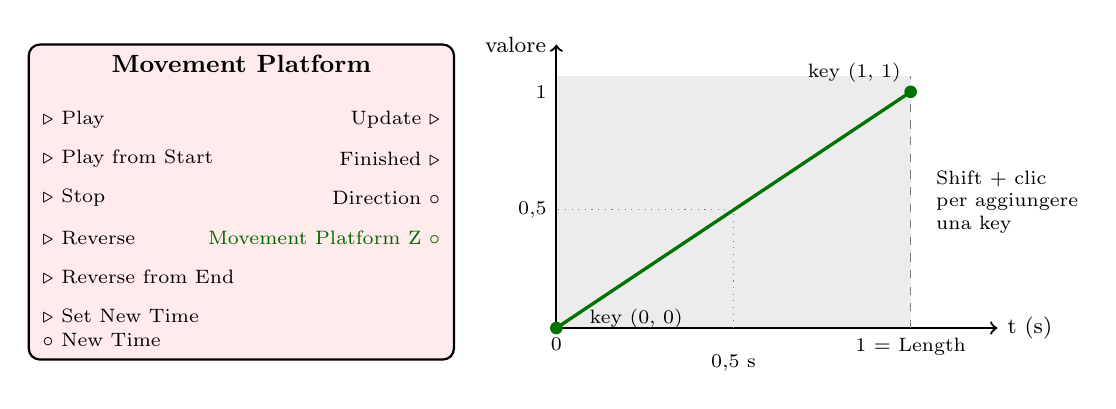
\begin{tikzpicture}[font=\footnotesize,
  ue6tl/.style={draw, thick, rounded corners=4pt, fill=red!8, minimum width=5.4cm,
                minimum height=4.0cm},
  ue6pin/.style={font=\scriptsize}]
  % nodo
  \node[ue6tl] (tl) at (0,0) {};
  \node[font=\small\bfseries] at (0,1.75) {Movement Platform};
  \foreach \t [count=\k] in {Play, Play from Start, Stop, Reverse, Reverse from End,
                             Set New Time} {
    \node[ue6pin, anchor=west] at (-2.65,1.55-0.5*\k) {$\triangleright$ \t};
  }
  \node[ue6pin, anchor=west] at (-2.65,-1.75) {$\circ$ New Time};
  \node[ue6pin, anchor=east] at (2.65,1.05) {Update $\triangleright$};
  \node[ue6pin, anchor=east] at (2.65,0.55) {Finished $\triangleright$};
  \node[ue6pin, anchor=east] at (2.65,0.05) {Direction $\circ$};
  \node[ue6pin, anchor=east, text=green!40!black] at (2.65,-0.45) {Movement Platform Z
    $\circ$};
  % curva
  \begin{scope}[xshift=4.0cm, yshift=-1.6cm]
    \fill[gray!15] (0,0) rectangle (4.5,3.2);
    \draw[->, thick] (0,0) -- (5.6,0) node[right]{t (s)};
    \draw[->, thick] (0,0) -- (0,3.6) node[left]{valore};
    \draw[gray, dashed] (4.5,0) -- (4.5,3.2);
    \node[font=\scriptsize, below] at (4.5,0) {1 = Length};
    \node[font=\scriptsize, below] at (0,0) {0};
    \node[font=\scriptsize, left] at (0,3.0) {1};
    \node[font=\scriptsize, left] at (0,1.5) {0,5};
    \draw[very thick, green!45!black] (0,0) -- (4.5,3.0);
    \fill[green!45!black] (0,0) circle (0.08);
    \fill[green!45!black] (4.5,3.0) circle (0.08);
    \node[font=\scriptsize, right] at (0.3,0.12) {key (0, 0)};
    \node[font=\scriptsize, above left] at (4.5,3.0) {key (1, 1)};
    \draw[gray, dotted] (2.25,0) -- (2.25,1.5) -- (0,1.5);
    \node[font=\scriptsize, align=center] at (2.25,-0.45) {0,5 s};
    \node[font=\scriptsize, align=left, anchor=west] at (4.7,1.6) {Shift + clic\\per
      aggiungere\\una key};
  \end{scope}
\end{tikzpicture}
\caption{Il nodo Timeline della piattaforma e la sua float track. A sinistra i sei
ingressi di esecuzione e le uscite: Update, Finished, Direction e il pin della traccia.
A destra la curva: Length 1 secondo (la zona grigia), due key in (0, 0) e (1, 1); a metà
del tempo il valore è a metà. Schema ricostruito.}
\label{ue6:fig:timeline}
\end{figure}

\begin{table}[htbp]
\centering
\small
\begin{tabular}{@{}p{3.4cm}p{10.6cm}@{}}
\toprule
\textbf{Pin} & \textbf{Che cosa fa} \\
\midrule
Play & riprende dal tempo attuale, in avanti \\
Play from Start & torna a 0 e va in avanti \\
Stop & ferma la timeline dove si trova \\
Reverse & riprende dal tempo attuale, all'indietro \\
Reverse from End & salta alla fine e va all'indietro \\
Set New Time & porta la timeline al tempo New Time \\
\midrule
Update & scatta a ogni aggiornamento mentre la timeline scorre \\
Finished & scatta quando la timeline arriva a un estremo (la fine in avanti, l'inizio
all'indietro) \\
Direction & la direzione attuale: Forward o Backward (un'enumerazione,
\emph{ETimelineDirection}) \\
una uscita per traccia & il valore della traccia al tempo attuale (float, vettore,
colore); le Event track hanno invece un'uscita di esecuzione \\
\bottomrule
\end{tabular}
\caption{I pin del nodo Timeline.}
\label{ue6:tab:timeline}
\end{table}

\paragraph{Approfondimento: le timeline secondo Romero e Sewell.} Nel capitolo 6
(\emph{Enhancing Player Abilities}) i due autori usano una timeline per lo
\emph{zoom} del mirino: una float track \emph{Field of View} da 90 a 45 in 0,3 secondi,
collegata dall'Update al nodo \emph{Set Field of View}, con il tasto premuto su Play e il
tasto rilasciato su \textbf{Reverse}, esattamente lo schema che la lezione userà per la
piattaforma che sale e scende. Il libro aggiunge due osservazioni. La prima: le timeline
sono perfette ``per semplici cambi di valore, come la rotazione di una porta''; per
animazioni complesse, di personaggi o cinematiche, Unreal ha il \textbf{Sequencer}. La
seconda (nella tabella che confronta macro, funzioni ed eventi): i nodi Timeline si
possono usare solo nell'\textbf{Event Graph} di un actor, non dentro le funzioni né
dentro le macro, perché, come i Delay, sono azioni che durano nel tempo. Nelle opzioni
in cima all'editor ci sono poi \textbf{Auto Play} (parte da sola al Begin Play),
\textbf{Loop} (ricomincia all'infinito, utile per un'altalena) e \textbf{Use Last
Keyframe} (fa finire la timeline sull'ultima key invece che alla Length). Le key, con il
tasto destro, possono avere interpolazione lineare, costante o \emph{auto} (curva
morbida, con le tangenti): una curva a ``S'' fa partire e arrivare la piattaforma
dolcemente, invece che di colpo.

% ---------------------------------------------------------------------
\section{L'interpolazione lineare e l'alfa}
\label{ue6:sec:lerp}

``Adesso ci servirebbe fare quello che viene chiamato, in informatica e anche su Unreal,
\textbf{interpolazione}.'' C'è una slide: l'\textbf{interpolazione lineare} ``ci dice:
passo da questo punto a questo punto, passandomi per tutti gli intermedi'', con un
\textbf{alfa}.

\paragraph{L'esempio delle animazioni.} ``L'interpolazione è un concetto che possiamo
trovare in tante cose diverse, tra cui le animazioni.'' Per muovere gli arti di un
personaggio si usano le \textbf{ossa}, interne alla \emph{mesh}. Il docente muove il
braccio davanti alla webcam: ``io non è che vedo subito così, pa!, di scatto: passo
proprio da questo a questo''. ``L'interpolazione è il passaggio per tutti i punti
intermedi che mi fa arrivare alla posizione finale.''

\paragraph{L'alfa.} ``Seguitemi bene attentamente, ragazzi.'' Su una linea che va da 0 a
100, l'alfa è ``un \textbf{puntatore} del punto in cui ci troviamo'', espresso da 0 a 1.
Se siamo a 0, l'alfa è 0; se siamo a 100, l'alfa è 1; ``se l'alfa sta a 0,5, ci
troveremo alla sua metà''. Domanda: se siamo a 20? Uno studente: ``0,2''. ``Ottimo. Siamo
a 0,2: l'alfa sarà a 0,2.'' ``Ci sono varie tipologie di interpolazione, ma
l'interpolazione funziona in questo modo'' (figura~\ref{ue6:fig:lerp}).

\begin{figure}[htbp]
\centering
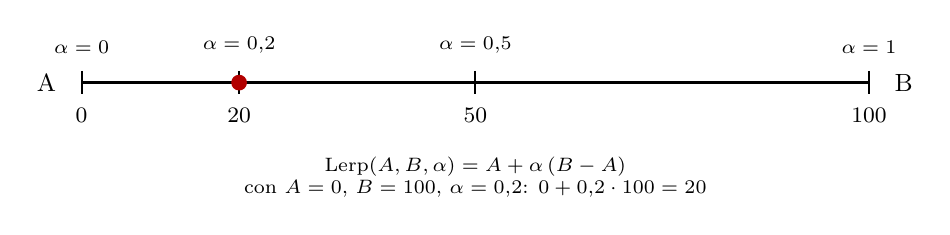
\begin{tikzpicture}[font=\footnotesize]
  \draw[very thick] (0,0) -- (10,0);
  \foreach \x/\l in {0/0, 2/20, 5/50, 10/100} {
    \draw[thick] (\x,0.15) -- (\x,-0.15);
    \node[below] at (\x,-0.2) {\l};
  }
  \node[above, font=\scriptsize] at (0,0.25) {$\alpha = 0$};
  \node[above, font=\scriptsize] at (2,0.25) {$\alpha = 0{,}2$};
  \node[above, font=\scriptsize] at (5,0.25) {$\alpha = 0{,}5$};
  \node[above, font=\scriptsize] at (10,0.25) {$\alpha = 1$};
  \node[left, font=\small] at (-0.2,0) {A};
  \node[right, font=\small] at (10.2,0) {B};
  \fill[red!70!black] (2,0) circle (0.1);
  \node[align=center, font=\scriptsize] at (5,-1.2) {$\mathrm{Lerp}(A, B, \alpha) = A +
    \alpha\,(B - A)$\\con $A = 0$, $B = 100$, $\alpha = 0{,}2$: $0 + 0{,}2 \cdot 100 =
    20$};
\end{tikzpicture}
\caption{L'alfa dell'interpolazione lineare: un numero da 0 a 1 che dice in che punto
del segmento da A a B ci troviamo. L'esempio della lezione: a 20 su 100 l'alfa vale
0,2. La formula, sotto, non è stata scritta a lezione ma è quella che il nodo Lerp
calcola. Schema ricostruito.}
\label{ue6:fig:lerp}
\end{figure}

\paragraph{Approfondimento: Lerp, alfa e timeline.} Il nodo \textbf{Lerp} (per i float)
calcola $A + \alpha(B - A)$: con $\alpha = 0$ restituisce A, con $\alpha = 1$
restituisce B, e in mezzo i valori intermedi in proporzione. Esiste per i vettori
(\textbf{Lerp (Vector)}, che interpola X, Y e Z con lo stesso alfa), per le rotazioni
(\textbf{Lerp (Rotator)}, con l'opzione \emph{Shortest Path}), per i colori e per i
\emph{transform}. L'alfa può anche uscire da $[0, 1]$: con 1,2 il risultato va oltre B
(estrapolazione). Il binomio timeline--Lerp è classico perché divide i compiti: la
\textbf{timeline} decide \emph{come} si scorre nel tempo (quanto dura, con che curva,
avanti o indietro), il \textbf{Lerp} decide \emph{dove} si va (da A a B). Cambiare la
durata o la forma del movimento non tocca A e B, e viceversa. Da non confondere con i nodi
\emph{FInterp To} e \emph{RInterp To} (quest'ultimo usato per la torretta): quelli
avvicinano ogni frame un valore al bersaglio di una frazione, con una velocità e il
Delta Time, senza un alfa né una durata fissa.

% ---------------------------------------------------------------------
\section{Il primo metodo: un Lerp sulla Z}
\label{ue6:sec:metodo1}

``Abbiamo quindi da tirare fuori il nostro bellissimo \textbf{Lerp}.'' Domanda di
partenza, guardando la piattaforma: ``quale asse dovremmo influenzare, che si muova nel
tempo?'' ``La Z.'' ``Ottimo, bravo, Federico.''

\paragraph{La costruzione.} Il docente procede per tentativi, e a un certo punto uno
studente chiede: ``potresti spiegare un po' tutti i passaggi? Perché a un certo punto mi
sono perso''. La versione rispiegata, che è quella da seguire, è questa
(figura~\ref{ue6:fig:metodo1}).
\begin{enumerate}
  \item Si prende il componente \textbf{Platform} e si tira fuori \textbf{Get Relative
        Location}. All'inizio il docente aveva usato Get Actor Location, poi la World
        Location (``scusate, ragazzi, questa è world''), e infine la \emph{relative},
        cioè la posizione rispetto all'actor. Si splitta il vettore.
  \item La \textbf{Z} relativa va, da sola, nel pin \textbf{A} del Lerp: il punto di
        partenza.
  \item La stessa Z più una variabile float nuova, \textbf{MaxHeight}, va nel pin
        \textbf{B}: il punto d'arrivo. Il valore scelto è \textbf{70} (``ci piace 70'';
        ``sono 70 unità sulla Z'').
  \item L'\textbf{Alpha} del Lerp è il pin \textbf{Movement Platform Z} della timeline.
  \item Un \textbf{Make Vector}: X e Y dalla location relativa, invariate; Z dal Lerp.
  \item \textbf{Set Relative Location} sul componente Platform, con il Make Vector nel
        pin \emph{New Location}, eseguito dall'\textbf{Update} della timeline.
\end{enumerate}
La timeline parte dal Begin Overlap della box, attraverso il Branch sul player, con
\textbf{Play}.

\begin{figure}[htbp]
\centering
\begin{tikzpicture}[font=\footnotesize,
  ue6node/.style={draw, thick, rounded corners=4pt, align=center, fill=gray!8,
                  minimum height=0.8cm, text width=2.1cm},
  ue6event/.style={ue6node, fill=red!12},
  ue6exec/.style={-{Stealth[length=2.5mm]}, very thick, black!80},
  ue6data/.style={-{Stealth[length=2mm]}, thick, green!45!black},
  ue6vec/.style={-{Stealth[length=2mm]}, thick, yellow!50!black}]
  \node[ue6event, text width=2.5cm] (ov) at (0,0) {\textbf{On Component Begin
    Overlap} (Box)};
  \node[ue6node, text width=2.4cm] (eq) at (0,-1.8) {Other Actor \textbf{==}\\\textbf{Get
    Player Pawn}};
  \node[ue6node, text width=1.3cm] (br) at (3.0,0) {\textbf{Branch}};
  \node[ue6node, text width=2.3cm] (tl) at (5.8,0) {\textbf{Timeline}\\Movement
    Platform};
  \node[ue6node, text width=2.4cm] (set) at (11.0,0) {\textbf{Set Relative
    Location}\\(Platform)};
  \node[ue6node, text width=2.5cm] (grl) at (3.0,-3.6) {Platform $\rightarrow$
    \textbf{Get Relative Location} (split)};
  \node[ue6node, text width=1.8cm] (mh) at (5.8,-3.6) {Z +\\\textbf{MaxHeight} (70)};
  \node[ue6node, text width=1.4cm] (lerp) at (8.2,-2.0) {\textbf{Lerp}\\A, B, Alpha};
  \node[ue6node, text width=1.7cm] (mv) at (11.0,-2.0) {\textbf{Make Vector}};
  \draw[ue6exec] (ov) -- (br);
  \draw[ue6exec] (br) -- node[above, font=\scriptsize]{True} node[below,
    font=\scriptsize]{Play} (tl);
  \draw[ue6exec] (tl) -- node[above, font=\scriptsize]{Update} (set);
  \draw[-{Stealth[length=2mm]}, thick, red!60!black] (eq.north) -- node[right,
    font=\scriptsize]{bool} (br.south west);
  \draw[ue6data] (tl.south) -- node[left, font=\scriptsize, pos=0.3]{Z track} (lerp.west);
  \draw[ue6data] (grl.north) |- node[pos=0.25, left, font=\scriptsize]{Z $\rightarrow$ A}
    ([yshift=-0.2cm]lerp.west);
  \draw[ue6data] (grl) -- (mh);
  \draw[ue6data] (mh.east) -| node[pos=0.7, right, font=\scriptsize]{B} (lerp.south);
  \draw[ue6data] (lerp) -- node[above, font=\scriptsize]{Z} (mv);
  \draw[ue6data] (grl.south) -- ++(0,-0.35) -| node[pos=0.25, below,
    font=\scriptsize]{X, Y} (mv.south);
  \draw[ue6vec] (mv) -- node[right, font=\scriptsize]{New Location} (set);
\end{tikzpicture}
\caption{Il primo metodo. Il Begin Overlap della box, se l'actor è il player, fa
partire la timeline; a ogni Update un Lerp tra la Z relativa attuale (A) e la stessa Z
più MaxHeight (B), con la traccia della timeline come alfa, diventa la nuova Z della
Platform. Funziona, ma ha un difetto: A e B vengono riletti a ogni Update dalla posizione
già spostata (vedi l'approfondimento). Schema ricostruito.}
\label{ue6:fig:metodo1}
\end{figure}

\paragraph{``Va altissimo''.} In Play la piattaforma sale, ma molto più di 70 unità: a uno
studente, con 70, ``arriva in cielo''; con 30 arriva ``poco più alto del muretto'' della
scena. ``Non so perché, però sia così diverso.'' Il docente promette un metodo ``un po'
più carino e più malleabile''; la spiegazione arriva, in parte, dopo la pausa: ``stiamo
sommando'' (sezione~\ref{ue6:sec:playrate}).

\paragraph{Approfondimento: perché il primo metodo ``somma''.} A ogni Update il grafo
legge la Z \emph{attuale} della Platform, che è già stata spostata dall'Update
precedente, e la usa come A; B è quella Z più 70. Il risultato è quindi
$Z_{\text{nuova}} = Z_{\text{attuale}} + \alpha \cdot 70$: non un punto tra due estremi
fissi, ma un \emph{incremento} che si accumula. Se la timeline si aggiorna $N$ volte in
un secondo, la piattaforma sale di circa $70 \cdot \sum \alpha_k \approx 70 \cdot N/2$
unità: con 60 aggiornamenti al secondo, più di duemila, non settanta. Da qui tre
conseguenze, tutte osservate a lezione. La salita dipende dal \emph{frame rate} (``è la
mia impressione che vada più in alto'': su un computer più veloce, più somme). Rallentare
la timeline con il play rate fa \emph{più} somme, e la piattaforma sale ancora di più;
accelerarla ne fa meno. E con il Reverse il calcolo non torna simmetrico: lo studente
che si vedeva la piattaforma ``sempre leggermente più in basso fino a scomparire sotto il
terreno'' stava osservando proprio l'errore che si accumula a ogni salita e discesa. La
cura è leggere A e B \emph{una volta sola}, prima che la timeline parta, e tenerli fissi:
è il secondo metodo.

% ---------------------------------------------------------------------
\section{La pausa e il Nintendo Direct}
\label{ue6:sec:pausa}

``Sono le 17:37. Facciamo la pausa classica di 20 minuti''; si torna ``alle 18''. Durante
la pausa il docente aiuta uno studente con la foto del codice mandata su Discord (il
problema è l'altezza della piattaforma con il primo metodo: ``70 è giusto'', il resto
``credo sia tutto giusto''), e poco prima della ripresa arrivano le notizie dal
\emph{Nintendo Direct}, riferite da uno studente ``referente''. Nella trascrizione,
molto storpiata, si riconoscono un \emph{remake} di \emph{Ocarina of Time} (``l'Opera of
Time Remake''), un nuovo \emph{Xenoblade}, un \emph{Final Fantasy} in 2D-HD ``stile
\emph{Octopath Traveler}'' e del materiale nuovo su \emph{Deltarune}; il tutto è riportato
come lo si legge nella trascrizione, senza verifiche. La chiacchierata scivola su
\emph{Kingdom Hearts} e sulla trilogia \emph{remake} di \emph{Final Fantasy VII} (``uscirà
prima l'intera trilogia remake''), e su Tetsuya Nomura (``le nomurate''). ``Comunque,
sempre belli questi siparietti'', dice il docente; chi segue in differita può
partecipare alla conversazione su Discord, ``pacificamente''.

% ---------------------------------------------------------------------
\section{La velocità della timeline: Set Play Rate e Duration}
\label{ue6:sec:playrate}

``Allora riprendiamo la nostra bellissima \emph{elevator}, o piattaforma, quello che
vogliamo.'' Una cosa che si può controllare è il \textbf{play rate}: ``la velocità in cui
essa, sempre ripetendo un secondo, viene detta: vai a due volte la tua velocità, a metà
della tua velocità''.

\paragraph{La timeline è un componente.} ``Se avete notato'', nel pannello
\textbf{Components} del Blueprint, accanto a Box, Platform e DefaultSceneRoot, c'è anche
\textbf{Movement Platform}: ``lo stesso nome della timeline''. Ogni timeline aggiunta
crea un componente con il suo nome, e da quel componente si possono chiamare le sue
funzioni. Trascinandolo nel grafo (``Ctrl per il Get''), se ne tira fuori \textbf{Set
Play Rate}, con il \emph{Target} sulla timeline.

\paragraph{Play rate e lunghezza.} Sul \textbf{Begin Play}, Set Play Rate a 0,5: ``la
sua velocità sarà la metà''; a 2, ``il doppio''; a 1, ``andrà come prima''. Il docente
insiste: ``il play rate \textbf{non è la lunghezza}, non è la Length, è diversa''. La
Length dice quanto è lunga la curva; il play rate dice quanto velocemente la si
percorre.

\paragraph{Il primo metodo non regge.} Con il play rate cambiato, la piattaforma del primo
metodo si comporta in modo strano, e il docente ne dà la spiegazione: ``stiamo
aumentando di 30 a ogni frame del nostro secondo''; ``se riduciamo il play rate, lui
sarà più veloce, ma di conseguenza farà meno somme''. Detto meglio: con un play rate più
alto la timeline finisce prima, fa meno Update, e quindi meno somme; con uno più basso ne
fa di più. ``Vedete che non si ferma a quell'unità, perché in questo caso stiamo sommando
solamente: se finisce prima, vuol dire che finirà prima.''

\paragraph{La variabile Duration.} Ragionare in velocità relative è scomodo; è più
naturale dire ``voglio che duri 2 secondi''. Una variabile float \textbf{Duration} e un
piccolo calcolo:
\[
  \text{Play Rate} = \frac{1}{\text{Duration}} \times \text{Timeline Length},
\]
con \textbf{Divide} (``lo slash'') e \textbf{Get Timeline Length} (dal componente della
timeline) moltiplicati con \textbf{Multiply}, e il risultato nel Set Play Rate del Begin
Play. Con Duration 1 e una Length di 1 il play rate è 1, ``velocità normale''. Con
Duration 2 il docente prima dice ``il doppio'', poi si corregge: ``no, scusa, sarà più
lunga, perdonate''; con 0,5 sarà più veloce. È ``una variabile d'appoggio'' che traduce
una durata in secondi nel play rate giusto. Per il resto della lezione la Duration resta
a 1, ``così almeno siamo tranquilli''.

\paragraph{Approfondimento: perché la formula funziona.} Una timeline di lunghezza $L$
percorsa con play rate $r$ dura $L / r$ secondi. Volendo che duri $D$ secondi, basta
porre $L / r = D$, cioè $r = L / D$: è la formula del docente, scritta come $1/D \times
L$. Moltiplicare per la Length rende il calcolo indipendente dalla curva: se un giorno la
timeline diventa lunga 3 secondi, la Duration continua a dire la durata vera. Due
cautele. Una Duration a 0 produce una divisione per zero, e la timeline non si muove più
(il primo sospetto, a lezione, quando la piattaforma di uno studente ``ha smesso di
muoversi''). E il Set Play Rate va chiamato sulla timeline \emph{giusta}: è l'errore
della sezione~\ref{ue6:sec:timelinesbagliata}.

% ---------------------------------------------------------------------
\section{Il secondo metodo: il Billboard e le posizioni salvate}
\label{ue6:sec:metodo2}

Per avere ``due punti specifici da raggiungere, in modo non dipendente da dei valori'',
il docente rifà il grafo. Il vecchio si può tenere, staccato, e copiare (``Ctrl+C,
Ctrl+V'') i pezzi che servono; il Set Relative Location della Platform resta: ``non lo
cancellate, perché è giusto che sia così''.

\paragraph{Il Billboard.} Si aggiunge (\emph{Add}) un componente \textbf{Billboard}:
``un oggetto di questo tipo: è questo \textbf{dinosauro}''. ``Fondamentalmente è un punto
nello spazio'', come lo \emph{Scene Component} già usato per la torretta; ``la
differenza è che ha un'immagine'', visibile solo nell'editor. Il piano: ``prendere la sua
posizione nello spazio, e dire: \emph{lerpami} da questa posizione della piattaforma
iniziale a questa posizione del billboard''. Il Billboard si mette a \textbf{500} sulla
Z (``o di più? 700? Mettete 500, la metà è giusta'').

\paragraph{Lerp (Vector).} Al posto del Lerp sui float, un \textbf{Lerp (Vector)} (``un
v-lerp, un lerp tra vettori''): ``invece che tra due numeri, due float, tra due
vettori''. A è la \textbf{Get Relative Location} della Platform, B quella del Billboard,
l'Alpha la traccia della timeline; l'uscita va direttamente nel Set Relative Location
della Platform, senza Make Vector.

\paragraph{``C'è qualcosa di sbagliato?''} Così com'è, avverte il docente, il grafo ha
ancora il difetto del primo metodo: ``non salviamo mai la posizione delle due''. Se il
Billboard fosse \textbf{attaccato} alla Platform, ``si muoverà insieme ad essa'', e
allora ``avremo un effetto infinito'': la piattaforma insegue un bersaglio che si
allontana, ``un continuo movimento sempre in alto, sempre in alto, pom pom pom''. Il
docente lo mostra riattaccando il Billboard: ``e si ricomincia''. La cura:
\begin{enumerate}
  \item i due Get Relative Location si spostano sul \textbf{Begin Play};
  \item sul pin di uscita di ciascuno, \textbf{Promote to Variable}: la Platform diventa
        \textbf{StartLocation}, il Billboard \textbf{FinishLocation};
  \item nel Lerp (Vector) entrano i \emph{Get} delle due variabili: StartLocation in A,
        FinishLocation in B.
\end{enumerate}
``Così facendo abbiamo delle variabili che sono sempre fisse'': ``sarà sempre la stessa
posizione'' (figura~\ref{ue6:fig:metodo2}).

\paragraph{Il bello del Billboard.} ``La cosa bella, poi, che possiamo vedere con questo
metodo'': il dinosauro si può spostare nello spazio, nei dettagli della piattaforma, e la
piattaforma raggiungerà quel punto. ``Dovete fare un livello? L'avete alzato a 8 metri?
Prendete il billboard, lo mettete a 800'': ``devo arrivare qua sopra, quindi arriverò
qua. Ecco fatto, sono arrivato preciso''. (``Salto, l'ho mancato malissimo.'') E non solo
in verticale: spostando il Billboard anche sulla X o sulla Y, ``andrà in diagonale'';
``potremmo pure fare piattaforme in orizzontale, in diagonale, come vi pare''. ``Invece
di fare matematica'', si prendono direttamente i due vettori.

\paragraph{Il ritorno: Reverse.} Scendendo dalla piattaforma, questa ``rimane là''.
``Vi potrei dire: facciamo una nuova timeline e la facciamo al contrario. Non serve.
Perché abbiamo \textbf{Reverse}.'' L'\textbf{On Component End Overlap} della box,
collegato al pin Reverse della timeline: ``esco fuori e lei se ne torna al suo posto'',
perché ``invece di fare da A a B, fa da B ad A. Questo è insito nella timeline''.

\begin{figure}[htbp]
\centering
\begin{tikzpicture}[font=\footnotesize,
  ue6node/.style={draw, thick, rounded corners=4pt, align=center, fill=gray!8,
                  minimum height=0.8cm, text width=2.1cm},
  ue6event/.style={ue6node, fill=red!12},
  ue6var/.style={ue6node, fill=blue!10, rounded corners=8pt},
  ue6exec/.style={-{Stealth[length=2.5mm]}, very thick, black!80},
  ue6data/.style={-{Stealth[length=2mm]}, thick, green!45!black},
  ue6vec/.style={-{Stealth[length=2mm]}, thick, yellow!50!black}]
  % Begin Play
  \node[ue6event, text width=2.4cm] (bp) at (0,0) {\textbf{Event Begin Play}};
  \node[ue6node, text width=2.3cm] (s1) at (3.3,0) {\textbf{Set}\\StartLocation};
  \node[ue6node, text width=2.3cm] (s2) at (6.4,0) {\textbf{Set}\\FinishLocation};
  \node[ue6node, text width=2.2cm] (pr) at (9.6,0) {\textbf{Set Play Rate}\\($1/D \times
    L$)};
  \node[ue6node, text width=2.5cm] (g1) at (3.3,-1.6) {Platform $\rightarrow$ Get
    Relative Location};
  \node[ue6node, text width=2.5cm] (g2) at (6.4,-1.6) {Billboard $\rightarrow$ Get
    Relative Location};
  \draw[ue6exec] (bp) -- (s1);
  \draw[ue6exec] (s1) -- (s2);
  \draw[ue6exec] (s2) -- (pr);
  \draw[ue6vec] (g1) -- (s1);
  \draw[ue6vec] (g2) -- (s2);
  % overlap e timeline
  \begin{scope}[yshift=-3.6cm]
    \node[ue6event, text width=2.6cm] (bo) at (-0.2,0) {\textbf{Begin Overlap}
      (Box)\\+ Branch sul player};
    \node[ue6event, text width=2.6cm] (eo) at (-0.2,-1.5) {\textbf{End Overlap} (Box)};
    \node[ue6node, text width=2.2cm, minimum height=2.2cm] (tl) at (3.6,-0.75)
      {\textbf{Timeline}\\Movement\\Platform};
    \node[ue6node, text width=1.9cm] (lv) at (7.0,-2.5) {\textbf{Lerp (Vector)}\\A, B,
      Alpha};
    \node[ue6var, text width=1.9cm] (v1) at (7.0,-4.0) {StartLocation};
    \node[ue6var, text width=2.1cm] (v2) at (9.8,-4.0) {FinishLocation};
    \node[ue6node, text width=2.4cm] (set) at (10.4,-0.4) {\textbf{Set Relative
      Location}\\(Platform)};
    \draw[ue6exec] (bo.east) -- node[above, font=\scriptsize]{Play} ([yshift=0.75cm]tl.west);
    \draw[ue6exec] (eo.east) -- node[below, font=\scriptsize]{Reverse}
      ([yshift=-0.75cm]tl.west);
    \draw[ue6exec] ([yshift=0.35cm]tl.east) -- node[above, font=\scriptsize]{Update}
      (set.west);
    \draw[ue6data] ([yshift=-0.6cm]tl.east) -| node[pos=0.25, above,
      font=\scriptsize]{Alpha} (lv.north);
    \draw[ue6vec] (v1) -- node[left, font=\scriptsize]{A} (lv);
    \draw[ue6vec] (v2.north) |- node[pos=0.25, right, font=\scriptsize]{B} (lv.east);
    \draw[ue6vec] (lv.east) -- ++(0.9,0) |- node[pos=0.2, right,
      font=\scriptsize]{New Location} (set.south west);
  \end{scope}
\end{tikzpicture}
\caption{Il secondo metodo. Sopra: al Begin Play le posizioni relative della Platform e
del Billboard vengono salvate una volta per tutte in StartLocation e FinishLocation (con
Promote to Variable), e si imposta il play rate dalla Duration. Sotto: il Begin Overlap
fa Play, l'End Overlap fa Reverse; a ogni Update un Lerp (Vector) tra i due punti fissi,
con la traccia come alfa, diventa la nuova posizione della Platform. Schema
ricostruito.}
\label{ue6:fig:metodo2}
\end{figure}

\paragraph{I problemi.} ``Problemi su questo? Siete a posto?'' Tre casi.
\begin{itemize}
  \item \textbf{``A me non si muove.''} Il docente ripassa la lista: le due Get Relative
        Location, le due variabili, la timeline in Play, l'Update, il Lerp tra i
        vettori, l'Alpha collegato. Lo studente non aveva capito come creare le
        variabili: tasto destro sul pin, \textbf{Promote to Variable}, e il nome. Poi
        StartLocation in A, FinishLocation in B, e l'Alpha alla traccia della timeline.
  \item \textbf{L'evento diventato Custom Event.} Uno studente scopre da solo il suo
        errore: copiando e incollando il blocco, l'evento di overlap ``mi ha preso come
        Custom Event generico, e quindi non si muoveva''. Un evento di componente
        incollato in un Blueprint perde il legame con il componente e diventa un evento
        qualunque, che nessuno chiama. ``Errore di distrazione.''
  \item \textbf{Ero rimasto indietro.} Uno studente, che aveva ricevuto una telefonata,
        riceve il riassunto: Billboard, Get Relative Location della Platform in
        StartLocation e del Billboard in FinishLocation, il Lerp (Vector) con l'alfa, il
        Set Relative Location, e il Reverse sull'End Overlap.
\end{itemize}

\paragraph{Approfondimento: Billboard figlio di chi?} Il docente fa vedere che, con il
Billboard attaccato alla Platform, la piattaforma ``sale all'infinito'', e che salvando le
posizioni al Begin Play il problema scompare. Ma c'è un dettaglio che la lezione non
esplicita: se il Billboard resta figlio della Platform, la sua \emph{relative location}
è relativa alla Platform, non all'actor; salvarla al Begin Play dà $(0, 0, 500)$ rispetto
alla piattaforma, mentre il Set Relative Location della Platform lavora rispetto alla
radice dell'actor. I due numeri coincidono solo se la Platform sta nell'origine
dell'actor (come nel Blueprint della lezione). La configurazione più robusta è mettere il
Billboard come figlio della \textbf{DefaultSceneRoot}, accanto alla Platform, così che
le due posizioni relative siano nello stesso spazio e il bersaglio non si muova mai con
la piattaforma. Un'altra soluzione, equivalente, è salvare e impostare le posizioni nel
mondo (Get e Set World Location). Infine: il ``dinosauro'' è visibile solo nell'editor;
nel gioco il Billboard non si vede, come tutti i componenti di servizio.

% ---------------------------------------------------------------------
\section{La timeline sbagliata}
\label{ue6:sec:timelinesbagliata}

Il docente vuole far vedere che la Duration funziona anche con il secondo metodo: ``la
cambio in 2''; poi, ``mettiamo dei valori che posso riconoscere, tipo 10''. Ma la
velocità non cambia. ``Non mi setta il play rate, forse.'' Anche a uno studente,
``l'unica cosa è la duration: non va effettivamente a modificare la velocità''. Il
docente prova un Print, un play rate a 0,1, a mille: ``sempre lo stesso''.

\paragraph{La soluzione, da uno studente.} ``Domanda un po' stupida: non è che forse
l'attore deve essere Platform e non Movement Platform?'' Non è quello, ma è la pista
giusta: ``errore mio''. Il secondo metodo usa una timeline \emph{nuova}, che si chiama
semplicemente \textbf{Timeline}; il Set Play Rate del Begin Play aveva come Target ancora
\textbf{Movement Platform}, ``quella dell'esempio di prima''. ``Stavamo referenziando la
timeline dell'altro esempio, e non la playavamo mai.''

\paragraph{La lezione dell'errore.} ``Da questo errore possiamo imparare qualche cosa'':
``le timeline hanno un \textbf{nome}''. Ogni timeline è un componente distinto, e le sue
funzioni (Set Play Rate, Get Timeline Length, Play, Reverse\ldots) agiscono solo su di
lei. Con il Target giusto e una Duration di 3, la piattaforma ``adesso è più lenta,
perché dura di più''. Morale: dare alle timeline nomi chiari, e cancellare quelle che non
servono più.

% ---------------------------------------------------------------------
\section{L'audio: la Sound Cue}
\label{ue6:sec:cue}

``Se non ci sono più problemi, passiamo al nostro bellissimo \emph{sound}.''

\paragraph{Importare il file.} Un consiglio d'ordine: una \textbf{cartella audio} nel
Content Browser (tasto destro, \emph{New Folder}). Per importare il file scaricato da
Discord basta \textbf{trascinarlo} nel Content Browser: appare un asset ``con la linea'',
una \textbf{Sound Wave}, senza altre domande.

\paragraph{Creare la Cue.} Sulla Sound Wave, tasto destro, \textbf{Create Cue} (``è il
secondo''). La \textbf{Sound Cue} (``la queue'', ``la Q'', nella trascrizione) è, dice il
docente, ``un \emph{sound} programmabile, tra virgolette''. Doppio clic: si apre un grafo
``come abbiamo visto anche su Unreal molto spesso'', con un nodo \textbf{Wave Player}
(il nostro suono) collegato all'\textbf{Output}. A sinistra, i dettagli della Cue:
\textbf{Volume Multiplier}, \textbf{Pitch Multiplier}, \emph{Sound Class} (``class
override''), \emph{Attenuation} e così via, ``tutti i vari dati che possiamo
modificare''.

\paragraph{Il pitch.} Con il Pitch Multiplier a 2 il suono è più alto; a 0,5 ``è pitchato
verso il basso'': ``molto più basso livello di tono, e anche più lento''. ``Perché il
pitch influenza sia la velocità sia la tonalità.'' Si torna a 1.

\paragraph{Il loop.} Con Play il suono parte ``solo una volta''; ``noi vogliamo che vada
in loop'' finché la piattaforma si muove, ``tipo: pipi, pipi, pipi''. Sul nodo
\textbf{Wave Player} si spunta \textbf{Looping}. (``Ovviamente rompe'': con la barra
spaziatrice si avvia e si interrompe l'anteprima.)

\paragraph{Il Modulator.} ``Vogliamo che magari il pitch o il volume siano un valore
\textbf{randomico}, tra un valore e un altro, in modo che non sia sempre lo stesso
suono.'' Si inserisce un nodo \textbf{Modulator} tra il Wave Player e l'Output: ha
\textbf{Pitch Min}, \textbf{Pitch Max}, \textbf{Volume Min} e \textbf{Volume Max}. I
valori della lezione: pitch tra \textbf{1,7} e \textbf{2}, volume tra \textbf{1} e
\textbf{1,2}. A ogni riproduzione il suono è ``leggermente più basso, leggermente più
alto''. Il perché, con il gioco della palla del docente: quando rimbalza fa un
\emph{boing}, ``e visto che avevo solo un suono'', che ripetuto ``sembra la stessa
cosa'', un pitch minimo e massimo hanno dato ``un risultato molto più gradevole''.

\paragraph{Il Random.} ``Esiste anche il \textbf{Random}'': se si hanno più suoni, il
nodo Random ne sceglie uno a caso a ogni riproduzione. Il docente lo prova mettendo nel
Random due rami, uno con il Modulator e uno senza, e ascoltando quale esce. L'uso tipico:
``un proiettile che prende un muro: invece di avere sempre lo stesso suono, mettete tutti
e tre i suoni nel Random''. Per la piattaforma non serve, e si torna al solo Modulator
(figura~\ref{ue6:fig:cue}).

\begin{figure}[htbp]
\centering
\begin{tikzpicture}[font=\footnotesize,
  ue6snode/.style={draw, thick, rounded corners=4pt, align=center, fill=violet!10,
                   minimum height=1.0cm, text width=2.5cm},
  ue6out/.style={draw, thick, rounded corners=4pt, align=center, fill=gray!20,
                 minimum height=1.0cm, text width=1.6cm},
  ue6aud/.style={-{Stealth[length=2.5mm]}, very thick, violet!60!black}]
  \node[ue6snode] (wp) at (0,0) {\textbf{Wave Player}\\SFX Moving Platform\\Looping
    \checkmark};
  \node[ue6snode] (mod) at (4.0,0) {\textbf{Modulator}\\Pitch 1,7--2\\Volume 1--1,2};
  \node[ue6out] (out) at (7.6,0) {\textbf{Output}};
  \draw[ue6aud] (wp) -- (mod);
  \draw[ue6aud] (mod) -- (out);
  \node[draw, dashed, rounded corners=4pt, align=left, text width=4.6cm, font=\scriptsize]
    at (11.4,0) {dettagli della Cue: Volume Multiplier, Pitch Multiplier (1), Sound
    Class, Attenuation\ldots};
  % variante random
  \begin{scope}[yshift=-2.4cm]
    \node[ue6snode, text width=2.0cm] (w1) at (0,0.6) {Wave Player 1};
    \node[ue6snode, text width=2.0cm] (w2) at (0,-0.6) {Wave Player 2};
    \node[ue6snode, text width=1.6cm] (rnd) at (4.0,0) {\textbf{Random}};
    \node[ue6out] (out2) at (7.6,0) {\textbf{Output}};
    \draw[ue6aud] (w1.east) -- (rnd.west);
    \draw[ue6aud] (w2.east) -- (rnd.west);
    \draw[ue6aud] (rnd) -- (out2);
    \node[align=left, font=\scriptsize, text width=4.6cm] at (11.4,0) {variante: più
      suoni, uno scelto a caso a ogni riproduzione (l'esempio del proiettile contro il
      muro)};
  \end{scope}
\end{tikzpicture}
\caption{La Sound Cue della piattaforma: il Wave Player in loop, un Modulator che varia
a caso pitch e volume a ogni riproduzione, l'Output. Sotto, la variante con il nodo
Random mostrata a lezione e poi scartata. Schema ricostruito.}
\label{ue6:fig:cue}
\end{figure}

\paragraph{Approfondimento: Sound Wave, Sound Cue, MetaSound.} La \textbf{Sound Wave} è
il file audio importato, con poche proprietà proprie (fra cui un suo \emph{Looping}). La
\textbf{Sound Cue} è un piccolo grafo che combina una o più Wave con nodi di
elaborazione: Modulator, Random, \emph{Mixer}, \emph{Concatenator}, \emph{Delay},
\emph{Attenuation}\ldots; nei Blueprint si può passare indifferentemente una Wave o una
Cue a qualunque nodo che vuole un \emph{Sound}. In Unreal Engine 5 esistono anche i
\textbf{MetaSound}, un sistema più recente e più potente, che genera e manipola l'audio
con un grafo simile a quello dei Blueprint; le Sound Cue restano supportate e sono il
punto di partenza più semplice. Il formato \textbf{WAV} raccomandato dal docente è quello
standard per l'import: non compresso, lo comprime poi l'engine secondo la piattaforma.
Sul pitch, l'osservazione del docente è esatta: in una Sound Cue il Pitch Multiplier
cambia la velocità di riproduzione, quindi alza o abbassa il tono e accorcia o allunga il
suono insieme, come un disco suonato a giri sbagliati.

% ---------------------------------------------------------------------
\section{Far suonare la piattaforma: Spawn Sound, Do Once e Stop}
\label{ue6:sec:suono}

``Abbiamo due modi per piazzare i suoni'': i nodi \textbf{Play Sound 2D} e \textbf{Play
Sound at Location}, e i nodi \textbf{Spawn Sound 2D} e \textbf{Spawn Sound at Location}.
``La differenza sostanziale è che uno \emph{playa} il suono solamente; l'altro lo
\emph{spawna}, e quindi crea una \textbf{referenza}'', come lo Spawn Actor from Class
``che quando spawna ha un Return Value''.

\paragraph{La prova con Play Sound 2D.} ``Proviamo a mettere Play Sound 2D'': la Cue
nel pin Sound, l'esecuzione dall'Update della timeline. Il docente sale sulla piattaforma: il suono parte,
``e non smette più''. Peggio: l'Update scatta a ogni aggiornamento, quindi i suoni si
sovrappongono (``come avete sentito, è stato uno stormo di uccelli incredibile''). Due
problemi, due soluzioni.
\begin{itemize}
  \item Il suono è in loop: per fermarlo bisogna sapere \emph{quale} suono fermare, e il
        Play Sound non lo dice. Serve lo \textbf{Spawn Sound at Location}, che
        restituisce la referenza.
  \item L'Update scatta molte volte: serve un \textbf{Do Once}, ``che lo fa una sola
        volta''.
\end{itemize}

\paragraph{Lo spawn.} \textbf{Do Once}, poi \textbf{Spawn Sound at Location}: Sound la
Cue, Location la \textbf{Get Actor Location} (``alla locazione dell'attore playerà questo
suono''; il docente pensa prima alla piattaforma, poi sceglie l'actor). Dal \textbf{Return
Value}, \textbf{Promote to Variable}: \textbf{SoundPlatform}. ``Adesso, di questo suono
che abbiamo creato, abbiamo la referenza: qualcosa che punta e ci dice: ehi, questo è il
suono che fa pipipipi.''

\paragraph{Lo stop.} ``Io voglio che si fermi quando la timeline finisce'', cioè quando
arriva in cima (a 1) o torna alla base (a 0). Sul \textbf{Finished} della timeline: Get
di SoundPlatform, \textbf{Stop}. ``Fino a che non è arrivato in cima, o fino a che non è
tornato alla base, il suono playerà, e si stopperà appena finisce la timeline.''

\paragraph{Il Reset del Do Once.} ``Un'ultima cosa molto importante.'' Il Do Once, una
volta passato, resta chiuso; ha però un ingresso \textbf{Reset}: ``se lo inserisco là
dentro, questo Do Once si resetta, si apre, e dà la possibilità di essere rieseguito''.
``Quando ho stoppato il suono una volta, lo devo riattivare per la volta dopo'': dopo lo
Stop, il Reset. ``E si ferma; scendo, ed eccolo. Benissimo.''

% ---------------------------------------------------------------------
\section{Il pitch che cambia con la direzione}
\label{ue6:sec:pitch}

``Potremmo anche, ipoteticamente\ldots'' L'idea: un suono \textbf{più alto quando la
piattaforma sale} e \textbf{più basso quando scende}. Il componente audio spawnato ha la
funzione \textbf{Set Pitch Multiplier}, da chiamare sulla referenza SoundPlatform.

\paragraph{Come sapere se sale o scende.} Il docente comincia a ragionare con un Branch
(``se sta andando da StartLocation a FinishLocation\ldots''), poi si ferma: ``possiamo
usare una cosa molto interessante''. Il pin \textbf{Direction} della timeline è
un'\textbf{enumerazione} (``che vedremo in seguito che cos'è, ma oggi ci serve
semplicemente vedere questa cosa''): ``una variabile che ha dentro di sé due elementi'',
\emph{Forward} e \emph{Backward}. Tirandone fuori uno \textbf{Switch on
ETimelineDirection} si ottengono due uscite di esecuzione: ``avanti vuol dire che sta
andando 0--1, e indietro è 1--0''.
\begin{itemize}
  \item \textbf{Forward}: Set Pitch Multiplier su SoundPlatform a \textbf{1}, il pitch
        normale;
  \item \textbf{Backward}: Set Pitch Multiplier a \textbf{0,4}, ``per far puh, puh, puh,
        un po' più bassino: una discesa'' (il docente prova anche 0,5 e 0,1, ``molto
        basso''; il valore finale è 0,4).
\end{itemize}
``Mettiamo tutto nel Do Once'' (figura~\ref{ue6:fig:suono}).

\paragraph{L'errore dell'ordine.} A una studentessa il grafo, ``sulla carta'', è giusto,
ma il compilatore segnala un errore: il Set Pitch Multiplier dice che il suono ``non è
mai stato creato''. Il motivo è l'ordine: lo Switch, con i due Set Pitch Multiplier,
veniva eseguito \emph{prima} che lo Spawn Sound avesse riempito la variabile, quindi su
una referenza vuota. ``Metti prima il Do Once'', e dopo lo spawn e il Set della
variabile, lo Switch con i due rami. ``Dovrebbe andare.'' E va (dopo aver condiviso anche
l'audio del computer su Zoom, per farlo sentire).

\begin{figure}[htbp]
\centering
\begin{tikzpicture}[font=\footnotesize,
  ue6node/.style={draw, thick, rounded corners=4pt, align=center, fill=gray!8,
                  minimum height=0.8cm, text width=2.0cm},
  ue6var/.style={ue6node, fill=blue!10, rounded corners=8pt},
  ue6exec/.style={-{Stealth[length=2.5mm]}, very thick, black!80},
  ue6data/.style={-{Stealth[length=2mm]}, thick, violet!60!black}]
  \node[ue6node, text width=2.0cm, minimum height=2.0cm] (tl) at (0,0)
    {\textbf{Timeline}};
  \node[ue6node, text width=1.5cm] (do) at (3.4,0.6) {\textbf{Do Once}};
  \node[ue6node, text width=2.4cm] (sp) at (6.1,0.6) {\textbf{Spawn Sound at
    Location}\\Cue, Get Actor Location};
  \node[ue6var, text width=2.1cm] (sv) at (9.1,0.6) {\textbf{Set}\\SoundPlatform};
  \node[ue6node, text width=2.1cm] (sw) at (12.0,0.6) {\textbf{Switch on
    ETimelineDirection}};
  \node[ue6node, text width=2.4cm] (f) at (12.0,2.4) {\textbf{Set Pitch
    Multiplier}\\1 (sale)};
  \node[ue6node, text width=2.4cm] (b) at (12.0,-1.2) {\textbf{Set Pitch
    Multiplier}\\0,4 (scende)};
  \node[ue6node, text width=2.2cm] (st) at (3.4,-1.9) {SoundPlatform $\rightarrow$
    \textbf{Stop}};
  \draw[ue6exec] ([yshift=0.6cm]tl.east) -- node[above, font=\scriptsize]{Update} (do);
  \draw[ue6exec] (do) -- (sp);
  \draw[ue6exec] (sp) -- (sv);
  \draw[ue6exec] (sv) -- (sw);
  \draw[ue6exec] (sw.north) -- node[right, font=\scriptsize]{Forward} (f.south);
  \draw[ue6exec] (sw.south) -- node[right, font=\scriptsize]{Backward} (b.north);
  \draw[ue6exec] ([yshift=-0.6cm]tl.east) -- ++(0.4,0) |- node[pos=0.3, left,
    font=\scriptsize]{Finished} (st.west);
  \draw[ue6exec] (st.north) -- node[left, font=\scriptsize]{Reset} (do.south);
  \draw[ue6data] (tl.south) -- (0,-3.1) -- node[below, font=\scriptsize, pos=0.85]{Direction}
    (10.5,-3.1) |- ([yshift=-0.25cm]sw.west);
  \draw[ue6data] (sp.south) -- ++(0,-0.4) -| node[pos=0.25, below, font=\scriptsize]{Return
    Value} (sv.south);
\end{tikzpicture}
\caption{Il suono della piattaforma. Al primo Update il Do Once lascia passare: lo Spawn
Sound at Location crea il suono in loop, la sua referenza viene salvata in SoundPlatform,
e lo Switch sulla Direction della timeline sceglie il pitch (1 in salita, 0,4 in
discesa). Al Finished, il suono si ferma e il Do Once si riapre per la volta dopo.
Schema ricostruito; l'ordine è quello che risolve l'errore della studentessa (prima lo
spawn, poi il pitch).}
\label{ue6:fig:suono}
\end{figure}

\paragraph{Approfondimento: Play o Spawn, 2D o at Location.} Romero e Sewell (capitolo 6)
usano \textbf{Play Sound at Location} per l'esplosione del bersaglio colpito: un suono
breve, ``spara e dimentica'', che non serve più controllare, con la \emph{Hit Location}
dell'Event Hit come posizione. Per un suono in loop, che va fermato o modificato, serve
invece uno dei nodi \textbf{Spawn Sound}, che creano un \textbf{Audio Component} e ne
restituiscono la referenza: su di esso si chiamano Stop, Set Pitch Multiplier, Set Volume
Multiplier, \emph{Fade Out} e così via. I nodi \textbf{2D} suonano ``in cuffia'', senza
posizione né attenuazione con la distanza (adatti a musica e interfaccia); quelli
\textbf{at Location} suonano in un punto del mondo, e con un'\emph{attenuation} si
sentono di meno allontanandosi. Due osservazioni sulla scelta della lezione. La prima: la
Get Actor Location è la posizione della \emph{radice} dell'actor, che non si muove,
perché a salire è solo la Platform; il suono resta quindi alla base. Per un suono che
segue la piattaforma esiste \textbf{Spawn Sound Attached}, che lo attacca a un componente
(qui, la Platform). La seconda: invece di Do Once e Spawn a ogni salita, si può aggiungere
un \textbf{Audio Component} direttamente ai componenti del Blueprint, con \emph{Auto
Activate} spento, e chiamare \emph{Play} e \emph{Stop} su di esso; la referenza c'è già,
e l'errore dell'ordine non può capitare.

% ---------------------------------------------------------------------
\section{La chiusura}
\label{ue6:sec:chiusura}

``Ci siete voi altri, ragazzi? C'è qualche problema? Funziona tranquillamente?'' ``Adesso
andiamo a cena, siamo a fine lezione.'' L'ultimo invito: ``se ci sono problemi, diteli
ora o tacete per sempre; o almeno fino alla prossima lezione''. L'appuntamento è per
\textbf{giovedì}. ``Vi ringrazio per l'attenzione. Buonasera a tutti, ragazzi. Ciao,
ciao.''

\begin{table}[htbp]
\centering
\small
\begin{tabular}{@{}p{5.4cm}p{8.6cm}@{}}
\toprule
\textbf{Sintomo} & \textbf{Causa e rimedio} \\
\midrule
Pop-up ``project files are not associated'' a ogni avvio del launcher & associazione
dei file di progetto rotta dagli aggiornamenti: Fix Now; i progetti non corrono rischi \\
Il messaggio di overlap non compare & la risposta di uno dei due oggetti è Ignore, o
manca Generate Overlap Events; con Overlap da una parte e Block dall'altra il risultato
è un overlap \\
I cubi si spawnano all'infinito, impilati & il trace sul Tick vede i cubi appena nati:
mesh di BP\_Cube su Custom, Visibility su Ignore (e Always Spawn, Ignore Collisions) \\
Il cubo si può solo scalare & è stato trascinato sopra il DefaultSceneRoot,
sostituendolo: ricrearlo come figlio della radice \\
``Un muro basso'' invece della griglia & cubi troppo grandi per l'intervallo di 100:
rimpicciolire BP\_Cube (0.5, 0.2) \\
Le righe non compaiono & il secondo ciclo usa la X di Get Actor Location invece della X
del primo ciclo, o somma l'offset alla X invece che alla Y \\
Il ciclo calcola ma non esegue & Loop Body non collegato al trace, o il trace non
collegato allo spawn \\
Il trace della riga non si vede & manca l'End (Up Vector $\times\,-5000$ sommato allo
Start) \\
Lag con la matrice & spawn e trace a ogni frame: Set Actor Tick Enabled (falso) sul
Completed del For Loop \\
La box non segue la piattaforma & la Box Collision non è figlia della Platform \\
La piattaforma sale troppo (``arriva in cielo'') & primo metodo: A e B riletti dalla
posizione già spostata, la salita si accumula; usare posizioni salvate (secondo metodo) \\
La piattaforma scende ogni volta un po' di più & stesso errore che si accumula a ogni
Play e Reverse: secondo metodo \\
La piattaforma insegue il Billboard all'infinito & il bersaglio si muove con la
Platform: salvare Start e Finish Location al Begin Play (e il Billboard figlio della
radice) \\
La piattaforma resta su quando si scende & End Overlap non collegato a Reverse \\
La piattaforma non si muove dopo un copia-incolla & l'evento di overlap incollato è
diventato un Custom Event generico: ricrearlo dal componente Box \\
Duration e play rate non hanno effetto & Set Play Rate sulla timeline sbagliata (il
Target è la timeline del primo metodo); o Duration a 0 \\
Il suono non smette più & Play Sound non dà una referenza: Spawn Sound at Location,
Promote to Variable, Stop sul Finished \\
Tanti suoni sovrapposti (``uno stormo di uccelli'') & lo spawn sull'Update scatta a ogni
aggiornamento: Do Once, con Reset dopo lo Stop \\
Il suono parte solo la prima volta & manca il Reset del Do Once \\
Errore su Set Pitch Multiplier (``mai creato'') & il pitch viene impostato prima dello
spawn: prima Do Once, Spawn e Set, poi lo Switch \\
\bottomrule
\end{tabular}
\caption{I problemi incontrati durante la lezione, con la causa e il rimedio.}
\label{ue6:tab:errori}
\end{table}

\begin{table}[htbp]
\centering
\small
\begin{tabular}{@{}p{4.4cm}p{9.6cm}@{}}
\toprule
\textbf{Nodo, componente o impostazione} & \textbf{Che cosa fa} \\
\midrule
Collision Presets / Collision Enabled & configurazioni pronte delle collisioni; attiva o
disattiva query (trace e overlap) e fisica \\
Object Type / Object Responses & la categoria dell'oggetto; come risponde (Ignore,
Overlap, Block) a ciascuna categoria \\
New Object Channel (Project Settings) & crea una nuova categoria di oggetti \\
Event ActorBegin/EndOverlap & inizio e fine di un overlap di un actor \\
On Component Begin/End Overlap & inizio e fine di un overlap di un componente (Other
Actor, Other Comp) \\
For Loop (Completed) & ripete il Loop Body da First a Last Index; Completed scatta alla
fine \\
Sequence & esegue in ordine le sue uscite Then 0, Then 1, \ldots \\
Break Hit Result & scompone l'Out Hit di un trace (Blocking Hit, Location, Impact Point,
Normal, \ldots) \\
Split Struct Pin & separa un pin struttura (un \emph{transform}, un vettore) nei suoi
campi \\
Set Actor Tick Enabled & accende o spegne l'Event Tick di un actor \\
Box Collision & un volume invisibile per overlap e collisioni \\
Billboard & un punto nello spazio con un'icona, visibile solo nell'editor \\
== (Equal) & confronta due valori o referenze; restituisce un booleano \\
Get Player Pawn & la referenza al Pawn controllato dal giocatore \\
Actor Has Tag & vero se l'actor ha il tag indicato \\
Timeline & una linea del tempo con tracce (Float, Vector, Event, Color); Play, Reverse,
Update, Finished, Direction \\
Set Play Rate / Get Timeline Length & velocità di una timeline; la sua lunghezza \\
Lerp / Lerp (Vector) & interpolazione lineare tra A e B con un alfa da 0 a 1 \\
Get / Set Relative Location & posizione di un componente rispetto al suo genitore \\
Make Vector & costruisce un vettore da X, Y, Z \\
Promote to Variable & crea una variabile del tipo di un pin e la imposta \\
Sound Wave / Sound Cue & il file audio importato; il grafo che lo elabora (Wave Player,
Looping, Modulator, Random) \\
Play Sound 2D / at Location & suona un suono e basta, senza referenza \\
Spawn Sound 2D / at Location & crea un Audio Component e ne restituisce la referenza \\
Stop / Set Pitch Multiplier & ferma un Audio Component; ne cambia il pitch \\
Do Once (Reset) & lascia passare l'esecuzione una volta, finché non viene resettato \\
Switch on ETimelineDirection & due uscite: Forward e Backward \\
\bottomrule
\end{tabular}
\caption{I nodi, i componenti e le impostazioni della sesta lezione.}
\label{ue6:tab:nodi}
\end{table}

% ---------------------------------------------------------------------
\section*{Punti chiave del capitolo}
\addcontentsline{toc}{section}{Punti chiave del capitolo}

\begin{itemize}
  \item Le risposte di collisione sono tre: \textbf{Ignore} (nessuna collisione,
        nessun evento), \textbf{Overlap} (gli oggetti si attraversano, ma l'engine
        notifica l'incontro) e \textbf{Block} (collisione fisica e di controllo). Fra due
        oggetti vince la risposta meno restrittiva.
  \item L'\textbf{Object Type} è la categoria di un oggetto; le \textbf{Object Responses}
        dicono come l'oggetto risponde a ogni categoria. Nuovi tipi e nuovi canali si
        creano in \emph{Project Settings $\rightarrow$ Collision}: pochi, uno per ogni
        categoria o domanda diversa, non uno per oggetto.
  \item I \textbf{volumi invisibili} in overlap sono lo strumento classico per far
        scattare eventi (una cutscene, una piattaforma): \textbf{Begin} ed \textbf{End
        Overlap}, a livello di actor o di componente, scattano una volta in entrata e
        una in uscita.
  \item I trace costano: vanno usati per azioni precise (il salto anticipato dei
        platformer) e spenti quando non servono. Gli oggetti di un gioco devono
        restare il più possibile \textbf{isolati}, e comunicare.
  \item La \textbf{matrice di cubi}: un Branch sul trace, \textbf{Spawn Actor from Class}
        di BP\_Cube nella Location del \textbf{Break Hit Result}; un \textbf{Sequence}
        che spawna la colonna e fa partire un secondo \textbf{For Loop} per la riga
        (stessa X, Y crescente). Il cubo deve ignorare il canale Visibility, e alla fine
        \textbf{Set Actor Tick Enabled} spegne il Tick.
  \item La piattaforma: una Static Mesh, una \textbf{Box Collision} figlia, un controllo
        \textbf{Other Actor == Get Player Pawn} con un Branch. \textbf{==} confronta,
        \textbf{=} assegna.
  \item Una \textbf{timeline} è una linea del tempo indipendente dal Tick: una float
        track con \textbf{Length} 1 e due key (0, 0) e (1, 1), messe con Shift e clic.
        Ingressi Play, Play from Start, Stop, Reverse, Reverse from End, Set New Time;
        uscite Update, Finished, Direction e il valore della traccia.
  \item L'\textbf{interpolazione lineare} passa da A a B per tutti i punti intermedi;
        l'\textbf{alfa} (da 0 a 1) dice dove ci si trova. La timeline dà l'alfa, il
        \textbf{Lerp} dà la posizione.
  \item Il primo metodo (Lerp sulla Z con MaxHeight, rileggendo la posizione attuale)
        \textbf{accumula}: sale troppo, dipende dal frame rate e dal play rate, e non
        torna al punto di partenza.
  \item Il secondo metodo salva \textbf{StartLocation} (la Platform) e
        \textbf{FinishLocation} (un \textbf{Billboard}) al Begin Play, con Promote to
        Variable, e fa un \textbf{Lerp (Vector)} fra punti fissi. Spostando il Billboard
        si ottengono piattaforme verticali, orizzontali o diagonali. L'End Overlap su
        \textbf{Reverse} la riporta indietro.
  \item \textbf{Set Play Rate} cambia la velocità, non la lunghezza; con una variabile
        \textbf{Duration}, play rate $= 1/\text{Duration} \times \text{Timeline Length}$.
        Ogni timeline è un componente con un nome: le funzioni vanno chiamate su quella
        giusta.
  \item L'audio: il file \textbf{WAV} si trascina nel Content Browser (Sound Wave), poi
        \textbf{Create Cue}. Nella \textbf{Sound Cue}: \textbf{Looping} sul Wave Player,
        un \textbf{Modulator} per variare pitch e volume (1,7--2 e 1--1,2), un
        \textbf{Random} per scegliere fra più suoni. Il pitch cambia tono e velocità.
  \item \textbf{Play Sound} suona e basta; \textbf{Spawn Sound} restituisce la referenza
        (\textbf{SoundPlatform}) per fermarlo (\textbf{Stop} sul Finished) o modificarlo.
        Un \textbf{Do Once} evita i suoni sovrapposti dall'Update, e va resettato dopo lo
        Stop.
  \item La \textbf{Direction} della timeline è un'enumerazione: con \textbf{Switch on
        ETimelineDirection}, pitch 1 in salita e 0,4 in discesa, impostato \emph{dopo}
        lo spawn del suono.
\end{itemize}

%
%  Tutte le etichette di questo capitolo hanno il prefisso "ue6:"
%  (ue6:cap:..., ue6:sec:..., ue6:fig:..., ue6:tab:...), e tutti gli
%  stili TikZ hanno il prefisso "ue6" (ue6node, ue6exec, ue6data, ...)
%  per non collidere con chiavi native di TikZ né con quelli delle
%  lezioni precedenti. Il capitolo è autonomo: non contiene \ref verso
%  altri capitoli (i rimandi alle lezioni precedenti sono a parole).
%  Le figure sono ricostruzioni schematiche di quanto mostrato e detto a
%  lezione, non copie delle slide o delle schermate del docente. Dove la
%  trascrizione è troppo rovinata per ricostruire un dettaglio, il
%  capitolo lo dice invece di inventarlo.
% =====================================================================

\chapter[Collisioni, timeline e audio]{Collisioni, timeline e audio: la piattaforma che sale}
\label{ue6:cap:piattaforma}

Questa è la \textbf{sesta lezione} del corso breve di \textbf{introduzione a Unreal
Engine}. Ha due compiti. Il primo è chiudere un conto aperto: la \textbf{matrice di
cubi} cominciata negli ultimi venti minuti della quinta lezione, che si era fermata a una
sola riga di \emph{line trace} ``perfettamente spaziati di 100''. Oggi al posto delle
linee arrivano i cubi, e alla riga si aggiunge una seconda dimensione. Il secondo è un
esercizio nuovo, ``una piccola \textbf{piattaformina} che si muove'': una piattaforma
che, quando il giocatore ci sale sopra, \textbf{sale} fino a un punto preciso, e quando
il giocatore scende \textbf{torna giù}, accompagnata da un piccolo \textbf{suono} in
loop. Per costruirla servono tre argomenti, che danno il titolo al capitolo: le
\textbf{collisioni} (in particolare l'\emph{overlap}, il ``volume invisibile'' che si
accorge del giocatore senza fermarlo), le \textbf{timeline} (``delle linee del tempo'',
``molto interessanti e si usano moltissimo'') con l'\textbf{interpolazione lineare}, e
un primo assaggio di \textbf{audio} con le \emph{Sound Cue}.

La lezione è \textbf{online}, su Zoom, come le precedenti. Si apre con la consueta
attesa di ``5 minuti'' e con una notizia pratica: le registrazioni delle lezioni
resteranno disponibili \textbf{fino a settembre}. La prima parte (fino alle 17:37
circa) contiene un breve ripasso teorico (il For Loop, le collisioni, le timeline), una
dimostrazione delle collisioni, la matrice completata e il primo metodo per muovere la
piattaforma; poi una pausa di una ventina di minuti, ``la pausa classica''; la seconda
parte riprende verso le 18 con il \emph{play rate}, il secondo metodo (quello
``giusto''), e l'audio, e si chiude poco prima delle 19: ``vi mando a cena''. Come
sempre, molto tempo va nella risoluzione dei problemi degli studenti, a voce, in
condivisione dello schermo o con le foto del codice mandate in chat.

Tre avvertenze di lettura, le stesse delle lezioni precedenti. La prima: la
trascrizione è automatica e storpia moltissimi nomi. Unreal è ``a Real'', ``Arreal'',
``la Real'' e ``allengine''; lo \emph{spawn} è ``spon'', ``sponare'', ``spunare'' e
``esponare''; l'\textbf{Event Tick} è ``il TIC'' (e una volta ``il clic'');
\textbf{WorldDynamic} è ``Word Dynamic'' e ``wall dynamic''; \textbf{Physics Body} è
``Physic Body'' e ``fixy physics body''; \textbf{On Component Begin Overlap} è ``on
component.ito.beghin overlap'' e ``un beghino per l'app''; \textbf{Get Actor Location}
è ``getActLocation'', ``gate application'' e ``chitacture''; lo \textbf{Split Struct
Pin} è ``split strat pin''; il \textbf{Break Hit Result} è ``break-it result''; il
\textbf{Lerp} è ``LERP'', ``l'ERP'', ``Alper'' e ``ARP'', e il \textbf{Lerp (Vector)} è
``v-lerp'' e ``BLERP''; la variabile \textbf{MaxHeight} è ``max height'', ``Maxite'',
``Maximaxite'' e ``map site''; il \textbf{grafico} della timeline è ``il graffo'' (il
docente stesso si corregge: ``il graffo è il grafico''); la \textbf{Sound Cue} è ``la
queue'', ``la Q'' e ``create queue''; i cubi sono ``Fubis'' e ``Qs''; il componente
\textbf{Billboard} è ``il dinosauro'' (per via della sua icona). Dove la ricostruzione è
sicura il capitolo usa la forma corretta; dove non lo è riporta la forma della
trascrizione e lo dice. La seconda: all'inizio della registrazione e durante la pausa il
riconoscimento vocale produce lunghi blocchi di testo senza senso e ripetuto (``grazie a
tutti per l'attenzione che ci ha spiegato'', ``la domanda è chi vuole intervenire in
questo senso'', ``qual è la risposta che ci può essere?'', ``il governo di Dalai Lama'',
``la situazione in cui sono andata a finire la cena''): sono artefatti, non parole di
nessuno, e il capitolo li ignora. La terza: gran parte della lezione è una
dimostrazione dal vivo nell'editor dei Blueprint, costruita a voce (``tirate fuori'',
``collegate'', ``promote to variable''). Il capitolo ricostruisce i grafi da ciò che il
docente dice mentre li costruisce, e li completa, dove serve, con i nomi esatti dei nodi
e dei pin di Unreal Engine 5; dove la trascrizione lascia un buco, lo dichiara.

\paragraph{Come leggere questo capitolo.} Il capitolo segue l'ordine della lezione. Le
figure ricostruiscono le tre risposte di collisione, il grafo della matrice con i due
cicli, i componenti della piattaforma, il nodo Timeline e la sua curva, l'alfa
dell'interpolazione, i due metodi per muovere la piattaforma, la Sound Cue e il grafo del
suono. Le tabelle riassumono come due oggetti decidono la loro collisione, i pin della
timeline, gli errori più comuni incontrati dagli studenti e i nodi della giornata. Qua e
là, dei paragrafi di \textbf{approfondimento} collegano la lezione ai libri di Marcos
Romero e Brenden Sewell (\emph{Blueprints Visual Scripting for Unreal Engine 5} e la
seconda edizione dello stesso testo, scritta per Unreal Engine 4), i testi di
riferimento per questa parte del libro, e a qualche nozione tecnica generale su Unreal
Engine 5; sono segnalati come tali e non fanno parte della lezione.

Il percorso del capitolo:
\begin{enumerate}
  \item l'attesa, il programma e il ripasso del \textbf{For Loop} (sezioni
        \ref{ue6:sec:attesa} e~\ref{ue6:sec:forloop});
  \item le \textbf{collisioni}: Ignore, Overlap, Block, Object Type, gli eventi di
        overlap, la domanda sui trace e la dimostrazione (sezioni
        da~\ref{ue6:sec:collisioni} a~\ref{ue6:sec:demo});
  \item la \textbf{matrice di cubi} completata: lo spawn dei cubi, la seconda riga, il
        Tick spento, i problemi (sezioni da~\ref{ue6:sec:matrice}
        a~\ref{ue6:sec:problemimatrice});
  \item la \textbf{piattaforma}: i componenti e il controllo sul player (sezione
        \ref{ue6:sec:piattaforma});
  \item le \textbf{timeline} e l'\textbf{interpolazione lineare} (sezioni
        \ref{ue6:sec:timeline} e~\ref{ue6:sec:lerp});
  \item il \textbf{primo metodo}, la pausa, il \textbf{play rate} (sezioni
        da~\ref{ue6:sec:metodo1} a~\ref{ue6:sec:playrate});
  \item il \textbf{secondo metodo}, con il Billboard e le posizioni salvate, e il
        ritorno con Reverse (sezioni \ref{ue6:sec:metodo2}
        e~\ref{ue6:sec:timelinesbagliata});
  \item l'\textbf{audio}: la Sound Cue, lo spawn del suono, lo stop e il pitch che
        cambia con la direzione; la chiusura (sezioni da~\ref{ue6:sec:cue}
        a~\ref{ue6:sec:chiusura}).
\end{enumerate}

% ---------------------------------------------------------------------
\section{L'attesa e il programma}
\label{ue6:sec:attesa}

``Allora, ragazzi, tutto a posto?'' La domanda di rito, ``la solita domandina'', è se
qualcuno ha sperimentato per conto suo. Uno studente risponde che, ``oltre a farlo mirare
anche sulla Y'' (la torretta della volta scorsa, con la canna che si muove anche in
verticale), non ha fatto altro.

\paragraph{Il pop-up di Epic Games Launcher.} Una domanda pratica, prima di cominciare:
``ogni volta che apro Epic Games Launcher mi arriva una schermata che mi dice che
\emph{project files are not associated with this launcher}, tutte le volte''. Il
docente ammette di non avere una risposta: ``lo sta facendo continuamente anche a me''.
La soluzione di entrambi è la stessa: cliccare \textbf{Fix Now}, e il launcher
``rialloca'' i file. ``Dagli ultimi aggiornamenti sembra che abbia fondamentalmente
smosso qualcosa.'' Ma niente panico: ``la tua cartella è al sicuro''. Il docente promette
di cercare una soluzione online; ``se fosse una cosa brevissima, l'avremmo già
sistemata''.

\paragraph{Approfondimento: che cosa fa il Fix Now.} Il launcher tiene un elenco delle
installazioni dell'engine e associa i file \texttt{.uproject} (le icone, il doppio clic,
il menù contestuale) alla versione installata. Quando l'associazione si rompe (dopo un
aggiornamento del launcher o dell'engine, o con più versioni installate) il launcher
propone di ripararla; il \emph{fix} riscrive l'associazione nel sistema operativo, non
tocca il contenuto dei progetti. Per questo il messaggio è fastidioso ma innocuo, come
dice il docente.

\paragraph{Il file audio.} Su Discord, nel server di Hive, nel canale testuale del
materiale didattico del corso di introduzione a Unreal (nella trascrizione ``intro ad UE
materiale didattico'' e ``intro 2 materiale didattico''), l'ultimo messaggio contiene un
piccolo file audio da scaricare: ``oggi andremo a fare un pelino di audio'' per
l'esercizio della piattaforma. Si scarica dai tre puntini in alto a destra del messaggio.
Il docente sottolinea il formato: Unreal accetta file \textbf{WAV}, ``non MP3, come i
brani musicali classici''. Il file si chiama, più o meno, \emph{SFX Moving Platform} (la
trascrizione lo chiama anche ``SFX Platform Moving'').

\paragraph{Le registrazioni.} ``Ho avuto informazione per quanto riguarda le
registrazioni delle lezioni'', anche per chi segue in differita: resteranno disponibili
\textbf{fino a settembre}, per ripassare o per recuperare. ``Offerta limitata fino a
settembre.''

\paragraph{Il Nintendo Direct.} La lezione cade in contemporanea con un \emph{Nintendo
Direct}. ``Vi autorizzo a metterlo sul secondo schermo, così poi mi dite mentre faccio
lezione se è uscita la bomba.'' Le notizie arriveranno nella pausa
(sezione~\ref{ue6:sec:pausa}).

\paragraph{Il programma.} ``Aprite il progetto di Unreal in background, perché facciamo
la solita prima spiegazione e poi passiamo direttamente all'engine.'' Il piano è: finire
l'esercizio della volta scorsa (la matrice), poi cominciare quello nuovo, la
piattaforma che si muove, con un argomento nuovo, le \textbf{timeline}. La parte
teorica, avverte il docente, è breve: ``sempre meglio mettere in pratica le cose''.

% ---------------------------------------------------------------------
\section{Il ripasso: il For Loop}
\label{ue6:sec:forloop}

La prima slide riprende ``l'argomento della scorsa volta'', perché ``siamo arrivati verso
la fine, e capisco che mettere due argomenti insieme è un po' stancante''. Un
\textbf{ciclo} è ``un'azione, a livello di programmazione, \textbf{iterativa}'', fatta
``un numero tot di volte'' secondo una condizione. Il \textbf{For Loop} ha due ingressi:
\begin{itemize}
  \item il \textbf{First Index}, ``il primo indice da cui devo partire'', nell'esempio 1;
  \item il \textbf{Last Index}, ``l'ultimo indice'', nell'esempio 10.
\end{itemize}
A ogni giro il ciclo esegue l'azione collegata al \textbf{Loop Body} (``stampami delle
frasi'') e aumenta l'indice di uno: ``lo farà 1, 2, 3, 4, 5, 6, 7, 8, 9, fino a 10''.
L'esempio di gioco: spawnare dei nemici finché il loro numero è inferiore a 5;
``controllo ogni volta: sponami fino a che non arrivi a 5. Perfetto, sono arrivato a 5,
fermati''. E, come già detto la volta scorsa, i cicli si possono \textbf{annidare}, ``un
ciclo dentro un ciclo, ma questi sono casi particolari'': sarà proprio il caso della
matrice, poche sezioni più avanti.

\paragraph{Approfondimento: For Loop, While Loop e il nemico che ``arriva a 5''.}
L'esempio dei nemici, a rigore, descrive un ciclo con una \emph{condizione} più che un
ciclo che \emph{conta}. Nei Blueprint (Romero e Sewell, capitolo 13, ``Flow Control'')
il \textbf{For Loop} esegue il corpo per ogni intero da First Index a Last Index,
estremi \emph{inclusi} (da 1 a 10 sono dieci giri; da 0 a 9, la convenzione dei
programmatori, anche); il \textbf{While Loop} invece ripete finché una condizione
booleana resta vera, e serve quando non si sa in anticipo quante volte ripetere. Tutti i
cicli dei Blueprint si eseguono per intero \emph{nello stesso frame}: se la condizione di
un While Loop non diventa mai falsa, l'editor interrompe l'esecuzione con un errore di
ciclo infinito. Per ``spawnare un nemico ogni tanto finché sono meno di 5'' si usa invece
un evento ripetuto nel tempo (un timer, o un Delay) con un Branch sul conteggio.

% ---------------------------------------------------------------------
\section{Le collisioni: Ignore, Overlap e Block}
\label{ue6:sec:collisioni}

``Poi invece oggi andremo a vedere le \textbf{collisioni}, perché è una cosa molto
importante, che in verità abbiamo già usato.'' Le risposte di collisione sono di
\textbf{tre tipi} (figura~\ref{ue6:fig:collisioni}).
\begin{itemize}
  \item \textbf{Ignore}: ``non esiste collisione, fondamentalmente; non c'è una
        collisione né fisica né di \emph{detection}''. ``L'oggetto viene proprio
        ignorato sia a livello fisico sia a livello di engine, quindi non succede
        letteralmente nulla.''
  \item \textbf{Overlap}: ``non c'è una collisione fisica, ma c'è una detection''.
        Unreal ``notifica all'oggetto'' che è avvenuto un incontro con un altro oggetto:
        ``è solamente un check, controllami, però a livello fisico i due oggetti si
        trapassano''.
  \item \textbf{Block}: ``presenta sia la collisione fisica sia la collisione di
        controllo''; gli oggetti si fermano l'uno contro l'altro, e l'engine se ne
        accorge.
\end{itemize}

\paragraph{A che cosa serve l'overlap.} ``Vi è mai capitato in un gioco che parte una
\emph{cutscene} e dite: oh mio Dio, è partita una cutscene, però qual è la cosa che l'ha
attivata?'' (la trascrizione dice ``cazzin''). ``Probabilmente è un \textbf{volume
invisibile}, che noi non vediamo perché è solamente per i developer.'' Il volume ha fatto
overlap, ``perché se no ci avrebbe bloccato: sarebbe stato tipo un muro di gioco, non
saremmo potuti andare avanti''. Però ``ci è servito per dire: parti adesso con la
cinematica''. I volumi invisibili, conclude il docente, ``sono stra-usati, proprio
dall'alba dei tempi, e si basano sul concetto di overlapping''. È esattamente quello che
servirà per la piattaforma: un volume sopra di essa che si accorge del giocatore.

\begin{figure}[htbp]
\centering
\begin{tikzpicture}[font=\footnotesize,
  ue6wall/.style={draw, thick, fill=gray!30, minimum width=0.35cm, minimum height=1.9cm},
  ue6wallg/.style={draw, thick, dashed, fill=gray!8, minimum width=0.35cm,
                   minimum height=1.9cm},
  ue6ball/.style={circle, draw, thick, fill=blue!25, minimum size=0.55cm, inner sep=0pt},
  ue6ghost/.style={circle, draw, thick, dashed, fill=blue!8, minimum size=0.55cm,
                   inner sep=0pt},
  ue6arr/.style={-{Stealth[length=2.2mm]}, thick},
  ue6bang/.style={starburst, draw, thick, fill=yellow!40, inner sep=1pt,
                  font=\scriptsize}]
  % Ignore
  \node[font=\small\bfseries] at (1.4,2.0) {Ignore};
  \node[ue6wallg] (w1) at (1.4,0) {};
  \node[ue6ball] (b1) at (2.7,0) {};
  \node[ue6ghost] at (0.1,0) {};
  \draw[ue6arr, dashed] (0.45,0) -- (2.35,0);
  \node[align=center, font=\scriptsize] at (1.4,-1.5) {passa attraverso,\\nessun
    evento};
  % Overlap
  \begin{scope}[xshift=4.6cm]
    \node[font=\small\bfseries] at (1.4,2.0) {Overlap};
    \node[ue6wallg, fill=green!12] (w2) at (1.4,0) {};
    \node[ue6ball] (b2) at (2.7,0) {};
    \node[ue6ghost] at (0.1,0) {};
    \draw[ue6arr, dashed] (0.45,0) -- (2.35,0);
    \node[ue6bang] at (1.4,1.0) {evento};
    \node[align=center, font=\scriptsize] at (1.4,-1.5) {passa attraverso,\\ma
      l'engine lo notifica};
  \end{scope}
  % Block
  \begin{scope}[xshift=9.2cm]
    \node[font=\small\bfseries] at (1.4,2.0) {Block};
    \node[ue6wall] (w3) at (1.4,0) {};
    \node[ue6ball] (b3) at (0.9,0) {};
    \node[ue6ghost] at (-0.4,0) {};
    \draw[ue6arr, dashed] (-0.05,0) -- (0.6,0);
    \node[ue6bang] at (1.4,1.0) {hit};
    \node[align=center, font=\scriptsize] at (1.4,-1.5) {si ferma: collisione\\fisica
      e di controllo};
  \end{scope}
\end{tikzpicture}
\caption{Le tre risposte di collisione, come nell'immagine della slide (la palla che
attraversa o no il muro). Con Ignore la palla passa e non succede nulla; con Overlap
passa, ma l'engine segnala l'incontro (gli eventi Begin ed End Overlap); con Block si
ferma. Schema ricostruito.}
\label{ue6:fig:collisioni}
\end{figure}

\paragraph{Il pannello delle collisioni.} Nei dettagli di ogni componente con una
collisione (una \emph{static mesh}, una \emph{box}, una sfera) c'è la sezione
\textbf{Collision}. Il docente ne elenca le voci principali:
\begin{itemize}
  \item i \textbf{Collision Presets}, cioè configurazioni già pronte, ``che possono
        essere \emph{custom} oppure \emph{default}, o \emph{BlockAll}, \emph{OverlapAll},
        eccetera'';
  \item \textbf{Collision Enabled}, ``fondamentalmente uno switch on-off'' delle
        collisioni;
  \item l'\textbf{Object Type}, che ``definisce la tipologia di oggetto'';
  \item le \textbf{Object Responses}, cioè la tabella con le tre colonne
        \emph{Ignore}, \emph{Overlap} e \emph{Block}, una riga per ogni tipo di oggetto:
        \emph{WorldStatic}, \emph{WorldDynamic}, \emph{Pawn}, \emph{PhysicsBody} e così
        via (e, sopra, le \emph{Trace Responses}, Visibility e Camera, viste la volta
        scorsa).
\end{itemize}

\paragraph{Perché dare un tipo a un oggetto.} ``A cosa serve dare un Object Type a un
oggetto? Serve per capire come gli altri oggetti interagiscono con quella
\textbf{categoria}.'' Se voglio che un oggetto ignori tutti gli oggetti di un certo
tipo, per esempio tutti i \emph{WorldDynamic}, ``metterò il tick su Ignore'' nella riga
WorldDynamic delle sue Object Responses: ``tutti gli oggetti WorldDynamic saranno
ignorati a livello di collisioni''.

\paragraph{Gli eventi di collisione.} L'overlap ``viene usato tantissimo per avere degli
eventi''. Gli eventi sono due coppie.
\begin{itemize}
  \item A livello di \textbf{actor}: \textbf{Event ActorBeginOverlap} ed \textbf{Event
        ActorEndOverlap}, che scattano quando un qualunque componente dell'actor inizia
        o finisce di sovrapporsi a qualcosa.
  \item A livello di \textbf{componente}: \textbf{On Component Begin Overlap} e
        \textbf{On Component End Overlap}, ``perché solamente nel caso overlappa quel
        componente'': per esempio una \emph{Box Collision} dentro l'actor. Sono quelli
        già usati per il raggio della torretta.
\end{itemize}
L'evento di componente restituisce, ricorda il docente, il componente che ha fatto
overlap (\emph{Overlapped Component}), l'actor che lo ha provocato (\emph{Other Actor}) e
il suo componente (\emph{Other Comp}), più alcuni dati sull'incontro. E
``funziona solamente in entrata e in uscita'': il Begin scatta una volta quando si
entra, l'End una volta quando si esce, non a ogni frame in cui si resta dentro. Infine,
il \textbf{Branch} (``l'IF, per chi sa di programmazione'', un vero/falso), già noto, e
l'argomento ``più interessante di oggi'', le \textbf{timeline}, che il docente mostra in
slide solo di sfuggita (sezione~\ref{ue6:sec:timeline}) prima di passare all'engine.

\paragraph{Approfondimento: come si decide la collisione fra due oggetti.} La tabella
delle risposte è \emph{per oggetto}: ogni componente dichiara come risponde a ciascun
Object Type (e a ciascun trace channel). Quando due componenti si incontrano, Unreal
guarda la risposta di \emph{entrambi} all'Object Type dell'altro e applica la
\textbf{meno restrittiva} delle due, nell'ordine Ignore $<$ Overlap $<$ Block
(tabella~\ref{ue6:tab:risposte}). C'è collisione fisica solo se tutti e due rispondono
Block; c'è overlap se almeno uno dei due risponde Overlap e nessuno Ignore; se uno dei
due risponde Ignore, non succede nulla, qualunque cosa dica l'altro. Due dettagli che
fanno perdere ore. Primo: gli eventi di overlap partono solo se \emph{entrambi} i
componenti hanno attiva l'opzione \textbf{Generate Overlap Events}. Secondo: gli eventi
di \emph{hit} (\emph{Event Hit}, quelli che restituiscono il punto d'impatto, usati da
Romero e Sewell nel capitolo 6 per il proiettile che colpisce il bersaglio) richiedono
una risposta Block e, per un oggetto con la fisica, l'opzione \textbf{Simulation
Generates Hit Events}. Il campo \textbf{Collision Enabled}, che il docente descrive come
un on-off, ha in realtà più posizioni: \emph{No Collision}, \emph{Query Only} (solo
trace e overlap, senza fisica), \emph{Physics Only} (solo fisica, senza trace né overlap)
e \emph{Collision Enabled} (entrambe). Romero e Sewell (capitolo 14) riassumono così:
gli Object Type predefiniti sono WorldStatic, WorldDynamic, Pawn, PhysicsBody, Vehicle e
Destructible; i trace channel predefiniti sono Visibility e Camera; e altri canali e tipi
si creano in \emph{Project Settings $\rightarrow$ Engine $\rightarrow$ Collision}.

\begin{table}[htbp]
\centering
\small
\begin{tabular}{@{}lll@{}}
\toprule
\textbf{Risposta di A al tipo di B} & \textbf{Risposta di B al tipo di A} &
\textbf{Risultato} \\
\midrule
Block   & Block   & collisione fisica (eventi di \emph{hit}) \\
Block   & Overlap & overlap (eventi di overlap) \\
Overlap & Overlap & overlap (eventi di overlap) \\
Ignore  & qualunque & niente \\
\bottomrule
\end{tabular}
\caption{Come due componenti decidono la loro collisione: vince la risposta meno
restrittiva (Ignore $<$ Overlap $<$ Block). Gli eventi di overlap richiedono inoltre
Generate Overlap Events attivo su entrambi. Integrazione, non detta in questa forma a
lezione, ma è la regola dietro alla dimostrazione di sezione~\ref{ue6:sec:demo}.}
\label{ue6:tab:risposte}
\end{table}

% ---------------------------------------------------------------------
\section{Una domanda sui trace: quanti canali, e quando}
\label{ue6:sec:domandatrace}

Prima di passare all'engine, uno studente torna sui trace della volta scorsa: ``i
\textbf{trace channel}, solitamente in un gioco non tripla A, in un gioco normale, quanti
se ne creano? Si cerca di ottimizzare, o se ne fa uno per oggetto?''

\paragraph{Pochi, e per azioni precise.} ``I trace dipendono sempre da che cosa vuoi
fare.'' Ma una regola c'è: il trace ``non dovrebbe essere usato in modo troppo eccessivo
in generale, perché è anche abbastanza pesante''. ``Di solito viene fatto per
\textbf{azioni molto precise}.''

\paragraph{L'esempio del salto.} Il docente racconta un suo progetto personale, ``un
giochino con una palla''. ``I platformer, ad esempio, cosa fanno?'' Quando il personaggio
salta e sta tornando giù, ``arriva vicino al suolo, ma non attaccato al suolo: magari
qualche centimetro, qualche unità in più'', e il gioco gli permette già di
\textbf{risaltare}. ``È come se tu stessi anticipando, ancora prima che lui arrivi a
terra, la possibilità di saltare di nuovo.'' In design, dice il docente, questa
tolleranza ha un nome (nella trascrizione ``Grazia'', quasi certamente l'inglese
\emph{grace}, cioè un margine di tolleranza). Per farla serve un trace: ``ogni volta che
salta vado a vedere: ok, adesso puoi saltare, anche se non sei neanche arrivato a
terra''. Il trace è giustificato perché ``è un'azione sul player'', e ``sul player è
molto importante che quelle azioni siano precise''.

\paragraph{Il programmatore, il C++ e gli oggetti isolati.} ``Molto spesso, quando vi
riempite di trace, va ad appesantire'', e lì interviene il \textbf{programmatore}, che in
\textbf{C++} può controllare più cose e ottimizzare meglio di quanto permettano i
Blueprint. Un consiglio di architettura, ``importante'': gli oggetti di un gioco
``dovrebbero cercare di essere il più \textbf{isolati} possibile''. Devono comunicare,
``dovranno essere due interlocutori'', ma non ``un pezzo di uno che sta dentro il pezzo
di un altro e si mischiano'', perché ``sennò è uno \emph{spaghetti code}, un casino
incredibile''. Riassunto del docente: ``non esagerare con i trace; dipende dai casi;
avere oggetti isolati''.

\paragraph{Spegnere il Tick.} Un ultimo trucco, che tornerà utile tra poco: ``potete
disattivare o attivare il Tick di ogni actor''. Se un trace gira sull'Event Tick solo per
fare un'azione, ``come ho finito l'azione, disattivo il Tick, fine: così almeno non fa
più il trace''.

\paragraph{Approfondimento: \emph{jump buffering} e \emph{coyote time}.} Nel game feel
dei platformer ci sono due tolleranze classiche, spesso confuse. Il \textbf{jump
buffering} (``buffer di salto'') è quella descritta dal docente: se il giocatore preme
salto poco \emph{prima} di toccare terra, il gioco ricorda la pressione e fa saltare il
personaggio appena atterra (o, con un trace verso il basso, appena il suolo è entro pochi
centimetri). Il \textbf{coyote time}, dal coyote dei cartoni che corre oltre il bordo
del burrone prima di cadere, è la tolleranza opposta: per qualche frame \emph{dopo} aver
lasciato una piattaforma, il giocatore può ancora saltare come se fosse a terra.
Entrambe esistono perché il giocatore percepisce il salto come ``giusto'' anche quando,
a rigore, è in ritardo o in anticipo di pochi centesimi di secondo; senza, i controlli
sembrano ``mangiare'' gli input. Il \emph{Character Movement Component} di Unreal
include già alcune tolleranze di questo tipo (per esempio il numero massimo di salti e
la durata della pressione del tasto), ma il buffer e il coyote time veri e propri si
programmano di solito a mano, con un trace o un timer, come fa il docente.

% ---------------------------------------------------------------------
\section{La dimostrazione: la palla e il cubo}
\label{ue6:sec:demo}

``Questo non serve neanche che lo facciate.'' Nella scena del docente ci sono una
\textbf{palla} con la fisica attiva (``come abbiamo visto anche nella prima lezione'') e
un \textbf{cubo} sulla sua strada. Nei dettagli, sotto Collision, il cubo è di tipo
\textbf{WorldDynamic}; la palla, inizialmente scambiata per WorldDynamic anche lei, è in
realtà un \textbf{PhysicsBody}.
\begin{enumerate}
  \item \textbf{Block.} La palla ha Block nella riga WorldDynamic: rotola contro il
        cubo e ``ovviamente verrà bloccata''.
  \item \textbf{Overlap.} La risposta della palla a WorldDynamic diventa Overlap: la
        palla ``ha completamente ignorato'' il cubo, almeno in apparenza. Per far vedere
        che c'è qualcosa, il docente apre il Blueprint del cubo e aggiunge un evento di
        Begin Overlap (``ho un beghino per l'app'' nella trascrizione) collegato a un
        \textbf{Print String}: ``ha overlappato''. In Play la palla attraversa il cubo e
        a schermo compare la scritta. ``Come potete vedere, la collisione fisica non è
        presente assolutamente, ma in questo caso abbiamo un evento.''
  \item \textbf{Ignore.} Con Ignore, ``l'oggetto se ne va; non ci dà messaggio, non ci
        dà niente''.
\end{enumerate}
``Queste fondamentalmente sono le collisioni, e come funzionano i tre canali
principali.''

\paragraph{La domanda sulla combinazione.} Uno studente riassume la configurazione:
``sulla sfera hai detto che WorldDynamic è Overlap, e sul muro, per Physics Body, metti
Block?'' ``Esatto, va in contrasto.'' E quale delle due vince? Il docente risponde che
ha vantaggio ``quello che si muove'', e che conviene ``creare sempre un \textbf{canale a
parte}''. La risposta, a rigore, è un'altra (vince la risposta meno restrittiva, vedi la
tabella~\ref{ue6:tab:risposte}): con Overlap da una parte e Block dall'altra il risultato
è un overlap, indipendentemente da chi si muove, ed è proprio quello che la dimostrazione
mostra.

\paragraph{Un Object Channel custom.} Come la volta scorsa per i trace (i canali
\emph{DetectionTurret} e \emph{ProjectileTrace}), anche i tipi di oggetto si creano in
\textbf{Project Settings $\rightarrow$ Collision}, con \emph{New Object Channel}. Il
docente crea un tipo \textbf{Cube}, poi entra nel Blueprint del cubo (``mi sa che devo
entrare dentro il Blueprint''), mette il preset su \textbf{Custom} e trova la nuova riga
``Cube'' nelle Object Responses. Il risultato non è immediato: prima il cubo grande blocca
la palla, poi la ignora; il docente riallinea le risposte (``la risposta a se stesso''),
mette Overlap anche dall'altra parte, ``così sono equivalenti'', e il messaggio di
overlap ricompare. ``Eccolo. A posto.'' La trascrizione di questo passaggio è molto
confusa: il senso è che, per ottenere un overlap fra due tipi, le risposte dei due
oggetti vanno impostate in modo coerente.

\paragraph{Approfondimento: Object Channel o Trace Channel?} Nella stessa pagina dei
Project Settings ci sono due elenchi. Un \textbf{Object Channel} è un nuovo \emph{tipo}
di oggetto: compare nel menù Object Type di ogni componente e come riga nelle Object
Responses di tutti gli altri. Un \textbf{Trace Channel} non è un tipo che un oggetto
\emph{è}, ma una domanda che un trace \emph{fa}: compare solo nelle Trace Responses, e
ogni oggetto dichiara se lo blocca, lo lascia passare segnalandolo o lo ignora. Per un
gioco ``non tripla A'', la risposta pratica alla domanda dello studente è quindi: pochi
trace channel, uno per ogni \emph{domanda} diversa che il gioco fa al mondo (che cosa
vede la torretta, che cosa colpisce il proiettile, dove posso spawnare), e pochi Object
Channel, uno per ogni \emph{categoria} di oggetti che deve comportarsi in modo diverso
dalle altre; non uno per oggetto.

% ---------------------------------------------------------------------
\section{La matrice di cubi: dai trace ai cubi}
\label{ue6:sec:matrice}

``Oggi riandiamo a riprendere'' l'esercizio della volta scorsa: ``c'era un po' di
confusione, per via del tempo''. Il docente rifà la spiegazione da capo, perché uno
studente aveva chiesto proprio questo.

\paragraph{Il codice della volta scorsa.} Su un actor vuoto, chiamato dall'Event Tick,
c'è un \textbf{Custom Event} con un \textbf{For Loop} da 1 a 10. ``Partimi da uno; ogni
volta che hai fatto questa azione, cioè il line trace, aumentami di uno: farà uno, due,
tre, fino a dieci.'' L'\textbf{Index} si moltiplica per 100, ``quindi 1 per 100 fa 100,
2 per 100 fa 200''. Il docente lo spiega con una linea alla lavagna: ``siamo al punto 0,
dove il nostro actor è presente. Vogliamo muoverci sulla linea di un tot di unità, ma
vogliamo che siano uguali tra di loro'': segmenti tutti lunghi 100. ``Sarebbero 100
centimetri, giusto?'' chiede uno studente. ``Sì, Unreal usa i centimetri, quindi è un
metro.'' Tra 100 e 200 c'è 100, tra 200 e 300 c'è 100: ``abbiamo proprio degli spazi
\textbf{equidistanti}''. L'indice per 100 è uno \emph{spostamento}, e va sommato al punto
di partenza: la \textbf{X} di \textbf{Get Actor Location} (splittata), più l'offset; con
\textbf{Make Vector} si ricompone il punto (X nuova, Y e Z dell'actor). Da lì parte un
\textbf{Line Trace by Channel}: Start è il punto, End è il punto più l'\textbf{Up Vector}
dell'actor ``invertito in un numero negativo'' (per $-5000$), ``e quindi ci punterà
giù''. Risultato: dieci linee verticali a 100, 200, \ldots, 1000 unità dall'actor.

\paragraph{Il Branch.} ``Vogliamo spawnare qualcosa quando il nostro trace va a collidere
con qualcosa'', in questo caso il terreno. Dopo il trace, un \textbf{Branch} (``B e tasto
sinistro'') sul \textbf{Return Value}: ``mi hai preso qualcosa? Sì? Allora spawn''.

\paragraph{Il cubo da spawnare: BP\_Cube.} Lo \textbf{Spawn Actor from Class} vuole una
classe, ``e possiamo sponare solamente classi''. Quindi un nuovo Blueprint Class di tipo
\textbf{Actor}, \textbf{BP\_Cube} (il docente lo chiama BP\_Cube1, perché il suo esiste
già), con dentro solo un \textbf{Cube}. Le dimensioni consigliate: scala \textbf{0.5}, e
il cubo alzato sulla Z perché ``sarà un po' interrato'': un cubo standard è alto 100
unità con l'origine al centro, scalato a 0.5 è alto 50, e la sua metà sono \textbf{25}
(``25 sulla Z e 0.5 sulla scala''). Una studentessa trascina il cubo \emph{sopra} il
\emph{DefaultSceneRoot}, sostituendolo: così il cubo diventa la radice e ``ho solo
scala'', non si riesce più a spostarlo rispetto all'actor. Il consiglio è ricrearlo
lasciando il cubo come figlio della radice (o spawnarlo un po' più in alto).

\paragraph{Spawn Actor from Class e il Break Hit Result.} Nello spawner (``Spawner
Cubes''), lo Spawn Actor from Class riceve la classe BP\_Cube. ``Quale
\emph{transform}?'' Del \emph{transform} (location, rotation, scale) serve solo la
location, quindi sul pin \textbf{Spawn Transform} si fa \textbf{Split Struct Pin}, che
lo separa in tre. La location viene dall'\textbf{Out Hit} del trace, scomposto con un
\textbf{Break Hit Result}, ``come l'altra volta''. Il docente ne passa in rassegna i
campi: il booleano \textbf{Blocking Hit} (``c'è un evento di hit che è avvenuto''),
\textbf{Initial Overlap} (``è iniziato un overlap''), \textbf{Time}, \textbf{Distance},
\textbf{Location} (``la locazione in cui è avvenuto l'incontro'', ``l'interruzione del
trace'', dove la linea di debug passa dal rosso al verde) e \textbf{Impact Point},
\textbf{Normal} (``un vettore che hanno tutte le superfici, sempre verso l'esterno'').
``Quello che ci interessa a noi è la location'': va nello Spawn Transform Location.

\paragraph{I cubi che si spawnano all'infinito.} In Play qualcosa va storto, e a un certo
punto gli spawn si moltiplicano (accompagnati, nell'audio del docente, da un coro di
suoni: ``papà papà papà''). La causa: il trace gira sull'Event Tick, a ogni frame, e
vede il cubo \emph{appena spawnato}; il punto d'impatto si alza, e lo spawn ``continuerà
a sponarle''. Le correzioni sono due.
\begin{itemize}
  \item Sul nodo di spawn, il \textbf{Collision Handling Override} su \textbf{Always
        Spawn, Ignore Collisions}: ``possiamo controllare le collisioni nel momento dello
        spawn'', perché ``possono succedere queste tipologie di cose''.
  \item Soprattutto, sulla \emph{mesh} del cubo dentro BP\_Cube: Collision Presets su
        \textbf{Custom} (``fate Default e poi fate Custom'') e, nelle \textbf{Trace
        Responses}, \textbf{Visibility} su \textbf{Ignore}. Il trace usa il canale
        Visibility; se il cubo lo ignora, il trace ``non trova un'altra cosa'' e non
        ``spona, spona, spona''. Il docente prova prima con No Collision, poi preferisce
        questa soluzione, ``molto meglio''.
\end{itemize}
``Adesso abbiamo i nostri bei cubetti tutti belli in fila, eccoli qua.''

\paragraph{Approfondimento: Collision Handling Override.} Il menù a tendina dello spawn
decide che cosa fare se, nel punto di spawn, l'actor nuovo si sovrappone a qualcosa.
\emph{Default} usa l'impostazione della classe; \emph{Always Spawn, Ignore Collisions}
lo crea comunque, dove richiesto; \emph{Try To Adjust Location, But Always Spawn} cerca
un punto libero vicino e, se non lo trova, lo crea comunque; \emph{Try To Adjust
Location, Don't Spawn If Still Colliding} rinuncia se non trova spazio; \emph{Do Not
Spawn} rinuncia subito. Qui l'override non basta da solo perché il problema non è lo
spawn in sé, ma il fatto che il \emph{trace} successivo veda il cubo: è la risposta del
cubo al canale Visibility a decidere.

% ---------------------------------------------------------------------
\section{La seconda riga: Sequence e un secondo For Loop}
\label{ue6:sec:righe}

``Adesso andiamo un po' più avanti.'' Una fila non è una matrice: ``essendo colonna e
riga'', serve un secondo ciclo che, invece della X, ``influenzi la Y''.

\paragraph{Il Sequence.} Dopo il ramo True, il docente inserisce un \textbf{Sequence}:
``un blocco che ci permette di dire: quando viene questa cosa, fai questo e questo e
questo''; con \emph{Add pin} si aggiungono tutte le uscite che si vogliono (Then 0, Then
1, Then 2\ldots). Qui ne servono due: \textbf{Then 0} spawna il cubo ``in colonna'',
quello del primo ciclo; \textbf{Then 1} fa partire il secondo ciclo, che spawna ``la riga
con i punti''.

\paragraph{Il secondo For Loop.} ``For Each? No, scusate, For Loop; perdonate. For Each è
un'altra tipologia di loop.'' Stessi indici, da 1 a 10. Il trace e lo spawn sono ``la
stessa identica cosa, ma cambiamo due pin'': si copiano (Ctrl+C, Ctrl+V) e si
modificano.
\begin{itemize}
  \item L'Index del secondo ciclo, per 100, va sommato alla \textbf{Y} dell'actor, non
        alla X.
  \item La \textbf{X} invece deve essere quella del \emph{primo} ciclo, cioè la somma
        ``X dell'actor più indice esterno per 100'': ``la trasciniamo fino a qua''.
        ``Perché sarà la X100 alla Y100'': ogni punto della colonna diventa l'origine di
        una riga. ``Stiamo facendo una matrice.''
  \item La Z resta quella dell'actor, e l'End è, come prima, il punto più l'Up Vector
        per $-5000$.
\end{itemize}
Il docente lo spiega con le etichette di una tabella: il cubo 1, poi ``l'1A, l'1B,
l'1C, eccetera''; il cubo 2, poi il 2A, il 2B\ldots{} ``Ogni volta che spawna un
cubetto, mi spawna tutti quanti i cubetti in riga'' (figura~\ref{ue6:fig:griglia}).
``Ecco a voi, ragazzi, la nostra bella griglia di cubi.'' Il docente sposta lo spawner
perché la griglia ``non vada superando'' la piattaforma della scena.

\paragraph{Righe e colonne diverse.} Domanda alla classe: ``se vogliamo cambiare il
numero di cubi solo sulle colonne, come possiamo fare?'' ``Cambiare l'index.''
``Benissimo.'' Con il Last Index del primo ciclo a 5 e quello del secondo a 10 si
ottengono ``10 sulle righe, ma 5 sulle colonne''. E, curiosità: un cubo spawna anche sopra
il \emph{player}, perché il trace ha colpito lui.

\paragraph{Spegnere il Tick.} ``Faccio solo un piccolo appunto per tutti quanti.'' Il
tutto gira sull'Event Tick: a ogni frame si ripetono cento trace e si cerca di spawnare
cento cubi. Sull'uscita \textbf{Completed} del For Loop (``guarda, sta sotto Index'')
si collega \textbf{Set Actor Tick Enabled} con il booleano a falso: ``andiamo a
interrompere il Tick, per ragioni di ottimizzazione''. Prima il docente ``stava
laggando''; dopo, ``i trace sono scomparsi, ma tutti i cubi sono riapparsi'', e il lag è
diminuito. ``Abbiamo detto: oh, basta, abbiamo sponato tutto.''

\begin{figure}[htbp]
\centering
\begin{tikzpicture}[font=\footnotesize,
  ue6node/.style={draw, thick, rounded corners=4pt, align=center, fill=gray!8,
                  minimum height=0.8cm, text width=2.0cm},
  ue6event/.style={ue6node, fill=red!12},
  ue6exec/.style={-{Stealth[length=2.5mm]}, very thick, black!80},
  ue6data/.style={-{Stealth[length=2mm]}, thick, cyan!60!black}]
  \node[ue6event] (ev) at (0,0) {\textbf{Event Tick}\\$\rightarrow$ SpawnerCubes};
  \node[ue6node] (f1) at (2.7,0) {\textbf{For Loop}\\1 \ldots 10\\(colonne)};
  \node[ue6node] (t1) at (5.4,0) {\textbf{Line Trace}\\X$+i\cdot100$};
  \node[ue6node, text width=1.3cm] (br) at (7.6,0) {\textbf{Branch}};
  \node[ue6node, text width=1.4cm] (sq) at (9.6,0) {\textbf{Sequence}};
  \node[ue6node, text width=2.2cm] (s1) at (12.4,0.9) {\textbf{Spawn BP\_Cube}\\Then 0};
  \node[ue6node] (f2) at (12.4,-0.9) {\textbf{For Loop}\\1 \ldots 10\\(righe)};
  \node[ue6node, text width=2.4cm] (t2) at (12.4,-2.9) {\textbf{Line Trace}\\X$+i\cdot100$,
    Y$+j\cdot100$};
  \node[ue6node, text width=1.3cm] (br2) at (9.6,-2.9) {\textbf{Branch}};
  \node[ue6node, text width=2.1cm] (s2) at (7.0,-2.9) {\textbf{Spawn BP\_Cube}};
  \node[ue6node, text width=2.6cm] (tk) at (2.7,-2.9) {\textbf{Set Actor Tick
    Enabled}\\(falso)};
  \draw[ue6exec] (ev) -- (f1);
  \draw[ue6exec] (f1) -- node[above, font=\scriptsize]{Body} (t1);
  \draw[ue6exec] (t1) -- (br);
  \draw[ue6exec] (br) -- node[above, font=\scriptsize]{True} (sq);
  \draw[ue6exec] (sq.east) -- ++(0.3,0) |- (s1.west);
  \draw[ue6exec] (sq.east) -- ++(0.3,0) |- (f2.west);
  \draw[ue6exec] (f2) -- node[right, font=\scriptsize]{Body} (t2);
  \draw[ue6exec] (t2) -- (br2);
  \draw[ue6exec] (br2) -- node[above, font=\scriptsize]{True} (s2);
  \draw[ue6exec] (f1.south) -- node[left, font=\scriptsize, pos=0.4]{Completed} (tk.north);
  % vista dall'alto
  \begin{scope}[yshift=-5.2cm, xshift=3.2cm]
    \draw[->, thick] (0,0) -- (5.6,0) node[right]{Y};
    \draw[->, thick] (0,0) -- (0,-3.4) node[below]{X};
    \fill[red!60] (0,0) circle (0.09);
    \node[font=\scriptsize, above left] at (0,0) {actor};
    \foreach \i in {1,...,5} {
      \fill[orange!70!black] (0.0,-0.55*\i) +(-0.11,-0.11) rectangle +(0.11,0.11);
      \foreach \j in {1,...,10} {
        \fill[blue!50] (0.5*\j,-0.55*\i) +(-0.11,-0.11) rectangle +(0.11,0.11);
      }
    }
    \node[font=\scriptsize, align=left, right] at (5.9,-1.6) {arancio: Then 0\\(la
      colonna)\\blu: Then 1\\(le righe)};
    \node[font=\scriptsize] at (0.5,-3.15) {1A};
    \node[font=\scriptsize] at (1.0,-3.15) {1B};
    \node[font=\scriptsize] at (1.5,-3.15) {\ldots};
  \end{scope}
\end{tikzpicture}
\caption{La matrice di cubi completata. Sopra, il grafo semplificato: il primo For Loop
lancia un trace per ogni colonna; se il trace colpisce il terreno, il Sequence spawna il
cubo della colonna (Then 0) e fa partire il secondo For Loop (Then 1), che usa la stessa X
e una Y crescente. Finito il ciclo esterno, il Tick viene spento. Sotto, il risultato
visto dall'alto con il Last Index esterno a 5, come nella prova della lezione: 5 colonne
e, per ognuna, 10 cubi in riga (le spaziature sono di 100 unità). Schema ricostruito; i
calcoli dei vettori sono quelli della quinta lezione, qui abbreviati.}
\label{ue6:fig:griglia}
\end{figure}

\paragraph{Approfondimento: quanti giri fa un ciclo annidato.} Con il ciclo esterno da 1
a $r$ e quello interno da 1 a $c$, il corpo interno si esegue $r \times c$ volte: con
10 e 10, cento trace e cento spawn, più i dieci della colonna. La posizione del cubo
$(i, j)$ è
\[
  P_{ij} = P_0 + (i \cdot 100,\; j \cdot 100,\; 0),
\]
e il cubo della colonna è il caso $j = 0$. Romero e Sewell (capitolo 19, sulla
generazione procedurale) costruiscono la stessa griglia nel \textbf{Construction
Script}, con un \textbf{Instanced Static Mesh Component} al posto degli actor: invece di
spawnare cento actor, ciascuno con il suo Tick, i suoi componenti e la sua memoria, si
aggiungono cento \emph{istanze} della stessa \emph{mesh} a un solo componente (nodo
\emph{Add Instance}), che le disegna con un costo minimo. Nel Construction Script,
inoltre, la griglia si vede e si aggiorna già nell'editor. La lezione ha preferito lo
spawn per esercitare i nodi visti la volta scorsa; spegnere il Tick dopo il primo
passaggio è la toppa che rende accettabile la scelta.

% ---------------------------------------------------------------------
\section{I problemi degli studenti con la matrice}
\label{ue6:sec:problemimatrice}

Prima di passare alla piattaforma, una serie di casi in condivisione dello schermo, che
il docente risolve uno per uno.
\begin{itemize}
  \item \textbf{``A me esce fuori solo un muro, basso.''} Non è un muro: sono i cubi,
        tutti attaccati, perché sono \textbf{troppo grossi} rispetto all'intervallo di
        100. ``L'offset di distanza è troppo piccolo'', o, il che è lo stesso, il cubo è
        troppo grande: si apre BP\_Cube (non lo spawner) e lo si rimpicciolisce, per
        esempio a 0.2.
  \item \textbf{I cubi si impilano.} Il cubo non ignora il canale Visibility: il trace
        lo colpisce e lo spawn si ripete (la studentessa aveva cambiato la risposta, ma
        sullo spawner e non sul cubo spawnato; il caso resta in sospeso finché non si
        sistemano le dimensioni).
  \item \textbf{Le righe non compaiono.} Sul secondo ciclo era collegata la X di Get
        Actor Location, non quella del primo ciclo; e mancava la somma sulla Y. ``Tu non
        ti devi più muovere sulla X: ti devi muovere sulla Y, perché devi stampare in
        riga, non in colonna.''
  \item \textbf{Il secondo ciclo non fa niente.} Il pin di esecuzione \textbf{Loop Body}
        non era collegato al trace, e il trace non era collegato allo spawn. ``Quello si
        chiama nodo di esecuzione: se non lo attacchi, ti calcola, ma non esegue.''
  \item \textbf{Il trace non si vede.} Mancava l'End: la somma del punto con Get Actor
        Rotation, Get Up Vector e la moltiplicazione per $-5000$. Il docente consiglia di
        copiare tutto il terzetto dal primo blocco (Ctrl+C, Ctrl+V) e collegarlo allo
        Start e all'End.
  \item \textbf{Un indice collegato per sbaglio.} Il First Index del For Loop era stato
        collegato alla moltiplicazione: va lasciato al valore fisso, è l'Index (in
        uscita) a entrare nel calcolo.
  \item \textbf{Mi sono perso degli ultimi passaggi.} Una studentessa entrata tardi
        riceve un riassunto veloce: ``va benissimo''.
\end{itemize}
``Ok, vi spawna a tutti questa bellissima matrice di cubi? Yes.'' ``Abbiamo oggi capito
questo meraviglioso mondo del For Loop.''

% ---------------------------------------------------------------------
\section{La piattaforma: componenti e controllo sul player}
\label{ue6:sec:piattaforma}

Prima di cominciare, una verifica tecnica: il docente deve condividere anche
\emph{l'audio del computer} su Zoom, perché la piattaforma suona (``aguzzate
l'orecchio. Sentite qualcosa?''). Poi, ``sempre la solita cosa'': un nuovo Blueprint
Class di tipo Actor, \textbf{BP\_Platform} (il docente lo chiama BP\_Platform1).

\paragraph{Un po' di \emph{reverse engineering}.} Il docente mostra la piattaforma già
pronta e ne smonta i pezzi: ``è formata da una \emph{platform}, da una \emph{box} e da
una \emph{billboard}''. La billboard servirà dopo (sezione~\ref{ue6:sec:metodo2}); per
ora contano le altre due (figura~\ref{ue6:fig:piattaforma}).
\begin{itemize}
  \item \textbf{Platform}: una \textbf{Static Mesh} (il componente ``Static Mesh'',
        rinominato \emph{Platform}), con la \emph{mesh} \textbf{Modular Platform}
        presente nel progetto. È la parte visibile e fisica: ``la collisione di tutta la
        mesh''.
  \item \textbf{Box}: una \textbf{Box Collision}, il volume invisibile ``che ci dice:
        ehi, guarda, è avvenuta la collisione col player, quindi comincia a salire; è
        finita la collisione col player, quindi ritorna al suo posto''. Va resa
        \textbf{figlia} della piattaforma (trascinandola sopra Platform), ``perché se
        non la colleghiamo, la box sta da sola e non segue la piattaforma''. Si scala
        alle dimensioni della piattaforma, ``tipo 7 e 7 sulla X e sulla Y'', la si
        stringe un po' e la si \textbf{alza}, perché non stia sotto la piattaforma: il
        volume deve sentire chi ci sta \emph{sopra}.
\end{itemize}

\begin{figure}[htbp]
\centering
\begin{tikzpicture}[font=\footnotesize,
  ue6comp/.style={draw, thick, rounded corners=3pt, align=left, fill=gray!8,
                  minimum height=0.6cm, text width=3.6cm, inner sep=4pt},
  ue6tree/.style={thick, gray!70!black}]
  % gerarchia
  \node[font=\small\bfseries, anchor=west] at (-0.2,1.0) {Components di BP\_Platform};
  \node[ue6comp, anchor=west] (root) at (0,0.2) {DefaultSceneRoot};
  \node[ue6comp, anchor=west, fill=blue!10] (pl) at (0.6,-0.6) {\textbf{Platform}
    (Static Mesh)};
  \node[ue6comp, anchor=west, fill=green!12] (bx) at (1.2,-1.4) {\textbf{Box} (Box
    Collision)};
  \node[ue6comp, anchor=west, fill=orange!15] (bb) at (0.6,-2.2) {\textbf{Billboard}
    (dalla sez.~\ref{ue6:sec:metodo2})};
  \node[ue6comp, anchor=west, fill=red!10] (tl) at (0,-3.0) {\textbf{Movement Platform}
    (Timeline)};
  \draw[ue6tree] (0.2,-0.1) |- (pl.west);
  \draw[ue6tree] (0.8,-0.9) |- (bx.west);
  \draw[ue6tree] (0.2,-0.1) |- (bb.west);
  % vista laterale
  \begin{scope}[xshift=7.6cm, yshift=-1.4cm]
    \draw[thick, gray] (-1.5,-1.2) -- (4.0,-1.2);
    \node[font=\scriptsize, gray] at (3.5,-1.45) {pavimento};
    \fill[blue!25, draw=blue!50!black, thick] (0,-0.6) rectangle (2.6,-0.3);
    \node[font=\scriptsize] at (1.3,-0.85) {Platform};
    \draw[thick, dashed, green!50!black, fill=green!8, fill opacity=0.6]
      (0.15,-0.3) rectangle (2.45,0.25);
    \node[font=\scriptsize, green!40!black] at (1.3,-0.02) {Box (overlap)};
    \node[draw, thick, fill=orange!30, font=\scriptsize, inner sep=2pt] (bbv) at
      (1.3,2.1) {Billboard};
    \draw[-{Stealth[length=2mm]}, thick, dashed] (1.3,0.3) -- node[right,
      font=\scriptsize]{sale fino qui} (bbv.south);
    \draw[thick] (3.3,-0.05) circle (0.13);
    \draw[thick] (3.3,-0.18) -- (3.3,-0.65);
    \draw[thick] (3.3,-0.65) -- (3.15,-1.2);
    \draw[thick] (3.3,-0.65) -- (3.45,-1.2);
    \node[font=\scriptsize] at (3.3,0.3) {player};
  \end{scope}
\end{tikzpicture}
\caption{I componenti della piattaforma. A sinistra la gerarchia: la Box Collision è
figlia della Platform, così la segue quando sale; il Billboard, aggiunto con il secondo
metodo, segna il punto d'arrivo; la Timeline compare anch'essa tra i componenti, con il
suo nome. A destra, la vista laterale: la Box è un volume invisibile appena sopra la
piattaforma, che sente il player quando ci sale. Schema ricostruito; nella gerarchia il
Billboard è figlio della radice, come richiede il secondo metodo (la lezione non lo dice
esplicitamente, vedi la sezione~\ref{ue6:sec:metodo2}).}
\label{ue6:fig:piattaforma}
\end{figure}

\paragraph{Gli eventi della box.} Con la Box selezionata, in fondo ai dettagli ci sono
gli eventi: \textbf{On Component Begin Overlap} (il ``più'' verde accanto al nome) e,
sotto, \textbf{On Component End Overlap}. Il docente li crea entrambi.

\paragraph{È proprio il player?} ``La prima cosa, ragazzi, è controllare se è
effettivamente il player quello con cui facciamo overlap.'' Dall'\textbf{Other Actor}
dell'evento (``l'attore che ha overlappato la box'') si tira fuori un confronto
\textbf{==} (\emph{Equal}) con \textbf{Get Player Pawn} (``Pawn, ragazzi, è il nostro
player''), e il risultato va in un \textbf{Branch}. Se è il player, ``allora fammi la
timeline e tutto il resto''.

\paragraph{Uguale uguale.} ``Una cosa importante, per chi non è programmatore.'' Il
doppio uguale, \textbf{==}, è un \textbf{confronto}: ``è uguale a questo?''. Il singolo
uguale, \textbf{=}, in informatica è un'\textbf{assegnazione}: ``vuol dire che questo
assume il valore dell'altro''; se scrivo che una variabile è uguale a un numero, ``la
variabile sarà sovrascritta da quel numero''. Nei Blueprint l'assegnazione è il nodo
\emph{Set}, il confronto è il nodo \emph{Equal}: qui serve il secondo.

\paragraph{Tag o referenza?} ``L'altra volta avevamo usato \textbf{Actor Has Tag} e un
Branch'': ``sono vari modi''. Il tag ``è più versatile'', e il docente lo mostra con il
suo progetto personale: una palla che diventa di metallo e prende velocità; ``se sta
sopra una certa velocità ed è di metallo, e il muro con cui sta collidendo ha un tag
\emph{DestructibleWall}, allora spaccamelo''. Ma per il giocatore Unreal dà già una
referenza diretta, ``tipo Get Player Pawn, Get Player Character, Get Player Controller,
tutto quello che è player'', e il confronto con quella è più semplice.

\paragraph{Approfondimento: Pawn, Character e Controller.} I tre nodi restituiscono
oggetti diversi. Il \textbf{Pawn} è l'actor che il giocatore controlla nel mondo; il
\textbf{Character} è un tipo particolare di Pawn, con capsula, \emph{mesh} scheletrica e
\emph{Character Movement Component} (il Third Person Character del template è un
Character, quindi per lui Get Player Pawn e Get Player Character restituiscono lo stesso
actor); il \textbf{Player Controller} non è nel mondo, è il ``cervello'' che riceve
l'input e \emph{possiede} il Pawn. L'Other Actor di un overlap è un actor fisico, quindi
il confronto giusto è con il Pawn o il Character, mai con il Controller: il confronto
con il Controller sarebbe sempre falso. Romero e Sewell (capitolo 4, sulla comunicazione
tra Blueprint) usano un'alternativa ancora più comune, il \textbf{Cast To} della classe
del personaggio sull'Other Actor: il ramo di successo scatta solo se l'actor è di quella
classe, e restituisce una referenza già del tipo giusto, utile se poi servono le sue
variabili.

% ---------------------------------------------------------------------
\section{Le timeline}
\label{ue6:sec:timeline}

``Adesso, ragazzi, andiamo a tirar fuori il nostro bellissimo\ldots{} la
\textbf{timeline}.'' Dal ramo True del Branch si aggiunge un nodo \emph{Add Timeline}, e
lo si rinomina subito: \textbf{Movement Platform}.

\paragraph{Che cos'è.} Già in slide, a inizio lezione, il docente l'aveva definita così:
le timeline ``sono delle linee del tempo''. ``Vanno in modo \textbf{asincrono} rispetto
al Tick, quindi non sono sincronizzate'': l'Event Tick scatta a ogni frame, ``la
timeline è a sé stante''. Servono ``a fare delle animazioni nel tempo'': ``è proprio una
linea del tempo che possiamo usare per \textbf{interpolare} vari valori dipendenti dal
tempo che gli mettiamo, un secondo, due secondi, tre secondi''. ``È da capire questo,
ragazzi: possiamo con le timeline fare azioni nel tempo che gli diamo noi.''

\paragraph{I pin.} Il nodo ha sei ingressi di esecuzione (tabella~\ref{ue6:tab:timeline}).
Il docente li spiega immaginando una timeline che va da 0 a 1.
\begin{itemize}
  \item \textbf{Play}: riparte dal punto in cui si trova, ``indipendentemente da dove
        sta''; se è a 0,5, ``continua da 0,5, quindi fa 0,5--1''.
  \item \textbf{Play from Start}: ``si resetta a 0 e va a 1''.
  \item \textbf{Stop}: ``si ferma''.
  \item \textbf{Reverse}: torna indietro dal punto in cui si trova; ``se sta a 0,5, va
        verso 0''.
  \item \textbf{Reverse from End}: ``va a 1 e ritorna a 0'', cioè parte dalla fine e
        torna all'inizio.
  \item \textbf{Set New Time}: sposta la timeline a un tempo preciso (il pin
        \emph{New Time}).
\end{itemize}
In uscita ci sono \textbf{Update} (scatta a ogni aggiornamento, mentre la timeline
scorre), \textbf{Finished} (scatta quando arriva in fondo, in un senso o nell'altro) e
\textbf{Direction} (``la direzione'', che servirà alla fine, per l'audio), più un pin
per ogni \emph{track} creata dentro la timeline.

\paragraph{L'editor della timeline.} Doppio clic sul nodo: si apre l'editor, ``è nero,
è normale''. In alto a sinistra, accanto a \emph{Track}, si possono aggiungere quattro
tipi di traccia: \textbf{Float}, \textbf{Vector}, \textbf{Event} e \textbf{Color}. ``A
noi ci interessa una \textbf{float track}, perché i float, ricordiamo, sono i valori
numerici con la virgola'': un numero che andrà da 0 a 1. La traccia si chiama
\textbf{Movement Platform Z} (``la teniamo Z''). Nel grafico ci si muove con il tasto
destro e si zooma con Ctrl e la rotella.

\paragraph{La lunghezza.} ``La parte grigia è la lunghezza della timeline'', che di per
sé ``può essere infinita''. Accanto a \emph{Track} c'è \textbf{Length}: la si mette a
\textbf{1}, un secondo, ``e guardate che la lunghezza della timeline si accorcia''.

\paragraph{I punti.} ``Come faccio a dire quali punti deve percorrere?'' Tenendo premuto
\textbf{Shift} e cliccando sul grafico (``sul graffo; scusatemi, il graffo è il
grafico'') appare un punto, una \emph{key}. Il docente l'ha creata a 0,7737 e la
corregge a mano nei campi \emph{Time} e \emph{Value}. Attenzione agli assi: ``sulle
ordinate abbiamo il valore; l'ascissa, quindi l'orizzontale, è il tempo''. Domanda alla
classe: per passare da 0 a 1 in un secondo, quali sono i due punti? Il primo, (0, 0); il
secondo, dopo un'esitazione (``1, 0? 0, 1?''), \textbf{(1, 1)}: ``vuol dire che a un
secondo deve stare a 1''. Si potrebbe anche dire ``a un secondo devi stare a $-1$'', e la
linea va in negativo, o a 0,5, ``e in un secondo arrivo alla metà''. Qui si resta su 1
(figura~\ref{ue6:fig:timeline}).

\paragraph{Il pin nuovo.} Tornando all'Event Graph, sul nodo è apparso il pin
\textbf{Movement Platform Z}, ``il pin che ci darà indietro il valore float nel tempo''.
Il docente lo collega a un Print String sull'Update: in Play i numeri salgono da 0 a 1
in un secondo, e poi ``sta a 1, perché quando finisce rimane a 1''.

\begin{figure}[htbp]
\centering
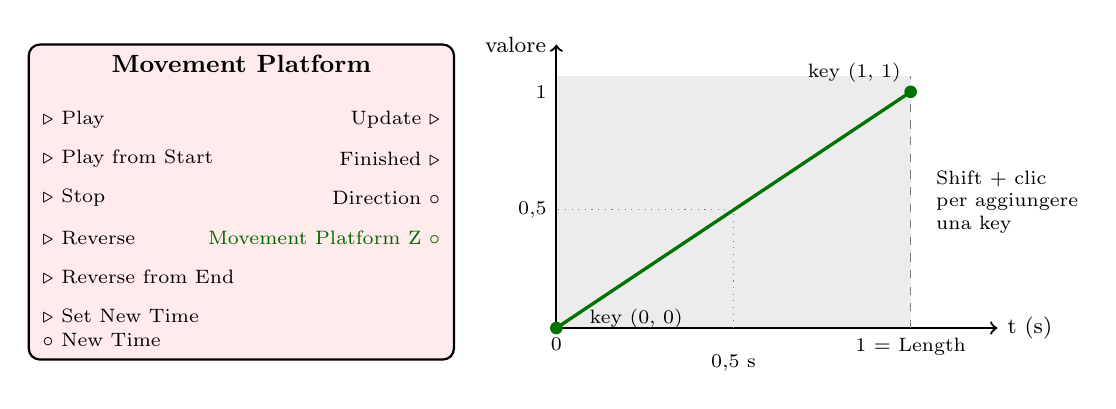
\begin{tikzpicture}[font=\footnotesize,
  ue6tl/.style={draw, thick, rounded corners=4pt, fill=red!8, minimum width=5.4cm,
                minimum height=4.0cm},
  ue6pin/.style={font=\scriptsize}]
  % nodo
  \node[ue6tl] (tl) at (0,0) {};
  \node[font=\small\bfseries] at (0,1.75) {Movement Platform};
  \foreach \t [count=\k] in {Play, Play from Start, Stop, Reverse, Reverse from End,
                             Set New Time} {
    \node[ue6pin, anchor=west] at (-2.65,1.55-0.5*\k) {$\triangleright$ \t};
  }
  \node[ue6pin, anchor=west] at (-2.65,-1.75) {$\circ$ New Time};
  \node[ue6pin, anchor=east] at (2.65,1.05) {Update $\triangleright$};
  \node[ue6pin, anchor=east] at (2.65,0.55) {Finished $\triangleright$};
  \node[ue6pin, anchor=east] at (2.65,0.05) {Direction $\circ$};
  \node[ue6pin, anchor=east, text=green!40!black] at (2.65,-0.45) {Movement Platform Z
    $\circ$};
  % curva
  \begin{scope}[xshift=4.0cm, yshift=-1.6cm]
    \fill[gray!15] (0,0) rectangle (4.5,3.2);
    \draw[->, thick] (0,0) -- (5.6,0) node[right]{t (s)};
    \draw[->, thick] (0,0) -- (0,3.6) node[left]{valore};
    \draw[gray, dashed] (4.5,0) -- (4.5,3.2);
    \node[font=\scriptsize, below] at (4.5,0) {1 = Length};
    \node[font=\scriptsize, below] at (0,0) {0};
    \node[font=\scriptsize, left] at (0,3.0) {1};
    \node[font=\scriptsize, left] at (0,1.5) {0,5};
    \draw[very thick, green!45!black] (0,0) -- (4.5,3.0);
    \fill[green!45!black] (0,0) circle (0.08);
    \fill[green!45!black] (4.5,3.0) circle (0.08);
    \node[font=\scriptsize, right] at (0.3,0.12) {key (0, 0)};
    \node[font=\scriptsize, above left] at (4.5,3.0) {key (1, 1)};
    \draw[gray, dotted] (2.25,0) -- (2.25,1.5) -- (0,1.5);
    \node[font=\scriptsize, align=center] at (2.25,-0.45) {0,5 s};
    \node[font=\scriptsize, align=left, anchor=west] at (4.7,1.6) {Shift + clic\\per
      aggiungere\\una key};
  \end{scope}
\end{tikzpicture}
\caption{Il nodo Timeline della piattaforma e la sua float track. A sinistra i sei
ingressi di esecuzione e le uscite: Update, Finished, Direction e il pin della traccia.
A destra la curva: Length 1 secondo (la zona grigia), due key in (0, 0) e (1, 1); a metà
del tempo il valore è a metà. Schema ricostruito.}
\label{ue6:fig:timeline}
\end{figure}

\begin{table}[htbp]
\centering
\small
\begin{tabular}{@{}p{3.4cm}p{10.6cm}@{}}
\toprule
\textbf{Pin} & \textbf{Che cosa fa} \\
\midrule
Play & riprende dal tempo attuale, in avanti \\
Play from Start & torna a 0 e va in avanti \\
Stop & ferma la timeline dove si trova \\
Reverse & riprende dal tempo attuale, all'indietro \\
Reverse from End & salta alla fine e va all'indietro \\
Set New Time & porta la timeline al tempo New Time \\
\midrule
Update & scatta a ogni aggiornamento mentre la timeline scorre \\
Finished & scatta quando la timeline arriva a un estremo (la fine in avanti, l'inizio
all'indietro) \\
Direction & la direzione attuale: Forward o Backward (un'enumerazione,
\emph{ETimelineDirection}) \\
una uscita per traccia & il valore della traccia al tempo attuale (float, vettore,
colore); le Event track hanno invece un'uscita di esecuzione \\
\bottomrule
\end{tabular}
\caption{I pin del nodo Timeline.}
\label{ue6:tab:timeline}
\end{table}

\paragraph{Approfondimento: le timeline secondo Romero e Sewell.} Nel capitolo 6
(\emph{Enhancing Player Abilities}) i due autori usano una timeline per lo
\emph{zoom} del mirino: una float track \emph{Field of View} da 90 a 45 in 0,3 secondi,
collegata dall'Update al nodo \emph{Set Field of View}, con il tasto premuto su Play e il
tasto rilasciato su \textbf{Reverse}, esattamente lo schema che la lezione userà per la
piattaforma che sale e scende. Il libro aggiunge due osservazioni. La prima: le timeline
sono perfette ``per semplici cambi di valore, come la rotazione di una porta''; per
animazioni complesse, di personaggi o cinematiche, Unreal ha il \textbf{Sequencer}. La
seconda (nella tabella che confronta macro, funzioni ed eventi): i nodi Timeline si
possono usare solo nell'\textbf{Event Graph} di un actor, non dentro le funzioni né
dentro le macro, perché, come i Delay, sono azioni che durano nel tempo. Nelle opzioni
in cima all'editor ci sono poi \textbf{Auto Play} (parte da sola al Begin Play),
\textbf{Loop} (ricomincia all'infinito, utile per un'altalena) e \textbf{Use Last
Keyframe} (fa finire la timeline sull'ultima key invece che alla Length). Le key, con il
tasto destro, possono avere interpolazione lineare, costante o \emph{auto} (curva
morbida, con le tangenti): una curva a ``S'' fa partire e arrivare la piattaforma
dolcemente, invece che di colpo.

% ---------------------------------------------------------------------
\section{L'interpolazione lineare e l'alfa}
\label{ue6:sec:lerp}

``Adesso ci servirebbe fare quello che viene chiamato, in informatica e anche su Unreal,
\textbf{interpolazione}.'' C'è una slide: l'\textbf{interpolazione lineare} ``ci dice:
passo da questo punto a questo punto, passandomi per tutti gli intermedi'', con un
\textbf{alfa}.

\paragraph{L'esempio delle animazioni.} ``L'interpolazione è un concetto che possiamo
trovare in tante cose diverse, tra cui le animazioni.'' Per muovere gli arti di un
personaggio si usano le \textbf{ossa}, interne alla \emph{mesh}. Il docente muove il
braccio davanti alla webcam: ``io non è che vedo subito così, pa!, di scatto: passo
proprio da questo a questo''. ``L'interpolazione è il passaggio per tutti i punti
intermedi che mi fa arrivare alla posizione finale.''

\paragraph{L'alfa.} ``Seguitemi bene attentamente, ragazzi.'' Su una linea che va da 0 a
100, l'alfa è ``un \textbf{puntatore} del punto in cui ci troviamo'', espresso da 0 a 1.
Se siamo a 0, l'alfa è 0; se siamo a 100, l'alfa è 1; ``se l'alfa sta a 0,5, ci
troveremo alla sua metà''. Domanda: se siamo a 20? Uno studente: ``0,2''. ``Ottimo. Siamo
a 0,2: l'alfa sarà a 0,2.'' ``Ci sono varie tipologie di interpolazione, ma
l'interpolazione funziona in questo modo'' (figura~\ref{ue6:fig:lerp}).

\begin{figure}[htbp]
\centering
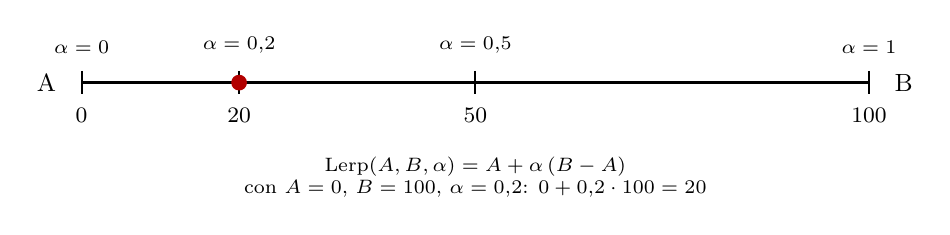
\begin{tikzpicture}[font=\footnotesize]
  \draw[very thick] (0,0) -- (10,0);
  \foreach \x/\l in {0/0, 2/20, 5/50, 10/100} {
    \draw[thick] (\x,0.15) -- (\x,-0.15);
    \node[below] at (\x,-0.2) {\l};
  }
  \node[above, font=\scriptsize] at (0,0.25) {$\alpha = 0$};
  \node[above, font=\scriptsize] at (2,0.25) {$\alpha = 0{,}2$};
  \node[above, font=\scriptsize] at (5,0.25) {$\alpha = 0{,}5$};
  \node[above, font=\scriptsize] at (10,0.25) {$\alpha = 1$};
  \node[left, font=\small] at (-0.2,0) {A};
  \node[right, font=\small] at (10.2,0) {B};
  \fill[red!70!black] (2,0) circle (0.1);
  \node[align=center, font=\scriptsize] at (5,-1.2) {$\mathrm{Lerp}(A, B, \alpha) = A +
    \alpha\,(B - A)$\\con $A = 0$, $B = 100$, $\alpha = 0{,}2$: $0 + 0{,}2 \cdot 100 =
    20$};
\end{tikzpicture}
\caption{L'alfa dell'interpolazione lineare: un numero da 0 a 1 che dice in che punto
del segmento da A a B ci troviamo. L'esempio della lezione: a 20 su 100 l'alfa vale
0,2. La formula, sotto, non è stata scritta a lezione ma è quella che il nodo Lerp
calcola. Schema ricostruito.}
\label{ue6:fig:lerp}
\end{figure}

\paragraph{Approfondimento: Lerp, alfa e timeline.} Il nodo \textbf{Lerp} (per i float)
calcola $A + \alpha(B - A)$: con $\alpha = 0$ restituisce A, con $\alpha = 1$
restituisce B, e in mezzo i valori intermedi in proporzione. Esiste per i vettori
(\textbf{Lerp (Vector)}, che interpola X, Y e Z con lo stesso alfa), per le rotazioni
(\textbf{Lerp (Rotator)}, con l'opzione \emph{Shortest Path}), per i colori e per i
\emph{transform}. L'alfa può anche uscire da $[0, 1]$: con 1,2 il risultato va oltre B
(estrapolazione). Il binomio timeline--Lerp è classico perché divide i compiti: la
\textbf{timeline} decide \emph{come} si scorre nel tempo (quanto dura, con che curva,
avanti o indietro), il \textbf{Lerp} decide \emph{dove} si va (da A a B). Cambiare la
durata o la forma del movimento non tocca A e B, e viceversa. Da non confondere con i nodi
\emph{FInterp To} e \emph{RInterp To} (quest'ultimo usato per la torretta): quelli
avvicinano ogni frame un valore al bersaglio di una frazione, con una velocità e il
Delta Time, senza un alfa né una durata fissa.

% ---------------------------------------------------------------------
\section{Il primo metodo: un Lerp sulla Z}
\label{ue6:sec:metodo1}

``Abbiamo quindi da tirare fuori il nostro bellissimo \textbf{Lerp}.'' Domanda di
partenza, guardando la piattaforma: ``quale asse dovremmo influenzare, che si muova nel
tempo?'' ``La Z.'' ``Ottimo, bravo, Federico.''

\paragraph{La costruzione.} Il docente procede per tentativi, e a un certo punto uno
studente chiede: ``potresti spiegare un po' tutti i passaggi? Perché a un certo punto mi
sono perso''. La versione rispiegata, che è quella da seguire, è questa
(figura~\ref{ue6:fig:metodo1}).
\begin{enumerate}
  \item Si prende il componente \textbf{Platform} e si tira fuori \textbf{Get Relative
        Location}. All'inizio il docente aveva usato Get Actor Location, poi la World
        Location (``scusate, ragazzi, questa è world''), e infine la \emph{relative},
        cioè la posizione rispetto all'actor. Si splitta il vettore.
  \item La \textbf{Z} relativa va, da sola, nel pin \textbf{A} del Lerp: il punto di
        partenza.
  \item La stessa Z più una variabile float nuova, \textbf{MaxHeight}, va nel pin
        \textbf{B}: il punto d'arrivo. Il valore scelto è \textbf{70} (``ci piace 70'';
        ``sono 70 unità sulla Z'').
  \item L'\textbf{Alpha} del Lerp è il pin \textbf{Movement Platform Z} della timeline.
  \item Un \textbf{Make Vector}: X e Y dalla location relativa, invariate; Z dal Lerp.
  \item \textbf{Set Relative Location} sul componente Platform, con il Make Vector nel
        pin \emph{New Location}, eseguito dall'\textbf{Update} della timeline.
\end{enumerate}
La timeline parte dal Begin Overlap della box, attraverso il Branch sul player, con
\textbf{Play}.

\begin{figure}[htbp]
\centering
\begin{tikzpicture}[font=\footnotesize,
  ue6node/.style={draw, thick, rounded corners=4pt, align=center, fill=gray!8,
                  minimum height=0.8cm, text width=2.1cm},
  ue6event/.style={ue6node, fill=red!12},
  ue6exec/.style={-{Stealth[length=2.5mm]}, very thick, black!80},
  ue6data/.style={-{Stealth[length=2mm]}, thick, green!45!black},
  ue6vec/.style={-{Stealth[length=2mm]}, thick, yellow!50!black}]
  \node[ue6event, text width=2.5cm] (ov) at (0,0) {\textbf{On Component Begin
    Overlap} (Box)};
  \node[ue6node, text width=2.4cm] (eq) at (0,-1.8) {Other Actor \textbf{==}\\\textbf{Get
    Player Pawn}};
  \node[ue6node, text width=1.3cm] (br) at (3.0,0) {\textbf{Branch}};
  \node[ue6node, text width=2.3cm] (tl) at (5.8,0) {\textbf{Timeline}\\Movement
    Platform};
  \node[ue6node, text width=2.4cm] (set) at (11.0,0) {\textbf{Set Relative
    Location}\\(Platform)};
  \node[ue6node, text width=2.5cm] (grl) at (3.0,-3.6) {Platform $\rightarrow$
    \textbf{Get Relative Location} (split)};
  \node[ue6node, text width=1.8cm] (mh) at (5.8,-3.6) {Z +\\\textbf{MaxHeight} (70)};
  \node[ue6node, text width=1.4cm] (lerp) at (8.2,-2.0) {\textbf{Lerp}\\A, B, Alpha};
  \node[ue6node, text width=1.7cm] (mv) at (11.0,-2.0) {\textbf{Make Vector}};
  \draw[ue6exec] (ov) -- (br);
  \draw[ue6exec] (br) -- node[above, font=\scriptsize]{True} node[below,
    font=\scriptsize]{Play} (tl);
  \draw[ue6exec] (tl) -- node[above, font=\scriptsize]{Update} (set);
  \draw[-{Stealth[length=2mm]}, thick, red!60!black] (eq.north) -- node[right,
    font=\scriptsize]{bool} (br.south west);
  \draw[ue6data] (tl.south) -- node[left, font=\scriptsize, pos=0.3]{Z track} (lerp.west);
  \draw[ue6data] (grl.north) |- node[pos=0.25, left, font=\scriptsize]{Z $\rightarrow$ A}
    ([yshift=-0.2cm]lerp.west);
  \draw[ue6data] (grl) -- (mh);
  \draw[ue6data] (mh.east) -| node[pos=0.7, right, font=\scriptsize]{B} (lerp.south);
  \draw[ue6data] (lerp) -- node[above, font=\scriptsize]{Z} (mv);
  \draw[ue6data] (grl.south) -- ++(0,-0.35) -| node[pos=0.25, below,
    font=\scriptsize]{X, Y} (mv.south);
  \draw[ue6vec] (mv) -- node[right, font=\scriptsize]{New Location} (set);
\end{tikzpicture}
\caption{Il primo metodo. Il Begin Overlap della box, se l'actor è il player, fa
partire la timeline; a ogni Update un Lerp tra la Z relativa attuale (A) e la stessa Z
più MaxHeight (B), con la traccia della timeline come alfa, diventa la nuova Z della
Platform. Funziona, ma ha un difetto: A e B vengono riletti a ogni Update dalla posizione
già spostata (vedi l'approfondimento). Schema ricostruito.}
\label{ue6:fig:metodo1}
\end{figure}

\paragraph{``Va altissimo''.} In Play la piattaforma sale, ma molto più di 70 unità: a uno
studente, con 70, ``arriva in cielo''; con 30 arriva ``poco più alto del muretto'' della
scena. ``Non so perché, però sia così diverso.'' Il docente promette un metodo ``un po'
più carino e più malleabile''; la spiegazione arriva, in parte, dopo la pausa: ``stiamo
sommando'' (sezione~\ref{ue6:sec:playrate}).

\paragraph{Approfondimento: perché il primo metodo ``somma''.} A ogni Update il grafo
legge la Z \emph{attuale} della Platform, che è già stata spostata dall'Update
precedente, e la usa come A; B è quella Z più 70. Il risultato è quindi
$Z_{\text{nuova}} = Z_{\text{attuale}} + \alpha \cdot 70$: non un punto tra due estremi
fissi, ma un \emph{incremento} che si accumula. Se la timeline si aggiorna $N$ volte in
un secondo, la piattaforma sale di circa $70 \cdot \sum \alpha_k \approx 70 \cdot N/2$
unità: con 60 aggiornamenti al secondo, più di duemila, non settanta. Da qui tre
conseguenze, tutte osservate a lezione. La salita dipende dal \emph{frame rate} (``è la
mia impressione che vada più in alto'': su un computer più veloce, più somme). Rallentare
la timeline con il play rate fa \emph{più} somme, e la piattaforma sale ancora di più;
accelerarla ne fa meno. E con il Reverse il calcolo non torna simmetrico: lo studente
che si vedeva la piattaforma ``sempre leggermente più in basso fino a scomparire sotto il
terreno'' stava osservando proprio l'errore che si accumula a ogni salita e discesa. La
cura è leggere A e B \emph{una volta sola}, prima che la timeline parta, e tenerli fissi:
è il secondo metodo.

% ---------------------------------------------------------------------
\section{La pausa e il Nintendo Direct}
\label{ue6:sec:pausa}

``Sono le 17:37. Facciamo la pausa classica di 20 minuti''; si torna ``alle 18''. Durante
la pausa il docente aiuta uno studente con la foto del codice mandata su Discord (il
problema è l'altezza della piattaforma con il primo metodo: ``70 è giusto'', il resto
``credo sia tutto giusto''), e poco prima della ripresa arrivano le notizie dal
\emph{Nintendo Direct}, riferite da uno studente ``referente''. Nella trascrizione,
molto storpiata, si riconoscono un \emph{remake} di \emph{Ocarina of Time} (``l'Opera of
Time Remake''), un nuovo \emph{Xenoblade}, un \emph{Final Fantasy} in 2D-HD ``stile
\emph{Octopath Traveler}'' e del materiale nuovo su \emph{Deltarune}; il tutto è riportato
come lo si legge nella trascrizione, senza verifiche. La chiacchierata scivola su
\emph{Kingdom Hearts} e sulla trilogia \emph{remake} di \emph{Final Fantasy VII} (``uscirà
prima l'intera trilogia remake''), e su Tetsuya Nomura (``le nomurate''). ``Comunque,
sempre belli questi siparietti'', dice il docente; chi segue in differita può
partecipare alla conversazione su Discord, ``pacificamente''.

% ---------------------------------------------------------------------
\section{La velocità della timeline: Set Play Rate e Duration}
\label{ue6:sec:playrate}

``Allora riprendiamo la nostra bellissima \emph{elevator}, o piattaforma, quello che
vogliamo.'' Una cosa che si può controllare è il \textbf{play rate}: ``la velocità in cui
essa, sempre ripetendo un secondo, viene detta: vai a due volte la tua velocità, a metà
della tua velocità''.

\paragraph{La timeline è un componente.} ``Se avete notato'', nel pannello
\textbf{Components} del Blueprint, accanto a Box, Platform e DefaultSceneRoot, c'è anche
\textbf{Movement Platform}: ``lo stesso nome della timeline''. Ogni timeline aggiunta
crea un componente con il suo nome, e da quel componente si possono chiamare le sue
funzioni. Trascinandolo nel grafo (``Ctrl per il Get''), se ne tira fuori \textbf{Set
Play Rate}, con il \emph{Target} sulla timeline.

\paragraph{Play rate e lunghezza.} Sul \textbf{Begin Play}, Set Play Rate a 0,5: ``la
sua velocità sarà la metà''; a 2, ``il doppio''; a 1, ``andrà come prima''. Il docente
insiste: ``il play rate \textbf{non è la lunghezza}, non è la Length, è diversa''. La
Length dice quanto è lunga la curva; il play rate dice quanto velocemente la si
percorre.

\paragraph{Il primo metodo non regge.} Con il play rate cambiato, la piattaforma del primo
metodo si comporta in modo strano, e il docente ne dà la spiegazione: ``stiamo
aumentando di 30 a ogni frame del nostro secondo''; ``se riduciamo il play rate, lui
sarà più veloce, ma di conseguenza farà meno somme''. Detto meglio: con un play rate più
alto la timeline finisce prima, fa meno Update, e quindi meno somme; con uno più basso ne
fa di più. ``Vedete che non si ferma a quell'unità, perché in questo caso stiamo sommando
solamente: se finisce prima, vuol dire che finirà prima.''

\paragraph{La variabile Duration.} Ragionare in velocità relative è scomodo; è più
naturale dire ``voglio che duri 2 secondi''. Una variabile float \textbf{Duration} e un
piccolo calcolo:
\[
  \text{Play Rate} = \frac{1}{\text{Duration}} \times \text{Timeline Length},
\]
con \textbf{Divide} (``lo slash'') e \textbf{Get Timeline Length} (dal componente della
timeline) moltiplicati con \textbf{Multiply}, e il risultato nel Set Play Rate del Begin
Play. Con Duration 1 e una Length di 1 il play rate è 1, ``velocità normale''. Con
Duration 2 il docente prima dice ``il doppio'', poi si corregge: ``no, scusa, sarà più
lunga, perdonate''; con 0,5 sarà più veloce. È ``una variabile d'appoggio'' che traduce
una durata in secondi nel play rate giusto. Per il resto della lezione la Duration resta
a 1, ``così almeno siamo tranquilli''.

\paragraph{Approfondimento: perché la formula funziona.} Una timeline di lunghezza $L$
percorsa con play rate $r$ dura $L / r$ secondi. Volendo che duri $D$ secondi, basta
porre $L / r = D$, cioè $r = L / D$: è la formula del docente, scritta come $1/D \times
L$. Moltiplicare per la Length rende il calcolo indipendente dalla curva: se un giorno la
timeline diventa lunga 3 secondi, la Duration continua a dire la durata vera. Due
cautele. Una Duration a 0 produce una divisione per zero, e la timeline non si muove più
(il primo sospetto, a lezione, quando la piattaforma di uno studente ``ha smesso di
muoversi''). E il Set Play Rate va chiamato sulla timeline \emph{giusta}: è l'errore
della sezione~\ref{ue6:sec:timelinesbagliata}.

% ---------------------------------------------------------------------
\section{Il secondo metodo: il Billboard e le posizioni salvate}
\label{ue6:sec:metodo2}

Per avere ``due punti specifici da raggiungere, in modo non dipendente da dei valori'',
il docente rifà il grafo. Il vecchio si può tenere, staccato, e copiare (``Ctrl+C,
Ctrl+V'') i pezzi che servono; il Set Relative Location della Platform resta: ``non lo
cancellate, perché è giusto che sia così''.

\paragraph{Il Billboard.} Si aggiunge (\emph{Add}) un componente \textbf{Billboard}:
``un oggetto di questo tipo: è questo \textbf{dinosauro}''. ``Fondamentalmente è un punto
nello spazio'', come lo \emph{Scene Component} già usato per la torretta; ``la
differenza è che ha un'immagine'', visibile solo nell'editor. Il piano: ``prendere la sua
posizione nello spazio, e dire: \emph{lerpami} da questa posizione della piattaforma
iniziale a questa posizione del billboard''. Il Billboard si mette a \textbf{500} sulla
Z (``o di più? 700? Mettete 500, la metà è giusta'').

\paragraph{Lerp (Vector).} Al posto del Lerp sui float, un \textbf{Lerp (Vector)} (``un
v-lerp, un lerp tra vettori''): ``invece che tra due numeri, due float, tra due
vettori''. A è la \textbf{Get Relative Location} della Platform, B quella del Billboard,
l'Alpha la traccia della timeline; l'uscita va direttamente nel Set Relative Location
della Platform, senza Make Vector.

\paragraph{``C'è qualcosa di sbagliato?''} Così com'è, avverte il docente, il grafo ha
ancora il difetto del primo metodo: ``non salviamo mai la posizione delle due''. Se il
Billboard fosse \textbf{attaccato} alla Platform, ``si muoverà insieme ad essa'', e
allora ``avremo un effetto infinito'': la piattaforma insegue un bersaglio che si
allontana, ``un continuo movimento sempre in alto, sempre in alto, pom pom pom''. Il
docente lo mostra riattaccando il Billboard: ``e si ricomincia''. La cura:
\begin{enumerate}
  \item i due Get Relative Location si spostano sul \textbf{Begin Play};
  \item sul pin di uscita di ciascuno, \textbf{Promote to Variable}: la Platform diventa
        \textbf{StartLocation}, il Billboard \textbf{FinishLocation};
  \item nel Lerp (Vector) entrano i \emph{Get} delle due variabili: StartLocation in A,
        FinishLocation in B.
\end{enumerate}
``Così facendo abbiamo delle variabili che sono sempre fisse'': ``sarà sempre la stessa
posizione'' (figura~\ref{ue6:fig:metodo2}).

\paragraph{Il bello del Billboard.} ``La cosa bella, poi, che possiamo vedere con questo
metodo'': il dinosauro si può spostare nello spazio, nei dettagli della piattaforma, e la
piattaforma raggiungerà quel punto. ``Dovete fare un livello? L'avete alzato a 8 metri?
Prendete il billboard, lo mettete a 800'': ``devo arrivare qua sopra, quindi arriverò
qua. Ecco fatto, sono arrivato preciso''. (``Salto, l'ho mancato malissimo.'') E non solo
in verticale: spostando il Billboard anche sulla X o sulla Y, ``andrà in diagonale'';
``potremmo pure fare piattaforme in orizzontale, in diagonale, come vi pare''. ``Invece
di fare matematica'', si prendono direttamente i due vettori.

\paragraph{Il ritorno: Reverse.} Scendendo dalla piattaforma, questa ``rimane là''.
``Vi potrei dire: facciamo una nuova timeline e la facciamo al contrario. Non serve.
Perché abbiamo \textbf{Reverse}.'' L'\textbf{On Component End Overlap} della box,
collegato al pin Reverse della timeline: ``esco fuori e lei se ne torna al suo posto'',
perché ``invece di fare da A a B, fa da B ad A. Questo è insito nella timeline''.

\begin{figure}[htbp]
\centering
\begin{tikzpicture}[font=\footnotesize,
  ue6node/.style={draw, thick, rounded corners=4pt, align=center, fill=gray!8,
                  minimum height=0.8cm, text width=2.1cm},
  ue6event/.style={ue6node, fill=red!12},
  ue6var/.style={ue6node, fill=blue!10, rounded corners=8pt},
  ue6exec/.style={-{Stealth[length=2.5mm]}, very thick, black!80},
  ue6data/.style={-{Stealth[length=2mm]}, thick, green!45!black},
  ue6vec/.style={-{Stealth[length=2mm]}, thick, yellow!50!black}]
  % Begin Play
  \node[ue6event, text width=2.4cm] (bp) at (0,0) {\textbf{Event Begin Play}};
  \node[ue6node, text width=2.3cm] (s1) at (3.3,0) {\textbf{Set}\\StartLocation};
  \node[ue6node, text width=2.3cm] (s2) at (6.4,0) {\textbf{Set}\\FinishLocation};
  \node[ue6node, text width=2.2cm] (pr) at (9.6,0) {\textbf{Set Play Rate}\\($1/D \times
    L$)};
  \node[ue6node, text width=2.5cm] (g1) at (3.3,-1.6) {Platform $\rightarrow$ Get
    Relative Location};
  \node[ue6node, text width=2.5cm] (g2) at (6.4,-1.6) {Billboard $\rightarrow$ Get
    Relative Location};
  \draw[ue6exec] (bp) -- (s1);
  \draw[ue6exec] (s1) -- (s2);
  \draw[ue6exec] (s2) -- (pr);
  \draw[ue6vec] (g1) -- (s1);
  \draw[ue6vec] (g2) -- (s2);
  % overlap e timeline
  \begin{scope}[yshift=-3.6cm]
    \node[ue6event, text width=2.6cm] (bo) at (-0.2,0) {\textbf{Begin Overlap}
      (Box)\\+ Branch sul player};
    \node[ue6event, text width=2.6cm] (eo) at (-0.2,-1.5) {\textbf{End Overlap} (Box)};
    \node[ue6node, text width=2.2cm, minimum height=2.2cm] (tl) at (3.6,-0.75)
      {\textbf{Timeline}\\Movement\\Platform};
    \node[ue6node, text width=1.9cm] (lv) at (7.0,-2.5) {\textbf{Lerp (Vector)}\\A, B,
      Alpha};
    \node[ue6var, text width=1.9cm] (v1) at (7.0,-4.0) {StartLocation};
    \node[ue6var, text width=2.1cm] (v2) at (9.8,-4.0) {FinishLocation};
    \node[ue6node, text width=2.4cm] (set) at (10.4,-0.4) {\textbf{Set Relative
      Location}\\(Platform)};
    \draw[ue6exec] (bo.east) -- node[above, font=\scriptsize]{Play} ([yshift=0.75cm]tl.west);
    \draw[ue6exec] (eo.east) -- node[below, font=\scriptsize]{Reverse}
      ([yshift=-0.75cm]tl.west);
    \draw[ue6exec] ([yshift=0.35cm]tl.east) -- node[above, font=\scriptsize]{Update}
      (set.west);
    \draw[ue6data] ([yshift=-0.6cm]tl.east) -| node[pos=0.25, above,
      font=\scriptsize]{Alpha} (lv.north);
    \draw[ue6vec] (v1) -- node[left, font=\scriptsize]{A} (lv);
    \draw[ue6vec] (v2.north) |- node[pos=0.25, right, font=\scriptsize]{B} (lv.east);
    \draw[ue6vec] (lv.east) -- ++(0.9,0) |- node[pos=0.2, right,
      font=\scriptsize]{New Location} (set.south west);
  \end{scope}
\end{tikzpicture}
\caption{Il secondo metodo. Sopra: al Begin Play le posizioni relative della Platform e
del Billboard vengono salvate una volta per tutte in StartLocation e FinishLocation (con
Promote to Variable), e si imposta il play rate dalla Duration. Sotto: il Begin Overlap
fa Play, l'End Overlap fa Reverse; a ogni Update un Lerp (Vector) tra i due punti fissi,
con la traccia come alfa, diventa la nuova posizione della Platform. Schema
ricostruito.}
\label{ue6:fig:metodo2}
\end{figure}

\paragraph{I problemi.} ``Problemi su questo? Siete a posto?'' Tre casi.
\begin{itemize}
  \item \textbf{``A me non si muove.''} Il docente ripassa la lista: le due Get Relative
        Location, le due variabili, la timeline in Play, l'Update, il Lerp tra i
        vettori, l'Alpha collegato. Lo studente non aveva capito come creare le
        variabili: tasto destro sul pin, \textbf{Promote to Variable}, e il nome. Poi
        StartLocation in A, FinishLocation in B, e l'Alpha alla traccia della timeline.
  \item \textbf{L'evento diventato Custom Event.} Uno studente scopre da solo il suo
        errore: copiando e incollando il blocco, l'evento di overlap ``mi ha preso come
        Custom Event generico, e quindi non si muoveva''. Un evento di componente
        incollato in un Blueprint perde il legame con il componente e diventa un evento
        qualunque, che nessuno chiama. ``Errore di distrazione.''
  \item \textbf{Ero rimasto indietro.} Uno studente, che aveva ricevuto una telefonata,
        riceve il riassunto: Billboard, Get Relative Location della Platform in
        StartLocation e del Billboard in FinishLocation, il Lerp (Vector) con l'alfa, il
        Set Relative Location, e il Reverse sull'End Overlap.
\end{itemize}

\paragraph{Approfondimento: Billboard figlio di chi?} Il docente fa vedere che, con il
Billboard attaccato alla Platform, la piattaforma ``sale all'infinito'', e che salvando le
posizioni al Begin Play il problema scompare. Ma c'è un dettaglio che la lezione non
esplicita: se il Billboard resta figlio della Platform, la sua \emph{relative location}
è relativa alla Platform, non all'actor; salvarla al Begin Play dà $(0, 0, 500)$ rispetto
alla piattaforma, mentre il Set Relative Location della Platform lavora rispetto alla
radice dell'actor. I due numeri coincidono solo se la Platform sta nell'origine
dell'actor (come nel Blueprint della lezione). La configurazione più robusta è mettere il
Billboard come figlio della \textbf{DefaultSceneRoot}, accanto alla Platform, così che
le due posizioni relative siano nello stesso spazio e il bersaglio non si muova mai con
la piattaforma. Un'altra soluzione, equivalente, è salvare e impostare le posizioni nel
mondo (Get e Set World Location). Infine: il ``dinosauro'' è visibile solo nell'editor;
nel gioco il Billboard non si vede, come tutti i componenti di servizio.

% ---------------------------------------------------------------------
\section{La timeline sbagliata}
\label{ue6:sec:timelinesbagliata}

Il docente vuole far vedere che la Duration funziona anche con il secondo metodo: ``la
cambio in 2''; poi, ``mettiamo dei valori che posso riconoscere, tipo 10''. Ma la
velocità non cambia. ``Non mi setta il play rate, forse.'' Anche a uno studente,
``l'unica cosa è la duration: non va effettivamente a modificare la velocità''. Il
docente prova un Print, un play rate a 0,1, a mille: ``sempre lo stesso''.

\paragraph{La soluzione, da uno studente.} ``Domanda un po' stupida: non è che forse
l'attore deve essere Platform e non Movement Platform?'' Non è quello, ma è la pista
giusta: ``errore mio''. Il secondo metodo usa una timeline \emph{nuova}, che si chiama
semplicemente \textbf{Timeline}; il Set Play Rate del Begin Play aveva come Target ancora
\textbf{Movement Platform}, ``quella dell'esempio di prima''. ``Stavamo referenziando la
timeline dell'altro esempio, e non la playavamo mai.''

\paragraph{La lezione dell'errore.} ``Da questo errore possiamo imparare qualche cosa'':
``le timeline hanno un \textbf{nome}''. Ogni timeline è un componente distinto, e le sue
funzioni (Set Play Rate, Get Timeline Length, Play, Reverse\ldots) agiscono solo su di
lei. Con il Target giusto e una Duration di 3, la piattaforma ``adesso è più lenta,
perché dura di più''. Morale: dare alle timeline nomi chiari, e cancellare quelle che non
servono più.

% ---------------------------------------------------------------------
\section{L'audio: la Sound Cue}
\label{ue6:sec:cue}

``Se non ci sono più problemi, passiamo al nostro bellissimo \emph{sound}.''

\paragraph{Importare il file.} Un consiglio d'ordine: una \textbf{cartella audio} nel
Content Browser (tasto destro, \emph{New Folder}). Per importare il file scaricato da
Discord basta \textbf{trascinarlo} nel Content Browser: appare un asset ``con la linea'',
una \textbf{Sound Wave}, senza altre domande.

\paragraph{Creare la Cue.} Sulla Sound Wave, tasto destro, \textbf{Create Cue} (``è il
secondo''). La \textbf{Sound Cue} (``la queue'', ``la Q'', nella trascrizione) è, dice il
docente, ``un \emph{sound} programmabile, tra virgolette''. Doppio clic: si apre un grafo
``come abbiamo visto anche su Unreal molto spesso'', con un nodo \textbf{Wave Player}
(il nostro suono) collegato all'\textbf{Output}. A sinistra, i dettagli della Cue:
\textbf{Volume Multiplier}, \textbf{Pitch Multiplier}, \emph{Sound Class} (``class
override''), \emph{Attenuation} e così via, ``tutti i vari dati che possiamo
modificare''.

\paragraph{Il pitch.} Con il Pitch Multiplier a 2 il suono è più alto; a 0,5 ``è pitchato
verso il basso'': ``molto più basso livello di tono, e anche più lento''. ``Perché il
pitch influenza sia la velocità sia la tonalità.'' Si torna a 1.

\paragraph{Il loop.} Con Play il suono parte ``solo una volta''; ``noi vogliamo che vada
in loop'' finché la piattaforma si muove, ``tipo: pipi, pipi, pipi''. Sul nodo
\textbf{Wave Player} si spunta \textbf{Looping}. (``Ovviamente rompe'': con la barra
spaziatrice si avvia e si interrompe l'anteprima.)

\paragraph{Il Modulator.} ``Vogliamo che magari il pitch o il volume siano un valore
\textbf{randomico}, tra un valore e un altro, in modo che non sia sempre lo stesso
suono.'' Si inserisce un nodo \textbf{Modulator} tra il Wave Player e l'Output: ha
\textbf{Pitch Min}, \textbf{Pitch Max}, \textbf{Volume Min} e \textbf{Volume Max}. I
valori della lezione: pitch tra \textbf{1,7} e \textbf{2}, volume tra \textbf{1} e
\textbf{1,2}. A ogni riproduzione il suono è ``leggermente più basso, leggermente più
alto''. Il perché, con il gioco della palla del docente: quando rimbalza fa un
\emph{boing}, ``e visto che avevo solo un suono'', che ripetuto ``sembra la stessa
cosa'', un pitch minimo e massimo hanno dato ``un risultato molto più gradevole''.

\paragraph{Il Random.} ``Esiste anche il \textbf{Random}'': se si hanno più suoni, il
nodo Random ne sceglie uno a caso a ogni riproduzione. Il docente lo prova mettendo nel
Random due rami, uno con il Modulator e uno senza, e ascoltando quale esce. L'uso tipico:
``un proiettile che prende un muro: invece di avere sempre lo stesso suono, mettete tutti
e tre i suoni nel Random''. Per la piattaforma non serve, e si torna al solo Modulator
(figura~\ref{ue6:fig:cue}).

\begin{figure}[htbp]
\centering
\begin{tikzpicture}[font=\footnotesize,
  ue6snode/.style={draw, thick, rounded corners=4pt, align=center, fill=violet!10,
                   minimum height=1.0cm, text width=2.5cm},
  ue6out/.style={draw, thick, rounded corners=4pt, align=center, fill=gray!20,
                 minimum height=1.0cm, text width=1.6cm},
  ue6aud/.style={-{Stealth[length=2.5mm]}, very thick, violet!60!black}]
  \node[ue6snode] (wp) at (0,0) {\textbf{Wave Player}\\SFX Moving Platform\\Looping
    \checkmark};
  \node[ue6snode] (mod) at (4.0,0) {\textbf{Modulator}\\Pitch 1,7--2\\Volume 1--1,2};
  \node[ue6out] (out) at (7.6,0) {\textbf{Output}};
  \draw[ue6aud] (wp) -- (mod);
  \draw[ue6aud] (mod) -- (out);
  \node[draw, dashed, rounded corners=4pt, align=left, text width=4.6cm, font=\scriptsize]
    at (11.4,0) {dettagli della Cue: Volume Multiplier, Pitch Multiplier (1), Sound
    Class, Attenuation\ldots};
  % variante random
  \begin{scope}[yshift=-2.4cm]
    \node[ue6snode, text width=2.0cm] (w1) at (0,0.6) {Wave Player 1};
    \node[ue6snode, text width=2.0cm] (w2) at (0,-0.6) {Wave Player 2};
    \node[ue6snode, text width=1.6cm] (rnd) at (4.0,0) {\textbf{Random}};
    \node[ue6out] (out2) at (7.6,0) {\textbf{Output}};
    \draw[ue6aud] (w1.east) -- (rnd.west);
    \draw[ue6aud] (w2.east) -- (rnd.west);
    \draw[ue6aud] (rnd) -- (out2);
    \node[align=left, font=\scriptsize, text width=4.6cm] at (11.4,0) {variante: più
      suoni, uno scelto a caso a ogni riproduzione (l'esempio del proiettile contro il
      muro)};
  \end{scope}
\end{tikzpicture}
\caption{La Sound Cue della piattaforma: il Wave Player in loop, un Modulator che varia
a caso pitch e volume a ogni riproduzione, l'Output. Sotto, la variante con il nodo
Random mostrata a lezione e poi scartata. Schema ricostruito.}
\label{ue6:fig:cue}
\end{figure}

\paragraph{Approfondimento: Sound Wave, Sound Cue, MetaSound.} La \textbf{Sound Wave} è
il file audio importato, con poche proprietà proprie (fra cui un suo \emph{Looping}). La
\textbf{Sound Cue} è un piccolo grafo che combina una o più Wave con nodi di
elaborazione: Modulator, Random, \emph{Mixer}, \emph{Concatenator}, \emph{Delay},
\emph{Attenuation}\ldots; nei Blueprint si può passare indifferentemente una Wave o una
Cue a qualunque nodo che vuole un \emph{Sound}. In Unreal Engine 5 esistono anche i
\textbf{MetaSound}, un sistema più recente e più potente, che genera e manipola l'audio
con un grafo simile a quello dei Blueprint; le Sound Cue restano supportate e sono il
punto di partenza più semplice. Il formato \textbf{WAV} raccomandato dal docente è quello
standard per l'import: non compresso, lo comprime poi l'engine secondo la piattaforma.
Sul pitch, l'osservazione del docente è esatta: in una Sound Cue il Pitch Multiplier
cambia la velocità di riproduzione, quindi alza o abbassa il tono e accorcia o allunga il
suono insieme, come un disco suonato a giri sbagliati.

% ---------------------------------------------------------------------
\section{Far suonare la piattaforma: Spawn Sound, Do Once e Stop}
\label{ue6:sec:suono}

``Abbiamo due modi per piazzare i suoni'': i nodi \textbf{Play Sound 2D} e \textbf{Play
Sound at Location}, e i nodi \textbf{Spawn Sound 2D} e \textbf{Spawn Sound at Location}.
``La differenza sostanziale è che uno \emph{playa} il suono solamente; l'altro lo
\emph{spawna}, e quindi crea una \textbf{referenza}'', come lo Spawn Actor from Class
``che quando spawna ha un Return Value''.

\paragraph{La prova con Play Sound 2D.} ``Proviamo a mettere Play Sound 2D'': la Cue
nel pin Sound, l'esecuzione dall'Update della timeline. Il docente sale sulla piattaforma: il suono parte,
``e non smette più''. Peggio: l'Update scatta a ogni aggiornamento, quindi i suoni si
sovrappongono (``come avete sentito, è stato uno stormo di uccelli incredibile''). Due
problemi, due soluzioni.
\begin{itemize}
  \item Il suono è in loop: per fermarlo bisogna sapere \emph{quale} suono fermare, e il
        Play Sound non lo dice. Serve lo \textbf{Spawn Sound at Location}, che
        restituisce la referenza.
  \item L'Update scatta molte volte: serve un \textbf{Do Once}, ``che lo fa una sola
        volta''.
\end{itemize}

\paragraph{Lo spawn.} \textbf{Do Once}, poi \textbf{Spawn Sound at Location}: Sound la
Cue, Location la \textbf{Get Actor Location} (``alla locazione dell'attore playerà questo
suono''; il docente pensa prima alla piattaforma, poi sceglie l'actor). Dal \textbf{Return
Value}, \textbf{Promote to Variable}: \textbf{SoundPlatform}. ``Adesso, di questo suono
che abbiamo creato, abbiamo la referenza: qualcosa che punta e ci dice: ehi, questo è il
suono che fa pipipipi.''

\paragraph{Lo stop.} ``Io voglio che si fermi quando la timeline finisce'', cioè quando
arriva in cima (a 1) o torna alla base (a 0). Sul \textbf{Finished} della timeline: Get
di SoundPlatform, \textbf{Stop}. ``Fino a che non è arrivato in cima, o fino a che non è
tornato alla base, il suono playerà, e si stopperà appena finisce la timeline.''

\paragraph{Il Reset del Do Once.} ``Un'ultima cosa molto importante.'' Il Do Once, una
volta passato, resta chiuso; ha però un ingresso \textbf{Reset}: ``se lo inserisco là
dentro, questo Do Once si resetta, si apre, e dà la possibilità di essere rieseguito''.
``Quando ho stoppato il suono una volta, lo devo riattivare per la volta dopo'': dopo lo
Stop, il Reset. ``E si ferma; scendo, ed eccolo. Benissimo.''

% ---------------------------------------------------------------------
\section{Il pitch che cambia con la direzione}
\label{ue6:sec:pitch}

``Potremmo anche, ipoteticamente\ldots'' L'idea: un suono \textbf{più alto quando la
piattaforma sale} e \textbf{più basso quando scende}. Il componente audio spawnato ha la
funzione \textbf{Set Pitch Multiplier}, da chiamare sulla referenza SoundPlatform.

\paragraph{Come sapere se sale o scende.} Il docente comincia a ragionare con un Branch
(``se sta andando da StartLocation a FinishLocation\ldots''), poi si ferma: ``possiamo
usare una cosa molto interessante''. Il pin \textbf{Direction} della timeline è
un'\textbf{enumerazione} (``che vedremo in seguito che cos'è, ma oggi ci serve
semplicemente vedere questa cosa''): ``una variabile che ha dentro di sé due elementi'',
\emph{Forward} e \emph{Backward}. Tirandone fuori uno \textbf{Switch on
ETimelineDirection} si ottengono due uscite di esecuzione: ``avanti vuol dire che sta
andando 0--1, e indietro è 1--0''.
\begin{itemize}
  \item \textbf{Forward}: Set Pitch Multiplier su SoundPlatform a \textbf{1}, il pitch
        normale;
  \item \textbf{Backward}: Set Pitch Multiplier a \textbf{0,4}, ``per far puh, puh, puh,
        un po' più bassino: una discesa'' (il docente prova anche 0,5 e 0,1, ``molto
        basso''; il valore finale è 0,4).
\end{itemize}
``Mettiamo tutto nel Do Once'' (figura~\ref{ue6:fig:suono}).

\paragraph{L'errore dell'ordine.} A una studentessa il grafo, ``sulla carta'', è giusto,
ma il compilatore segnala un errore: il Set Pitch Multiplier dice che il suono ``non è
mai stato creato''. Il motivo è l'ordine: lo Switch, con i due Set Pitch Multiplier,
veniva eseguito \emph{prima} che lo Spawn Sound avesse riempito la variabile, quindi su
una referenza vuota. ``Metti prima il Do Once'', e dopo lo spawn e il Set della
variabile, lo Switch con i due rami. ``Dovrebbe andare.'' E va (dopo aver condiviso anche
l'audio del computer su Zoom, per farlo sentire).

\begin{figure}[htbp]
\centering
\begin{tikzpicture}[font=\footnotesize,
  ue6node/.style={draw, thick, rounded corners=4pt, align=center, fill=gray!8,
                  minimum height=0.8cm, text width=2.0cm},
  ue6var/.style={ue6node, fill=blue!10, rounded corners=8pt},
  ue6exec/.style={-{Stealth[length=2.5mm]}, very thick, black!80},
  ue6data/.style={-{Stealth[length=2mm]}, thick, violet!60!black}]
  \node[ue6node, text width=2.0cm, minimum height=2.0cm] (tl) at (0,0)
    {\textbf{Timeline}};
  \node[ue6node, text width=1.5cm] (do) at (3.4,0.6) {\textbf{Do Once}};
  \node[ue6node, text width=2.4cm] (sp) at (6.1,0.6) {\textbf{Spawn Sound at
    Location}\\Cue, Get Actor Location};
  \node[ue6var, text width=2.1cm] (sv) at (9.1,0.6) {\textbf{Set}\\SoundPlatform};
  \node[ue6node, text width=2.1cm] (sw) at (12.0,0.6) {\textbf{Switch on
    ETimelineDirection}};
  \node[ue6node, text width=2.4cm] (f) at (12.0,2.4) {\textbf{Set Pitch
    Multiplier}\\1 (sale)};
  \node[ue6node, text width=2.4cm] (b) at (12.0,-1.2) {\textbf{Set Pitch
    Multiplier}\\0,4 (scende)};
  \node[ue6node, text width=2.2cm] (st) at (3.4,-1.9) {SoundPlatform $\rightarrow$
    \textbf{Stop}};
  \draw[ue6exec] ([yshift=0.6cm]tl.east) -- node[above, font=\scriptsize]{Update} (do);
  \draw[ue6exec] (do) -- (sp);
  \draw[ue6exec] (sp) -- (sv);
  \draw[ue6exec] (sv) -- (sw);
  \draw[ue6exec] (sw.north) -- node[right, font=\scriptsize]{Forward} (f.south);
  \draw[ue6exec] (sw.south) -- node[right, font=\scriptsize]{Backward} (b.north);
  \draw[ue6exec] ([yshift=-0.6cm]tl.east) -- ++(0.4,0) |- node[pos=0.3, left,
    font=\scriptsize]{Finished} (st.west);
  \draw[ue6exec] (st.north) -- node[left, font=\scriptsize]{Reset} (do.south);
  \draw[ue6data] (tl.south) -- (0,-3.1) -- node[below, font=\scriptsize, pos=0.85]{Direction}
    (10.5,-3.1) |- ([yshift=-0.25cm]sw.west);
  \draw[ue6data] (sp.south) -- ++(0,-0.4) -| node[pos=0.25, below, font=\scriptsize]{Return
    Value} (sv.south);
\end{tikzpicture}
\caption{Il suono della piattaforma. Al primo Update il Do Once lascia passare: lo Spawn
Sound at Location crea il suono in loop, la sua referenza viene salvata in SoundPlatform,
e lo Switch sulla Direction della timeline sceglie il pitch (1 in salita, 0,4 in
discesa). Al Finished, il suono si ferma e il Do Once si riapre per la volta dopo.
Schema ricostruito; l'ordine è quello che risolve l'errore della studentessa (prima lo
spawn, poi il pitch).}
\label{ue6:fig:suono}
\end{figure}

\paragraph{Approfondimento: Play o Spawn, 2D o at Location.} Romero e Sewell (capitolo 6)
usano \textbf{Play Sound at Location} per l'esplosione del bersaglio colpito: un suono
breve, ``spara e dimentica'', che non serve più controllare, con la \emph{Hit Location}
dell'Event Hit come posizione. Per un suono in loop, che va fermato o modificato, serve
invece uno dei nodi \textbf{Spawn Sound}, che creano un \textbf{Audio Component} e ne
restituiscono la referenza: su di esso si chiamano Stop, Set Pitch Multiplier, Set Volume
Multiplier, \emph{Fade Out} e così via. I nodi \textbf{2D} suonano ``in cuffia'', senza
posizione né attenuazione con la distanza (adatti a musica e interfaccia); quelli
\textbf{at Location} suonano in un punto del mondo, e con un'\emph{attenuation} si
sentono di meno allontanandosi. Due osservazioni sulla scelta della lezione. La prima: la
Get Actor Location è la posizione della \emph{radice} dell'actor, che non si muove,
perché a salire è solo la Platform; il suono resta quindi alla base. Per un suono che
segue la piattaforma esiste \textbf{Spawn Sound Attached}, che lo attacca a un componente
(qui, la Platform). La seconda: invece di Do Once e Spawn a ogni salita, si può aggiungere
un \textbf{Audio Component} direttamente ai componenti del Blueprint, con \emph{Auto
Activate} spento, e chiamare \emph{Play} e \emph{Stop} su di esso; la referenza c'è già,
e l'errore dell'ordine non può capitare.

% ---------------------------------------------------------------------
\section{La chiusura}
\label{ue6:sec:chiusura}

``Ci siete voi altri, ragazzi? C'è qualche problema? Funziona tranquillamente?'' ``Adesso
andiamo a cena, siamo a fine lezione.'' L'ultimo invito: ``se ci sono problemi, diteli
ora o tacete per sempre; o almeno fino alla prossima lezione''. L'appuntamento è per
\textbf{giovedì}. ``Vi ringrazio per l'attenzione. Buonasera a tutti, ragazzi. Ciao,
ciao.''

\begin{table}[htbp]
\centering
\small
\begin{tabular}{@{}p{5.4cm}p{8.6cm}@{}}
\toprule
\textbf{Sintomo} & \textbf{Causa e rimedio} \\
\midrule
Pop-up ``project files are not associated'' a ogni avvio del launcher & associazione
dei file di progetto rotta dagli aggiornamenti: Fix Now; i progetti non corrono rischi \\
Il messaggio di overlap non compare & la risposta di uno dei due oggetti è Ignore, o
manca Generate Overlap Events; con Overlap da una parte e Block dall'altra il risultato
è un overlap \\
I cubi si spawnano all'infinito, impilati & il trace sul Tick vede i cubi appena nati:
mesh di BP\_Cube su Custom, Visibility su Ignore (e Always Spawn, Ignore Collisions) \\
Il cubo si può solo scalare & è stato trascinato sopra il DefaultSceneRoot,
sostituendolo: ricrearlo come figlio della radice \\
``Un muro basso'' invece della griglia & cubi troppo grandi per l'intervallo di 100:
rimpicciolire BP\_Cube (0.5, 0.2) \\
Le righe non compaiono & il secondo ciclo usa la X di Get Actor Location invece della X
del primo ciclo, o somma l'offset alla X invece che alla Y \\
Il ciclo calcola ma non esegue & Loop Body non collegato al trace, o il trace non
collegato allo spawn \\
Il trace della riga non si vede & manca l'End (Up Vector $\times\,-5000$ sommato allo
Start) \\
Lag con la matrice & spawn e trace a ogni frame: Set Actor Tick Enabled (falso) sul
Completed del For Loop \\
La box non segue la piattaforma & la Box Collision non è figlia della Platform \\
La piattaforma sale troppo (``arriva in cielo'') & primo metodo: A e B riletti dalla
posizione già spostata, la salita si accumula; usare posizioni salvate (secondo metodo) \\
La piattaforma scende ogni volta un po' di più & stesso errore che si accumula a ogni
Play e Reverse: secondo metodo \\
La piattaforma insegue il Billboard all'infinito & il bersaglio si muove con la
Platform: salvare Start e Finish Location al Begin Play (e il Billboard figlio della
radice) \\
La piattaforma resta su quando si scende & End Overlap non collegato a Reverse \\
La piattaforma non si muove dopo un copia-incolla & l'evento di overlap incollato è
diventato un Custom Event generico: ricrearlo dal componente Box \\
Duration e play rate non hanno effetto & Set Play Rate sulla timeline sbagliata (il
Target è la timeline del primo metodo); o Duration a 0 \\
Il suono non smette più & Play Sound non dà una referenza: Spawn Sound at Location,
Promote to Variable, Stop sul Finished \\
Tanti suoni sovrapposti (``uno stormo di uccelli'') & lo spawn sull'Update scatta a ogni
aggiornamento: Do Once, con Reset dopo lo Stop \\
Il suono parte solo la prima volta & manca il Reset del Do Once \\
Errore su Set Pitch Multiplier (``mai creato'') & il pitch viene impostato prima dello
spawn: prima Do Once, Spawn e Set, poi lo Switch \\
\bottomrule
\end{tabular}
\caption{I problemi incontrati durante la lezione, con la causa e il rimedio.}
\label{ue6:tab:errori}
\end{table}

\begin{table}[htbp]
\centering
\small
\begin{tabular}{@{}p{4.4cm}p{9.6cm}@{}}
\toprule
\textbf{Nodo, componente o impostazione} & \textbf{Che cosa fa} \\
\midrule
Collision Presets / Collision Enabled & configurazioni pronte delle collisioni; attiva o
disattiva query (trace e overlap) e fisica \\
Object Type / Object Responses & la categoria dell'oggetto; come risponde (Ignore,
Overlap, Block) a ciascuna categoria \\
New Object Channel (Project Settings) & crea una nuova categoria di oggetti \\
Event ActorBegin/EndOverlap & inizio e fine di un overlap di un actor \\
On Component Begin/End Overlap & inizio e fine di un overlap di un componente (Other
Actor, Other Comp) \\
For Loop (Completed) & ripete il Loop Body da First a Last Index; Completed scatta alla
fine \\
Sequence & esegue in ordine le sue uscite Then 0, Then 1, \ldots \\
Break Hit Result & scompone l'Out Hit di un trace (Blocking Hit, Location, Impact Point,
Normal, \ldots) \\
Split Struct Pin & separa un pin struttura (un \emph{transform}, un vettore) nei suoi
campi \\
Set Actor Tick Enabled & accende o spegne l'Event Tick di un actor \\
Box Collision & un volume invisibile per overlap e collisioni \\
Billboard & un punto nello spazio con un'icona, visibile solo nell'editor \\
== (Equal) & confronta due valori o referenze; restituisce un booleano \\
Get Player Pawn & la referenza al Pawn controllato dal giocatore \\
Actor Has Tag & vero se l'actor ha il tag indicato \\
Timeline & una linea del tempo con tracce (Float, Vector, Event, Color); Play, Reverse,
Update, Finished, Direction \\
Set Play Rate / Get Timeline Length & velocità di una timeline; la sua lunghezza \\
Lerp / Lerp (Vector) & interpolazione lineare tra A e B con un alfa da 0 a 1 \\
Get / Set Relative Location & posizione di un componente rispetto al suo genitore \\
Make Vector & costruisce un vettore da X, Y, Z \\
Promote to Variable & crea una variabile del tipo di un pin e la imposta \\
Sound Wave / Sound Cue & il file audio importato; il grafo che lo elabora (Wave Player,
Looping, Modulator, Random) \\
Play Sound 2D / at Location & suona un suono e basta, senza referenza \\
Spawn Sound 2D / at Location & crea un Audio Component e ne restituisce la referenza \\
Stop / Set Pitch Multiplier & ferma un Audio Component; ne cambia il pitch \\
Do Once (Reset) & lascia passare l'esecuzione una volta, finché non viene resettato \\
Switch on ETimelineDirection & due uscite: Forward e Backward \\
\bottomrule
\end{tabular}
\caption{I nodi, i componenti e le impostazioni della sesta lezione.}
\label{ue6:tab:nodi}
\end{table}

% ---------------------------------------------------------------------
\section*{Punti chiave del capitolo}
\addcontentsline{toc}{section}{Punti chiave del capitolo}

\begin{itemize}
  \item Le risposte di collisione sono tre: \textbf{Ignore} (nessuna collisione,
        nessun evento), \textbf{Overlap} (gli oggetti si attraversano, ma l'engine
        notifica l'incontro) e \textbf{Block} (collisione fisica e di controllo). Fra due
        oggetti vince la risposta meno restrittiva.
  \item L'\textbf{Object Type} è la categoria di un oggetto; le \textbf{Object Responses}
        dicono come l'oggetto risponde a ogni categoria. Nuovi tipi e nuovi canali si
        creano in \emph{Project Settings $\rightarrow$ Collision}: pochi, uno per ogni
        categoria o domanda diversa, non uno per oggetto.
  \item I \textbf{volumi invisibili} in overlap sono lo strumento classico per far
        scattare eventi (una cutscene, una piattaforma): \textbf{Begin} ed \textbf{End
        Overlap}, a livello di actor o di componente, scattano una volta in entrata e
        una in uscita.
  \item I trace costano: vanno usati per azioni precise (il salto anticipato dei
        platformer) e spenti quando non servono. Gli oggetti di un gioco devono
        restare il più possibile \textbf{isolati}, e comunicare.
  \item La \textbf{matrice di cubi}: un Branch sul trace, \textbf{Spawn Actor from Class}
        di BP\_Cube nella Location del \textbf{Break Hit Result}; un \textbf{Sequence}
        che spawna la colonna e fa partire un secondo \textbf{For Loop} per la riga
        (stessa X, Y crescente). Il cubo deve ignorare il canale Visibility, e alla fine
        \textbf{Set Actor Tick Enabled} spegne il Tick.
  \item La piattaforma: una Static Mesh, una \textbf{Box Collision} figlia, un controllo
        \textbf{Other Actor == Get Player Pawn} con un Branch. \textbf{==} confronta,
        \textbf{=} assegna.
  \item Una \textbf{timeline} è una linea del tempo indipendente dal Tick: una float
        track con \textbf{Length} 1 e due key (0, 0) e (1, 1), messe con Shift e clic.
        Ingressi Play, Play from Start, Stop, Reverse, Reverse from End, Set New Time;
        uscite Update, Finished, Direction e il valore della traccia.
  \item L'\textbf{interpolazione lineare} passa da A a B per tutti i punti intermedi;
        l'\textbf{alfa} (da 0 a 1) dice dove ci si trova. La timeline dà l'alfa, il
        \textbf{Lerp} dà la posizione.
  \item Il primo metodo (Lerp sulla Z con MaxHeight, rileggendo la posizione attuale)
        \textbf{accumula}: sale troppo, dipende dal frame rate e dal play rate, e non
        torna al punto di partenza.
  \item Il secondo metodo salva \textbf{StartLocation} (la Platform) e
        \textbf{FinishLocation} (un \textbf{Billboard}) al Begin Play, con Promote to
        Variable, e fa un \textbf{Lerp (Vector)} fra punti fissi. Spostando il Billboard
        si ottengono piattaforme verticali, orizzontali o diagonali. L'End Overlap su
        \textbf{Reverse} la riporta indietro.
  \item \textbf{Set Play Rate} cambia la velocità, non la lunghezza; con una variabile
        \textbf{Duration}, play rate $= 1/\text{Duration} \times \text{Timeline Length}$.
        Ogni timeline è un componente con un nome: le funzioni vanno chiamate su quella
        giusta.
  \item L'audio: il file \textbf{WAV} si trascina nel Content Browser (Sound Wave), poi
        \textbf{Create Cue}. Nella \textbf{Sound Cue}: \textbf{Looping} sul Wave Player,
        un \textbf{Modulator} per variare pitch e volume (1,7--2 e 1--1,2), un
        \textbf{Random} per scegliere fra più suoni. Il pitch cambia tono e velocità.
  \item \textbf{Play Sound} suona e basta; \textbf{Spawn Sound} restituisce la referenza
        (\textbf{SoundPlatform}) per fermarlo (\textbf{Stop} sul Finished) o modificarlo.
        Un \textbf{Do Once} evita i suoni sovrapposti dall'Update, e va resettato dopo lo
        Stop.
  \item La \textbf{Direction} della timeline è un'enumerazione: con \textbf{Switch on
        ETimelineDirection}, pitch 1 in salita e 0,4 in discesa, impostato \emph{dopo}
        lo spawn del suono.
\end{itemize}

%
%  Tutte le etichette di questo capitolo hanno il prefisso "ue6:"
%  (ue6:cap:..., ue6:sec:..., ue6:fig:..., ue6:tab:...), e tutti gli
%  stili TikZ hanno il prefisso "ue6" (ue6node, ue6exec, ue6data, ...)
%  per non collidere con chiavi native di TikZ né con quelli delle
%  lezioni precedenti. Il capitolo è autonomo: non contiene \ref verso
%  altri capitoli (i rimandi alle lezioni precedenti sono a parole).
%  Le figure sono ricostruzioni schematiche di quanto mostrato e detto a
%  lezione, non copie delle slide o delle schermate del docente. Dove la
%  trascrizione è troppo rovinata per ricostruire un dettaglio, il
%  capitolo lo dice invece di inventarlo.
% =====================================================================

\chapter[Collisioni, timeline e audio]{Collisioni, timeline e audio: la piattaforma che sale}
\label{ue6:cap:piattaforma}

Questa è la \textbf{sesta lezione} del corso breve di \textbf{introduzione a Unreal
Engine}. Ha due compiti. Il primo è chiudere un conto aperto: la \textbf{matrice di
cubi} cominciata negli ultimi venti minuti della quinta lezione, che si era fermata a una
sola riga di \emph{line trace} ``perfettamente spaziati di 100''. Oggi al posto delle
linee arrivano i cubi, e alla riga si aggiunge una seconda dimensione. Il secondo è un
esercizio nuovo, ``una piccola \textbf{piattaformina} che si muove'': una piattaforma
che, quando il giocatore ci sale sopra, \textbf{sale} fino a un punto preciso, e quando
il giocatore scende \textbf{torna giù}, accompagnata da un piccolo \textbf{suono} in
loop. Per costruirla servono tre argomenti, che danno il titolo al capitolo: le
\textbf{collisioni} (in particolare l'\emph{overlap}, il ``volume invisibile'' che si
accorge del giocatore senza fermarlo), le \textbf{timeline} (``delle linee del tempo'',
``molto interessanti e si usano moltissimo'') con l'\textbf{interpolazione lineare}, e
un primo assaggio di \textbf{audio} con le \emph{Sound Cue}.

La lezione è \textbf{online}, su Zoom, come le precedenti. Si apre con la consueta
attesa di ``5 minuti'' e con una notizia pratica: le registrazioni delle lezioni
resteranno disponibili \textbf{fino a settembre}. La prima parte (fino alle 17:37
circa) contiene un breve ripasso teorico (il For Loop, le collisioni, le timeline), una
dimostrazione delle collisioni, la matrice completata e il primo metodo per muovere la
piattaforma; poi una pausa di una ventina di minuti, ``la pausa classica''; la seconda
parte riprende verso le 18 con il \emph{play rate}, il secondo metodo (quello
``giusto''), e l'audio, e si chiude poco prima delle 19: ``vi mando a cena''. Come
sempre, molto tempo va nella risoluzione dei problemi degli studenti, a voce, in
condivisione dello schermo o con le foto del codice mandate in chat.

Tre avvertenze di lettura, le stesse delle lezioni precedenti. La prima: la
trascrizione è automatica e storpia moltissimi nomi. Unreal è ``a Real'', ``Arreal'',
``la Real'' e ``allengine''; lo \emph{spawn} è ``spon'', ``sponare'', ``spunare'' e
``esponare''; l'\textbf{Event Tick} è ``il TIC'' (e una volta ``il clic'');
\textbf{WorldDynamic} è ``Word Dynamic'' e ``wall dynamic''; \textbf{Physics Body} è
``Physic Body'' e ``fixy physics body''; \textbf{On Component Begin Overlap} è ``on
component.ito.beghin overlap'' e ``un beghino per l'app''; \textbf{Get Actor Location}
è ``getActLocation'', ``gate application'' e ``chitacture''; lo \textbf{Split Struct
Pin} è ``split strat pin''; il \textbf{Break Hit Result} è ``break-it result''; il
\textbf{Lerp} è ``LERP'', ``l'ERP'', ``Alper'' e ``ARP'', e il \textbf{Lerp (Vector)} è
``v-lerp'' e ``BLERP''; la variabile \textbf{MaxHeight} è ``max height'', ``Maxite'',
``Maximaxite'' e ``map site''; il \textbf{grafico} della timeline è ``il graffo'' (il
docente stesso si corregge: ``il graffo è il grafico''); la \textbf{Sound Cue} è ``la
queue'', ``la Q'' e ``create queue''; i cubi sono ``Fubis'' e ``Qs''; il componente
\textbf{Billboard} è ``il dinosauro'' (per via della sua icona). Dove la ricostruzione è
sicura il capitolo usa la forma corretta; dove non lo è riporta la forma della
trascrizione e lo dice. La seconda: all'inizio della registrazione e durante la pausa il
riconoscimento vocale produce lunghi blocchi di testo senza senso e ripetuto (``grazie a
tutti per l'attenzione che ci ha spiegato'', ``la domanda è chi vuole intervenire in
questo senso'', ``qual è la risposta che ci può essere?'', ``il governo di Dalai Lama'',
``la situazione in cui sono andata a finire la cena''): sono artefatti, non parole di
nessuno, e il capitolo li ignora. La terza: gran parte della lezione è una
dimostrazione dal vivo nell'editor dei Blueprint, costruita a voce (``tirate fuori'',
``collegate'', ``promote to variable''). Il capitolo ricostruisce i grafi da ciò che il
docente dice mentre li costruisce, e li completa, dove serve, con i nomi esatti dei nodi
e dei pin di Unreal Engine 5; dove la trascrizione lascia un buco, lo dichiara.

\paragraph{Come leggere questo capitolo.} Il capitolo segue l'ordine della lezione. Le
figure ricostruiscono le tre risposte di collisione, il grafo della matrice con i due
cicli, i componenti della piattaforma, il nodo Timeline e la sua curva, l'alfa
dell'interpolazione, i due metodi per muovere la piattaforma, la Sound Cue e il grafo del
suono. Le tabelle riassumono come due oggetti decidono la loro collisione, i pin della
timeline, gli errori più comuni incontrati dagli studenti e i nodi della giornata. Qua e
là, dei paragrafi di \textbf{approfondimento} collegano la lezione ai libri di Marcos
Romero e Brenden Sewell (\emph{Blueprints Visual Scripting for Unreal Engine 5} e la
seconda edizione dello stesso testo, scritta per Unreal Engine 4), i testi di
riferimento per questa parte del libro, e a qualche nozione tecnica generale su Unreal
Engine 5; sono segnalati come tali e non fanno parte della lezione.

Il percorso del capitolo:
\begin{enumerate}
  \item l'attesa, il programma e il ripasso del \textbf{For Loop} (sezioni
        \ref{ue6:sec:attesa} e~\ref{ue6:sec:forloop});
  \item le \textbf{collisioni}: Ignore, Overlap, Block, Object Type, gli eventi di
        overlap, la domanda sui trace e la dimostrazione (sezioni
        da~\ref{ue6:sec:collisioni} a~\ref{ue6:sec:demo});
  \item la \textbf{matrice di cubi} completata: lo spawn dei cubi, la seconda riga, il
        Tick spento, i problemi (sezioni da~\ref{ue6:sec:matrice}
        a~\ref{ue6:sec:problemimatrice});
  \item la \textbf{piattaforma}: i componenti e il controllo sul player (sezione
        \ref{ue6:sec:piattaforma});
  \item le \textbf{timeline} e l'\textbf{interpolazione lineare} (sezioni
        \ref{ue6:sec:timeline} e~\ref{ue6:sec:lerp});
  \item il \textbf{primo metodo}, la pausa, il \textbf{play rate} (sezioni
        da~\ref{ue6:sec:metodo1} a~\ref{ue6:sec:playrate});
  \item il \textbf{secondo metodo}, con il Billboard e le posizioni salvate, e il
        ritorno con Reverse (sezioni \ref{ue6:sec:metodo2}
        e~\ref{ue6:sec:timelinesbagliata});
  \item l'\textbf{audio}: la Sound Cue, lo spawn del suono, lo stop e il pitch che
        cambia con la direzione; la chiusura (sezioni da~\ref{ue6:sec:cue}
        a~\ref{ue6:sec:chiusura}).
\end{enumerate}

% ---------------------------------------------------------------------
\section{L'attesa e il programma}
\label{ue6:sec:attesa}

``Allora, ragazzi, tutto a posto?'' La domanda di rito, ``la solita domandina'', è se
qualcuno ha sperimentato per conto suo. Uno studente risponde che, ``oltre a farlo mirare
anche sulla Y'' (la torretta della volta scorsa, con la canna che si muove anche in
verticale), non ha fatto altro.

\paragraph{Il pop-up di Epic Games Launcher.} Una domanda pratica, prima di cominciare:
``ogni volta che apro Epic Games Launcher mi arriva una schermata che mi dice che
\emph{project files are not associated with this launcher}, tutte le volte''. Il
docente ammette di non avere una risposta: ``lo sta facendo continuamente anche a me''.
La soluzione di entrambi è la stessa: cliccare \textbf{Fix Now}, e il launcher
``rialloca'' i file. ``Dagli ultimi aggiornamenti sembra che abbia fondamentalmente
smosso qualcosa.'' Ma niente panico: ``la tua cartella è al sicuro''. Il docente promette
di cercare una soluzione online; ``se fosse una cosa brevissima, l'avremmo già
sistemata''.

\paragraph{Approfondimento: che cosa fa il Fix Now.} Il launcher tiene un elenco delle
installazioni dell'engine e associa i file \texttt{.uproject} (le icone, il doppio clic,
il menù contestuale) alla versione installata. Quando l'associazione si rompe (dopo un
aggiornamento del launcher o dell'engine, o con più versioni installate) il launcher
propone di ripararla; il \emph{fix} riscrive l'associazione nel sistema operativo, non
tocca il contenuto dei progetti. Per questo il messaggio è fastidioso ma innocuo, come
dice il docente.

\paragraph{Il file audio.} Su Discord, nel server di Hive, nel canale testuale del
materiale didattico del corso di introduzione a Unreal (nella trascrizione ``intro ad UE
materiale didattico'' e ``intro 2 materiale didattico''), l'ultimo messaggio contiene un
piccolo file audio da scaricare: ``oggi andremo a fare un pelino di audio'' per
l'esercizio della piattaforma. Si scarica dai tre puntini in alto a destra del messaggio.
Il docente sottolinea il formato: Unreal accetta file \textbf{WAV}, ``non MP3, come i
brani musicali classici''. Il file si chiama, più o meno, \emph{SFX Moving Platform} (la
trascrizione lo chiama anche ``SFX Platform Moving'').

\paragraph{Le registrazioni.} ``Ho avuto informazione per quanto riguarda le
registrazioni delle lezioni'', anche per chi segue in differita: resteranno disponibili
\textbf{fino a settembre}, per ripassare o per recuperare. ``Offerta limitata fino a
settembre.''

\paragraph{Il Nintendo Direct.} La lezione cade in contemporanea con un \emph{Nintendo
Direct}. ``Vi autorizzo a metterlo sul secondo schermo, così poi mi dite mentre faccio
lezione se è uscita la bomba.'' Le notizie arriveranno nella pausa
(sezione~\ref{ue6:sec:pausa}).

\paragraph{Il programma.} ``Aprite il progetto di Unreal in background, perché facciamo
la solita prima spiegazione e poi passiamo direttamente all'engine.'' Il piano è: finire
l'esercizio della volta scorsa (la matrice), poi cominciare quello nuovo, la
piattaforma che si muove, con un argomento nuovo, le \textbf{timeline}. La parte
teorica, avverte il docente, è breve: ``sempre meglio mettere in pratica le cose''.

% ---------------------------------------------------------------------
\section{Il ripasso: il For Loop}
\label{ue6:sec:forloop}

La prima slide riprende ``l'argomento della scorsa volta'', perché ``siamo arrivati verso
la fine, e capisco che mettere due argomenti insieme è un po' stancante''. Un
\textbf{ciclo} è ``un'azione, a livello di programmazione, \textbf{iterativa}'', fatta
``un numero tot di volte'' secondo una condizione. Il \textbf{For Loop} ha due ingressi:
\begin{itemize}
  \item il \textbf{First Index}, ``il primo indice da cui devo partire'', nell'esempio 1;
  \item il \textbf{Last Index}, ``l'ultimo indice'', nell'esempio 10.
\end{itemize}
A ogni giro il ciclo esegue l'azione collegata al \textbf{Loop Body} (``stampami delle
frasi'') e aumenta l'indice di uno: ``lo farà 1, 2, 3, 4, 5, 6, 7, 8, 9, fino a 10''.
L'esempio di gioco: spawnare dei nemici finché il loro numero è inferiore a 5;
``controllo ogni volta: sponami fino a che non arrivi a 5. Perfetto, sono arrivato a 5,
fermati''. E, come già detto la volta scorsa, i cicli si possono \textbf{annidare}, ``un
ciclo dentro un ciclo, ma questi sono casi particolari'': sarà proprio il caso della
matrice, poche sezioni più avanti.

\paragraph{Approfondimento: For Loop, While Loop e il nemico che ``arriva a 5''.}
L'esempio dei nemici, a rigore, descrive un ciclo con una \emph{condizione} più che un
ciclo che \emph{conta}. Nei Blueprint (Romero e Sewell, capitolo 13, ``Flow Control'')
il \textbf{For Loop} esegue il corpo per ogni intero da First Index a Last Index,
estremi \emph{inclusi} (da 1 a 10 sono dieci giri; da 0 a 9, la convenzione dei
programmatori, anche); il \textbf{While Loop} invece ripete finché una condizione
booleana resta vera, e serve quando non si sa in anticipo quante volte ripetere. Tutti i
cicli dei Blueprint si eseguono per intero \emph{nello stesso frame}: se la condizione di
un While Loop non diventa mai falsa, l'editor interrompe l'esecuzione con un errore di
ciclo infinito. Per ``spawnare un nemico ogni tanto finché sono meno di 5'' si usa invece
un evento ripetuto nel tempo (un timer, o un Delay) con un Branch sul conteggio.

% ---------------------------------------------------------------------
\section{Le collisioni: Ignore, Overlap e Block}
\label{ue6:sec:collisioni}

``Poi invece oggi andremo a vedere le \textbf{collisioni}, perché è una cosa molto
importante, che in verità abbiamo già usato.'' Le risposte di collisione sono di
\textbf{tre tipi} (figura~\ref{ue6:fig:collisioni}).
\begin{itemize}
  \item \textbf{Ignore}: ``non esiste collisione, fondamentalmente; non c'è una
        collisione né fisica né di \emph{detection}''. ``L'oggetto viene proprio
        ignorato sia a livello fisico sia a livello di engine, quindi non succede
        letteralmente nulla.''
  \item \textbf{Overlap}: ``non c'è una collisione fisica, ma c'è una detection''.
        Unreal ``notifica all'oggetto'' che è avvenuto un incontro con un altro oggetto:
        ``è solamente un check, controllami, però a livello fisico i due oggetti si
        trapassano''.
  \item \textbf{Block}: ``presenta sia la collisione fisica sia la collisione di
        controllo''; gli oggetti si fermano l'uno contro l'altro, e l'engine se ne
        accorge.
\end{itemize}

\paragraph{A che cosa serve l'overlap.} ``Vi è mai capitato in un gioco che parte una
\emph{cutscene} e dite: oh mio Dio, è partita una cutscene, però qual è la cosa che l'ha
attivata?'' (la trascrizione dice ``cazzin''). ``Probabilmente è un \textbf{volume
invisibile}, che noi non vediamo perché è solamente per i developer.'' Il volume ha fatto
overlap, ``perché se no ci avrebbe bloccato: sarebbe stato tipo un muro di gioco, non
saremmo potuti andare avanti''. Però ``ci è servito per dire: parti adesso con la
cinematica''. I volumi invisibili, conclude il docente, ``sono stra-usati, proprio
dall'alba dei tempi, e si basano sul concetto di overlapping''. È esattamente quello che
servirà per la piattaforma: un volume sopra di essa che si accorge del giocatore.

\begin{figure}[htbp]
\centering
\begin{tikzpicture}[font=\footnotesize,
  ue6wall/.style={draw, thick, fill=gray!30, minimum width=0.35cm, minimum height=1.9cm},
  ue6wallg/.style={draw, thick, dashed, fill=gray!8, minimum width=0.35cm,
                   minimum height=1.9cm},
  ue6ball/.style={circle, draw, thick, fill=blue!25, minimum size=0.55cm, inner sep=0pt},
  ue6ghost/.style={circle, draw, thick, dashed, fill=blue!8, minimum size=0.55cm,
                   inner sep=0pt},
  ue6arr/.style={-{Stealth[length=2.2mm]}, thick},
  ue6bang/.style={starburst, draw, thick, fill=yellow!40, inner sep=1pt,
                  font=\scriptsize}]
  % Ignore
  \node[font=\small\bfseries] at (1.4,2.0) {Ignore};
  \node[ue6wallg] (w1) at (1.4,0) {};
  \node[ue6ball] (b1) at (2.7,0) {};
  \node[ue6ghost] at (0.1,0) {};
  \draw[ue6arr, dashed] (0.45,0) -- (2.35,0);
  \node[align=center, font=\scriptsize] at (1.4,-1.5) {passa attraverso,\\nessun
    evento};
  % Overlap
  \begin{scope}[xshift=4.6cm]
    \node[font=\small\bfseries] at (1.4,2.0) {Overlap};
    \node[ue6wallg, fill=green!12] (w2) at (1.4,0) {};
    \node[ue6ball] (b2) at (2.7,0) {};
    \node[ue6ghost] at (0.1,0) {};
    \draw[ue6arr, dashed] (0.45,0) -- (2.35,0);
    \node[ue6bang] at (1.4,1.0) {evento};
    \node[align=center, font=\scriptsize] at (1.4,-1.5) {passa attraverso,\\ma
      l'engine lo notifica};
  \end{scope}
  % Block
  \begin{scope}[xshift=9.2cm]
    \node[font=\small\bfseries] at (1.4,2.0) {Block};
    \node[ue6wall] (w3) at (1.4,0) {};
    \node[ue6ball] (b3) at (0.9,0) {};
    \node[ue6ghost] at (-0.4,0) {};
    \draw[ue6arr, dashed] (-0.05,0) -- (0.6,0);
    \node[ue6bang] at (1.4,1.0) {hit};
    \node[align=center, font=\scriptsize] at (1.4,-1.5) {si ferma: collisione\\fisica
      e di controllo};
  \end{scope}
\end{tikzpicture}
\caption{Le tre risposte di collisione, come nell'immagine della slide (la palla che
attraversa o no il muro). Con Ignore la palla passa e non succede nulla; con Overlap
passa, ma l'engine segnala l'incontro (gli eventi Begin ed End Overlap); con Block si
ferma. Schema ricostruito.}
\label{ue6:fig:collisioni}
\end{figure}

\paragraph{Il pannello delle collisioni.} Nei dettagli di ogni componente con una
collisione (una \emph{static mesh}, una \emph{box}, una sfera) c'è la sezione
\textbf{Collision}. Il docente ne elenca le voci principali:
\begin{itemize}
  \item i \textbf{Collision Presets}, cioè configurazioni già pronte, ``che possono
        essere \emph{custom} oppure \emph{default}, o \emph{BlockAll}, \emph{OverlapAll},
        eccetera'';
  \item \textbf{Collision Enabled}, ``fondamentalmente uno switch on-off'' delle
        collisioni;
  \item l'\textbf{Object Type}, che ``definisce la tipologia di oggetto'';
  \item le \textbf{Object Responses}, cioè la tabella con le tre colonne
        \emph{Ignore}, \emph{Overlap} e \emph{Block}, una riga per ogni tipo di oggetto:
        \emph{WorldStatic}, \emph{WorldDynamic}, \emph{Pawn}, \emph{PhysicsBody} e così
        via (e, sopra, le \emph{Trace Responses}, Visibility e Camera, viste la volta
        scorsa).
\end{itemize}

\paragraph{Perché dare un tipo a un oggetto.} ``A cosa serve dare un Object Type a un
oggetto? Serve per capire come gli altri oggetti interagiscono con quella
\textbf{categoria}.'' Se voglio che un oggetto ignori tutti gli oggetti di un certo
tipo, per esempio tutti i \emph{WorldDynamic}, ``metterò il tick su Ignore'' nella riga
WorldDynamic delle sue Object Responses: ``tutti gli oggetti WorldDynamic saranno
ignorati a livello di collisioni''.

\paragraph{Gli eventi di collisione.} L'overlap ``viene usato tantissimo per avere degli
eventi''. Gli eventi sono due coppie.
\begin{itemize}
  \item A livello di \textbf{actor}: \textbf{Event ActorBeginOverlap} ed \textbf{Event
        ActorEndOverlap}, che scattano quando un qualunque componente dell'actor inizia
        o finisce di sovrapporsi a qualcosa.
  \item A livello di \textbf{componente}: \textbf{On Component Begin Overlap} e
        \textbf{On Component End Overlap}, ``perché solamente nel caso overlappa quel
        componente'': per esempio una \emph{Box Collision} dentro l'actor. Sono quelli
        già usati per il raggio della torretta.
\end{itemize}
L'evento di componente restituisce, ricorda il docente, il componente che ha fatto
overlap (\emph{Overlapped Component}), l'actor che lo ha provocato (\emph{Other Actor}) e
il suo componente (\emph{Other Comp}), più alcuni dati sull'incontro. E
``funziona solamente in entrata e in uscita'': il Begin scatta una volta quando si
entra, l'End una volta quando si esce, non a ogni frame in cui si resta dentro. Infine,
il \textbf{Branch} (``l'IF, per chi sa di programmazione'', un vero/falso), già noto, e
l'argomento ``più interessante di oggi'', le \textbf{timeline}, che il docente mostra in
slide solo di sfuggita (sezione~\ref{ue6:sec:timeline}) prima di passare all'engine.

\paragraph{Approfondimento: come si decide la collisione fra due oggetti.} La tabella
delle risposte è \emph{per oggetto}: ogni componente dichiara come risponde a ciascun
Object Type (e a ciascun trace channel). Quando due componenti si incontrano, Unreal
guarda la risposta di \emph{entrambi} all'Object Type dell'altro e applica la
\textbf{meno restrittiva} delle due, nell'ordine Ignore $<$ Overlap $<$ Block
(tabella~\ref{ue6:tab:risposte}). C'è collisione fisica solo se tutti e due rispondono
Block; c'è overlap se almeno uno dei due risponde Overlap e nessuno Ignore; se uno dei
due risponde Ignore, non succede nulla, qualunque cosa dica l'altro. Due dettagli che
fanno perdere ore. Primo: gli eventi di overlap partono solo se \emph{entrambi} i
componenti hanno attiva l'opzione \textbf{Generate Overlap Events}. Secondo: gli eventi
di \emph{hit} (\emph{Event Hit}, quelli che restituiscono il punto d'impatto, usati da
Romero e Sewell nel capitolo 6 per il proiettile che colpisce il bersaglio) richiedono
una risposta Block e, per un oggetto con la fisica, l'opzione \textbf{Simulation
Generates Hit Events}. Il campo \textbf{Collision Enabled}, che il docente descrive come
un on-off, ha in realtà più posizioni: \emph{No Collision}, \emph{Query Only} (solo
trace e overlap, senza fisica), \emph{Physics Only} (solo fisica, senza trace né overlap)
e \emph{Collision Enabled} (entrambe). Romero e Sewell (capitolo 14) riassumono così:
gli Object Type predefiniti sono WorldStatic, WorldDynamic, Pawn, PhysicsBody, Vehicle e
Destructible; i trace channel predefiniti sono Visibility e Camera; e altri canali e tipi
si creano in \emph{Project Settings $\rightarrow$ Engine $\rightarrow$ Collision}.

\begin{table}[htbp]
\centering
\small
\begin{tabular}{@{}lll@{}}
\toprule
\textbf{Risposta di A al tipo di B} & \textbf{Risposta di B al tipo di A} &
\textbf{Risultato} \\
\midrule
Block   & Block   & collisione fisica (eventi di \emph{hit}) \\
Block   & Overlap & overlap (eventi di overlap) \\
Overlap & Overlap & overlap (eventi di overlap) \\
Ignore  & qualunque & niente \\
\bottomrule
\end{tabular}
\caption{Come due componenti decidono la loro collisione: vince la risposta meno
restrittiva (Ignore $<$ Overlap $<$ Block). Gli eventi di overlap richiedono inoltre
Generate Overlap Events attivo su entrambi. Integrazione, non detta in questa forma a
lezione, ma è la regola dietro alla dimostrazione di sezione~\ref{ue6:sec:demo}.}
\label{ue6:tab:risposte}
\end{table}

% ---------------------------------------------------------------------
\section{Una domanda sui trace: quanti canali, e quando}
\label{ue6:sec:domandatrace}

Prima di passare all'engine, uno studente torna sui trace della volta scorsa: ``i
\textbf{trace channel}, solitamente in un gioco non tripla A, in un gioco normale, quanti
se ne creano? Si cerca di ottimizzare, o se ne fa uno per oggetto?''

\paragraph{Pochi, e per azioni precise.} ``I trace dipendono sempre da che cosa vuoi
fare.'' Ma una regola c'è: il trace ``non dovrebbe essere usato in modo troppo eccessivo
in generale, perché è anche abbastanza pesante''. ``Di solito viene fatto per
\textbf{azioni molto precise}.''

\paragraph{L'esempio del salto.} Il docente racconta un suo progetto personale, ``un
giochino con una palla''. ``I platformer, ad esempio, cosa fanno?'' Quando il personaggio
salta e sta tornando giù, ``arriva vicino al suolo, ma non attaccato al suolo: magari
qualche centimetro, qualche unità in più'', e il gioco gli permette già di
\textbf{risaltare}. ``È come se tu stessi anticipando, ancora prima che lui arrivi a
terra, la possibilità di saltare di nuovo.'' In design, dice il docente, questa
tolleranza ha un nome (nella trascrizione ``Grazia'', quasi certamente l'inglese
\emph{grace}, cioè un margine di tolleranza). Per farla serve un trace: ``ogni volta che
salta vado a vedere: ok, adesso puoi saltare, anche se non sei neanche arrivato a
terra''. Il trace è giustificato perché ``è un'azione sul player'', e ``sul player è
molto importante che quelle azioni siano precise''.

\paragraph{Il programmatore, il C++ e gli oggetti isolati.} ``Molto spesso, quando vi
riempite di trace, va ad appesantire'', e lì interviene il \textbf{programmatore}, che in
\textbf{C++} può controllare più cose e ottimizzare meglio di quanto permettano i
Blueprint. Un consiglio di architettura, ``importante'': gli oggetti di un gioco
``dovrebbero cercare di essere il più \textbf{isolati} possibile''. Devono comunicare,
``dovranno essere due interlocutori'', ma non ``un pezzo di uno che sta dentro il pezzo
di un altro e si mischiano'', perché ``sennò è uno \emph{spaghetti code}, un casino
incredibile''. Riassunto del docente: ``non esagerare con i trace; dipende dai casi;
avere oggetti isolati''.

\paragraph{Spegnere il Tick.} Un ultimo trucco, che tornerà utile tra poco: ``potete
disattivare o attivare il Tick di ogni actor''. Se un trace gira sull'Event Tick solo per
fare un'azione, ``come ho finito l'azione, disattivo il Tick, fine: così almeno non fa
più il trace''.

\paragraph{Approfondimento: \emph{jump buffering} e \emph{coyote time}.} Nel game feel
dei platformer ci sono due tolleranze classiche, spesso confuse. Il \textbf{jump
buffering} (``buffer di salto'') è quella descritta dal docente: se il giocatore preme
salto poco \emph{prima} di toccare terra, il gioco ricorda la pressione e fa saltare il
personaggio appena atterra (o, con un trace verso il basso, appena il suolo è entro pochi
centimetri). Il \textbf{coyote time}, dal coyote dei cartoni che corre oltre il bordo
del burrone prima di cadere, è la tolleranza opposta: per qualche frame \emph{dopo} aver
lasciato una piattaforma, il giocatore può ancora saltare come se fosse a terra.
Entrambe esistono perché il giocatore percepisce il salto come ``giusto'' anche quando,
a rigore, è in ritardo o in anticipo di pochi centesimi di secondo; senza, i controlli
sembrano ``mangiare'' gli input. Il \emph{Character Movement Component} di Unreal
include già alcune tolleranze di questo tipo (per esempio il numero massimo di salti e
la durata della pressione del tasto), ma il buffer e il coyote time veri e propri si
programmano di solito a mano, con un trace o un timer, come fa il docente.

% ---------------------------------------------------------------------
\section{La dimostrazione: la palla e il cubo}
\label{ue6:sec:demo}

``Questo non serve neanche che lo facciate.'' Nella scena del docente ci sono una
\textbf{palla} con la fisica attiva (``come abbiamo visto anche nella prima lezione'') e
un \textbf{cubo} sulla sua strada. Nei dettagli, sotto Collision, il cubo è di tipo
\textbf{WorldDynamic}; la palla, inizialmente scambiata per WorldDynamic anche lei, è in
realtà un \textbf{PhysicsBody}.
\begin{enumerate}
  \item \textbf{Block.} La palla ha Block nella riga WorldDynamic: rotola contro il
        cubo e ``ovviamente verrà bloccata''.
  \item \textbf{Overlap.} La risposta della palla a WorldDynamic diventa Overlap: la
        palla ``ha completamente ignorato'' il cubo, almeno in apparenza. Per far vedere
        che c'è qualcosa, il docente apre il Blueprint del cubo e aggiunge un evento di
        Begin Overlap (``ho un beghino per l'app'' nella trascrizione) collegato a un
        \textbf{Print String}: ``ha overlappato''. In Play la palla attraversa il cubo e
        a schermo compare la scritta. ``Come potete vedere, la collisione fisica non è
        presente assolutamente, ma in questo caso abbiamo un evento.''
  \item \textbf{Ignore.} Con Ignore, ``l'oggetto se ne va; non ci dà messaggio, non ci
        dà niente''.
\end{enumerate}
``Queste fondamentalmente sono le collisioni, e come funzionano i tre canali
principali.''

\paragraph{La domanda sulla combinazione.} Uno studente riassume la configurazione:
``sulla sfera hai detto che WorldDynamic è Overlap, e sul muro, per Physics Body, metti
Block?'' ``Esatto, va in contrasto.'' E quale delle due vince? Il docente risponde che
ha vantaggio ``quello che si muove'', e che conviene ``creare sempre un \textbf{canale a
parte}''. La risposta, a rigore, è un'altra (vince la risposta meno restrittiva, vedi la
tabella~\ref{ue6:tab:risposte}): con Overlap da una parte e Block dall'altra il risultato
è un overlap, indipendentemente da chi si muove, ed è proprio quello che la dimostrazione
mostra.

\paragraph{Un Object Channel custom.} Come la volta scorsa per i trace (i canali
\emph{DetectionTurret} e \emph{ProjectileTrace}), anche i tipi di oggetto si creano in
\textbf{Project Settings $\rightarrow$ Collision}, con \emph{New Object Channel}. Il
docente crea un tipo \textbf{Cube}, poi entra nel Blueprint del cubo (``mi sa che devo
entrare dentro il Blueprint''), mette il preset su \textbf{Custom} e trova la nuova riga
``Cube'' nelle Object Responses. Il risultato non è immediato: prima il cubo grande blocca
la palla, poi la ignora; il docente riallinea le risposte (``la risposta a se stesso''),
mette Overlap anche dall'altra parte, ``così sono equivalenti'', e il messaggio di
overlap ricompare. ``Eccolo. A posto.'' La trascrizione di questo passaggio è molto
confusa: il senso è che, per ottenere un overlap fra due tipi, le risposte dei due
oggetti vanno impostate in modo coerente.

\paragraph{Approfondimento: Object Channel o Trace Channel?} Nella stessa pagina dei
Project Settings ci sono due elenchi. Un \textbf{Object Channel} è un nuovo \emph{tipo}
di oggetto: compare nel menù Object Type di ogni componente e come riga nelle Object
Responses di tutti gli altri. Un \textbf{Trace Channel} non è un tipo che un oggetto
\emph{è}, ma una domanda che un trace \emph{fa}: compare solo nelle Trace Responses, e
ogni oggetto dichiara se lo blocca, lo lascia passare segnalandolo o lo ignora. Per un
gioco ``non tripla A'', la risposta pratica alla domanda dello studente è quindi: pochi
trace channel, uno per ogni \emph{domanda} diversa che il gioco fa al mondo (che cosa
vede la torretta, che cosa colpisce il proiettile, dove posso spawnare), e pochi Object
Channel, uno per ogni \emph{categoria} di oggetti che deve comportarsi in modo diverso
dalle altre; non uno per oggetto.

% ---------------------------------------------------------------------
\section{La matrice di cubi: dai trace ai cubi}
\label{ue6:sec:matrice}

``Oggi riandiamo a riprendere'' l'esercizio della volta scorsa: ``c'era un po' di
confusione, per via del tempo''. Il docente rifà la spiegazione da capo, perché uno
studente aveva chiesto proprio questo.

\paragraph{Il codice della volta scorsa.} Su un actor vuoto, chiamato dall'Event Tick,
c'è un \textbf{Custom Event} con un \textbf{For Loop} da 1 a 10. ``Partimi da uno; ogni
volta che hai fatto questa azione, cioè il line trace, aumentami di uno: farà uno, due,
tre, fino a dieci.'' L'\textbf{Index} si moltiplica per 100, ``quindi 1 per 100 fa 100,
2 per 100 fa 200''. Il docente lo spiega con una linea alla lavagna: ``siamo al punto 0,
dove il nostro actor è presente. Vogliamo muoverci sulla linea di un tot di unità, ma
vogliamo che siano uguali tra di loro'': segmenti tutti lunghi 100. ``Sarebbero 100
centimetri, giusto?'' chiede uno studente. ``Sì, Unreal usa i centimetri, quindi è un
metro.'' Tra 100 e 200 c'è 100, tra 200 e 300 c'è 100: ``abbiamo proprio degli spazi
\textbf{equidistanti}''. L'indice per 100 è uno \emph{spostamento}, e va sommato al punto
di partenza: la \textbf{X} di \textbf{Get Actor Location} (splittata), più l'offset; con
\textbf{Make Vector} si ricompone il punto (X nuova, Y e Z dell'actor). Da lì parte un
\textbf{Line Trace by Channel}: Start è il punto, End è il punto più l'\textbf{Up Vector}
dell'actor ``invertito in un numero negativo'' (per $-5000$), ``e quindi ci punterà
giù''. Risultato: dieci linee verticali a 100, 200, \ldots, 1000 unità dall'actor.

\paragraph{Il Branch.} ``Vogliamo spawnare qualcosa quando il nostro trace va a collidere
con qualcosa'', in questo caso il terreno. Dopo il trace, un \textbf{Branch} (``B e tasto
sinistro'') sul \textbf{Return Value}: ``mi hai preso qualcosa? Sì? Allora spawn''.

\paragraph{Il cubo da spawnare: BP\_Cube.} Lo \textbf{Spawn Actor from Class} vuole una
classe, ``e possiamo sponare solamente classi''. Quindi un nuovo Blueprint Class di tipo
\textbf{Actor}, \textbf{BP\_Cube} (il docente lo chiama BP\_Cube1, perché il suo esiste
già), con dentro solo un \textbf{Cube}. Le dimensioni consigliate: scala \textbf{0.5}, e
il cubo alzato sulla Z perché ``sarà un po' interrato'': un cubo standard è alto 100
unità con l'origine al centro, scalato a 0.5 è alto 50, e la sua metà sono \textbf{25}
(``25 sulla Z e 0.5 sulla scala''). Una studentessa trascina il cubo \emph{sopra} il
\emph{DefaultSceneRoot}, sostituendolo: così il cubo diventa la radice e ``ho solo
scala'', non si riesce più a spostarlo rispetto all'actor. Il consiglio è ricrearlo
lasciando il cubo come figlio della radice (o spawnarlo un po' più in alto).

\paragraph{Spawn Actor from Class e il Break Hit Result.} Nello spawner (``Spawner
Cubes''), lo Spawn Actor from Class riceve la classe BP\_Cube. ``Quale
\emph{transform}?'' Del \emph{transform} (location, rotation, scale) serve solo la
location, quindi sul pin \textbf{Spawn Transform} si fa \textbf{Split Struct Pin}, che
lo separa in tre. La location viene dall'\textbf{Out Hit} del trace, scomposto con un
\textbf{Break Hit Result}, ``come l'altra volta''. Il docente ne passa in rassegna i
campi: il booleano \textbf{Blocking Hit} (``c'è un evento di hit che è avvenuto''),
\textbf{Initial Overlap} (``è iniziato un overlap''), \textbf{Time}, \textbf{Distance},
\textbf{Location} (``la locazione in cui è avvenuto l'incontro'', ``l'interruzione del
trace'', dove la linea di debug passa dal rosso al verde) e \textbf{Impact Point},
\textbf{Normal} (``un vettore che hanno tutte le superfici, sempre verso l'esterno'').
``Quello che ci interessa a noi è la location'': va nello Spawn Transform Location.

\paragraph{I cubi che si spawnano all'infinito.} In Play qualcosa va storto, e a un certo
punto gli spawn si moltiplicano (accompagnati, nell'audio del docente, da un coro di
suoni: ``papà papà papà''). La causa: il trace gira sull'Event Tick, a ogni frame, e
vede il cubo \emph{appena spawnato}; il punto d'impatto si alza, e lo spawn ``continuerà
a sponarle''. Le correzioni sono due.
\begin{itemize}
  \item Sul nodo di spawn, il \textbf{Collision Handling Override} su \textbf{Always
        Spawn, Ignore Collisions}: ``possiamo controllare le collisioni nel momento dello
        spawn'', perché ``possono succedere queste tipologie di cose''.
  \item Soprattutto, sulla \emph{mesh} del cubo dentro BP\_Cube: Collision Presets su
        \textbf{Custom} (``fate Default e poi fate Custom'') e, nelle \textbf{Trace
        Responses}, \textbf{Visibility} su \textbf{Ignore}. Il trace usa il canale
        Visibility; se il cubo lo ignora, il trace ``non trova un'altra cosa'' e non
        ``spona, spona, spona''. Il docente prova prima con No Collision, poi preferisce
        questa soluzione, ``molto meglio''.
\end{itemize}
``Adesso abbiamo i nostri bei cubetti tutti belli in fila, eccoli qua.''

\paragraph{Approfondimento: Collision Handling Override.} Il menù a tendina dello spawn
decide che cosa fare se, nel punto di spawn, l'actor nuovo si sovrappone a qualcosa.
\emph{Default} usa l'impostazione della classe; \emph{Always Spawn, Ignore Collisions}
lo crea comunque, dove richiesto; \emph{Try To Adjust Location, But Always Spawn} cerca
un punto libero vicino e, se non lo trova, lo crea comunque; \emph{Try To Adjust
Location, Don't Spawn If Still Colliding} rinuncia se non trova spazio; \emph{Do Not
Spawn} rinuncia subito. Qui l'override non basta da solo perché il problema non è lo
spawn in sé, ma il fatto che il \emph{trace} successivo veda il cubo: è la risposta del
cubo al canale Visibility a decidere.

% ---------------------------------------------------------------------
\section{La seconda riga: Sequence e un secondo For Loop}
\label{ue6:sec:righe}

``Adesso andiamo un po' più avanti.'' Una fila non è una matrice: ``essendo colonna e
riga'', serve un secondo ciclo che, invece della X, ``influenzi la Y''.

\paragraph{Il Sequence.} Dopo il ramo True, il docente inserisce un \textbf{Sequence}:
``un blocco che ci permette di dire: quando viene questa cosa, fai questo e questo e
questo''; con \emph{Add pin} si aggiungono tutte le uscite che si vogliono (Then 0, Then
1, Then 2\ldots). Qui ne servono due: \textbf{Then 0} spawna il cubo ``in colonna'',
quello del primo ciclo; \textbf{Then 1} fa partire il secondo ciclo, che spawna ``la riga
con i punti''.

\paragraph{Il secondo For Loop.} ``For Each? No, scusate, For Loop; perdonate. For Each è
un'altra tipologia di loop.'' Stessi indici, da 1 a 10. Il trace e lo spawn sono ``la
stessa identica cosa, ma cambiamo due pin'': si copiano (Ctrl+C, Ctrl+V) e si
modificano.
\begin{itemize}
  \item L'Index del secondo ciclo, per 100, va sommato alla \textbf{Y} dell'actor, non
        alla X.
  \item La \textbf{X} invece deve essere quella del \emph{primo} ciclo, cioè la somma
        ``X dell'actor più indice esterno per 100'': ``la trasciniamo fino a qua''.
        ``Perché sarà la X100 alla Y100'': ogni punto della colonna diventa l'origine di
        una riga. ``Stiamo facendo una matrice.''
  \item La Z resta quella dell'actor, e l'End è, come prima, il punto più l'Up Vector
        per $-5000$.
\end{itemize}
Il docente lo spiega con le etichette di una tabella: il cubo 1, poi ``l'1A, l'1B,
l'1C, eccetera''; il cubo 2, poi il 2A, il 2B\ldots{} ``Ogni volta che spawna un
cubetto, mi spawna tutti quanti i cubetti in riga'' (figura~\ref{ue6:fig:griglia}).
``Ecco a voi, ragazzi, la nostra bella griglia di cubi.'' Il docente sposta lo spawner
perché la griglia ``non vada superando'' la piattaforma della scena.

\paragraph{Righe e colonne diverse.} Domanda alla classe: ``se vogliamo cambiare il
numero di cubi solo sulle colonne, come possiamo fare?'' ``Cambiare l'index.''
``Benissimo.'' Con il Last Index del primo ciclo a 5 e quello del secondo a 10 si
ottengono ``10 sulle righe, ma 5 sulle colonne''. E, curiosità: un cubo spawna anche sopra
il \emph{player}, perché il trace ha colpito lui.

\paragraph{Spegnere il Tick.} ``Faccio solo un piccolo appunto per tutti quanti.'' Il
tutto gira sull'Event Tick: a ogni frame si ripetono cento trace e si cerca di spawnare
cento cubi. Sull'uscita \textbf{Completed} del For Loop (``guarda, sta sotto Index'')
si collega \textbf{Set Actor Tick Enabled} con il booleano a falso: ``andiamo a
interrompere il Tick, per ragioni di ottimizzazione''. Prima il docente ``stava
laggando''; dopo, ``i trace sono scomparsi, ma tutti i cubi sono riapparsi'', e il lag è
diminuito. ``Abbiamo detto: oh, basta, abbiamo sponato tutto.''

\begin{figure}[htbp]
\centering
\begin{tikzpicture}[font=\footnotesize,
  ue6node/.style={draw, thick, rounded corners=4pt, align=center, fill=gray!8,
                  minimum height=0.8cm, text width=2.0cm},
  ue6event/.style={ue6node, fill=red!12},
  ue6exec/.style={-{Stealth[length=2.5mm]}, very thick, black!80},
  ue6data/.style={-{Stealth[length=2mm]}, thick, cyan!60!black}]
  \node[ue6event] (ev) at (0,0) {\textbf{Event Tick}\\$\rightarrow$ SpawnerCubes};
  \node[ue6node] (f1) at (2.7,0) {\textbf{For Loop}\\1 \ldots 10\\(colonne)};
  \node[ue6node] (t1) at (5.4,0) {\textbf{Line Trace}\\X$+i\cdot100$};
  \node[ue6node, text width=1.3cm] (br) at (7.6,0) {\textbf{Branch}};
  \node[ue6node, text width=1.4cm] (sq) at (9.6,0) {\textbf{Sequence}};
  \node[ue6node, text width=2.2cm] (s1) at (12.4,0.9) {\textbf{Spawn BP\_Cube}\\Then 0};
  \node[ue6node] (f2) at (12.4,-0.9) {\textbf{For Loop}\\1 \ldots 10\\(righe)};
  \node[ue6node, text width=2.4cm] (t2) at (12.4,-2.9) {\textbf{Line Trace}\\X$+i\cdot100$,
    Y$+j\cdot100$};
  \node[ue6node, text width=1.3cm] (br2) at (9.6,-2.9) {\textbf{Branch}};
  \node[ue6node, text width=2.1cm] (s2) at (7.0,-2.9) {\textbf{Spawn BP\_Cube}};
  \node[ue6node, text width=2.6cm] (tk) at (2.7,-2.9) {\textbf{Set Actor Tick
    Enabled}\\(falso)};
  \draw[ue6exec] (ev) -- (f1);
  \draw[ue6exec] (f1) -- node[above, font=\scriptsize]{Body} (t1);
  \draw[ue6exec] (t1) -- (br);
  \draw[ue6exec] (br) -- node[above, font=\scriptsize]{True} (sq);
  \draw[ue6exec] (sq.east) -- ++(0.3,0) |- (s1.west);
  \draw[ue6exec] (sq.east) -- ++(0.3,0) |- (f2.west);
  \draw[ue6exec] (f2) -- node[right, font=\scriptsize]{Body} (t2);
  \draw[ue6exec] (t2) -- (br2);
  \draw[ue6exec] (br2) -- node[above, font=\scriptsize]{True} (s2);
  \draw[ue6exec] (f1.south) -- node[left, font=\scriptsize, pos=0.4]{Completed} (tk.north);
  % vista dall'alto
  \begin{scope}[yshift=-5.2cm, xshift=3.2cm]
    \draw[->, thick] (0,0) -- (5.6,0) node[right]{Y};
    \draw[->, thick] (0,0) -- (0,-3.4) node[below]{X};
    \fill[red!60] (0,0) circle (0.09);
    \node[font=\scriptsize, above left] at (0,0) {actor};
    \foreach \i in {1,...,5} {
      \fill[orange!70!black] (0.0,-0.55*\i) +(-0.11,-0.11) rectangle +(0.11,0.11);
      \foreach \j in {1,...,10} {
        \fill[blue!50] (0.5*\j,-0.55*\i) +(-0.11,-0.11) rectangle +(0.11,0.11);
      }
    }
    \node[font=\scriptsize, align=left, right] at (5.9,-1.6) {arancio: Then 0\\(la
      colonna)\\blu: Then 1\\(le righe)};
    \node[font=\scriptsize] at (0.5,-3.15) {1A};
    \node[font=\scriptsize] at (1.0,-3.15) {1B};
    \node[font=\scriptsize] at (1.5,-3.15) {\ldots};
  \end{scope}
\end{tikzpicture}
\caption{La matrice di cubi completata. Sopra, il grafo semplificato: il primo For Loop
lancia un trace per ogni colonna; se il trace colpisce il terreno, il Sequence spawna il
cubo della colonna (Then 0) e fa partire il secondo For Loop (Then 1), che usa la stessa X
e una Y crescente. Finito il ciclo esterno, il Tick viene spento. Sotto, il risultato
visto dall'alto con il Last Index esterno a 5, come nella prova della lezione: 5 colonne
e, per ognuna, 10 cubi in riga (le spaziature sono di 100 unità). Schema ricostruito; i
calcoli dei vettori sono quelli della quinta lezione, qui abbreviati.}
\label{ue6:fig:griglia}
\end{figure}

\paragraph{Approfondimento: quanti giri fa un ciclo annidato.} Con il ciclo esterno da 1
a $r$ e quello interno da 1 a $c$, il corpo interno si esegue $r \times c$ volte: con
10 e 10, cento trace e cento spawn, più i dieci della colonna. La posizione del cubo
$(i, j)$ è
\[
  P_{ij} = P_0 + (i \cdot 100,\; j \cdot 100,\; 0),
\]
e il cubo della colonna è il caso $j = 0$. Romero e Sewell (capitolo 19, sulla
generazione procedurale) costruiscono la stessa griglia nel \textbf{Construction
Script}, con un \textbf{Instanced Static Mesh Component} al posto degli actor: invece di
spawnare cento actor, ciascuno con il suo Tick, i suoi componenti e la sua memoria, si
aggiungono cento \emph{istanze} della stessa \emph{mesh} a un solo componente (nodo
\emph{Add Instance}), che le disegna con un costo minimo. Nel Construction Script,
inoltre, la griglia si vede e si aggiorna già nell'editor. La lezione ha preferito lo
spawn per esercitare i nodi visti la volta scorsa; spegnere il Tick dopo il primo
passaggio è la toppa che rende accettabile la scelta.

% ---------------------------------------------------------------------
\section{I problemi degli studenti con la matrice}
\label{ue6:sec:problemimatrice}

Prima di passare alla piattaforma, una serie di casi in condivisione dello schermo, che
il docente risolve uno per uno.
\begin{itemize}
  \item \textbf{``A me esce fuori solo un muro, basso.''} Non è un muro: sono i cubi,
        tutti attaccati, perché sono \textbf{troppo grossi} rispetto all'intervallo di
        100. ``L'offset di distanza è troppo piccolo'', o, il che è lo stesso, il cubo è
        troppo grande: si apre BP\_Cube (non lo spawner) e lo si rimpicciolisce, per
        esempio a 0.2.
  \item \textbf{I cubi si impilano.} Il cubo non ignora il canale Visibility: il trace
        lo colpisce e lo spawn si ripete (la studentessa aveva cambiato la risposta, ma
        sullo spawner e non sul cubo spawnato; il caso resta in sospeso finché non si
        sistemano le dimensioni).
  \item \textbf{Le righe non compaiono.} Sul secondo ciclo era collegata la X di Get
        Actor Location, non quella del primo ciclo; e mancava la somma sulla Y. ``Tu non
        ti devi più muovere sulla X: ti devi muovere sulla Y, perché devi stampare in
        riga, non in colonna.''
  \item \textbf{Il secondo ciclo non fa niente.} Il pin di esecuzione \textbf{Loop Body}
        non era collegato al trace, e il trace non era collegato allo spawn. ``Quello si
        chiama nodo di esecuzione: se non lo attacchi, ti calcola, ma non esegue.''
  \item \textbf{Il trace non si vede.} Mancava l'End: la somma del punto con Get Actor
        Rotation, Get Up Vector e la moltiplicazione per $-5000$. Il docente consiglia di
        copiare tutto il terzetto dal primo blocco (Ctrl+C, Ctrl+V) e collegarlo allo
        Start e all'End.
  \item \textbf{Un indice collegato per sbaglio.} Il First Index del For Loop era stato
        collegato alla moltiplicazione: va lasciato al valore fisso, è l'Index (in
        uscita) a entrare nel calcolo.
  \item \textbf{Mi sono perso degli ultimi passaggi.} Una studentessa entrata tardi
        riceve un riassunto veloce: ``va benissimo''.
\end{itemize}
``Ok, vi spawna a tutti questa bellissima matrice di cubi? Yes.'' ``Abbiamo oggi capito
questo meraviglioso mondo del For Loop.''

% ---------------------------------------------------------------------
\section{La piattaforma: componenti e controllo sul player}
\label{ue6:sec:piattaforma}

Prima di cominciare, una verifica tecnica: il docente deve condividere anche
\emph{l'audio del computer} su Zoom, perché la piattaforma suona (``aguzzate
l'orecchio. Sentite qualcosa?''). Poi, ``sempre la solita cosa'': un nuovo Blueprint
Class di tipo Actor, \textbf{BP\_Platform} (il docente lo chiama BP\_Platform1).

\paragraph{Un po' di \emph{reverse engineering}.} Il docente mostra la piattaforma già
pronta e ne smonta i pezzi: ``è formata da una \emph{platform}, da una \emph{box} e da
una \emph{billboard}''. La billboard servirà dopo (sezione~\ref{ue6:sec:metodo2}); per
ora contano le altre due (figura~\ref{ue6:fig:piattaforma}).
\begin{itemize}
  \item \textbf{Platform}: una \textbf{Static Mesh} (il componente ``Static Mesh'',
        rinominato \emph{Platform}), con la \emph{mesh} \textbf{Modular Platform}
        presente nel progetto. È la parte visibile e fisica: ``la collisione di tutta la
        mesh''.
  \item \textbf{Box}: una \textbf{Box Collision}, il volume invisibile ``che ci dice:
        ehi, guarda, è avvenuta la collisione col player, quindi comincia a salire; è
        finita la collisione col player, quindi ritorna al suo posto''. Va resa
        \textbf{figlia} della piattaforma (trascinandola sopra Platform), ``perché se
        non la colleghiamo, la box sta da sola e non segue la piattaforma''. Si scala
        alle dimensioni della piattaforma, ``tipo 7 e 7 sulla X e sulla Y'', la si
        stringe un po' e la si \textbf{alza}, perché non stia sotto la piattaforma: il
        volume deve sentire chi ci sta \emph{sopra}.
\end{itemize}

\begin{figure}[htbp]
\centering
\begin{tikzpicture}[font=\footnotesize,
  ue6comp/.style={draw, thick, rounded corners=3pt, align=left, fill=gray!8,
                  minimum height=0.6cm, text width=3.6cm, inner sep=4pt},
  ue6tree/.style={thick, gray!70!black}]
  % gerarchia
  \node[font=\small\bfseries, anchor=west] at (-0.2,1.0) {Components di BP\_Platform};
  \node[ue6comp, anchor=west] (root) at (0,0.2) {DefaultSceneRoot};
  \node[ue6comp, anchor=west, fill=blue!10] (pl) at (0.6,-0.6) {\textbf{Platform}
    (Static Mesh)};
  \node[ue6comp, anchor=west, fill=green!12] (bx) at (1.2,-1.4) {\textbf{Box} (Box
    Collision)};
  \node[ue6comp, anchor=west, fill=orange!15] (bb) at (0.6,-2.2) {\textbf{Billboard}
    (dalla sez.~\ref{ue6:sec:metodo2})};
  \node[ue6comp, anchor=west, fill=red!10] (tl) at (0,-3.0) {\textbf{Movement Platform}
    (Timeline)};
  \draw[ue6tree] (0.2,-0.1) |- (pl.west);
  \draw[ue6tree] (0.8,-0.9) |- (bx.west);
  \draw[ue6tree] (0.2,-0.1) |- (bb.west);
  % vista laterale
  \begin{scope}[xshift=7.6cm, yshift=-1.4cm]
    \draw[thick, gray] (-1.5,-1.2) -- (4.0,-1.2);
    \node[font=\scriptsize, gray] at (3.5,-1.45) {pavimento};
    \fill[blue!25, draw=blue!50!black, thick] (0,-0.6) rectangle (2.6,-0.3);
    \node[font=\scriptsize] at (1.3,-0.85) {Platform};
    \draw[thick, dashed, green!50!black, fill=green!8, fill opacity=0.6]
      (0.15,-0.3) rectangle (2.45,0.25);
    \node[font=\scriptsize, green!40!black] at (1.3,-0.02) {Box (overlap)};
    \node[draw, thick, fill=orange!30, font=\scriptsize, inner sep=2pt] (bbv) at
      (1.3,2.1) {Billboard};
    \draw[-{Stealth[length=2mm]}, thick, dashed] (1.3,0.3) -- node[right,
      font=\scriptsize]{sale fino qui} (bbv.south);
    \draw[thick] (3.3,-0.05) circle (0.13);
    \draw[thick] (3.3,-0.18) -- (3.3,-0.65);
    \draw[thick] (3.3,-0.65) -- (3.15,-1.2);
    \draw[thick] (3.3,-0.65) -- (3.45,-1.2);
    \node[font=\scriptsize] at (3.3,0.3) {player};
  \end{scope}
\end{tikzpicture}
\caption{I componenti della piattaforma. A sinistra la gerarchia: la Box Collision è
figlia della Platform, così la segue quando sale; il Billboard, aggiunto con il secondo
metodo, segna il punto d'arrivo; la Timeline compare anch'essa tra i componenti, con il
suo nome. A destra, la vista laterale: la Box è un volume invisibile appena sopra la
piattaforma, che sente il player quando ci sale. Schema ricostruito; nella gerarchia il
Billboard è figlio della radice, come richiede il secondo metodo (la lezione non lo dice
esplicitamente, vedi la sezione~\ref{ue6:sec:metodo2}).}
\label{ue6:fig:piattaforma}
\end{figure}

\paragraph{Gli eventi della box.} Con la Box selezionata, in fondo ai dettagli ci sono
gli eventi: \textbf{On Component Begin Overlap} (il ``più'' verde accanto al nome) e,
sotto, \textbf{On Component End Overlap}. Il docente li crea entrambi.

\paragraph{È proprio il player?} ``La prima cosa, ragazzi, è controllare se è
effettivamente il player quello con cui facciamo overlap.'' Dall'\textbf{Other Actor}
dell'evento (``l'attore che ha overlappato la box'') si tira fuori un confronto
\textbf{==} (\emph{Equal}) con \textbf{Get Player Pawn} (``Pawn, ragazzi, è il nostro
player''), e il risultato va in un \textbf{Branch}. Se è il player, ``allora fammi la
timeline e tutto il resto''.

\paragraph{Uguale uguale.} ``Una cosa importante, per chi non è programmatore.'' Il
doppio uguale, \textbf{==}, è un \textbf{confronto}: ``è uguale a questo?''. Il singolo
uguale, \textbf{=}, in informatica è un'\textbf{assegnazione}: ``vuol dire che questo
assume il valore dell'altro''; se scrivo che una variabile è uguale a un numero, ``la
variabile sarà sovrascritta da quel numero''. Nei Blueprint l'assegnazione è il nodo
\emph{Set}, il confronto è il nodo \emph{Equal}: qui serve il secondo.

\paragraph{Tag o referenza?} ``L'altra volta avevamo usato \textbf{Actor Has Tag} e un
Branch'': ``sono vari modi''. Il tag ``è più versatile'', e il docente lo mostra con il
suo progetto personale: una palla che diventa di metallo e prende velocità; ``se sta
sopra una certa velocità ed è di metallo, e il muro con cui sta collidendo ha un tag
\emph{DestructibleWall}, allora spaccamelo''. Ma per il giocatore Unreal dà già una
referenza diretta, ``tipo Get Player Pawn, Get Player Character, Get Player Controller,
tutto quello che è player'', e il confronto con quella è più semplice.

\paragraph{Approfondimento: Pawn, Character e Controller.} I tre nodi restituiscono
oggetti diversi. Il \textbf{Pawn} è l'actor che il giocatore controlla nel mondo; il
\textbf{Character} è un tipo particolare di Pawn, con capsula, \emph{mesh} scheletrica e
\emph{Character Movement Component} (il Third Person Character del template è un
Character, quindi per lui Get Player Pawn e Get Player Character restituiscono lo stesso
actor); il \textbf{Player Controller} non è nel mondo, è il ``cervello'' che riceve
l'input e \emph{possiede} il Pawn. L'Other Actor di un overlap è un actor fisico, quindi
il confronto giusto è con il Pawn o il Character, mai con il Controller: il confronto
con il Controller sarebbe sempre falso. Romero e Sewell (capitolo 4, sulla comunicazione
tra Blueprint) usano un'alternativa ancora più comune, il \textbf{Cast To} della classe
del personaggio sull'Other Actor: il ramo di successo scatta solo se l'actor è di quella
classe, e restituisce una referenza già del tipo giusto, utile se poi servono le sue
variabili.

% ---------------------------------------------------------------------
\section{Le timeline}
\label{ue6:sec:timeline}

``Adesso, ragazzi, andiamo a tirar fuori il nostro bellissimo\ldots{} la
\textbf{timeline}.'' Dal ramo True del Branch si aggiunge un nodo \emph{Add Timeline}, e
lo si rinomina subito: \textbf{Movement Platform}.

\paragraph{Che cos'è.} Già in slide, a inizio lezione, il docente l'aveva definita così:
le timeline ``sono delle linee del tempo''. ``Vanno in modo \textbf{asincrono} rispetto
al Tick, quindi non sono sincronizzate'': l'Event Tick scatta a ogni frame, ``la
timeline è a sé stante''. Servono ``a fare delle animazioni nel tempo'': ``è proprio una
linea del tempo che possiamo usare per \textbf{interpolare} vari valori dipendenti dal
tempo che gli mettiamo, un secondo, due secondi, tre secondi''. ``È da capire questo,
ragazzi: possiamo con le timeline fare azioni nel tempo che gli diamo noi.''

\paragraph{I pin.} Il nodo ha sei ingressi di esecuzione (tabella~\ref{ue6:tab:timeline}).
Il docente li spiega immaginando una timeline che va da 0 a 1.
\begin{itemize}
  \item \textbf{Play}: riparte dal punto in cui si trova, ``indipendentemente da dove
        sta''; se è a 0,5, ``continua da 0,5, quindi fa 0,5--1''.
  \item \textbf{Play from Start}: ``si resetta a 0 e va a 1''.
  \item \textbf{Stop}: ``si ferma''.
  \item \textbf{Reverse}: torna indietro dal punto in cui si trova; ``se sta a 0,5, va
        verso 0''.
  \item \textbf{Reverse from End}: ``va a 1 e ritorna a 0'', cioè parte dalla fine e
        torna all'inizio.
  \item \textbf{Set New Time}: sposta la timeline a un tempo preciso (il pin
        \emph{New Time}).
\end{itemize}
In uscita ci sono \textbf{Update} (scatta a ogni aggiornamento, mentre la timeline
scorre), \textbf{Finished} (scatta quando arriva in fondo, in un senso o nell'altro) e
\textbf{Direction} (``la direzione'', che servirà alla fine, per l'audio), più un pin
per ogni \emph{track} creata dentro la timeline.

\paragraph{L'editor della timeline.} Doppio clic sul nodo: si apre l'editor, ``è nero,
è normale''. In alto a sinistra, accanto a \emph{Track}, si possono aggiungere quattro
tipi di traccia: \textbf{Float}, \textbf{Vector}, \textbf{Event} e \textbf{Color}. ``A
noi ci interessa una \textbf{float track}, perché i float, ricordiamo, sono i valori
numerici con la virgola'': un numero che andrà da 0 a 1. La traccia si chiama
\textbf{Movement Platform Z} (``la teniamo Z''). Nel grafico ci si muove con il tasto
destro e si zooma con Ctrl e la rotella.

\paragraph{La lunghezza.} ``La parte grigia è la lunghezza della timeline'', che di per
sé ``può essere infinita''. Accanto a \emph{Track} c'è \textbf{Length}: la si mette a
\textbf{1}, un secondo, ``e guardate che la lunghezza della timeline si accorcia''.

\paragraph{I punti.} ``Come faccio a dire quali punti deve percorrere?'' Tenendo premuto
\textbf{Shift} e cliccando sul grafico (``sul graffo; scusatemi, il graffo è il
grafico'') appare un punto, una \emph{key}. Il docente l'ha creata a 0,7737 e la
corregge a mano nei campi \emph{Time} e \emph{Value}. Attenzione agli assi: ``sulle
ordinate abbiamo il valore; l'ascissa, quindi l'orizzontale, è il tempo''. Domanda alla
classe: per passare da 0 a 1 in un secondo, quali sono i due punti? Il primo, (0, 0); il
secondo, dopo un'esitazione (``1, 0? 0, 1?''), \textbf{(1, 1)}: ``vuol dire che a un
secondo deve stare a 1''. Si potrebbe anche dire ``a un secondo devi stare a $-1$'', e la
linea va in negativo, o a 0,5, ``e in un secondo arrivo alla metà''. Qui si resta su 1
(figura~\ref{ue6:fig:timeline}).

\paragraph{Il pin nuovo.} Tornando all'Event Graph, sul nodo è apparso il pin
\textbf{Movement Platform Z}, ``il pin che ci darà indietro il valore float nel tempo''.
Il docente lo collega a un Print String sull'Update: in Play i numeri salgono da 0 a 1
in un secondo, e poi ``sta a 1, perché quando finisce rimane a 1''.

\begin{figure}[htbp]
\centering
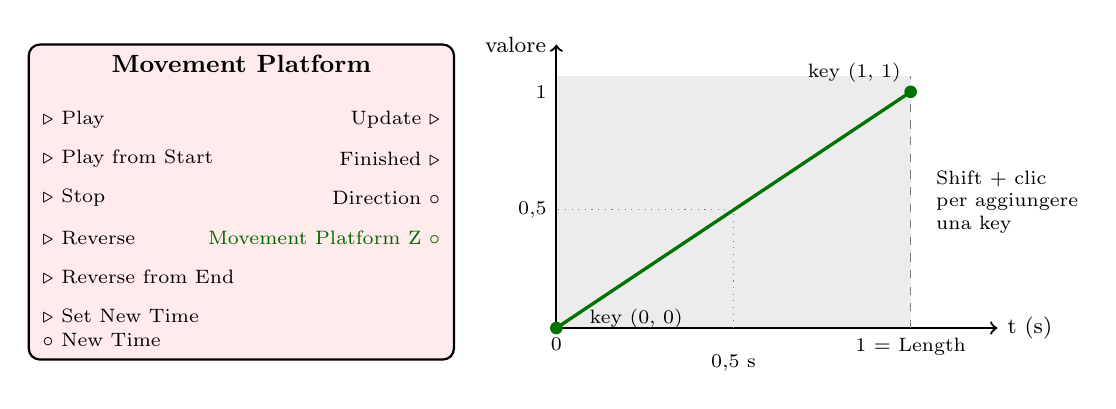
\begin{tikzpicture}[font=\footnotesize,
  ue6tl/.style={draw, thick, rounded corners=4pt, fill=red!8, minimum width=5.4cm,
                minimum height=4.0cm},
  ue6pin/.style={font=\scriptsize}]
  % nodo
  \node[ue6tl] (tl) at (0,0) {};
  \node[font=\small\bfseries] at (0,1.75) {Movement Platform};
  \foreach \t [count=\k] in {Play, Play from Start, Stop, Reverse, Reverse from End,
                             Set New Time} {
    \node[ue6pin, anchor=west] at (-2.65,1.55-0.5*\k) {$\triangleright$ \t};
  }
  \node[ue6pin, anchor=west] at (-2.65,-1.75) {$\circ$ New Time};
  \node[ue6pin, anchor=east] at (2.65,1.05) {Update $\triangleright$};
  \node[ue6pin, anchor=east] at (2.65,0.55) {Finished $\triangleright$};
  \node[ue6pin, anchor=east] at (2.65,0.05) {Direction $\circ$};
  \node[ue6pin, anchor=east, text=green!40!black] at (2.65,-0.45) {Movement Platform Z
    $\circ$};
  % curva
  \begin{scope}[xshift=4.0cm, yshift=-1.6cm]
    \fill[gray!15] (0,0) rectangle (4.5,3.2);
    \draw[->, thick] (0,0) -- (5.6,0) node[right]{t (s)};
    \draw[->, thick] (0,0) -- (0,3.6) node[left]{valore};
    \draw[gray, dashed] (4.5,0) -- (4.5,3.2);
    \node[font=\scriptsize, below] at (4.5,0) {1 = Length};
    \node[font=\scriptsize, below] at (0,0) {0};
    \node[font=\scriptsize, left] at (0,3.0) {1};
    \node[font=\scriptsize, left] at (0,1.5) {0,5};
    \draw[very thick, green!45!black] (0,0) -- (4.5,3.0);
    \fill[green!45!black] (0,0) circle (0.08);
    \fill[green!45!black] (4.5,3.0) circle (0.08);
    \node[font=\scriptsize, right] at (0.3,0.12) {key (0, 0)};
    \node[font=\scriptsize, above left] at (4.5,3.0) {key (1, 1)};
    \draw[gray, dotted] (2.25,0) -- (2.25,1.5) -- (0,1.5);
    \node[font=\scriptsize, align=center] at (2.25,-0.45) {0,5 s};
    \node[font=\scriptsize, align=left, anchor=west] at (4.7,1.6) {Shift + clic\\per
      aggiungere\\una key};
  \end{scope}
\end{tikzpicture}
\caption{Il nodo Timeline della piattaforma e la sua float track. A sinistra i sei
ingressi di esecuzione e le uscite: Update, Finished, Direction e il pin della traccia.
A destra la curva: Length 1 secondo (la zona grigia), due key in (0, 0) e (1, 1); a metà
del tempo il valore è a metà. Schema ricostruito.}
\label{ue6:fig:timeline}
\end{figure}

\begin{table}[htbp]
\centering
\small
\begin{tabular}{@{}p{3.4cm}p{10.6cm}@{}}
\toprule
\textbf{Pin} & \textbf{Che cosa fa} \\
\midrule
Play & riprende dal tempo attuale, in avanti \\
Play from Start & torna a 0 e va in avanti \\
Stop & ferma la timeline dove si trova \\
Reverse & riprende dal tempo attuale, all'indietro \\
Reverse from End & salta alla fine e va all'indietro \\
Set New Time & porta la timeline al tempo New Time \\
\midrule
Update & scatta a ogni aggiornamento mentre la timeline scorre \\
Finished & scatta quando la timeline arriva a un estremo (la fine in avanti, l'inizio
all'indietro) \\
Direction & la direzione attuale: Forward o Backward (un'enumerazione,
\emph{ETimelineDirection}) \\
una uscita per traccia & il valore della traccia al tempo attuale (float, vettore,
colore); le Event track hanno invece un'uscita di esecuzione \\
\bottomrule
\end{tabular}
\caption{I pin del nodo Timeline.}
\label{ue6:tab:timeline}
\end{table}

\paragraph{Approfondimento: le timeline secondo Romero e Sewell.} Nel capitolo 6
(\emph{Enhancing Player Abilities}) i due autori usano una timeline per lo
\emph{zoom} del mirino: una float track \emph{Field of View} da 90 a 45 in 0,3 secondi,
collegata dall'Update al nodo \emph{Set Field of View}, con il tasto premuto su Play e il
tasto rilasciato su \textbf{Reverse}, esattamente lo schema che la lezione userà per la
piattaforma che sale e scende. Il libro aggiunge due osservazioni. La prima: le timeline
sono perfette ``per semplici cambi di valore, come la rotazione di una porta''; per
animazioni complesse, di personaggi o cinematiche, Unreal ha il \textbf{Sequencer}. La
seconda (nella tabella che confronta macro, funzioni ed eventi): i nodi Timeline si
possono usare solo nell'\textbf{Event Graph} di un actor, non dentro le funzioni né
dentro le macro, perché, come i Delay, sono azioni che durano nel tempo. Nelle opzioni
in cima all'editor ci sono poi \textbf{Auto Play} (parte da sola al Begin Play),
\textbf{Loop} (ricomincia all'infinito, utile per un'altalena) e \textbf{Use Last
Keyframe} (fa finire la timeline sull'ultima key invece che alla Length). Le key, con il
tasto destro, possono avere interpolazione lineare, costante o \emph{auto} (curva
morbida, con le tangenti): una curva a ``S'' fa partire e arrivare la piattaforma
dolcemente, invece che di colpo.

% ---------------------------------------------------------------------
\section{L'interpolazione lineare e l'alfa}
\label{ue6:sec:lerp}

``Adesso ci servirebbe fare quello che viene chiamato, in informatica e anche su Unreal,
\textbf{interpolazione}.'' C'è una slide: l'\textbf{interpolazione lineare} ``ci dice:
passo da questo punto a questo punto, passandomi per tutti gli intermedi'', con un
\textbf{alfa}.

\paragraph{L'esempio delle animazioni.} ``L'interpolazione è un concetto che possiamo
trovare in tante cose diverse, tra cui le animazioni.'' Per muovere gli arti di un
personaggio si usano le \textbf{ossa}, interne alla \emph{mesh}. Il docente muove il
braccio davanti alla webcam: ``io non è che vedo subito così, pa!, di scatto: passo
proprio da questo a questo''. ``L'interpolazione è il passaggio per tutti i punti
intermedi che mi fa arrivare alla posizione finale.''

\paragraph{L'alfa.} ``Seguitemi bene attentamente, ragazzi.'' Su una linea che va da 0 a
100, l'alfa è ``un \textbf{puntatore} del punto in cui ci troviamo'', espresso da 0 a 1.
Se siamo a 0, l'alfa è 0; se siamo a 100, l'alfa è 1; ``se l'alfa sta a 0,5, ci
troveremo alla sua metà''. Domanda: se siamo a 20? Uno studente: ``0,2''. ``Ottimo. Siamo
a 0,2: l'alfa sarà a 0,2.'' ``Ci sono varie tipologie di interpolazione, ma
l'interpolazione funziona in questo modo'' (figura~\ref{ue6:fig:lerp}).

\begin{figure}[htbp]
\centering
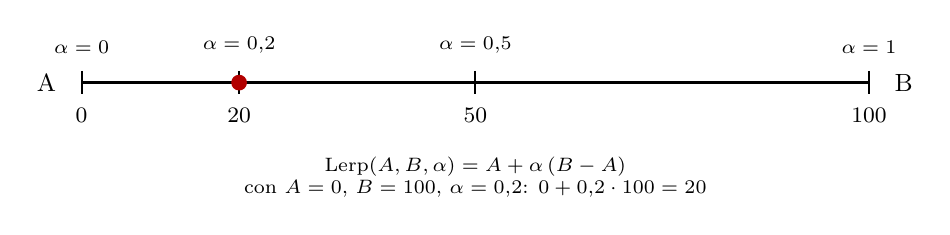
\begin{tikzpicture}[font=\footnotesize]
  \draw[very thick] (0,0) -- (10,0);
  \foreach \x/\l in {0/0, 2/20, 5/50, 10/100} {
    \draw[thick] (\x,0.15) -- (\x,-0.15);
    \node[below] at (\x,-0.2) {\l};
  }
  \node[above, font=\scriptsize] at (0,0.25) {$\alpha = 0$};
  \node[above, font=\scriptsize] at (2,0.25) {$\alpha = 0{,}2$};
  \node[above, font=\scriptsize] at (5,0.25) {$\alpha = 0{,}5$};
  \node[above, font=\scriptsize] at (10,0.25) {$\alpha = 1$};
  \node[left, font=\small] at (-0.2,0) {A};
  \node[right, font=\small] at (10.2,0) {B};
  \fill[red!70!black] (2,0) circle (0.1);
  \node[align=center, font=\scriptsize] at (5,-1.2) {$\mathrm{Lerp}(A, B, \alpha) = A +
    \alpha\,(B - A)$\\con $A = 0$, $B = 100$, $\alpha = 0{,}2$: $0 + 0{,}2 \cdot 100 =
    20$};
\end{tikzpicture}
\caption{L'alfa dell'interpolazione lineare: un numero da 0 a 1 che dice in che punto
del segmento da A a B ci troviamo. L'esempio della lezione: a 20 su 100 l'alfa vale
0,2. La formula, sotto, non è stata scritta a lezione ma è quella che il nodo Lerp
calcola. Schema ricostruito.}
\label{ue6:fig:lerp}
\end{figure}

\paragraph{Approfondimento: Lerp, alfa e timeline.} Il nodo \textbf{Lerp} (per i float)
calcola $A + \alpha(B - A)$: con $\alpha = 0$ restituisce A, con $\alpha = 1$
restituisce B, e in mezzo i valori intermedi in proporzione. Esiste per i vettori
(\textbf{Lerp (Vector)}, che interpola X, Y e Z con lo stesso alfa), per le rotazioni
(\textbf{Lerp (Rotator)}, con l'opzione \emph{Shortest Path}), per i colori e per i
\emph{transform}. L'alfa può anche uscire da $[0, 1]$: con 1,2 il risultato va oltre B
(estrapolazione). Il binomio timeline--Lerp è classico perché divide i compiti: la
\textbf{timeline} decide \emph{come} si scorre nel tempo (quanto dura, con che curva,
avanti o indietro), il \textbf{Lerp} decide \emph{dove} si va (da A a B). Cambiare la
durata o la forma del movimento non tocca A e B, e viceversa. Da non confondere con i nodi
\emph{FInterp To} e \emph{RInterp To} (quest'ultimo usato per la torretta): quelli
avvicinano ogni frame un valore al bersaglio di una frazione, con una velocità e il
Delta Time, senza un alfa né una durata fissa.

% ---------------------------------------------------------------------
\section{Il primo metodo: un Lerp sulla Z}
\label{ue6:sec:metodo1}

``Abbiamo quindi da tirare fuori il nostro bellissimo \textbf{Lerp}.'' Domanda di
partenza, guardando la piattaforma: ``quale asse dovremmo influenzare, che si muova nel
tempo?'' ``La Z.'' ``Ottimo, bravo, Federico.''

\paragraph{La costruzione.} Il docente procede per tentativi, e a un certo punto uno
studente chiede: ``potresti spiegare un po' tutti i passaggi? Perché a un certo punto mi
sono perso''. La versione rispiegata, che è quella da seguire, è questa
(figura~\ref{ue6:fig:metodo1}).
\begin{enumerate}
  \item Si prende il componente \textbf{Platform} e si tira fuori \textbf{Get Relative
        Location}. All'inizio il docente aveva usato Get Actor Location, poi la World
        Location (``scusate, ragazzi, questa è world''), e infine la \emph{relative},
        cioè la posizione rispetto all'actor. Si splitta il vettore.
  \item La \textbf{Z} relativa va, da sola, nel pin \textbf{A} del Lerp: il punto di
        partenza.
  \item La stessa Z più una variabile float nuova, \textbf{MaxHeight}, va nel pin
        \textbf{B}: il punto d'arrivo. Il valore scelto è \textbf{70} (``ci piace 70'';
        ``sono 70 unità sulla Z'').
  \item L'\textbf{Alpha} del Lerp è il pin \textbf{Movement Platform Z} della timeline.
  \item Un \textbf{Make Vector}: X e Y dalla location relativa, invariate; Z dal Lerp.
  \item \textbf{Set Relative Location} sul componente Platform, con il Make Vector nel
        pin \emph{New Location}, eseguito dall'\textbf{Update} della timeline.
\end{enumerate}
La timeline parte dal Begin Overlap della box, attraverso il Branch sul player, con
\textbf{Play}.

\begin{figure}[htbp]
\centering
\begin{tikzpicture}[font=\footnotesize,
  ue6node/.style={draw, thick, rounded corners=4pt, align=center, fill=gray!8,
                  minimum height=0.8cm, text width=2.1cm},
  ue6event/.style={ue6node, fill=red!12},
  ue6exec/.style={-{Stealth[length=2.5mm]}, very thick, black!80},
  ue6data/.style={-{Stealth[length=2mm]}, thick, green!45!black},
  ue6vec/.style={-{Stealth[length=2mm]}, thick, yellow!50!black}]
  \node[ue6event, text width=2.5cm] (ov) at (0,0) {\textbf{On Component Begin
    Overlap} (Box)};
  \node[ue6node, text width=2.4cm] (eq) at (0,-1.8) {Other Actor \textbf{==}\\\textbf{Get
    Player Pawn}};
  \node[ue6node, text width=1.3cm] (br) at (3.0,0) {\textbf{Branch}};
  \node[ue6node, text width=2.3cm] (tl) at (5.8,0) {\textbf{Timeline}\\Movement
    Platform};
  \node[ue6node, text width=2.4cm] (set) at (11.0,0) {\textbf{Set Relative
    Location}\\(Platform)};
  \node[ue6node, text width=2.5cm] (grl) at (3.0,-3.6) {Platform $\rightarrow$
    \textbf{Get Relative Location} (split)};
  \node[ue6node, text width=1.8cm] (mh) at (5.8,-3.6) {Z +\\\textbf{MaxHeight} (70)};
  \node[ue6node, text width=1.4cm] (lerp) at (8.2,-2.0) {\textbf{Lerp}\\A, B, Alpha};
  \node[ue6node, text width=1.7cm] (mv) at (11.0,-2.0) {\textbf{Make Vector}};
  \draw[ue6exec] (ov) -- (br);
  \draw[ue6exec] (br) -- node[above, font=\scriptsize]{True} node[below,
    font=\scriptsize]{Play} (tl);
  \draw[ue6exec] (tl) -- node[above, font=\scriptsize]{Update} (set);
  \draw[-{Stealth[length=2mm]}, thick, red!60!black] (eq.north) -- node[right,
    font=\scriptsize]{bool} (br.south west);
  \draw[ue6data] (tl.south) -- node[left, font=\scriptsize, pos=0.3]{Z track} (lerp.west);
  \draw[ue6data] (grl.north) |- node[pos=0.25, left, font=\scriptsize]{Z $\rightarrow$ A}
    ([yshift=-0.2cm]lerp.west);
  \draw[ue6data] (grl) -- (mh);
  \draw[ue6data] (mh.east) -| node[pos=0.7, right, font=\scriptsize]{B} (lerp.south);
  \draw[ue6data] (lerp) -- node[above, font=\scriptsize]{Z} (mv);
  \draw[ue6data] (grl.south) -- ++(0,-0.35) -| node[pos=0.25, below,
    font=\scriptsize]{X, Y} (mv.south);
  \draw[ue6vec] (mv) -- node[right, font=\scriptsize]{New Location} (set);
\end{tikzpicture}
\caption{Il primo metodo. Il Begin Overlap della box, se l'actor è il player, fa
partire la timeline; a ogni Update un Lerp tra la Z relativa attuale (A) e la stessa Z
più MaxHeight (B), con la traccia della timeline come alfa, diventa la nuova Z della
Platform. Funziona, ma ha un difetto: A e B vengono riletti a ogni Update dalla posizione
già spostata (vedi l'approfondimento). Schema ricostruito.}
\label{ue6:fig:metodo1}
\end{figure}

\paragraph{``Va altissimo''.} In Play la piattaforma sale, ma molto più di 70 unità: a uno
studente, con 70, ``arriva in cielo''; con 30 arriva ``poco più alto del muretto'' della
scena. ``Non so perché, però sia così diverso.'' Il docente promette un metodo ``un po'
più carino e più malleabile''; la spiegazione arriva, in parte, dopo la pausa: ``stiamo
sommando'' (sezione~\ref{ue6:sec:playrate}).

\paragraph{Approfondimento: perché il primo metodo ``somma''.} A ogni Update il grafo
legge la Z \emph{attuale} della Platform, che è già stata spostata dall'Update
precedente, e la usa come A; B è quella Z più 70. Il risultato è quindi
$Z_{\text{nuova}} = Z_{\text{attuale}} + \alpha \cdot 70$: non un punto tra due estremi
fissi, ma un \emph{incremento} che si accumula. Se la timeline si aggiorna $N$ volte in
un secondo, la piattaforma sale di circa $70 \cdot \sum \alpha_k \approx 70 \cdot N/2$
unità: con 60 aggiornamenti al secondo, più di duemila, non settanta. Da qui tre
conseguenze, tutte osservate a lezione. La salita dipende dal \emph{frame rate} (``è la
mia impressione che vada più in alto'': su un computer più veloce, più somme). Rallentare
la timeline con il play rate fa \emph{più} somme, e la piattaforma sale ancora di più;
accelerarla ne fa meno. E con il Reverse il calcolo non torna simmetrico: lo studente
che si vedeva la piattaforma ``sempre leggermente più in basso fino a scomparire sotto il
terreno'' stava osservando proprio l'errore che si accumula a ogni salita e discesa. La
cura è leggere A e B \emph{una volta sola}, prima che la timeline parta, e tenerli fissi:
è il secondo metodo.

% ---------------------------------------------------------------------
\section{La pausa e il Nintendo Direct}
\label{ue6:sec:pausa}

``Sono le 17:37. Facciamo la pausa classica di 20 minuti''; si torna ``alle 18''. Durante
la pausa il docente aiuta uno studente con la foto del codice mandata su Discord (il
problema è l'altezza della piattaforma con il primo metodo: ``70 è giusto'', il resto
``credo sia tutto giusto''), e poco prima della ripresa arrivano le notizie dal
\emph{Nintendo Direct}, riferite da uno studente ``referente''. Nella trascrizione,
molto storpiata, si riconoscono un \emph{remake} di \emph{Ocarina of Time} (``l'Opera of
Time Remake''), un nuovo \emph{Xenoblade}, un \emph{Final Fantasy} in 2D-HD ``stile
\emph{Octopath Traveler}'' e del materiale nuovo su \emph{Deltarune}; il tutto è riportato
come lo si legge nella trascrizione, senza verifiche. La chiacchierata scivola su
\emph{Kingdom Hearts} e sulla trilogia \emph{remake} di \emph{Final Fantasy VII} (``uscirà
prima l'intera trilogia remake''), e su Tetsuya Nomura (``le nomurate''). ``Comunque,
sempre belli questi siparietti'', dice il docente; chi segue in differita può
partecipare alla conversazione su Discord, ``pacificamente''.

% ---------------------------------------------------------------------
\section{La velocità della timeline: Set Play Rate e Duration}
\label{ue6:sec:playrate}

``Allora riprendiamo la nostra bellissima \emph{elevator}, o piattaforma, quello che
vogliamo.'' Una cosa che si può controllare è il \textbf{play rate}: ``la velocità in cui
essa, sempre ripetendo un secondo, viene detta: vai a due volte la tua velocità, a metà
della tua velocità''.

\paragraph{La timeline è un componente.} ``Se avete notato'', nel pannello
\textbf{Components} del Blueprint, accanto a Box, Platform e DefaultSceneRoot, c'è anche
\textbf{Movement Platform}: ``lo stesso nome della timeline''. Ogni timeline aggiunta
crea un componente con il suo nome, e da quel componente si possono chiamare le sue
funzioni. Trascinandolo nel grafo (``Ctrl per il Get''), se ne tira fuori \textbf{Set
Play Rate}, con il \emph{Target} sulla timeline.

\paragraph{Play rate e lunghezza.} Sul \textbf{Begin Play}, Set Play Rate a 0,5: ``la
sua velocità sarà la metà''; a 2, ``il doppio''; a 1, ``andrà come prima''. Il docente
insiste: ``il play rate \textbf{non è la lunghezza}, non è la Length, è diversa''. La
Length dice quanto è lunga la curva; il play rate dice quanto velocemente la si
percorre.

\paragraph{Il primo metodo non regge.} Con il play rate cambiato, la piattaforma del primo
metodo si comporta in modo strano, e il docente ne dà la spiegazione: ``stiamo
aumentando di 30 a ogni frame del nostro secondo''; ``se riduciamo il play rate, lui
sarà più veloce, ma di conseguenza farà meno somme''. Detto meglio: con un play rate più
alto la timeline finisce prima, fa meno Update, e quindi meno somme; con uno più basso ne
fa di più. ``Vedete che non si ferma a quell'unità, perché in questo caso stiamo sommando
solamente: se finisce prima, vuol dire che finirà prima.''

\paragraph{La variabile Duration.} Ragionare in velocità relative è scomodo; è più
naturale dire ``voglio che duri 2 secondi''. Una variabile float \textbf{Duration} e un
piccolo calcolo:
\[
  \text{Play Rate} = \frac{1}{\text{Duration}} \times \text{Timeline Length},
\]
con \textbf{Divide} (``lo slash'') e \textbf{Get Timeline Length} (dal componente della
timeline) moltiplicati con \textbf{Multiply}, e il risultato nel Set Play Rate del Begin
Play. Con Duration 1 e una Length di 1 il play rate è 1, ``velocità normale''. Con
Duration 2 il docente prima dice ``il doppio'', poi si corregge: ``no, scusa, sarà più
lunga, perdonate''; con 0,5 sarà più veloce. È ``una variabile d'appoggio'' che traduce
una durata in secondi nel play rate giusto. Per il resto della lezione la Duration resta
a 1, ``così almeno siamo tranquilli''.

\paragraph{Approfondimento: perché la formula funziona.} Una timeline di lunghezza $L$
percorsa con play rate $r$ dura $L / r$ secondi. Volendo che duri $D$ secondi, basta
porre $L / r = D$, cioè $r = L / D$: è la formula del docente, scritta come $1/D \times
L$. Moltiplicare per la Length rende il calcolo indipendente dalla curva: se un giorno la
timeline diventa lunga 3 secondi, la Duration continua a dire la durata vera. Due
cautele. Una Duration a 0 produce una divisione per zero, e la timeline non si muove più
(il primo sospetto, a lezione, quando la piattaforma di uno studente ``ha smesso di
muoversi''). E il Set Play Rate va chiamato sulla timeline \emph{giusta}: è l'errore
della sezione~\ref{ue6:sec:timelinesbagliata}.

% ---------------------------------------------------------------------
\section{Il secondo metodo: il Billboard e le posizioni salvate}
\label{ue6:sec:metodo2}

Per avere ``due punti specifici da raggiungere, in modo non dipendente da dei valori'',
il docente rifà il grafo. Il vecchio si può tenere, staccato, e copiare (``Ctrl+C,
Ctrl+V'') i pezzi che servono; il Set Relative Location della Platform resta: ``non lo
cancellate, perché è giusto che sia così''.

\paragraph{Il Billboard.} Si aggiunge (\emph{Add}) un componente \textbf{Billboard}:
``un oggetto di questo tipo: è questo \textbf{dinosauro}''. ``Fondamentalmente è un punto
nello spazio'', come lo \emph{Scene Component} già usato per la torretta; ``la
differenza è che ha un'immagine'', visibile solo nell'editor. Il piano: ``prendere la sua
posizione nello spazio, e dire: \emph{lerpami} da questa posizione della piattaforma
iniziale a questa posizione del billboard''. Il Billboard si mette a \textbf{500} sulla
Z (``o di più? 700? Mettete 500, la metà è giusta'').

\paragraph{Lerp (Vector).} Al posto del Lerp sui float, un \textbf{Lerp (Vector)} (``un
v-lerp, un lerp tra vettori''): ``invece che tra due numeri, due float, tra due
vettori''. A è la \textbf{Get Relative Location} della Platform, B quella del Billboard,
l'Alpha la traccia della timeline; l'uscita va direttamente nel Set Relative Location
della Platform, senza Make Vector.

\paragraph{``C'è qualcosa di sbagliato?''} Così com'è, avverte il docente, il grafo ha
ancora il difetto del primo metodo: ``non salviamo mai la posizione delle due''. Se il
Billboard fosse \textbf{attaccato} alla Platform, ``si muoverà insieme ad essa'', e
allora ``avremo un effetto infinito'': la piattaforma insegue un bersaglio che si
allontana, ``un continuo movimento sempre in alto, sempre in alto, pom pom pom''. Il
docente lo mostra riattaccando il Billboard: ``e si ricomincia''. La cura:
\begin{enumerate}
  \item i due Get Relative Location si spostano sul \textbf{Begin Play};
  \item sul pin di uscita di ciascuno, \textbf{Promote to Variable}: la Platform diventa
        \textbf{StartLocation}, il Billboard \textbf{FinishLocation};
  \item nel Lerp (Vector) entrano i \emph{Get} delle due variabili: StartLocation in A,
        FinishLocation in B.
\end{enumerate}
``Così facendo abbiamo delle variabili che sono sempre fisse'': ``sarà sempre la stessa
posizione'' (figura~\ref{ue6:fig:metodo2}).

\paragraph{Il bello del Billboard.} ``La cosa bella, poi, che possiamo vedere con questo
metodo'': il dinosauro si può spostare nello spazio, nei dettagli della piattaforma, e la
piattaforma raggiungerà quel punto. ``Dovete fare un livello? L'avete alzato a 8 metri?
Prendete il billboard, lo mettete a 800'': ``devo arrivare qua sopra, quindi arriverò
qua. Ecco fatto, sono arrivato preciso''. (``Salto, l'ho mancato malissimo.'') E non solo
in verticale: spostando il Billboard anche sulla X o sulla Y, ``andrà in diagonale'';
``potremmo pure fare piattaforme in orizzontale, in diagonale, come vi pare''. ``Invece
di fare matematica'', si prendono direttamente i due vettori.

\paragraph{Il ritorno: Reverse.} Scendendo dalla piattaforma, questa ``rimane là''.
``Vi potrei dire: facciamo una nuova timeline e la facciamo al contrario. Non serve.
Perché abbiamo \textbf{Reverse}.'' L'\textbf{On Component End Overlap} della box,
collegato al pin Reverse della timeline: ``esco fuori e lei se ne torna al suo posto'',
perché ``invece di fare da A a B, fa da B ad A. Questo è insito nella timeline''.

\begin{figure}[htbp]
\centering
\begin{tikzpicture}[font=\footnotesize,
  ue6node/.style={draw, thick, rounded corners=4pt, align=center, fill=gray!8,
                  minimum height=0.8cm, text width=2.1cm},
  ue6event/.style={ue6node, fill=red!12},
  ue6var/.style={ue6node, fill=blue!10, rounded corners=8pt},
  ue6exec/.style={-{Stealth[length=2.5mm]}, very thick, black!80},
  ue6data/.style={-{Stealth[length=2mm]}, thick, green!45!black},
  ue6vec/.style={-{Stealth[length=2mm]}, thick, yellow!50!black}]
  % Begin Play
  \node[ue6event, text width=2.4cm] (bp) at (0,0) {\textbf{Event Begin Play}};
  \node[ue6node, text width=2.3cm] (s1) at (3.3,0) {\textbf{Set}\\StartLocation};
  \node[ue6node, text width=2.3cm] (s2) at (6.4,0) {\textbf{Set}\\FinishLocation};
  \node[ue6node, text width=2.2cm] (pr) at (9.6,0) {\textbf{Set Play Rate}\\($1/D \times
    L$)};
  \node[ue6node, text width=2.5cm] (g1) at (3.3,-1.6) {Platform $\rightarrow$ Get
    Relative Location};
  \node[ue6node, text width=2.5cm] (g2) at (6.4,-1.6) {Billboard $\rightarrow$ Get
    Relative Location};
  \draw[ue6exec] (bp) -- (s1);
  \draw[ue6exec] (s1) -- (s2);
  \draw[ue6exec] (s2) -- (pr);
  \draw[ue6vec] (g1) -- (s1);
  \draw[ue6vec] (g2) -- (s2);
  % overlap e timeline
  \begin{scope}[yshift=-3.6cm]
    \node[ue6event, text width=2.6cm] (bo) at (-0.2,0) {\textbf{Begin Overlap}
      (Box)\\+ Branch sul player};
    \node[ue6event, text width=2.6cm] (eo) at (-0.2,-1.5) {\textbf{End Overlap} (Box)};
    \node[ue6node, text width=2.2cm, minimum height=2.2cm] (tl) at (3.6,-0.75)
      {\textbf{Timeline}\\Movement\\Platform};
    \node[ue6node, text width=1.9cm] (lv) at (7.0,-2.5) {\textbf{Lerp (Vector)}\\A, B,
      Alpha};
    \node[ue6var, text width=1.9cm] (v1) at (7.0,-4.0) {StartLocation};
    \node[ue6var, text width=2.1cm] (v2) at (9.8,-4.0) {FinishLocation};
    \node[ue6node, text width=2.4cm] (set) at (10.4,-0.4) {\textbf{Set Relative
      Location}\\(Platform)};
    \draw[ue6exec] (bo.east) -- node[above, font=\scriptsize]{Play} ([yshift=0.75cm]tl.west);
    \draw[ue6exec] (eo.east) -- node[below, font=\scriptsize]{Reverse}
      ([yshift=-0.75cm]tl.west);
    \draw[ue6exec] ([yshift=0.35cm]tl.east) -- node[above, font=\scriptsize]{Update}
      (set.west);
    \draw[ue6data] ([yshift=-0.6cm]tl.east) -| node[pos=0.25, above,
      font=\scriptsize]{Alpha} (lv.north);
    \draw[ue6vec] (v1) -- node[left, font=\scriptsize]{A} (lv);
    \draw[ue6vec] (v2.north) |- node[pos=0.25, right, font=\scriptsize]{B} (lv.east);
    \draw[ue6vec] (lv.east) -- ++(0.9,0) |- node[pos=0.2, right,
      font=\scriptsize]{New Location} (set.south west);
  \end{scope}
\end{tikzpicture}
\caption{Il secondo metodo. Sopra: al Begin Play le posizioni relative della Platform e
del Billboard vengono salvate una volta per tutte in StartLocation e FinishLocation (con
Promote to Variable), e si imposta il play rate dalla Duration. Sotto: il Begin Overlap
fa Play, l'End Overlap fa Reverse; a ogni Update un Lerp (Vector) tra i due punti fissi,
con la traccia come alfa, diventa la nuova posizione della Platform. Schema
ricostruito.}
\label{ue6:fig:metodo2}
\end{figure}

\paragraph{I problemi.} ``Problemi su questo? Siete a posto?'' Tre casi.
\begin{itemize}
  \item \textbf{``A me non si muove.''} Il docente ripassa la lista: le due Get Relative
        Location, le due variabili, la timeline in Play, l'Update, il Lerp tra i
        vettori, l'Alpha collegato. Lo studente non aveva capito come creare le
        variabili: tasto destro sul pin, \textbf{Promote to Variable}, e il nome. Poi
        StartLocation in A, FinishLocation in B, e l'Alpha alla traccia della timeline.
  \item \textbf{L'evento diventato Custom Event.} Uno studente scopre da solo il suo
        errore: copiando e incollando il blocco, l'evento di overlap ``mi ha preso come
        Custom Event generico, e quindi non si muoveva''. Un evento di componente
        incollato in un Blueprint perde il legame con il componente e diventa un evento
        qualunque, che nessuno chiama. ``Errore di distrazione.''
  \item \textbf{Ero rimasto indietro.} Uno studente, che aveva ricevuto una telefonata,
        riceve il riassunto: Billboard, Get Relative Location della Platform in
        StartLocation e del Billboard in FinishLocation, il Lerp (Vector) con l'alfa, il
        Set Relative Location, e il Reverse sull'End Overlap.
\end{itemize}

\paragraph{Approfondimento: Billboard figlio di chi?} Il docente fa vedere che, con il
Billboard attaccato alla Platform, la piattaforma ``sale all'infinito'', e che salvando le
posizioni al Begin Play il problema scompare. Ma c'è un dettaglio che la lezione non
esplicita: se il Billboard resta figlio della Platform, la sua \emph{relative location}
è relativa alla Platform, non all'actor; salvarla al Begin Play dà $(0, 0, 500)$ rispetto
alla piattaforma, mentre il Set Relative Location della Platform lavora rispetto alla
radice dell'actor. I due numeri coincidono solo se la Platform sta nell'origine
dell'actor (come nel Blueprint della lezione). La configurazione più robusta è mettere il
Billboard come figlio della \textbf{DefaultSceneRoot}, accanto alla Platform, così che
le due posizioni relative siano nello stesso spazio e il bersaglio non si muova mai con
la piattaforma. Un'altra soluzione, equivalente, è salvare e impostare le posizioni nel
mondo (Get e Set World Location). Infine: il ``dinosauro'' è visibile solo nell'editor;
nel gioco il Billboard non si vede, come tutti i componenti di servizio.

% ---------------------------------------------------------------------
\section{La timeline sbagliata}
\label{ue6:sec:timelinesbagliata}

Il docente vuole far vedere che la Duration funziona anche con il secondo metodo: ``la
cambio in 2''; poi, ``mettiamo dei valori che posso riconoscere, tipo 10''. Ma la
velocità non cambia. ``Non mi setta il play rate, forse.'' Anche a uno studente,
``l'unica cosa è la duration: non va effettivamente a modificare la velocità''. Il
docente prova un Print, un play rate a 0,1, a mille: ``sempre lo stesso''.

\paragraph{La soluzione, da uno studente.} ``Domanda un po' stupida: non è che forse
l'attore deve essere Platform e non Movement Platform?'' Non è quello, ma è la pista
giusta: ``errore mio''. Il secondo metodo usa una timeline \emph{nuova}, che si chiama
semplicemente \textbf{Timeline}; il Set Play Rate del Begin Play aveva come Target ancora
\textbf{Movement Platform}, ``quella dell'esempio di prima''. ``Stavamo referenziando la
timeline dell'altro esempio, e non la playavamo mai.''

\paragraph{La lezione dell'errore.} ``Da questo errore possiamo imparare qualche cosa'':
``le timeline hanno un \textbf{nome}''. Ogni timeline è un componente distinto, e le sue
funzioni (Set Play Rate, Get Timeline Length, Play, Reverse\ldots) agiscono solo su di
lei. Con il Target giusto e una Duration di 3, la piattaforma ``adesso è più lenta,
perché dura di più''. Morale: dare alle timeline nomi chiari, e cancellare quelle che non
servono più.

% ---------------------------------------------------------------------
\section{L'audio: la Sound Cue}
\label{ue6:sec:cue}

``Se non ci sono più problemi, passiamo al nostro bellissimo \emph{sound}.''

\paragraph{Importare il file.} Un consiglio d'ordine: una \textbf{cartella audio} nel
Content Browser (tasto destro, \emph{New Folder}). Per importare il file scaricato da
Discord basta \textbf{trascinarlo} nel Content Browser: appare un asset ``con la linea'',
una \textbf{Sound Wave}, senza altre domande.

\paragraph{Creare la Cue.} Sulla Sound Wave, tasto destro, \textbf{Create Cue} (``è il
secondo''). La \textbf{Sound Cue} (``la queue'', ``la Q'', nella trascrizione) è, dice il
docente, ``un \emph{sound} programmabile, tra virgolette''. Doppio clic: si apre un grafo
``come abbiamo visto anche su Unreal molto spesso'', con un nodo \textbf{Wave Player}
(il nostro suono) collegato all'\textbf{Output}. A sinistra, i dettagli della Cue:
\textbf{Volume Multiplier}, \textbf{Pitch Multiplier}, \emph{Sound Class} (``class
override''), \emph{Attenuation} e così via, ``tutti i vari dati che possiamo
modificare''.

\paragraph{Il pitch.} Con il Pitch Multiplier a 2 il suono è più alto; a 0,5 ``è pitchato
verso il basso'': ``molto più basso livello di tono, e anche più lento''. ``Perché il
pitch influenza sia la velocità sia la tonalità.'' Si torna a 1.

\paragraph{Il loop.} Con Play il suono parte ``solo una volta''; ``noi vogliamo che vada
in loop'' finché la piattaforma si muove, ``tipo: pipi, pipi, pipi''. Sul nodo
\textbf{Wave Player} si spunta \textbf{Looping}. (``Ovviamente rompe'': con la barra
spaziatrice si avvia e si interrompe l'anteprima.)

\paragraph{Il Modulator.} ``Vogliamo che magari il pitch o il volume siano un valore
\textbf{randomico}, tra un valore e un altro, in modo che non sia sempre lo stesso
suono.'' Si inserisce un nodo \textbf{Modulator} tra il Wave Player e l'Output: ha
\textbf{Pitch Min}, \textbf{Pitch Max}, \textbf{Volume Min} e \textbf{Volume Max}. I
valori della lezione: pitch tra \textbf{1,7} e \textbf{2}, volume tra \textbf{1} e
\textbf{1,2}. A ogni riproduzione il suono è ``leggermente più basso, leggermente più
alto''. Il perché, con il gioco della palla del docente: quando rimbalza fa un
\emph{boing}, ``e visto che avevo solo un suono'', che ripetuto ``sembra la stessa
cosa'', un pitch minimo e massimo hanno dato ``un risultato molto più gradevole''.

\paragraph{Il Random.} ``Esiste anche il \textbf{Random}'': se si hanno più suoni, il
nodo Random ne sceglie uno a caso a ogni riproduzione. Il docente lo prova mettendo nel
Random due rami, uno con il Modulator e uno senza, e ascoltando quale esce. L'uso tipico:
``un proiettile che prende un muro: invece di avere sempre lo stesso suono, mettete tutti
e tre i suoni nel Random''. Per la piattaforma non serve, e si torna al solo Modulator
(figura~\ref{ue6:fig:cue}).

\begin{figure}[htbp]
\centering
\begin{tikzpicture}[font=\footnotesize,
  ue6snode/.style={draw, thick, rounded corners=4pt, align=center, fill=violet!10,
                   minimum height=1.0cm, text width=2.5cm},
  ue6out/.style={draw, thick, rounded corners=4pt, align=center, fill=gray!20,
                 minimum height=1.0cm, text width=1.6cm},
  ue6aud/.style={-{Stealth[length=2.5mm]}, very thick, violet!60!black}]
  \node[ue6snode] (wp) at (0,0) {\textbf{Wave Player}\\SFX Moving Platform\\Looping
    \checkmark};
  \node[ue6snode] (mod) at (4.0,0) {\textbf{Modulator}\\Pitch 1,7--2\\Volume 1--1,2};
  \node[ue6out] (out) at (7.6,0) {\textbf{Output}};
  \draw[ue6aud] (wp) -- (mod);
  \draw[ue6aud] (mod) -- (out);
  \node[draw, dashed, rounded corners=4pt, align=left, text width=4.6cm, font=\scriptsize]
    at (11.4,0) {dettagli della Cue: Volume Multiplier, Pitch Multiplier (1), Sound
    Class, Attenuation\ldots};
  % variante random
  \begin{scope}[yshift=-2.4cm]
    \node[ue6snode, text width=2.0cm] (w1) at (0,0.6) {Wave Player 1};
    \node[ue6snode, text width=2.0cm] (w2) at (0,-0.6) {Wave Player 2};
    \node[ue6snode, text width=1.6cm] (rnd) at (4.0,0) {\textbf{Random}};
    \node[ue6out] (out2) at (7.6,0) {\textbf{Output}};
    \draw[ue6aud] (w1.east) -- (rnd.west);
    \draw[ue6aud] (w2.east) -- (rnd.west);
    \draw[ue6aud] (rnd) -- (out2);
    \node[align=left, font=\scriptsize, text width=4.6cm] at (11.4,0) {variante: più
      suoni, uno scelto a caso a ogni riproduzione (l'esempio del proiettile contro il
      muro)};
  \end{scope}
\end{tikzpicture}
\caption{La Sound Cue della piattaforma: il Wave Player in loop, un Modulator che varia
a caso pitch e volume a ogni riproduzione, l'Output. Sotto, la variante con il nodo
Random mostrata a lezione e poi scartata. Schema ricostruito.}
\label{ue6:fig:cue}
\end{figure}

\paragraph{Approfondimento: Sound Wave, Sound Cue, MetaSound.} La \textbf{Sound Wave} è
il file audio importato, con poche proprietà proprie (fra cui un suo \emph{Looping}). La
\textbf{Sound Cue} è un piccolo grafo che combina una o più Wave con nodi di
elaborazione: Modulator, Random, \emph{Mixer}, \emph{Concatenator}, \emph{Delay},
\emph{Attenuation}\ldots; nei Blueprint si può passare indifferentemente una Wave o una
Cue a qualunque nodo che vuole un \emph{Sound}. In Unreal Engine 5 esistono anche i
\textbf{MetaSound}, un sistema più recente e più potente, che genera e manipola l'audio
con un grafo simile a quello dei Blueprint; le Sound Cue restano supportate e sono il
punto di partenza più semplice. Il formato \textbf{WAV} raccomandato dal docente è quello
standard per l'import: non compresso, lo comprime poi l'engine secondo la piattaforma.
Sul pitch, l'osservazione del docente è esatta: in una Sound Cue il Pitch Multiplier
cambia la velocità di riproduzione, quindi alza o abbassa il tono e accorcia o allunga il
suono insieme, come un disco suonato a giri sbagliati.

% ---------------------------------------------------------------------
\section{Far suonare la piattaforma: Spawn Sound, Do Once e Stop}
\label{ue6:sec:suono}

``Abbiamo due modi per piazzare i suoni'': i nodi \textbf{Play Sound 2D} e \textbf{Play
Sound at Location}, e i nodi \textbf{Spawn Sound 2D} e \textbf{Spawn Sound at Location}.
``La differenza sostanziale è che uno \emph{playa} il suono solamente; l'altro lo
\emph{spawna}, e quindi crea una \textbf{referenza}'', come lo Spawn Actor from Class
``che quando spawna ha un Return Value''.

\paragraph{La prova con Play Sound 2D.} ``Proviamo a mettere Play Sound 2D'': la Cue
nel pin Sound, l'esecuzione dall'Update della timeline. Il docente sale sulla piattaforma: il suono parte,
``e non smette più''. Peggio: l'Update scatta a ogni aggiornamento, quindi i suoni si
sovrappongono (``come avete sentito, è stato uno stormo di uccelli incredibile''). Due
problemi, due soluzioni.
\begin{itemize}
  \item Il suono è in loop: per fermarlo bisogna sapere \emph{quale} suono fermare, e il
        Play Sound non lo dice. Serve lo \textbf{Spawn Sound at Location}, che
        restituisce la referenza.
  \item L'Update scatta molte volte: serve un \textbf{Do Once}, ``che lo fa una sola
        volta''.
\end{itemize}

\paragraph{Lo spawn.} \textbf{Do Once}, poi \textbf{Spawn Sound at Location}: Sound la
Cue, Location la \textbf{Get Actor Location} (``alla locazione dell'attore playerà questo
suono''; il docente pensa prima alla piattaforma, poi sceglie l'actor). Dal \textbf{Return
Value}, \textbf{Promote to Variable}: \textbf{SoundPlatform}. ``Adesso, di questo suono
che abbiamo creato, abbiamo la referenza: qualcosa che punta e ci dice: ehi, questo è il
suono che fa pipipipi.''

\paragraph{Lo stop.} ``Io voglio che si fermi quando la timeline finisce'', cioè quando
arriva in cima (a 1) o torna alla base (a 0). Sul \textbf{Finished} della timeline: Get
di SoundPlatform, \textbf{Stop}. ``Fino a che non è arrivato in cima, o fino a che non è
tornato alla base, il suono playerà, e si stopperà appena finisce la timeline.''

\paragraph{Il Reset del Do Once.} ``Un'ultima cosa molto importante.'' Il Do Once, una
volta passato, resta chiuso; ha però un ingresso \textbf{Reset}: ``se lo inserisco là
dentro, questo Do Once si resetta, si apre, e dà la possibilità di essere rieseguito''.
``Quando ho stoppato il suono una volta, lo devo riattivare per la volta dopo'': dopo lo
Stop, il Reset. ``E si ferma; scendo, ed eccolo. Benissimo.''

% ---------------------------------------------------------------------
\section{Il pitch che cambia con la direzione}
\label{ue6:sec:pitch}

``Potremmo anche, ipoteticamente\ldots'' L'idea: un suono \textbf{più alto quando la
piattaforma sale} e \textbf{più basso quando scende}. Il componente audio spawnato ha la
funzione \textbf{Set Pitch Multiplier}, da chiamare sulla referenza SoundPlatform.

\paragraph{Come sapere se sale o scende.} Il docente comincia a ragionare con un Branch
(``se sta andando da StartLocation a FinishLocation\ldots''), poi si ferma: ``possiamo
usare una cosa molto interessante''. Il pin \textbf{Direction} della timeline è
un'\textbf{enumerazione} (``che vedremo in seguito che cos'è, ma oggi ci serve
semplicemente vedere questa cosa''): ``una variabile che ha dentro di sé due elementi'',
\emph{Forward} e \emph{Backward}. Tirandone fuori uno \textbf{Switch on
ETimelineDirection} si ottengono due uscite di esecuzione: ``avanti vuol dire che sta
andando 0--1, e indietro è 1--0''.
\begin{itemize}
  \item \textbf{Forward}: Set Pitch Multiplier su SoundPlatform a \textbf{1}, il pitch
        normale;
  \item \textbf{Backward}: Set Pitch Multiplier a \textbf{0,4}, ``per far puh, puh, puh,
        un po' più bassino: una discesa'' (il docente prova anche 0,5 e 0,1, ``molto
        basso''; il valore finale è 0,4).
\end{itemize}
``Mettiamo tutto nel Do Once'' (figura~\ref{ue6:fig:suono}).

\paragraph{L'errore dell'ordine.} A una studentessa il grafo, ``sulla carta'', è giusto,
ma il compilatore segnala un errore: il Set Pitch Multiplier dice che il suono ``non è
mai stato creato''. Il motivo è l'ordine: lo Switch, con i due Set Pitch Multiplier,
veniva eseguito \emph{prima} che lo Spawn Sound avesse riempito la variabile, quindi su
una referenza vuota. ``Metti prima il Do Once'', e dopo lo spawn e il Set della
variabile, lo Switch con i due rami. ``Dovrebbe andare.'' E va (dopo aver condiviso anche
l'audio del computer su Zoom, per farlo sentire).

\begin{figure}[htbp]
\centering
\begin{tikzpicture}[font=\footnotesize,
  ue6node/.style={draw, thick, rounded corners=4pt, align=center, fill=gray!8,
                  minimum height=0.8cm, text width=2.0cm},
  ue6var/.style={ue6node, fill=blue!10, rounded corners=8pt},
  ue6exec/.style={-{Stealth[length=2.5mm]}, very thick, black!80},
  ue6data/.style={-{Stealth[length=2mm]}, thick, violet!60!black}]
  \node[ue6node, text width=2.0cm, minimum height=2.0cm] (tl) at (0,0)
    {\textbf{Timeline}};
  \node[ue6node, text width=1.5cm] (do) at (3.4,0.6) {\textbf{Do Once}};
  \node[ue6node, text width=2.4cm] (sp) at (6.1,0.6) {\textbf{Spawn Sound at
    Location}\\Cue, Get Actor Location};
  \node[ue6var, text width=2.1cm] (sv) at (9.1,0.6) {\textbf{Set}\\SoundPlatform};
  \node[ue6node, text width=2.1cm] (sw) at (12.0,0.6) {\textbf{Switch on
    ETimelineDirection}};
  \node[ue6node, text width=2.4cm] (f) at (12.0,2.4) {\textbf{Set Pitch
    Multiplier}\\1 (sale)};
  \node[ue6node, text width=2.4cm] (b) at (12.0,-1.2) {\textbf{Set Pitch
    Multiplier}\\0,4 (scende)};
  \node[ue6node, text width=2.2cm] (st) at (3.4,-1.9) {SoundPlatform $\rightarrow$
    \textbf{Stop}};
  \draw[ue6exec] ([yshift=0.6cm]tl.east) -- node[above, font=\scriptsize]{Update} (do);
  \draw[ue6exec] (do) -- (sp);
  \draw[ue6exec] (sp) -- (sv);
  \draw[ue6exec] (sv) -- (sw);
  \draw[ue6exec] (sw.north) -- node[right, font=\scriptsize]{Forward} (f.south);
  \draw[ue6exec] (sw.south) -- node[right, font=\scriptsize]{Backward} (b.north);
  \draw[ue6exec] ([yshift=-0.6cm]tl.east) -- ++(0.4,0) |- node[pos=0.3, left,
    font=\scriptsize]{Finished} (st.west);
  \draw[ue6exec] (st.north) -- node[left, font=\scriptsize]{Reset} (do.south);
  \draw[ue6data] (tl.south) -- (0,-3.1) -- node[below, font=\scriptsize, pos=0.85]{Direction}
    (10.5,-3.1) |- ([yshift=-0.25cm]sw.west);
  \draw[ue6data] (sp.south) -- ++(0,-0.4) -| node[pos=0.25, below, font=\scriptsize]{Return
    Value} (sv.south);
\end{tikzpicture}
\caption{Il suono della piattaforma. Al primo Update il Do Once lascia passare: lo Spawn
Sound at Location crea il suono in loop, la sua referenza viene salvata in SoundPlatform,
e lo Switch sulla Direction della timeline sceglie il pitch (1 in salita, 0,4 in
discesa). Al Finished, il suono si ferma e il Do Once si riapre per la volta dopo.
Schema ricostruito; l'ordine è quello che risolve l'errore della studentessa (prima lo
spawn, poi il pitch).}
\label{ue6:fig:suono}
\end{figure}

\paragraph{Approfondimento: Play o Spawn, 2D o at Location.} Romero e Sewell (capitolo 6)
usano \textbf{Play Sound at Location} per l'esplosione del bersaglio colpito: un suono
breve, ``spara e dimentica'', che non serve più controllare, con la \emph{Hit Location}
dell'Event Hit come posizione. Per un suono in loop, che va fermato o modificato, serve
invece uno dei nodi \textbf{Spawn Sound}, che creano un \textbf{Audio Component} e ne
restituiscono la referenza: su di esso si chiamano Stop, Set Pitch Multiplier, Set Volume
Multiplier, \emph{Fade Out} e così via. I nodi \textbf{2D} suonano ``in cuffia'', senza
posizione né attenuazione con la distanza (adatti a musica e interfaccia); quelli
\textbf{at Location} suonano in un punto del mondo, e con un'\emph{attenuation} si
sentono di meno allontanandosi. Due osservazioni sulla scelta della lezione. La prima: la
Get Actor Location è la posizione della \emph{radice} dell'actor, che non si muove,
perché a salire è solo la Platform; il suono resta quindi alla base. Per un suono che
segue la piattaforma esiste \textbf{Spawn Sound Attached}, che lo attacca a un componente
(qui, la Platform). La seconda: invece di Do Once e Spawn a ogni salita, si può aggiungere
un \textbf{Audio Component} direttamente ai componenti del Blueprint, con \emph{Auto
Activate} spento, e chiamare \emph{Play} e \emph{Stop} su di esso; la referenza c'è già,
e l'errore dell'ordine non può capitare.

% ---------------------------------------------------------------------
\section{La chiusura}
\label{ue6:sec:chiusura}

``Ci siete voi altri, ragazzi? C'è qualche problema? Funziona tranquillamente?'' ``Adesso
andiamo a cena, siamo a fine lezione.'' L'ultimo invito: ``se ci sono problemi, diteli
ora o tacete per sempre; o almeno fino alla prossima lezione''. L'appuntamento è per
\textbf{giovedì}. ``Vi ringrazio per l'attenzione. Buonasera a tutti, ragazzi. Ciao,
ciao.''

\begin{table}[htbp]
\centering
\small
\begin{tabular}{@{}p{5.4cm}p{8.6cm}@{}}
\toprule
\textbf{Sintomo} & \textbf{Causa e rimedio} \\
\midrule
Pop-up ``project files are not associated'' a ogni avvio del launcher & associazione
dei file di progetto rotta dagli aggiornamenti: Fix Now; i progetti non corrono rischi \\
Il messaggio di overlap non compare & la risposta di uno dei due oggetti è Ignore, o
manca Generate Overlap Events; con Overlap da una parte e Block dall'altra il risultato
è un overlap \\
I cubi si spawnano all'infinito, impilati & il trace sul Tick vede i cubi appena nati:
mesh di BP\_Cube su Custom, Visibility su Ignore (e Always Spawn, Ignore Collisions) \\
Il cubo si può solo scalare & è stato trascinato sopra il DefaultSceneRoot,
sostituendolo: ricrearlo come figlio della radice \\
``Un muro basso'' invece della griglia & cubi troppo grandi per l'intervallo di 100:
rimpicciolire BP\_Cube (0.5, 0.2) \\
Le righe non compaiono & il secondo ciclo usa la X di Get Actor Location invece della X
del primo ciclo, o somma l'offset alla X invece che alla Y \\
Il ciclo calcola ma non esegue & Loop Body non collegato al trace, o il trace non
collegato allo spawn \\
Il trace della riga non si vede & manca l'End (Up Vector $\times\,-5000$ sommato allo
Start) \\
Lag con la matrice & spawn e trace a ogni frame: Set Actor Tick Enabled (falso) sul
Completed del For Loop \\
La box non segue la piattaforma & la Box Collision non è figlia della Platform \\
La piattaforma sale troppo (``arriva in cielo'') & primo metodo: A e B riletti dalla
posizione già spostata, la salita si accumula; usare posizioni salvate (secondo metodo) \\
La piattaforma scende ogni volta un po' di più & stesso errore che si accumula a ogni
Play e Reverse: secondo metodo \\
La piattaforma insegue il Billboard all'infinito & il bersaglio si muove con la
Platform: salvare Start e Finish Location al Begin Play (e il Billboard figlio della
radice) \\
La piattaforma resta su quando si scende & End Overlap non collegato a Reverse \\
La piattaforma non si muove dopo un copia-incolla & l'evento di overlap incollato è
diventato un Custom Event generico: ricrearlo dal componente Box \\
Duration e play rate non hanno effetto & Set Play Rate sulla timeline sbagliata (il
Target è la timeline del primo metodo); o Duration a 0 \\
Il suono non smette più & Play Sound non dà una referenza: Spawn Sound at Location,
Promote to Variable, Stop sul Finished \\
Tanti suoni sovrapposti (``uno stormo di uccelli'') & lo spawn sull'Update scatta a ogni
aggiornamento: Do Once, con Reset dopo lo Stop \\
Il suono parte solo la prima volta & manca il Reset del Do Once \\
Errore su Set Pitch Multiplier (``mai creato'') & il pitch viene impostato prima dello
spawn: prima Do Once, Spawn e Set, poi lo Switch \\
\bottomrule
\end{tabular}
\caption{I problemi incontrati durante la lezione, con la causa e il rimedio.}
\label{ue6:tab:errori}
\end{table}

\begin{table}[htbp]
\centering
\small
\begin{tabular}{@{}p{4.4cm}p{9.6cm}@{}}
\toprule
\textbf{Nodo, componente o impostazione} & \textbf{Che cosa fa} \\
\midrule
Collision Presets / Collision Enabled & configurazioni pronte delle collisioni; attiva o
disattiva query (trace e overlap) e fisica \\
Object Type / Object Responses & la categoria dell'oggetto; come risponde (Ignore,
Overlap, Block) a ciascuna categoria \\
New Object Channel (Project Settings) & crea una nuova categoria di oggetti \\
Event ActorBegin/EndOverlap & inizio e fine di un overlap di un actor \\
On Component Begin/End Overlap & inizio e fine di un overlap di un componente (Other
Actor, Other Comp) \\
For Loop (Completed) & ripete il Loop Body da First a Last Index; Completed scatta alla
fine \\
Sequence & esegue in ordine le sue uscite Then 0, Then 1, \ldots \\
Break Hit Result & scompone l'Out Hit di un trace (Blocking Hit, Location, Impact Point,
Normal, \ldots) \\
Split Struct Pin & separa un pin struttura (un \emph{transform}, un vettore) nei suoi
campi \\
Set Actor Tick Enabled & accende o spegne l'Event Tick di un actor \\
Box Collision & un volume invisibile per overlap e collisioni \\
Billboard & un punto nello spazio con un'icona, visibile solo nell'editor \\
== (Equal) & confronta due valori o referenze; restituisce un booleano \\
Get Player Pawn & la referenza al Pawn controllato dal giocatore \\
Actor Has Tag & vero se l'actor ha il tag indicato \\
Timeline & una linea del tempo con tracce (Float, Vector, Event, Color); Play, Reverse,
Update, Finished, Direction \\
Set Play Rate / Get Timeline Length & velocità di una timeline; la sua lunghezza \\
Lerp / Lerp (Vector) & interpolazione lineare tra A e B con un alfa da 0 a 1 \\
Get / Set Relative Location & posizione di un componente rispetto al suo genitore \\
Make Vector & costruisce un vettore da X, Y, Z \\
Promote to Variable & crea una variabile del tipo di un pin e la imposta \\
Sound Wave / Sound Cue & il file audio importato; il grafo che lo elabora (Wave Player,
Looping, Modulator, Random) \\
Play Sound 2D / at Location & suona un suono e basta, senza referenza \\
Spawn Sound 2D / at Location & crea un Audio Component e ne restituisce la referenza \\
Stop / Set Pitch Multiplier & ferma un Audio Component; ne cambia il pitch \\
Do Once (Reset) & lascia passare l'esecuzione una volta, finché non viene resettato \\
Switch on ETimelineDirection & due uscite: Forward e Backward \\
\bottomrule
\end{tabular}
\caption{I nodi, i componenti e le impostazioni della sesta lezione.}
\label{ue6:tab:nodi}
\end{table}

% ---------------------------------------------------------------------
\section*{Punti chiave del capitolo}
\addcontentsline{toc}{section}{Punti chiave del capitolo}

\begin{itemize}
  \item Le risposte di collisione sono tre: \textbf{Ignore} (nessuna collisione,
        nessun evento), \textbf{Overlap} (gli oggetti si attraversano, ma l'engine
        notifica l'incontro) e \textbf{Block} (collisione fisica e di controllo). Fra due
        oggetti vince la risposta meno restrittiva.
  \item L'\textbf{Object Type} è la categoria di un oggetto; le \textbf{Object Responses}
        dicono come l'oggetto risponde a ogni categoria. Nuovi tipi e nuovi canali si
        creano in \emph{Project Settings $\rightarrow$ Collision}: pochi, uno per ogni
        categoria o domanda diversa, non uno per oggetto.
  \item I \textbf{volumi invisibili} in overlap sono lo strumento classico per far
        scattare eventi (una cutscene, una piattaforma): \textbf{Begin} ed \textbf{End
        Overlap}, a livello di actor o di componente, scattano una volta in entrata e
        una in uscita.
  \item I trace costano: vanno usati per azioni precise (il salto anticipato dei
        platformer) e spenti quando non servono. Gli oggetti di un gioco devono
        restare il più possibile \textbf{isolati}, e comunicare.
  \item La \textbf{matrice di cubi}: un Branch sul trace, \textbf{Spawn Actor from Class}
        di BP\_Cube nella Location del \textbf{Break Hit Result}; un \textbf{Sequence}
        che spawna la colonna e fa partire un secondo \textbf{For Loop} per la riga
        (stessa X, Y crescente). Il cubo deve ignorare il canale Visibility, e alla fine
        \textbf{Set Actor Tick Enabled} spegne il Tick.
  \item La piattaforma: una Static Mesh, una \textbf{Box Collision} figlia, un controllo
        \textbf{Other Actor == Get Player Pawn} con un Branch. \textbf{==} confronta,
        \textbf{=} assegna.
  \item Una \textbf{timeline} è una linea del tempo indipendente dal Tick: una float
        track con \textbf{Length} 1 e due key (0, 0) e (1, 1), messe con Shift e clic.
        Ingressi Play, Play from Start, Stop, Reverse, Reverse from End, Set New Time;
        uscite Update, Finished, Direction e il valore della traccia.
  \item L'\textbf{interpolazione lineare} passa da A a B per tutti i punti intermedi;
        l'\textbf{alfa} (da 0 a 1) dice dove ci si trova. La timeline dà l'alfa, il
        \textbf{Lerp} dà la posizione.
  \item Il primo metodo (Lerp sulla Z con MaxHeight, rileggendo la posizione attuale)
        \textbf{accumula}: sale troppo, dipende dal frame rate e dal play rate, e non
        torna al punto di partenza.
  \item Il secondo metodo salva \textbf{StartLocation} (la Platform) e
        \textbf{FinishLocation} (un \textbf{Billboard}) al Begin Play, con Promote to
        Variable, e fa un \textbf{Lerp (Vector)} fra punti fissi. Spostando il Billboard
        si ottengono piattaforme verticali, orizzontali o diagonali. L'End Overlap su
        \textbf{Reverse} la riporta indietro.
  \item \textbf{Set Play Rate} cambia la velocità, non la lunghezza; con una variabile
        \textbf{Duration}, play rate $= 1/\text{Duration} \times \text{Timeline Length}$.
        Ogni timeline è un componente con un nome: le funzioni vanno chiamate su quella
        giusta.
  \item L'audio: il file \textbf{WAV} si trascina nel Content Browser (Sound Wave), poi
        \textbf{Create Cue}. Nella \textbf{Sound Cue}: \textbf{Looping} sul Wave Player,
        un \textbf{Modulator} per variare pitch e volume (1,7--2 e 1--1,2), un
        \textbf{Random} per scegliere fra più suoni. Il pitch cambia tono e velocità.
  \item \textbf{Play Sound} suona e basta; \textbf{Spawn Sound} restituisce la referenza
        (\textbf{SoundPlatform}) per fermarlo (\textbf{Stop} sul Finished) o modificarlo.
        Un \textbf{Do Once} evita i suoni sovrapposti dall'Update, e va resettato dopo lo
        Stop.
  \item La \textbf{Direction} della timeline è un'enumerazione: con \textbf{Switch on
        ETimelineDirection}, pitch 1 in salita e 0,4 in discesa, impostato \emph{dopo}
        lo spawn del suono.
\end{itemize}

%
%  Tutte le etichette di questo capitolo hanno il prefisso "ue6:"
%  (ue6:cap:..., ue6:sec:..., ue6:fig:..., ue6:tab:...), e tutti gli
%  stili TikZ hanno il prefisso "ue6" (ue6node, ue6exec, ue6data, ...)
%  per non collidere con chiavi native di TikZ né con quelli delle
%  lezioni precedenti. Il capitolo è autonomo: non contiene \ref verso
%  altri capitoli (i rimandi alle lezioni precedenti sono a parole).
%  Le figure sono ricostruzioni schematiche di quanto mostrato e detto a
%  lezione, non copie delle slide o delle schermate del docente. Dove la
%  trascrizione è troppo rovinata per ricostruire un dettaglio, il
%  capitolo lo dice invece di inventarlo.
% =====================================================================

\chapter[Collisioni, timeline e audio]{Collisioni, timeline e audio: la piattaforma che sale}
\label{ue6:cap:piattaforma}

Questa è la \textbf{sesta lezione} del corso breve di \textbf{introduzione a Unreal
Engine}. Ha due compiti. Il primo è chiudere un conto aperto: la \textbf{matrice di
cubi} cominciata negli ultimi venti minuti della quinta lezione, che si era fermata a una
sola riga di \emph{line trace} ``perfettamente spaziati di 100''. Oggi al posto delle
linee arrivano i cubi, e alla riga si aggiunge una seconda dimensione. Il secondo è un
esercizio nuovo, ``una piccola \textbf{piattaformina} che si muove'': una piattaforma
che, quando il giocatore ci sale sopra, \textbf{sale} fino a un punto preciso, e quando
il giocatore scende \textbf{torna giù}, accompagnata da un piccolo \textbf{suono} in
loop. Per costruirla servono tre argomenti, che danno il titolo al capitolo: le
\textbf{collisioni} (in particolare l'\emph{overlap}, il ``volume invisibile'' che si
accorge del giocatore senza fermarlo), le \textbf{timeline} (``delle linee del tempo'',
``molto interessanti e si usano moltissimo'') con l'\textbf{interpolazione lineare}, e
un primo assaggio di \textbf{audio} con le \emph{Sound Cue}.

La lezione è \textbf{online}, su Zoom, come le precedenti. Si apre con la consueta
attesa di ``5 minuti'' e con una notizia pratica: le registrazioni delle lezioni
resteranno disponibili \textbf{fino a settembre}. La prima parte (fino alle 17:37
circa) contiene un breve ripasso teorico (il For Loop, le collisioni, le timeline), una
dimostrazione delle collisioni, la matrice completata e il primo metodo per muovere la
piattaforma; poi una pausa di una ventina di minuti, ``la pausa classica''; la seconda
parte riprende verso le 18 con il \emph{play rate}, il secondo metodo (quello
``giusto''), e l'audio, e si chiude poco prima delle 19: ``vi mando a cena''. Come
sempre, molto tempo va nella risoluzione dei problemi degli studenti, a voce, in
condivisione dello schermo o con le foto del codice mandate in chat.

Tre avvertenze di lettura, le stesse delle lezioni precedenti. La prima: la
trascrizione è automatica e storpia moltissimi nomi. Unreal è ``a Real'', ``Arreal'',
``la Real'' e ``allengine''; lo \emph{spawn} è ``spon'', ``sponare'', ``spunare'' e
``esponare''; l'\textbf{Event Tick} è ``il TIC'' (e una volta ``il clic'');
\textbf{WorldDynamic} è ``Word Dynamic'' e ``wall dynamic''; \textbf{Physics Body} è
``Physic Body'' e ``fixy physics body''; \textbf{On Component Begin Overlap} è ``on
component.ito.beghin overlap'' e ``un beghino per l'app''; \textbf{Get Actor Location}
è ``getActLocation'', ``gate application'' e ``chitacture''; lo \textbf{Split Struct
Pin} è ``split strat pin''; il \textbf{Break Hit Result} è ``break-it result''; il
\textbf{Lerp} è ``LERP'', ``l'ERP'', ``Alper'' e ``ARP'', e il \textbf{Lerp (Vector)} è
``v-lerp'' e ``BLERP''; la variabile \textbf{MaxHeight} è ``max height'', ``Maxite'',
``Maximaxite'' e ``map site''; il \textbf{grafico} della timeline è ``il graffo'' (il
docente stesso si corregge: ``il graffo è il grafico''); la \textbf{Sound Cue} è ``la
queue'', ``la Q'' e ``create queue''; i cubi sono ``Fubis'' e ``Qs''; il componente
\textbf{Billboard} è ``il dinosauro'' (per via della sua icona). Dove la ricostruzione è
sicura il capitolo usa la forma corretta; dove non lo è riporta la forma della
trascrizione e lo dice. La seconda: all'inizio della registrazione e durante la pausa il
riconoscimento vocale produce lunghi blocchi di testo senza senso e ripetuto (``grazie a
tutti per l'attenzione che ci ha spiegato'', ``la domanda è chi vuole intervenire in
questo senso'', ``qual è la risposta che ci può essere?'', ``il governo di Dalai Lama'',
``la situazione in cui sono andata a finire la cena''): sono artefatti, non parole di
nessuno, e il capitolo li ignora. La terza: gran parte della lezione è una
dimostrazione dal vivo nell'editor dei Blueprint, costruita a voce (``tirate fuori'',
``collegate'', ``promote to variable''). Il capitolo ricostruisce i grafi da ciò che il
docente dice mentre li costruisce, e li completa, dove serve, con i nomi esatti dei nodi
e dei pin di Unreal Engine 5; dove la trascrizione lascia un buco, lo dichiara.

\paragraph{Come leggere questo capitolo.} Il capitolo segue l'ordine della lezione. Le
figure ricostruiscono le tre risposte di collisione, il grafo della matrice con i due
cicli, i componenti della piattaforma, il nodo Timeline e la sua curva, l'alfa
dell'interpolazione, i due metodi per muovere la piattaforma, la Sound Cue e il grafo del
suono. Le tabelle riassumono come due oggetti decidono la loro collisione, i pin della
timeline, gli errori più comuni incontrati dagli studenti e i nodi della giornata. Qua e
là, dei paragrafi di \textbf{approfondimento} collegano la lezione ai libri di Marcos
Romero e Brenden Sewell (\emph{Blueprints Visual Scripting for Unreal Engine 5} e la
seconda edizione dello stesso testo, scritta per Unreal Engine 4), i testi di
riferimento per questa parte del libro, e a qualche nozione tecnica generale su Unreal
Engine 5; sono segnalati come tali e non fanno parte della lezione.

Il percorso del capitolo:
\begin{enumerate}
  \item l'attesa, il programma e il ripasso del \textbf{For Loop} (sezioni
        \ref{ue6:sec:attesa} e~\ref{ue6:sec:forloop});
  \item le \textbf{collisioni}: Ignore, Overlap, Block, Object Type, gli eventi di
        overlap, la domanda sui trace e la dimostrazione (sezioni
        da~\ref{ue6:sec:collisioni} a~\ref{ue6:sec:demo});
  \item la \textbf{matrice di cubi} completata: lo spawn dei cubi, la seconda riga, il
        Tick spento, i problemi (sezioni da~\ref{ue6:sec:matrice}
        a~\ref{ue6:sec:problemimatrice});
  \item la \textbf{piattaforma}: i componenti e il controllo sul player (sezione
        \ref{ue6:sec:piattaforma});
  \item le \textbf{timeline} e l'\textbf{interpolazione lineare} (sezioni
        \ref{ue6:sec:timeline} e~\ref{ue6:sec:lerp});
  \item il \textbf{primo metodo}, la pausa, il \textbf{play rate} (sezioni
        da~\ref{ue6:sec:metodo1} a~\ref{ue6:sec:playrate});
  \item il \textbf{secondo metodo}, con il Billboard e le posizioni salvate, e il
        ritorno con Reverse (sezioni \ref{ue6:sec:metodo2}
        e~\ref{ue6:sec:timelinesbagliata});
  \item l'\textbf{audio}: la Sound Cue, lo spawn del suono, lo stop e il pitch che
        cambia con la direzione; la chiusura (sezioni da~\ref{ue6:sec:cue}
        a~\ref{ue6:sec:chiusura}).
\end{enumerate}

% ---------------------------------------------------------------------
\section{L'attesa e il programma}
\label{ue6:sec:attesa}

``Allora, ragazzi, tutto a posto?'' La domanda di rito, ``la solita domandina'', è se
qualcuno ha sperimentato per conto suo. Uno studente risponde che, ``oltre a farlo mirare
anche sulla Y'' (la torretta della volta scorsa, con la canna che si muove anche in
verticale), non ha fatto altro.

\paragraph{Il pop-up di Epic Games Launcher.} Una domanda pratica, prima di cominciare:
``ogni volta che apro Epic Games Launcher mi arriva una schermata che mi dice che
\emph{project files are not associated with this launcher}, tutte le volte''. Il
docente ammette di non avere una risposta: ``lo sta facendo continuamente anche a me''.
La soluzione di entrambi è la stessa: cliccare \textbf{Fix Now}, e il launcher
``rialloca'' i file. ``Dagli ultimi aggiornamenti sembra che abbia fondamentalmente
smosso qualcosa.'' Ma niente panico: ``la tua cartella è al sicuro''. Il docente promette
di cercare una soluzione online; ``se fosse una cosa brevissima, l'avremmo già
sistemata''.

\paragraph{Approfondimento: che cosa fa il Fix Now.} Il launcher tiene un elenco delle
installazioni dell'engine e associa i file \texttt{.uproject} (le icone, il doppio clic,
il menù contestuale) alla versione installata. Quando l'associazione si rompe (dopo un
aggiornamento del launcher o dell'engine, o con più versioni installate) il launcher
propone di ripararla; il \emph{fix} riscrive l'associazione nel sistema operativo, non
tocca il contenuto dei progetti. Per questo il messaggio è fastidioso ma innocuo, come
dice il docente.

\paragraph{Il file audio.} Su Discord, nel server di Hive, nel canale testuale del
materiale didattico del corso di introduzione a Unreal (nella trascrizione ``intro ad UE
materiale didattico'' e ``intro 2 materiale didattico''), l'ultimo messaggio contiene un
piccolo file audio da scaricare: ``oggi andremo a fare un pelino di audio'' per
l'esercizio della piattaforma. Si scarica dai tre puntini in alto a destra del messaggio.
Il docente sottolinea il formato: Unreal accetta file \textbf{WAV}, ``non MP3, come i
brani musicali classici''. Il file si chiama, più o meno, \emph{SFX Moving Platform} (la
trascrizione lo chiama anche ``SFX Platform Moving'').

\paragraph{Le registrazioni.} ``Ho avuto informazione per quanto riguarda le
registrazioni delle lezioni'', anche per chi segue in differita: resteranno disponibili
\textbf{fino a settembre}, per ripassare o per recuperare. ``Offerta limitata fino a
settembre.''

\paragraph{Il Nintendo Direct.} La lezione cade in contemporanea con un \emph{Nintendo
Direct}. ``Vi autorizzo a metterlo sul secondo schermo, così poi mi dite mentre faccio
lezione se è uscita la bomba.'' Le notizie arriveranno nella pausa
(sezione~\ref{ue6:sec:pausa}).

\paragraph{Il programma.} ``Aprite il progetto di Unreal in background, perché facciamo
la solita prima spiegazione e poi passiamo direttamente all'engine.'' Il piano è: finire
l'esercizio della volta scorsa (la matrice), poi cominciare quello nuovo, la
piattaforma che si muove, con un argomento nuovo, le \textbf{timeline}. La parte
teorica, avverte il docente, è breve: ``sempre meglio mettere in pratica le cose''.

% ---------------------------------------------------------------------
\section{Il ripasso: il For Loop}
\label{ue6:sec:forloop}

La prima slide riprende ``l'argomento della scorsa volta'', perché ``siamo arrivati verso
la fine, e capisco che mettere due argomenti insieme è un po' stancante''. Un
\textbf{ciclo} è ``un'azione, a livello di programmazione, \textbf{iterativa}'', fatta
``un numero tot di volte'' secondo una condizione. Il \textbf{For Loop} ha due ingressi:
\begin{itemize}
  \item il \textbf{First Index}, ``il primo indice da cui devo partire'', nell'esempio 1;
  \item il \textbf{Last Index}, ``l'ultimo indice'', nell'esempio 10.
\end{itemize}
A ogni giro il ciclo esegue l'azione collegata al \textbf{Loop Body} (``stampami delle
frasi'') e aumenta l'indice di uno: ``lo farà 1, 2, 3, 4, 5, 6, 7, 8, 9, fino a 10''.
L'esempio di gioco: spawnare dei nemici finché il loro numero è inferiore a 5;
``controllo ogni volta: sponami fino a che non arrivi a 5. Perfetto, sono arrivato a 5,
fermati''. E, come già detto la volta scorsa, i cicli si possono \textbf{annidare}, ``un
ciclo dentro un ciclo, ma questi sono casi particolari'': sarà proprio il caso della
matrice, poche sezioni più avanti.

\paragraph{Approfondimento: For Loop, While Loop e il nemico che ``arriva a 5''.}
L'esempio dei nemici, a rigore, descrive un ciclo con una \emph{condizione} più che un
ciclo che \emph{conta}. Nei Blueprint (Romero e Sewell, capitolo 13, ``Flow Control'')
il \textbf{For Loop} esegue il corpo per ogni intero da First Index a Last Index,
estremi \emph{inclusi} (da 1 a 10 sono dieci giri; da 0 a 9, la convenzione dei
programmatori, anche); il \textbf{While Loop} invece ripete finché una condizione
booleana resta vera, e serve quando non si sa in anticipo quante volte ripetere. Tutti i
cicli dei Blueprint si eseguono per intero \emph{nello stesso frame}: se la condizione di
un While Loop non diventa mai falsa, l'editor interrompe l'esecuzione con un errore di
ciclo infinito. Per ``spawnare un nemico ogni tanto finché sono meno di 5'' si usa invece
un evento ripetuto nel tempo (un timer, o un Delay) con un Branch sul conteggio.

% ---------------------------------------------------------------------
\section{Le collisioni: Ignore, Overlap e Block}
\label{ue6:sec:collisioni}

``Poi invece oggi andremo a vedere le \textbf{collisioni}, perché è una cosa molto
importante, che in verità abbiamo già usato.'' Le risposte di collisione sono di
\textbf{tre tipi} (figura~\ref{ue6:fig:collisioni}).
\begin{itemize}
  \item \textbf{Ignore}: ``non esiste collisione, fondamentalmente; non c'è una
        collisione né fisica né di \emph{detection}''. ``L'oggetto viene proprio
        ignorato sia a livello fisico sia a livello di engine, quindi non succede
        letteralmente nulla.''
  \item \textbf{Overlap}: ``non c'è una collisione fisica, ma c'è una detection''.
        Unreal ``notifica all'oggetto'' che è avvenuto un incontro con un altro oggetto:
        ``è solamente un check, controllami, però a livello fisico i due oggetti si
        trapassano''.
  \item \textbf{Block}: ``presenta sia la collisione fisica sia la collisione di
        controllo''; gli oggetti si fermano l'uno contro l'altro, e l'engine se ne
        accorge.
\end{itemize}

\paragraph{A che cosa serve l'overlap.} ``Vi è mai capitato in un gioco che parte una
\emph{cutscene} e dite: oh mio Dio, è partita una cutscene, però qual è la cosa che l'ha
attivata?'' (la trascrizione dice ``cazzin''). ``Probabilmente è un \textbf{volume
invisibile}, che noi non vediamo perché è solamente per i developer.'' Il volume ha fatto
overlap, ``perché se no ci avrebbe bloccato: sarebbe stato tipo un muro di gioco, non
saremmo potuti andare avanti''. Però ``ci è servito per dire: parti adesso con la
cinematica''. I volumi invisibili, conclude il docente, ``sono stra-usati, proprio
dall'alba dei tempi, e si basano sul concetto di overlapping''. È esattamente quello che
servirà per la piattaforma: un volume sopra di essa che si accorge del giocatore.

\begin{figure}[htbp]
\centering
\begin{tikzpicture}[font=\footnotesize,
  ue6wall/.style={draw, thick, fill=gray!30, minimum width=0.35cm, minimum height=1.9cm},
  ue6wallg/.style={draw, thick, dashed, fill=gray!8, minimum width=0.35cm,
                   minimum height=1.9cm},
  ue6ball/.style={circle, draw, thick, fill=blue!25, minimum size=0.55cm, inner sep=0pt},
  ue6ghost/.style={circle, draw, thick, dashed, fill=blue!8, minimum size=0.55cm,
                   inner sep=0pt},
  ue6arr/.style={-{Stealth[length=2.2mm]}, thick},
  ue6bang/.style={starburst, draw, thick, fill=yellow!40, inner sep=1pt,
                  font=\scriptsize}]
  % Ignore
  \node[font=\small\bfseries] at (1.4,2.0) {Ignore};
  \node[ue6wallg] (w1) at (1.4,0) {};
  \node[ue6ball] (b1) at (2.7,0) {};
  \node[ue6ghost] at (0.1,0) {};
  \draw[ue6arr, dashed] (0.45,0) -- (2.35,0);
  \node[align=center, font=\scriptsize] at (1.4,-1.5) {passa attraverso,\\nessun
    evento};
  % Overlap
  \begin{scope}[xshift=4.6cm]
    \node[font=\small\bfseries] at (1.4,2.0) {Overlap};
    \node[ue6wallg, fill=green!12] (w2) at (1.4,0) {};
    \node[ue6ball] (b2) at (2.7,0) {};
    \node[ue6ghost] at (0.1,0) {};
    \draw[ue6arr, dashed] (0.45,0) -- (2.35,0);
    \node[ue6bang] at (1.4,1.0) {evento};
    \node[align=center, font=\scriptsize] at (1.4,-1.5) {passa attraverso,\\ma
      l'engine lo notifica};
  \end{scope}
  % Block
  \begin{scope}[xshift=9.2cm]
    \node[font=\small\bfseries] at (1.4,2.0) {Block};
    \node[ue6wall] (w3) at (1.4,0) {};
    \node[ue6ball] (b3) at (0.9,0) {};
    \node[ue6ghost] at (-0.4,0) {};
    \draw[ue6arr, dashed] (-0.05,0) -- (0.6,0);
    \node[ue6bang] at (1.4,1.0) {hit};
    \node[align=center, font=\scriptsize] at (1.4,-1.5) {si ferma: collisione\\fisica
      e di controllo};
  \end{scope}
\end{tikzpicture}
\caption{Le tre risposte di collisione, come nell'immagine della slide (la palla che
attraversa o no il muro). Con Ignore la palla passa e non succede nulla; con Overlap
passa, ma l'engine segnala l'incontro (gli eventi Begin ed End Overlap); con Block si
ferma. Schema ricostruito.}
\label{ue6:fig:collisioni}
\end{figure}

\paragraph{Il pannello delle collisioni.} Nei dettagli di ogni componente con una
collisione (una \emph{static mesh}, una \emph{box}, una sfera) c'è la sezione
\textbf{Collision}. Il docente ne elenca le voci principali:
\begin{itemize}
  \item i \textbf{Collision Presets}, cioè configurazioni già pronte, ``che possono
        essere \emph{custom} oppure \emph{default}, o \emph{BlockAll}, \emph{OverlapAll},
        eccetera'';
  \item \textbf{Collision Enabled}, ``fondamentalmente uno switch on-off'' delle
        collisioni;
  \item l'\textbf{Object Type}, che ``definisce la tipologia di oggetto'';
  \item le \textbf{Object Responses}, cioè la tabella con le tre colonne
        \emph{Ignore}, \emph{Overlap} e \emph{Block}, una riga per ogni tipo di oggetto:
        \emph{WorldStatic}, \emph{WorldDynamic}, \emph{Pawn}, \emph{PhysicsBody} e così
        via (e, sopra, le \emph{Trace Responses}, Visibility e Camera, viste la volta
        scorsa).
\end{itemize}

\paragraph{Perché dare un tipo a un oggetto.} ``A cosa serve dare un Object Type a un
oggetto? Serve per capire come gli altri oggetti interagiscono con quella
\textbf{categoria}.'' Se voglio che un oggetto ignori tutti gli oggetti di un certo
tipo, per esempio tutti i \emph{WorldDynamic}, ``metterò il tick su Ignore'' nella riga
WorldDynamic delle sue Object Responses: ``tutti gli oggetti WorldDynamic saranno
ignorati a livello di collisioni''.

\paragraph{Gli eventi di collisione.} L'overlap ``viene usato tantissimo per avere degli
eventi''. Gli eventi sono due coppie.
\begin{itemize}
  \item A livello di \textbf{actor}: \textbf{Event ActorBeginOverlap} ed \textbf{Event
        ActorEndOverlap}, che scattano quando un qualunque componente dell'actor inizia
        o finisce di sovrapporsi a qualcosa.
  \item A livello di \textbf{componente}: \textbf{On Component Begin Overlap} e
        \textbf{On Component End Overlap}, ``perché solamente nel caso overlappa quel
        componente'': per esempio una \emph{Box Collision} dentro l'actor. Sono quelli
        già usati per il raggio della torretta.
\end{itemize}
L'evento di componente restituisce, ricorda il docente, il componente che ha fatto
overlap (\emph{Overlapped Component}), l'actor che lo ha provocato (\emph{Other Actor}) e
il suo componente (\emph{Other Comp}), più alcuni dati sull'incontro. E
``funziona solamente in entrata e in uscita'': il Begin scatta una volta quando si
entra, l'End una volta quando si esce, non a ogni frame in cui si resta dentro. Infine,
il \textbf{Branch} (``l'IF, per chi sa di programmazione'', un vero/falso), già noto, e
l'argomento ``più interessante di oggi'', le \textbf{timeline}, che il docente mostra in
slide solo di sfuggita (sezione~\ref{ue6:sec:timeline}) prima di passare all'engine.

\paragraph{Approfondimento: come si decide la collisione fra due oggetti.} La tabella
delle risposte è \emph{per oggetto}: ogni componente dichiara come risponde a ciascun
Object Type (e a ciascun trace channel). Quando due componenti si incontrano, Unreal
guarda la risposta di \emph{entrambi} all'Object Type dell'altro e applica la
\textbf{meno restrittiva} delle due, nell'ordine Ignore $<$ Overlap $<$ Block
(tabella~\ref{ue6:tab:risposte}). C'è collisione fisica solo se tutti e due rispondono
Block; c'è overlap se almeno uno dei due risponde Overlap e nessuno Ignore; se uno dei
due risponde Ignore, non succede nulla, qualunque cosa dica l'altro. Due dettagli che
fanno perdere ore. Primo: gli eventi di overlap partono solo se \emph{entrambi} i
componenti hanno attiva l'opzione \textbf{Generate Overlap Events}. Secondo: gli eventi
di \emph{hit} (\emph{Event Hit}, quelli che restituiscono il punto d'impatto, usati da
Romero e Sewell nel capitolo 6 per il proiettile che colpisce il bersaglio) richiedono
una risposta Block e, per un oggetto con la fisica, l'opzione \textbf{Simulation
Generates Hit Events}. Il campo \textbf{Collision Enabled}, che il docente descrive come
un on-off, ha in realtà più posizioni: \emph{No Collision}, \emph{Query Only} (solo
trace e overlap, senza fisica), \emph{Physics Only} (solo fisica, senza trace né overlap)
e \emph{Collision Enabled} (entrambe). Romero e Sewell (capitolo 14) riassumono così:
gli Object Type predefiniti sono WorldStatic, WorldDynamic, Pawn, PhysicsBody, Vehicle e
Destructible; i trace channel predefiniti sono Visibility e Camera; e altri canali e tipi
si creano in \emph{Project Settings $\rightarrow$ Engine $\rightarrow$ Collision}.

\begin{table}[htbp]
\centering
\small
\begin{tabular}{@{}lll@{}}
\toprule
\textbf{Risposta di A al tipo di B} & \textbf{Risposta di B al tipo di A} &
\textbf{Risultato} \\
\midrule
Block   & Block   & collisione fisica (eventi di \emph{hit}) \\
Block   & Overlap & overlap (eventi di overlap) \\
Overlap & Overlap & overlap (eventi di overlap) \\
Ignore  & qualunque & niente \\
\bottomrule
\end{tabular}
\caption{Come due componenti decidono la loro collisione: vince la risposta meno
restrittiva (Ignore $<$ Overlap $<$ Block). Gli eventi di overlap richiedono inoltre
Generate Overlap Events attivo su entrambi. Integrazione, non detta in questa forma a
lezione, ma è la regola dietro alla dimostrazione di sezione~\ref{ue6:sec:demo}.}
\label{ue6:tab:risposte}
\end{table}

% ---------------------------------------------------------------------
\section{Una domanda sui trace: quanti canali, e quando}
\label{ue6:sec:domandatrace}

Prima di passare all'engine, uno studente torna sui trace della volta scorsa: ``i
\textbf{trace channel}, solitamente in un gioco non tripla A, in un gioco normale, quanti
se ne creano? Si cerca di ottimizzare, o se ne fa uno per oggetto?''

\paragraph{Pochi, e per azioni precise.} ``I trace dipendono sempre da che cosa vuoi
fare.'' Ma una regola c'è: il trace ``non dovrebbe essere usato in modo troppo eccessivo
in generale, perché è anche abbastanza pesante''. ``Di solito viene fatto per
\textbf{azioni molto precise}.''

\paragraph{L'esempio del salto.} Il docente racconta un suo progetto personale, ``un
giochino con una palla''. ``I platformer, ad esempio, cosa fanno?'' Quando il personaggio
salta e sta tornando giù, ``arriva vicino al suolo, ma non attaccato al suolo: magari
qualche centimetro, qualche unità in più'', e il gioco gli permette già di
\textbf{risaltare}. ``È come se tu stessi anticipando, ancora prima che lui arrivi a
terra, la possibilità di saltare di nuovo.'' In design, dice il docente, questa
tolleranza ha un nome (nella trascrizione ``Grazia'', quasi certamente l'inglese
\emph{grace}, cioè un margine di tolleranza). Per farla serve un trace: ``ogni volta che
salta vado a vedere: ok, adesso puoi saltare, anche se non sei neanche arrivato a
terra''. Il trace è giustificato perché ``è un'azione sul player'', e ``sul player è
molto importante che quelle azioni siano precise''.

\paragraph{Il programmatore, il C++ e gli oggetti isolati.} ``Molto spesso, quando vi
riempite di trace, va ad appesantire'', e lì interviene il \textbf{programmatore}, che in
\textbf{C++} può controllare più cose e ottimizzare meglio di quanto permettano i
Blueprint. Un consiglio di architettura, ``importante'': gli oggetti di un gioco
``dovrebbero cercare di essere il più \textbf{isolati} possibile''. Devono comunicare,
``dovranno essere due interlocutori'', ma non ``un pezzo di uno che sta dentro il pezzo
di un altro e si mischiano'', perché ``sennò è uno \emph{spaghetti code}, un casino
incredibile''. Riassunto del docente: ``non esagerare con i trace; dipende dai casi;
avere oggetti isolati''.

\paragraph{Spegnere il Tick.} Un ultimo trucco, che tornerà utile tra poco: ``potete
disattivare o attivare il Tick di ogni actor''. Se un trace gira sull'Event Tick solo per
fare un'azione, ``come ho finito l'azione, disattivo il Tick, fine: così almeno non fa
più il trace''.

\paragraph{Approfondimento: \emph{jump buffering} e \emph{coyote time}.} Nel game feel
dei platformer ci sono due tolleranze classiche, spesso confuse. Il \textbf{jump
buffering} (``buffer di salto'') è quella descritta dal docente: se il giocatore preme
salto poco \emph{prima} di toccare terra, il gioco ricorda la pressione e fa saltare il
personaggio appena atterra (o, con un trace verso il basso, appena il suolo è entro pochi
centimetri). Il \textbf{coyote time}, dal coyote dei cartoni che corre oltre il bordo
del burrone prima di cadere, è la tolleranza opposta: per qualche frame \emph{dopo} aver
lasciato una piattaforma, il giocatore può ancora saltare come se fosse a terra.
Entrambe esistono perché il giocatore percepisce il salto come ``giusto'' anche quando,
a rigore, è in ritardo o in anticipo di pochi centesimi di secondo; senza, i controlli
sembrano ``mangiare'' gli input. Il \emph{Character Movement Component} di Unreal
include già alcune tolleranze di questo tipo (per esempio il numero massimo di salti e
la durata della pressione del tasto), ma il buffer e il coyote time veri e propri si
programmano di solito a mano, con un trace o un timer, come fa il docente.

% ---------------------------------------------------------------------
\section{La dimostrazione: la palla e il cubo}
\label{ue6:sec:demo}

``Questo non serve neanche che lo facciate.'' Nella scena del docente ci sono una
\textbf{palla} con la fisica attiva (``come abbiamo visto anche nella prima lezione'') e
un \textbf{cubo} sulla sua strada. Nei dettagli, sotto Collision, il cubo è di tipo
\textbf{WorldDynamic}; la palla, inizialmente scambiata per WorldDynamic anche lei, è in
realtà un \textbf{PhysicsBody}.
\begin{enumerate}
  \item \textbf{Block.} La palla ha Block nella riga WorldDynamic: rotola contro il
        cubo e ``ovviamente verrà bloccata''.
  \item \textbf{Overlap.} La risposta della palla a WorldDynamic diventa Overlap: la
        palla ``ha completamente ignorato'' il cubo, almeno in apparenza. Per far vedere
        che c'è qualcosa, il docente apre il Blueprint del cubo e aggiunge un evento di
        Begin Overlap (``ho un beghino per l'app'' nella trascrizione) collegato a un
        \textbf{Print String}: ``ha overlappato''. In Play la palla attraversa il cubo e
        a schermo compare la scritta. ``Come potete vedere, la collisione fisica non è
        presente assolutamente, ma in questo caso abbiamo un evento.''
  \item \textbf{Ignore.} Con Ignore, ``l'oggetto se ne va; non ci dà messaggio, non ci
        dà niente''.
\end{enumerate}
``Queste fondamentalmente sono le collisioni, e come funzionano i tre canali
principali.''

\paragraph{La domanda sulla combinazione.} Uno studente riassume la configurazione:
``sulla sfera hai detto che WorldDynamic è Overlap, e sul muro, per Physics Body, metti
Block?'' ``Esatto, va in contrasto.'' E quale delle due vince? Il docente risponde che
ha vantaggio ``quello che si muove'', e che conviene ``creare sempre un \textbf{canale a
parte}''. La risposta, a rigore, è un'altra (vince la risposta meno restrittiva, vedi la
tabella~\ref{ue6:tab:risposte}): con Overlap da una parte e Block dall'altra il risultato
è un overlap, indipendentemente da chi si muove, ed è proprio quello che la dimostrazione
mostra.

\paragraph{Un Object Channel custom.} Come la volta scorsa per i trace (i canali
\emph{DetectionTurret} e \emph{ProjectileTrace}), anche i tipi di oggetto si creano in
\textbf{Project Settings $\rightarrow$ Collision}, con \emph{New Object Channel}. Il
docente crea un tipo \textbf{Cube}, poi entra nel Blueprint del cubo (``mi sa che devo
entrare dentro il Blueprint''), mette il preset su \textbf{Custom} e trova la nuova riga
``Cube'' nelle Object Responses. Il risultato non è immediato: prima il cubo grande blocca
la palla, poi la ignora; il docente riallinea le risposte (``la risposta a se stesso''),
mette Overlap anche dall'altra parte, ``così sono equivalenti'', e il messaggio di
overlap ricompare. ``Eccolo. A posto.'' La trascrizione di questo passaggio è molto
confusa: il senso è che, per ottenere un overlap fra due tipi, le risposte dei due
oggetti vanno impostate in modo coerente.

\paragraph{Approfondimento: Object Channel o Trace Channel?} Nella stessa pagina dei
Project Settings ci sono due elenchi. Un \textbf{Object Channel} è un nuovo \emph{tipo}
di oggetto: compare nel menù Object Type di ogni componente e come riga nelle Object
Responses di tutti gli altri. Un \textbf{Trace Channel} non è un tipo che un oggetto
\emph{è}, ma una domanda che un trace \emph{fa}: compare solo nelle Trace Responses, e
ogni oggetto dichiara se lo blocca, lo lascia passare segnalandolo o lo ignora. Per un
gioco ``non tripla A'', la risposta pratica alla domanda dello studente è quindi: pochi
trace channel, uno per ogni \emph{domanda} diversa che il gioco fa al mondo (che cosa
vede la torretta, che cosa colpisce il proiettile, dove posso spawnare), e pochi Object
Channel, uno per ogni \emph{categoria} di oggetti che deve comportarsi in modo diverso
dalle altre; non uno per oggetto.

% ---------------------------------------------------------------------
\section{La matrice di cubi: dai trace ai cubi}
\label{ue6:sec:matrice}

``Oggi riandiamo a riprendere'' l'esercizio della volta scorsa: ``c'era un po' di
confusione, per via del tempo''. Il docente rifà la spiegazione da capo, perché uno
studente aveva chiesto proprio questo.

\paragraph{Il codice della volta scorsa.} Su un actor vuoto, chiamato dall'Event Tick,
c'è un \textbf{Custom Event} con un \textbf{For Loop} da 1 a 10. ``Partimi da uno; ogni
volta che hai fatto questa azione, cioè il line trace, aumentami di uno: farà uno, due,
tre, fino a dieci.'' L'\textbf{Index} si moltiplica per 100, ``quindi 1 per 100 fa 100,
2 per 100 fa 200''. Il docente lo spiega con una linea alla lavagna: ``siamo al punto 0,
dove il nostro actor è presente. Vogliamo muoverci sulla linea di un tot di unità, ma
vogliamo che siano uguali tra di loro'': segmenti tutti lunghi 100. ``Sarebbero 100
centimetri, giusto?'' chiede uno studente. ``Sì, Unreal usa i centimetri, quindi è un
metro.'' Tra 100 e 200 c'è 100, tra 200 e 300 c'è 100: ``abbiamo proprio degli spazi
\textbf{equidistanti}''. L'indice per 100 è uno \emph{spostamento}, e va sommato al punto
di partenza: la \textbf{X} di \textbf{Get Actor Location} (splittata), più l'offset; con
\textbf{Make Vector} si ricompone il punto (X nuova, Y e Z dell'actor). Da lì parte un
\textbf{Line Trace by Channel}: Start è il punto, End è il punto più l'\textbf{Up Vector}
dell'actor ``invertito in un numero negativo'' (per $-5000$), ``e quindi ci punterà
giù''. Risultato: dieci linee verticali a 100, 200, \ldots, 1000 unità dall'actor.

\paragraph{Il Branch.} ``Vogliamo spawnare qualcosa quando il nostro trace va a collidere
con qualcosa'', in questo caso il terreno. Dopo il trace, un \textbf{Branch} (``B e tasto
sinistro'') sul \textbf{Return Value}: ``mi hai preso qualcosa? Sì? Allora spawn''.

\paragraph{Il cubo da spawnare: BP\_Cube.} Lo \textbf{Spawn Actor from Class} vuole una
classe, ``e possiamo sponare solamente classi''. Quindi un nuovo Blueprint Class di tipo
\textbf{Actor}, \textbf{BP\_Cube} (il docente lo chiama BP\_Cube1, perché il suo esiste
già), con dentro solo un \textbf{Cube}. Le dimensioni consigliate: scala \textbf{0.5}, e
il cubo alzato sulla Z perché ``sarà un po' interrato'': un cubo standard è alto 100
unità con l'origine al centro, scalato a 0.5 è alto 50, e la sua metà sono \textbf{25}
(``25 sulla Z e 0.5 sulla scala''). Una studentessa trascina il cubo \emph{sopra} il
\emph{DefaultSceneRoot}, sostituendolo: così il cubo diventa la radice e ``ho solo
scala'', non si riesce più a spostarlo rispetto all'actor. Il consiglio è ricrearlo
lasciando il cubo come figlio della radice (o spawnarlo un po' più in alto).

\paragraph{Spawn Actor from Class e il Break Hit Result.} Nello spawner (``Spawner
Cubes''), lo Spawn Actor from Class riceve la classe BP\_Cube. ``Quale
\emph{transform}?'' Del \emph{transform} (location, rotation, scale) serve solo la
location, quindi sul pin \textbf{Spawn Transform} si fa \textbf{Split Struct Pin}, che
lo separa in tre. La location viene dall'\textbf{Out Hit} del trace, scomposto con un
\textbf{Break Hit Result}, ``come l'altra volta''. Il docente ne passa in rassegna i
campi: il booleano \textbf{Blocking Hit} (``c'è un evento di hit che è avvenuto''),
\textbf{Initial Overlap} (``è iniziato un overlap''), \textbf{Time}, \textbf{Distance},
\textbf{Location} (``la locazione in cui è avvenuto l'incontro'', ``l'interruzione del
trace'', dove la linea di debug passa dal rosso al verde) e \textbf{Impact Point},
\textbf{Normal} (``un vettore che hanno tutte le superfici, sempre verso l'esterno'').
``Quello che ci interessa a noi è la location'': va nello Spawn Transform Location.

\paragraph{I cubi che si spawnano all'infinito.} In Play qualcosa va storto, e a un certo
punto gli spawn si moltiplicano (accompagnati, nell'audio del docente, da un coro di
suoni: ``papà papà papà''). La causa: il trace gira sull'Event Tick, a ogni frame, e
vede il cubo \emph{appena spawnato}; il punto d'impatto si alza, e lo spawn ``continuerà
a sponarle''. Le correzioni sono due.
\begin{itemize}
  \item Sul nodo di spawn, il \textbf{Collision Handling Override} su \textbf{Always
        Spawn, Ignore Collisions}: ``possiamo controllare le collisioni nel momento dello
        spawn'', perché ``possono succedere queste tipologie di cose''.
  \item Soprattutto, sulla \emph{mesh} del cubo dentro BP\_Cube: Collision Presets su
        \textbf{Custom} (``fate Default e poi fate Custom'') e, nelle \textbf{Trace
        Responses}, \textbf{Visibility} su \textbf{Ignore}. Il trace usa il canale
        Visibility; se il cubo lo ignora, il trace ``non trova un'altra cosa'' e non
        ``spona, spona, spona''. Il docente prova prima con No Collision, poi preferisce
        questa soluzione, ``molto meglio''.
\end{itemize}
``Adesso abbiamo i nostri bei cubetti tutti belli in fila, eccoli qua.''

\paragraph{Approfondimento: Collision Handling Override.} Il menù a tendina dello spawn
decide che cosa fare se, nel punto di spawn, l'actor nuovo si sovrappone a qualcosa.
\emph{Default} usa l'impostazione della classe; \emph{Always Spawn, Ignore Collisions}
lo crea comunque, dove richiesto; \emph{Try To Adjust Location, But Always Spawn} cerca
un punto libero vicino e, se non lo trova, lo crea comunque; \emph{Try To Adjust
Location, Don't Spawn If Still Colliding} rinuncia se non trova spazio; \emph{Do Not
Spawn} rinuncia subito. Qui l'override non basta da solo perché il problema non è lo
spawn in sé, ma il fatto che il \emph{trace} successivo veda il cubo: è la risposta del
cubo al canale Visibility a decidere.

% ---------------------------------------------------------------------
\section{La seconda riga: Sequence e un secondo For Loop}
\label{ue6:sec:righe}

``Adesso andiamo un po' più avanti.'' Una fila non è una matrice: ``essendo colonna e
riga'', serve un secondo ciclo che, invece della X, ``influenzi la Y''.

\paragraph{Il Sequence.} Dopo il ramo True, il docente inserisce un \textbf{Sequence}:
``un blocco che ci permette di dire: quando viene questa cosa, fai questo e questo e
questo''; con \emph{Add pin} si aggiungono tutte le uscite che si vogliono (Then 0, Then
1, Then 2\ldots). Qui ne servono due: \textbf{Then 0} spawna il cubo ``in colonna'',
quello del primo ciclo; \textbf{Then 1} fa partire il secondo ciclo, che spawna ``la riga
con i punti''.

\paragraph{Il secondo For Loop.} ``For Each? No, scusate, For Loop; perdonate. For Each è
un'altra tipologia di loop.'' Stessi indici, da 1 a 10. Il trace e lo spawn sono ``la
stessa identica cosa, ma cambiamo due pin'': si copiano (Ctrl+C, Ctrl+V) e si
modificano.
\begin{itemize}
  \item L'Index del secondo ciclo, per 100, va sommato alla \textbf{Y} dell'actor, non
        alla X.
  \item La \textbf{X} invece deve essere quella del \emph{primo} ciclo, cioè la somma
        ``X dell'actor più indice esterno per 100'': ``la trasciniamo fino a qua''.
        ``Perché sarà la X100 alla Y100'': ogni punto della colonna diventa l'origine di
        una riga. ``Stiamo facendo una matrice.''
  \item La Z resta quella dell'actor, e l'End è, come prima, il punto più l'Up Vector
        per $-5000$.
\end{itemize}
Il docente lo spiega con le etichette di una tabella: il cubo 1, poi ``l'1A, l'1B,
l'1C, eccetera''; il cubo 2, poi il 2A, il 2B\ldots{} ``Ogni volta che spawna un
cubetto, mi spawna tutti quanti i cubetti in riga'' (figura~\ref{ue6:fig:griglia}).
``Ecco a voi, ragazzi, la nostra bella griglia di cubi.'' Il docente sposta lo spawner
perché la griglia ``non vada superando'' la piattaforma della scena.

\paragraph{Righe e colonne diverse.} Domanda alla classe: ``se vogliamo cambiare il
numero di cubi solo sulle colonne, come possiamo fare?'' ``Cambiare l'index.''
``Benissimo.'' Con il Last Index del primo ciclo a 5 e quello del secondo a 10 si
ottengono ``10 sulle righe, ma 5 sulle colonne''. E, curiosità: un cubo spawna anche sopra
il \emph{player}, perché il trace ha colpito lui.

\paragraph{Spegnere il Tick.} ``Faccio solo un piccolo appunto per tutti quanti.'' Il
tutto gira sull'Event Tick: a ogni frame si ripetono cento trace e si cerca di spawnare
cento cubi. Sull'uscita \textbf{Completed} del For Loop (``guarda, sta sotto Index'')
si collega \textbf{Set Actor Tick Enabled} con il booleano a falso: ``andiamo a
interrompere il Tick, per ragioni di ottimizzazione''. Prima il docente ``stava
laggando''; dopo, ``i trace sono scomparsi, ma tutti i cubi sono riapparsi'', e il lag è
diminuito. ``Abbiamo detto: oh, basta, abbiamo sponato tutto.''

\begin{figure}[htbp]
\centering
\begin{tikzpicture}[font=\footnotesize,
  ue6node/.style={draw, thick, rounded corners=4pt, align=center, fill=gray!8,
                  minimum height=0.8cm, text width=2.0cm},
  ue6event/.style={ue6node, fill=red!12},
  ue6exec/.style={-{Stealth[length=2.5mm]}, very thick, black!80},
  ue6data/.style={-{Stealth[length=2mm]}, thick, cyan!60!black}]
  \node[ue6event] (ev) at (0,0) {\textbf{Event Tick}\\$\rightarrow$ SpawnerCubes};
  \node[ue6node] (f1) at (2.7,0) {\textbf{For Loop}\\1 \ldots 10\\(colonne)};
  \node[ue6node] (t1) at (5.4,0) {\textbf{Line Trace}\\X$+i\cdot100$};
  \node[ue6node, text width=1.3cm] (br) at (7.6,0) {\textbf{Branch}};
  \node[ue6node, text width=1.4cm] (sq) at (9.6,0) {\textbf{Sequence}};
  \node[ue6node, text width=2.2cm] (s1) at (12.4,0.9) {\textbf{Spawn BP\_Cube}\\Then 0};
  \node[ue6node] (f2) at (12.4,-0.9) {\textbf{For Loop}\\1 \ldots 10\\(righe)};
  \node[ue6node, text width=2.4cm] (t2) at (12.4,-2.9) {\textbf{Line Trace}\\X$+i\cdot100$,
    Y$+j\cdot100$};
  \node[ue6node, text width=1.3cm] (br2) at (9.6,-2.9) {\textbf{Branch}};
  \node[ue6node, text width=2.1cm] (s2) at (7.0,-2.9) {\textbf{Spawn BP\_Cube}};
  \node[ue6node, text width=2.6cm] (tk) at (2.7,-2.9) {\textbf{Set Actor Tick
    Enabled}\\(falso)};
  \draw[ue6exec] (ev) -- (f1);
  \draw[ue6exec] (f1) -- node[above, font=\scriptsize]{Body} (t1);
  \draw[ue6exec] (t1) -- (br);
  \draw[ue6exec] (br) -- node[above, font=\scriptsize]{True} (sq);
  \draw[ue6exec] (sq.east) -- ++(0.3,0) |- (s1.west);
  \draw[ue6exec] (sq.east) -- ++(0.3,0) |- (f2.west);
  \draw[ue6exec] (f2) -- node[right, font=\scriptsize]{Body} (t2);
  \draw[ue6exec] (t2) -- (br2);
  \draw[ue6exec] (br2) -- node[above, font=\scriptsize]{True} (s2);
  \draw[ue6exec] (f1.south) -- node[left, font=\scriptsize, pos=0.4]{Completed} (tk.north);
  % vista dall'alto
  \begin{scope}[yshift=-5.2cm, xshift=3.2cm]
    \draw[->, thick] (0,0) -- (5.6,0) node[right]{Y};
    \draw[->, thick] (0,0) -- (0,-3.4) node[below]{X};
    \fill[red!60] (0,0) circle (0.09);
    \node[font=\scriptsize, above left] at (0,0) {actor};
    \foreach \i in {1,...,5} {
      \fill[orange!70!black] (0.0,-0.55*\i) +(-0.11,-0.11) rectangle +(0.11,0.11);
      \foreach \j in {1,...,10} {
        \fill[blue!50] (0.5*\j,-0.55*\i) +(-0.11,-0.11) rectangle +(0.11,0.11);
      }
    }
    \node[font=\scriptsize, align=left, right] at (5.9,-1.6) {arancio: Then 0\\(la
      colonna)\\blu: Then 1\\(le righe)};
    \node[font=\scriptsize] at (0.5,-3.15) {1A};
    \node[font=\scriptsize] at (1.0,-3.15) {1B};
    \node[font=\scriptsize] at (1.5,-3.15) {\ldots};
  \end{scope}
\end{tikzpicture}
\caption{La matrice di cubi completata. Sopra, il grafo semplificato: il primo For Loop
lancia un trace per ogni colonna; se il trace colpisce il terreno, il Sequence spawna il
cubo della colonna (Then 0) e fa partire il secondo For Loop (Then 1), che usa la stessa X
e una Y crescente. Finito il ciclo esterno, il Tick viene spento. Sotto, il risultato
visto dall'alto con il Last Index esterno a 5, come nella prova della lezione: 5 colonne
e, per ognuna, 10 cubi in riga (le spaziature sono di 100 unità). Schema ricostruito; i
calcoli dei vettori sono quelli della quinta lezione, qui abbreviati.}
\label{ue6:fig:griglia}
\end{figure}

\paragraph{Approfondimento: quanti giri fa un ciclo annidato.} Con il ciclo esterno da 1
a $r$ e quello interno da 1 a $c$, il corpo interno si esegue $r \times c$ volte: con
10 e 10, cento trace e cento spawn, più i dieci della colonna. La posizione del cubo
$(i, j)$ è
\[
  P_{ij} = P_0 + (i \cdot 100,\; j \cdot 100,\; 0),
\]
e il cubo della colonna è il caso $j = 0$. Romero e Sewell (capitolo 19, sulla
generazione procedurale) costruiscono la stessa griglia nel \textbf{Construction
Script}, con un \textbf{Instanced Static Mesh Component} al posto degli actor: invece di
spawnare cento actor, ciascuno con il suo Tick, i suoi componenti e la sua memoria, si
aggiungono cento \emph{istanze} della stessa \emph{mesh} a un solo componente (nodo
\emph{Add Instance}), che le disegna con un costo minimo. Nel Construction Script,
inoltre, la griglia si vede e si aggiorna già nell'editor. La lezione ha preferito lo
spawn per esercitare i nodi visti la volta scorsa; spegnere il Tick dopo il primo
passaggio è la toppa che rende accettabile la scelta.

% ---------------------------------------------------------------------
\section{I problemi degli studenti con la matrice}
\label{ue6:sec:problemimatrice}

Prima di passare alla piattaforma, una serie di casi in condivisione dello schermo, che
il docente risolve uno per uno.
\begin{itemize}
  \item \textbf{``A me esce fuori solo un muro, basso.''} Non è un muro: sono i cubi,
        tutti attaccati, perché sono \textbf{troppo grossi} rispetto all'intervallo di
        100. ``L'offset di distanza è troppo piccolo'', o, il che è lo stesso, il cubo è
        troppo grande: si apre BP\_Cube (non lo spawner) e lo si rimpicciolisce, per
        esempio a 0.2.
  \item \textbf{I cubi si impilano.} Il cubo non ignora il canale Visibility: il trace
        lo colpisce e lo spawn si ripete (la studentessa aveva cambiato la risposta, ma
        sullo spawner e non sul cubo spawnato; il caso resta in sospeso finché non si
        sistemano le dimensioni).
  \item \textbf{Le righe non compaiono.} Sul secondo ciclo era collegata la X di Get
        Actor Location, non quella del primo ciclo; e mancava la somma sulla Y. ``Tu non
        ti devi più muovere sulla X: ti devi muovere sulla Y, perché devi stampare in
        riga, non in colonna.''
  \item \textbf{Il secondo ciclo non fa niente.} Il pin di esecuzione \textbf{Loop Body}
        non era collegato al trace, e il trace non era collegato allo spawn. ``Quello si
        chiama nodo di esecuzione: se non lo attacchi, ti calcola, ma non esegue.''
  \item \textbf{Il trace non si vede.} Mancava l'End: la somma del punto con Get Actor
        Rotation, Get Up Vector e la moltiplicazione per $-5000$. Il docente consiglia di
        copiare tutto il terzetto dal primo blocco (Ctrl+C, Ctrl+V) e collegarlo allo
        Start e all'End.
  \item \textbf{Un indice collegato per sbaglio.} Il First Index del For Loop era stato
        collegato alla moltiplicazione: va lasciato al valore fisso, è l'Index (in
        uscita) a entrare nel calcolo.
  \item \textbf{Mi sono perso degli ultimi passaggi.} Una studentessa entrata tardi
        riceve un riassunto veloce: ``va benissimo''.
\end{itemize}
``Ok, vi spawna a tutti questa bellissima matrice di cubi? Yes.'' ``Abbiamo oggi capito
questo meraviglioso mondo del For Loop.''

% ---------------------------------------------------------------------
\section{La piattaforma: componenti e controllo sul player}
\label{ue6:sec:piattaforma}

Prima di cominciare, una verifica tecnica: il docente deve condividere anche
\emph{l'audio del computer} su Zoom, perché la piattaforma suona (``aguzzate
l'orecchio. Sentite qualcosa?''). Poi, ``sempre la solita cosa'': un nuovo Blueprint
Class di tipo Actor, \textbf{BP\_Platform} (il docente lo chiama BP\_Platform1).

\paragraph{Un po' di \emph{reverse engineering}.} Il docente mostra la piattaforma già
pronta e ne smonta i pezzi: ``è formata da una \emph{platform}, da una \emph{box} e da
una \emph{billboard}''. La billboard servirà dopo (sezione~\ref{ue6:sec:metodo2}); per
ora contano le altre due (figura~\ref{ue6:fig:piattaforma}).
\begin{itemize}
  \item \textbf{Platform}: una \textbf{Static Mesh} (il componente ``Static Mesh'',
        rinominato \emph{Platform}), con la \emph{mesh} \textbf{Modular Platform}
        presente nel progetto. È la parte visibile e fisica: ``la collisione di tutta la
        mesh''.
  \item \textbf{Box}: una \textbf{Box Collision}, il volume invisibile ``che ci dice:
        ehi, guarda, è avvenuta la collisione col player, quindi comincia a salire; è
        finita la collisione col player, quindi ritorna al suo posto''. Va resa
        \textbf{figlia} della piattaforma (trascinandola sopra Platform), ``perché se
        non la colleghiamo, la box sta da sola e non segue la piattaforma''. Si scala
        alle dimensioni della piattaforma, ``tipo 7 e 7 sulla X e sulla Y'', la si
        stringe un po' e la si \textbf{alza}, perché non stia sotto la piattaforma: il
        volume deve sentire chi ci sta \emph{sopra}.
\end{itemize}

\begin{figure}[htbp]
\centering
\begin{tikzpicture}[font=\footnotesize,
  ue6comp/.style={draw, thick, rounded corners=3pt, align=left, fill=gray!8,
                  minimum height=0.6cm, text width=3.6cm, inner sep=4pt},
  ue6tree/.style={thick, gray!70!black}]
  % gerarchia
  \node[font=\small\bfseries, anchor=west] at (-0.2,1.0) {Components di BP\_Platform};
  \node[ue6comp, anchor=west] (root) at (0,0.2) {DefaultSceneRoot};
  \node[ue6comp, anchor=west, fill=blue!10] (pl) at (0.6,-0.6) {\textbf{Platform}
    (Static Mesh)};
  \node[ue6comp, anchor=west, fill=green!12] (bx) at (1.2,-1.4) {\textbf{Box} (Box
    Collision)};
  \node[ue6comp, anchor=west, fill=orange!15] (bb) at (0.6,-2.2) {\textbf{Billboard}
    (dalla sez.~\ref{ue6:sec:metodo2})};
  \node[ue6comp, anchor=west, fill=red!10] (tl) at (0,-3.0) {\textbf{Movement Platform}
    (Timeline)};
  \draw[ue6tree] (0.2,-0.1) |- (pl.west);
  \draw[ue6tree] (0.8,-0.9) |- (bx.west);
  \draw[ue6tree] (0.2,-0.1) |- (bb.west);
  % vista laterale
  \begin{scope}[xshift=7.6cm, yshift=-1.4cm]
    \draw[thick, gray] (-1.5,-1.2) -- (4.0,-1.2);
    \node[font=\scriptsize, gray] at (3.5,-1.45) {pavimento};
    \fill[blue!25, draw=blue!50!black, thick] (0,-0.6) rectangle (2.6,-0.3);
    \node[font=\scriptsize] at (1.3,-0.85) {Platform};
    \draw[thick, dashed, green!50!black, fill=green!8, fill opacity=0.6]
      (0.15,-0.3) rectangle (2.45,0.25);
    \node[font=\scriptsize, green!40!black] at (1.3,-0.02) {Box (overlap)};
    \node[draw, thick, fill=orange!30, font=\scriptsize, inner sep=2pt] (bbv) at
      (1.3,2.1) {Billboard};
    \draw[-{Stealth[length=2mm]}, thick, dashed] (1.3,0.3) -- node[right,
      font=\scriptsize]{sale fino qui} (bbv.south);
    \draw[thick] (3.3,-0.05) circle (0.13);
    \draw[thick] (3.3,-0.18) -- (3.3,-0.65);
    \draw[thick] (3.3,-0.65) -- (3.15,-1.2);
    \draw[thick] (3.3,-0.65) -- (3.45,-1.2);
    \node[font=\scriptsize] at (3.3,0.3) {player};
  \end{scope}
\end{tikzpicture}
\caption{I componenti della piattaforma. A sinistra la gerarchia: la Box Collision è
figlia della Platform, così la segue quando sale; il Billboard, aggiunto con il secondo
metodo, segna il punto d'arrivo; la Timeline compare anch'essa tra i componenti, con il
suo nome. A destra, la vista laterale: la Box è un volume invisibile appena sopra la
piattaforma, che sente il player quando ci sale. Schema ricostruito; nella gerarchia il
Billboard è figlio della radice, come richiede il secondo metodo (la lezione non lo dice
esplicitamente, vedi la sezione~\ref{ue6:sec:metodo2}).}
\label{ue6:fig:piattaforma}
\end{figure}

\paragraph{Gli eventi della box.} Con la Box selezionata, in fondo ai dettagli ci sono
gli eventi: \textbf{On Component Begin Overlap} (il ``più'' verde accanto al nome) e,
sotto, \textbf{On Component End Overlap}. Il docente li crea entrambi.

\paragraph{È proprio il player?} ``La prima cosa, ragazzi, è controllare se è
effettivamente il player quello con cui facciamo overlap.'' Dall'\textbf{Other Actor}
dell'evento (``l'attore che ha overlappato la box'') si tira fuori un confronto
\textbf{==} (\emph{Equal}) con \textbf{Get Player Pawn} (``Pawn, ragazzi, è il nostro
player''), e il risultato va in un \textbf{Branch}. Se è il player, ``allora fammi la
timeline e tutto il resto''.

\paragraph{Uguale uguale.} ``Una cosa importante, per chi non è programmatore.'' Il
doppio uguale, \textbf{==}, è un \textbf{confronto}: ``è uguale a questo?''. Il singolo
uguale, \textbf{=}, in informatica è un'\textbf{assegnazione}: ``vuol dire che questo
assume il valore dell'altro''; se scrivo che una variabile è uguale a un numero, ``la
variabile sarà sovrascritta da quel numero''. Nei Blueprint l'assegnazione è il nodo
\emph{Set}, il confronto è il nodo \emph{Equal}: qui serve il secondo.

\paragraph{Tag o referenza?} ``L'altra volta avevamo usato \textbf{Actor Has Tag} e un
Branch'': ``sono vari modi''. Il tag ``è più versatile'', e il docente lo mostra con il
suo progetto personale: una palla che diventa di metallo e prende velocità; ``se sta
sopra una certa velocità ed è di metallo, e il muro con cui sta collidendo ha un tag
\emph{DestructibleWall}, allora spaccamelo''. Ma per il giocatore Unreal dà già una
referenza diretta, ``tipo Get Player Pawn, Get Player Character, Get Player Controller,
tutto quello che è player'', e il confronto con quella è più semplice.

\paragraph{Approfondimento: Pawn, Character e Controller.} I tre nodi restituiscono
oggetti diversi. Il \textbf{Pawn} è l'actor che il giocatore controlla nel mondo; il
\textbf{Character} è un tipo particolare di Pawn, con capsula, \emph{mesh} scheletrica e
\emph{Character Movement Component} (il Third Person Character del template è un
Character, quindi per lui Get Player Pawn e Get Player Character restituiscono lo stesso
actor); il \textbf{Player Controller} non è nel mondo, è il ``cervello'' che riceve
l'input e \emph{possiede} il Pawn. L'Other Actor di un overlap è un actor fisico, quindi
il confronto giusto è con il Pawn o il Character, mai con il Controller: il confronto
con il Controller sarebbe sempre falso. Romero e Sewell (capitolo 4, sulla comunicazione
tra Blueprint) usano un'alternativa ancora più comune, il \textbf{Cast To} della classe
del personaggio sull'Other Actor: il ramo di successo scatta solo se l'actor è di quella
classe, e restituisce una referenza già del tipo giusto, utile se poi servono le sue
variabili.

% ---------------------------------------------------------------------
\section{Le timeline}
\label{ue6:sec:timeline}

``Adesso, ragazzi, andiamo a tirar fuori il nostro bellissimo\ldots{} la
\textbf{timeline}.'' Dal ramo True del Branch si aggiunge un nodo \emph{Add Timeline}, e
lo si rinomina subito: \textbf{Movement Platform}.

\paragraph{Che cos'è.} Già in slide, a inizio lezione, il docente l'aveva definita così:
le timeline ``sono delle linee del tempo''. ``Vanno in modo \textbf{asincrono} rispetto
al Tick, quindi non sono sincronizzate'': l'Event Tick scatta a ogni frame, ``la
timeline è a sé stante''. Servono ``a fare delle animazioni nel tempo'': ``è proprio una
linea del tempo che possiamo usare per \textbf{interpolare} vari valori dipendenti dal
tempo che gli mettiamo, un secondo, due secondi, tre secondi''. ``È da capire questo,
ragazzi: possiamo con le timeline fare azioni nel tempo che gli diamo noi.''

\paragraph{I pin.} Il nodo ha sei ingressi di esecuzione (tabella~\ref{ue6:tab:timeline}).
Il docente li spiega immaginando una timeline che va da 0 a 1.
\begin{itemize}
  \item \textbf{Play}: riparte dal punto in cui si trova, ``indipendentemente da dove
        sta''; se è a 0,5, ``continua da 0,5, quindi fa 0,5--1''.
  \item \textbf{Play from Start}: ``si resetta a 0 e va a 1''.
  \item \textbf{Stop}: ``si ferma''.
  \item \textbf{Reverse}: torna indietro dal punto in cui si trova; ``se sta a 0,5, va
        verso 0''.
  \item \textbf{Reverse from End}: ``va a 1 e ritorna a 0'', cioè parte dalla fine e
        torna all'inizio.
  \item \textbf{Set New Time}: sposta la timeline a un tempo preciso (il pin
        \emph{New Time}).
\end{itemize}
In uscita ci sono \textbf{Update} (scatta a ogni aggiornamento, mentre la timeline
scorre), \textbf{Finished} (scatta quando arriva in fondo, in un senso o nell'altro) e
\textbf{Direction} (``la direzione'', che servirà alla fine, per l'audio), più un pin
per ogni \emph{track} creata dentro la timeline.

\paragraph{L'editor della timeline.} Doppio clic sul nodo: si apre l'editor, ``è nero,
è normale''. In alto a sinistra, accanto a \emph{Track}, si possono aggiungere quattro
tipi di traccia: \textbf{Float}, \textbf{Vector}, \textbf{Event} e \textbf{Color}. ``A
noi ci interessa una \textbf{float track}, perché i float, ricordiamo, sono i valori
numerici con la virgola'': un numero che andrà da 0 a 1. La traccia si chiama
\textbf{Movement Platform Z} (``la teniamo Z''). Nel grafico ci si muove con il tasto
destro e si zooma con Ctrl e la rotella.

\paragraph{La lunghezza.} ``La parte grigia è la lunghezza della timeline'', che di per
sé ``può essere infinita''. Accanto a \emph{Track} c'è \textbf{Length}: la si mette a
\textbf{1}, un secondo, ``e guardate che la lunghezza della timeline si accorcia''.

\paragraph{I punti.} ``Come faccio a dire quali punti deve percorrere?'' Tenendo premuto
\textbf{Shift} e cliccando sul grafico (``sul graffo; scusatemi, il graffo è il
grafico'') appare un punto, una \emph{key}. Il docente l'ha creata a 0,7737 e la
corregge a mano nei campi \emph{Time} e \emph{Value}. Attenzione agli assi: ``sulle
ordinate abbiamo il valore; l'ascissa, quindi l'orizzontale, è il tempo''. Domanda alla
classe: per passare da 0 a 1 in un secondo, quali sono i due punti? Il primo, (0, 0); il
secondo, dopo un'esitazione (``1, 0? 0, 1?''), \textbf{(1, 1)}: ``vuol dire che a un
secondo deve stare a 1''. Si potrebbe anche dire ``a un secondo devi stare a $-1$'', e la
linea va in negativo, o a 0,5, ``e in un secondo arrivo alla metà''. Qui si resta su 1
(figura~\ref{ue6:fig:timeline}).

\paragraph{Il pin nuovo.} Tornando all'Event Graph, sul nodo è apparso il pin
\textbf{Movement Platform Z}, ``il pin che ci darà indietro il valore float nel tempo''.
Il docente lo collega a un Print String sull'Update: in Play i numeri salgono da 0 a 1
in un secondo, e poi ``sta a 1, perché quando finisce rimane a 1''.

\begin{figure}[htbp]
\centering
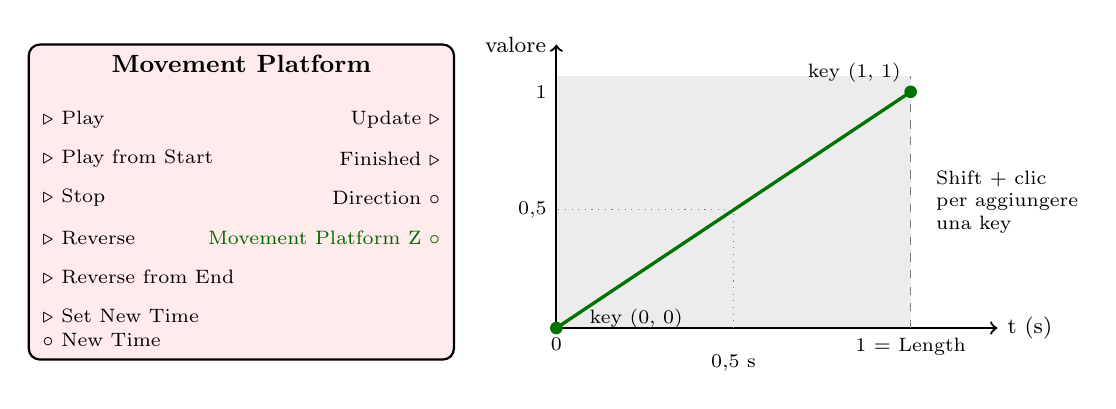
\begin{tikzpicture}[font=\footnotesize,
  ue6tl/.style={draw, thick, rounded corners=4pt, fill=red!8, minimum width=5.4cm,
                minimum height=4.0cm},
  ue6pin/.style={font=\scriptsize}]
  % nodo
  \node[ue6tl] (tl) at (0,0) {};
  \node[font=\small\bfseries] at (0,1.75) {Movement Platform};
  \foreach \t [count=\k] in {Play, Play from Start, Stop, Reverse, Reverse from End,
                             Set New Time} {
    \node[ue6pin, anchor=west] at (-2.65,1.55-0.5*\k) {$\triangleright$ \t};
  }
  \node[ue6pin, anchor=west] at (-2.65,-1.75) {$\circ$ New Time};
  \node[ue6pin, anchor=east] at (2.65,1.05) {Update $\triangleright$};
  \node[ue6pin, anchor=east] at (2.65,0.55) {Finished $\triangleright$};
  \node[ue6pin, anchor=east] at (2.65,0.05) {Direction $\circ$};
  \node[ue6pin, anchor=east, text=green!40!black] at (2.65,-0.45) {Movement Platform Z
    $\circ$};
  % curva
  \begin{scope}[xshift=4.0cm, yshift=-1.6cm]
    \fill[gray!15] (0,0) rectangle (4.5,3.2);
    \draw[->, thick] (0,0) -- (5.6,0) node[right]{t (s)};
    \draw[->, thick] (0,0) -- (0,3.6) node[left]{valore};
    \draw[gray, dashed] (4.5,0) -- (4.5,3.2);
    \node[font=\scriptsize, below] at (4.5,0) {1 = Length};
    \node[font=\scriptsize, below] at (0,0) {0};
    \node[font=\scriptsize, left] at (0,3.0) {1};
    \node[font=\scriptsize, left] at (0,1.5) {0,5};
    \draw[very thick, green!45!black] (0,0) -- (4.5,3.0);
    \fill[green!45!black] (0,0) circle (0.08);
    \fill[green!45!black] (4.5,3.0) circle (0.08);
    \node[font=\scriptsize, right] at (0.3,0.12) {key (0, 0)};
    \node[font=\scriptsize, above left] at (4.5,3.0) {key (1, 1)};
    \draw[gray, dotted] (2.25,0) -- (2.25,1.5) -- (0,1.5);
    \node[font=\scriptsize, align=center] at (2.25,-0.45) {0,5 s};
    \node[font=\scriptsize, align=left, anchor=west] at (4.7,1.6) {Shift + clic\\per
      aggiungere\\una key};
  \end{scope}
\end{tikzpicture}
\caption{Il nodo Timeline della piattaforma e la sua float track. A sinistra i sei
ingressi di esecuzione e le uscite: Update, Finished, Direction e il pin della traccia.
A destra la curva: Length 1 secondo (la zona grigia), due key in (0, 0) e (1, 1); a metà
del tempo il valore è a metà. Schema ricostruito.}
\label{ue6:fig:timeline}
\end{figure}

\begin{table}[htbp]
\centering
\small
\begin{tabular}{@{}p{3.4cm}p{10.6cm}@{}}
\toprule
\textbf{Pin} & \textbf{Che cosa fa} \\
\midrule
Play & riprende dal tempo attuale, in avanti \\
Play from Start & torna a 0 e va in avanti \\
Stop & ferma la timeline dove si trova \\
Reverse & riprende dal tempo attuale, all'indietro \\
Reverse from End & salta alla fine e va all'indietro \\
Set New Time & porta la timeline al tempo New Time \\
\midrule
Update & scatta a ogni aggiornamento mentre la timeline scorre \\
Finished & scatta quando la timeline arriva a un estremo (la fine in avanti, l'inizio
all'indietro) \\
Direction & la direzione attuale: Forward o Backward (un'enumerazione,
\emph{ETimelineDirection}) \\
una uscita per traccia & il valore della traccia al tempo attuale (float, vettore,
colore); le Event track hanno invece un'uscita di esecuzione \\
\bottomrule
\end{tabular}
\caption{I pin del nodo Timeline.}
\label{ue6:tab:timeline}
\end{table}

\paragraph{Approfondimento: le timeline secondo Romero e Sewell.} Nel capitolo 6
(\emph{Enhancing Player Abilities}) i due autori usano una timeline per lo
\emph{zoom} del mirino: una float track \emph{Field of View} da 90 a 45 in 0,3 secondi,
collegata dall'Update al nodo \emph{Set Field of View}, con il tasto premuto su Play e il
tasto rilasciato su \textbf{Reverse}, esattamente lo schema che la lezione userà per la
piattaforma che sale e scende. Il libro aggiunge due osservazioni. La prima: le timeline
sono perfette ``per semplici cambi di valore, come la rotazione di una porta''; per
animazioni complesse, di personaggi o cinematiche, Unreal ha il \textbf{Sequencer}. La
seconda (nella tabella che confronta macro, funzioni ed eventi): i nodi Timeline si
possono usare solo nell'\textbf{Event Graph} di un actor, non dentro le funzioni né
dentro le macro, perché, come i Delay, sono azioni che durano nel tempo. Nelle opzioni
in cima all'editor ci sono poi \textbf{Auto Play} (parte da sola al Begin Play),
\textbf{Loop} (ricomincia all'infinito, utile per un'altalena) e \textbf{Use Last
Keyframe} (fa finire la timeline sull'ultima key invece che alla Length). Le key, con il
tasto destro, possono avere interpolazione lineare, costante o \emph{auto} (curva
morbida, con le tangenti): una curva a ``S'' fa partire e arrivare la piattaforma
dolcemente, invece che di colpo.

% ---------------------------------------------------------------------
\section{L'interpolazione lineare e l'alfa}
\label{ue6:sec:lerp}

``Adesso ci servirebbe fare quello che viene chiamato, in informatica e anche su Unreal,
\textbf{interpolazione}.'' C'è una slide: l'\textbf{interpolazione lineare} ``ci dice:
passo da questo punto a questo punto, passandomi per tutti gli intermedi'', con un
\textbf{alfa}.

\paragraph{L'esempio delle animazioni.} ``L'interpolazione è un concetto che possiamo
trovare in tante cose diverse, tra cui le animazioni.'' Per muovere gli arti di un
personaggio si usano le \textbf{ossa}, interne alla \emph{mesh}. Il docente muove il
braccio davanti alla webcam: ``io non è che vedo subito così, pa!, di scatto: passo
proprio da questo a questo''. ``L'interpolazione è il passaggio per tutti i punti
intermedi che mi fa arrivare alla posizione finale.''

\paragraph{L'alfa.} ``Seguitemi bene attentamente, ragazzi.'' Su una linea che va da 0 a
100, l'alfa è ``un \textbf{puntatore} del punto in cui ci troviamo'', espresso da 0 a 1.
Se siamo a 0, l'alfa è 0; se siamo a 100, l'alfa è 1; ``se l'alfa sta a 0,5, ci
troveremo alla sua metà''. Domanda: se siamo a 20? Uno studente: ``0,2''. ``Ottimo. Siamo
a 0,2: l'alfa sarà a 0,2.'' ``Ci sono varie tipologie di interpolazione, ma
l'interpolazione funziona in questo modo'' (figura~\ref{ue6:fig:lerp}).

\begin{figure}[htbp]
\centering
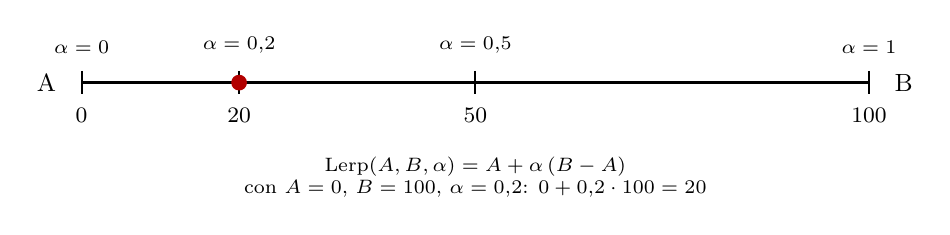
\begin{tikzpicture}[font=\footnotesize]
  \draw[very thick] (0,0) -- (10,0);
  \foreach \x/\l in {0/0, 2/20, 5/50, 10/100} {
    \draw[thick] (\x,0.15) -- (\x,-0.15);
    \node[below] at (\x,-0.2) {\l};
  }
  \node[above, font=\scriptsize] at (0,0.25) {$\alpha = 0$};
  \node[above, font=\scriptsize] at (2,0.25) {$\alpha = 0{,}2$};
  \node[above, font=\scriptsize] at (5,0.25) {$\alpha = 0{,}5$};
  \node[above, font=\scriptsize] at (10,0.25) {$\alpha = 1$};
  \node[left, font=\small] at (-0.2,0) {A};
  \node[right, font=\small] at (10.2,0) {B};
  \fill[red!70!black] (2,0) circle (0.1);
  \node[align=center, font=\scriptsize] at (5,-1.2) {$\mathrm{Lerp}(A, B, \alpha) = A +
    \alpha\,(B - A)$\\con $A = 0$, $B = 100$, $\alpha = 0{,}2$: $0 + 0{,}2 \cdot 100 =
    20$};
\end{tikzpicture}
\caption{L'alfa dell'interpolazione lineare: un numero da 0 a 1 che dice in che punto
del segmento da A a B ci troviamo. L'esempio della lezione: a 20 su 100 l'alfa vale
0,2. La formula, sotto, non è stata scritta a lezione ma è quella che il nodo Lerp
calcola. Schema ricostruito.}
\label{ue6:fig:lerp}
\end{figure}

\paragraph{Approfondimento: Lerp, alfa e timeline.} Il nodo \textbf{Lerp} (per i float)
calcola $A + \alpha(B - A)$: con $\alpha = 0$ restituisce A, con $\alpha = 1$
restituisce B, e in mezzo i valori intermedi in proporzione. Esiste per i vettori
(\textbf{Lerp (Vector)}, che interpola X, Y e Z con lo stesso alfa), per le rotazioni
(\textbf{Lerp (Rotator)}, con l'opzione \emph{Shortest Path}), per i colori e per i
\emph{transform}. L'alfa può anche uscire da $[0, 1]$: con 1,2 il risultato va oltre B
(estrapolazione). Il binomio timeline--Lerp è classico perché divide i compiti: la
\textbf{timeline} decide \emph{come} si scorre nel tempo (quanto dura, con che curva,
avanti o indietro), il \textbf{Lerp} decide \emph{dove} si va (da A a B). Cambiare la
durata o la forma del movimento non tocca A e B, e viceversa. Da non confondere con i nodi
\emph{FInterp To} e \emph{RInterp To} (quest'ultimo usato per la torretta): quelli
avvicinano ogni frame un valore al bersaglio di una frazione, con una velocità e il
Delta Time, senza un alfa né una durata fissa.

% ---------------------------------------------------------------------
\section{Il primo metodo: un Lerp sulla Z}
\label{ue6:sec:metodo1}

``Abbiamo quindi da tirare fuori il nostro bellissimo \textbf{Lerp}.'' Domanda di
partenza, guardando la piattaforma: ``quale asse dovremmo influenzare, che si muova nel
tempo?'' ``La Z.'' ``Ottimo, bravo, Federico.''

\paragraph{La costruzione.} Il docente procede per tentativi, e a un certo punto uno
studente chiede: ``potresti spiegare un po' tutti i passaggi? Perché a un certo punto mi
sono perso''. La versione rispiegata, che è quella da seguire, è questa
(figura~\ref{ue6:fig:metodo1}).
\begin{enumerate}
  \item Si prende il componente \textbf{Platform} e si tira fuori \textbf{Get Relative
        Location}. All'inizio il docente aveva usato Get Actor Location, poi la World
        Location (``scusate, ragazzi, questa è world''), e infine la \emph{relative},
        cioè la posizione rispetto all'actor. Si splitta il vettore.
  \item La \textbf{Z} relativa va, da sola, nel pin \textbf{A} del Lerp: il punto di
        partenza.
  \item La stessa Z più una variabile float nuova, \textbf{MaxHeight}, va nel pin
        \textbf{B}: il punto d'arrivo. Il valore scelto è \textbf{70} (``ci piace 70'';
        ``sono 70 unità sulla Z'').
  \item L'\textbf{Alpha} del Lerp è il pin \textbf{Movement Platform Z} della timeline.
  \item Un \textbf{Make Vector}: X e Y dalla location relativa, invariate; Z dal Lerp.
  \item \textbf{Set Relative Location} sul componente Platform, con il Make Vector nel
        pin \emph{New Location}, eseguito dall'\textbf{Update} della timeline.
\end{enumerate}
La timeline parte dal Begin Overlap della box, attraverso il Branch sul player, con
\textbf{Play}.

\begin{figure}[htbp]
\centering
\begin{tikzpicture}[font=\footnotesize,
  ue6node/.style={draw, thick, rounded corners=4pt, align=center, fill=gray!8,
                  minimum height=0.8cm, text width=2.1cm},
  ue6event/.style={ue6node, fill=red!12},
  ue6exec/.style={-{Stealth[length=2.5mm]}, very thick, black!80},
  ue6data/.style={-{Stealth[length=2mm]}, thick, green!45!black},
  ue6vec/.style={-{Stealth[length=2mm]}, thick, yellow!50!black}]
  \node[ue6event, text width=2.5cm] (ov) at (0,0) {\textbf{On Component Begin
    Overlap} (Box)};
  \node[ue6node, text width=2.4cm] (eq) at (0,-1.8) {Other Actor \textbf{==}\\\textbf{Get
    Player Pawn}};
  \node[ue6node, text width=1.3cm] (br) at (3.0,0) {\textbf{Branch}};
  \node[ue6node, text width=2.3cm] (tl) at (5.8,0) {\textbf{Timeline}\\Movement
    Platform};
  \node[ue6node, text width=2.4cm] (set) at (11.0,0) {\textbf{Set Relative
    Location}\\(Platform)};
  \node[ue6node, text width=2.5cm] (grl) at (3.0,-3.6) {Platform $\rightarrow$
    \textbf{Get Relative Location} (split)};
  \node[ue6node, text width=1.8cm] (mh) at (5.8,-3.6) {Z +\\\textbf{MaxHeight} (70)};
  \node[ue6node, text width=1.4cm] (lerp) at (8.2,-2.0) {\textbf{Lerp}\\A, B, Alpha};
  \node[ue6node, text width=1.7cm] (mv) at (11.0,-2.0) {\textbf{Make Vector}};
  \draw[ue6exec] (ov) -- (br);
  \draw[ue6exec] (br) -- node[above, font=\scriptsize]{True} node[below,
    font=\scriptsize]{Play} (tl);
  \draw[ue6exec] (tl) -- node[above, font=\scriptsize]{Update} (set);
  \draw[-{Stealth[length=2mm]}, thick, red!60!black] (eq.north) -- node[right,
    font=\scriptsize]{bool} (br.south west);
  \draw[ue6data] (tl.south) -- node[left, font=\scriptsize, pos=0.3]{Z track} (lerp.west);
  \draw[ue6data] (grl.north) |- node[pos=0.25, left, font=\scriptsize]{Z $\rightarrow$ A}
    ([yshift=-0.2cm]lerp.west);
  \draw[ue6data] (grl) -- (mh);
  \draw[ue6data] (mh.east) -| node[pos=0.7, right, font=\scriptsize]{B} (lerp.south);
  \draw[ue6data] (lerp) -- node[above, font=\scriptsize]{Z} (mv);
  \draw[ue6data] (grl.south) -- ++(0,-0.35) -| node[pos=0.25, below,
    font=\scriptsize]{X, Y} (mv.south);
  \draw[ue6vec] (mv) -- node[right, font=\scriptsize]{New Location} (set);
\end{tikzpicture}
\caption{Il primo metodo. Il Begin Overlap della box, se l'actor è il player, fa
partire la timeline; a ogni Update un Lerp tra la Z relativa attuale (A) e la stessa Z
più MaxHeight (B), con la traccia della timeline come alfa, diventa la nuova Z della
Platform. Funziona, ma ha un difetto: A e B vengono riletti a ogni Update dalla posizione
già spostata (vedi l'approfondimento). Schema ricostruito.}
\label{ue6:fig:metodo1}
\end{figure}

\paragraph{``Va altissimo''.} In Play la piattaforma sale, ma molto più di 70 unità: a uno
studente, con 70, ``arriva in cielo''; con 30 arriva ``poco più alto del muretto'' della
scena. ``Non so perché, però sia così diverso.'' Il docente promette un metodo ``un po'
più carino e più malleabile''; la spiegazione arriva, in parte, dopo la pausa: ``stiamo
sommando'' (sezione~\ref{ue6:sec:playrate}).

\paragraph{Approfondimento: perché il primo metodo ``somma''.} A ogni Update il grafo
legge la Z \emph{attuale} della Platform, che è già stata spostata dall'Update
precedente, e la usa come A; B è quella Z più 70. Il risultato è quindi
$Z_{\text{nuova}} = Z_{\text{attuale}} + \alpha \cdot 70$: non un punto tra due estremi
fissi, ma un \emph{incremento} che si accumula. Se la timeline si aggiorna $N$ volte in
un secondo, la piattaforma sale di circa $70 \cdot \sum \alpha_k \approx 70 \cdot N/2$
unità: con 60 aggiornamenti al secondo, più di duemila, non settanta. Da qui tre
conseguenze, tutte osservate a lezione. La salita dipende dal \emph{frame rate} (``è la
mia impressione che vada più in alto'': su un computer più veloce, più somme). Rallentare
la timeline con il play rate fa \emph{più} somme, e la piattaforma sale ancora di più;
accelerarla ne fa meno. E con il Reverse il calcolo non torna simmetrico: lo studente
che si vedeva la piattaforma ``sempre leggermente più in basso fino a scomparire sotto il
terreno'' stava osservando proprio l'errore che si accumula a ogni salita e discesa. La
cura è leggere A e B \emph{una volta sola}, prima che la timeline parta, e tenerli fissi:
è il secondo metodo.

% ---------------------------------------------------------------------
\section{La pausa e il Nintendo Direct}
\label{ue6:sec:pausa}

``Sono le 17:37. Facciamo la pausa classica di 20 minuti''; si torna ``alle 18''. Durante
la pausa il docente aiuta uno studente con la foto del codice mandata su Discord (il
problema è l'altezza della piattaforma con il primo metodo: ``70 è giusto'', il resto
``credo sia tutto giusto''), e poco prima della ripresa arrivano le notizie dal
\emph{Nintendo Direct}, riferite da uno studente ``referente''. Nella trascrizione,
molto storpiata, si riconoscono un \emph{remake} di \emph{Ocarina of Time} (``l'Opera of
Time Remake''), un nuovo \emph{Xenoblade}, un \emph{Final Fantasy} in 2D-HD ``stile
\emph{Octopath Traveler}'' e del materiale nuovo su \emph{Deltarune}; il tutto è riportato
come lo si legge nella trascrizione, senza verifiche. La chiacchierata scivola su
\emph{Kingdom Hearts} e sulla trilogia \emph{remake} di \emph{Final Fantasy VII} (``uscirà
prima l'intera trilogia remake''), e su Tetsuya Nomura (``le nomurate''). ``Comunque,
sempre belli questi siparietti'', dice il docente; chi segue in differita può
partecipare alla conversazione su Discord, ``pacificamente''.

% ---------------------------------------------------------------------
\section{La velocità della timeline: Set Play Rate e Duration}
\label{ue6:sec:playrate}

``Allora riprendiamo la nostra bellissima \emph{elevator}, o piattaforma, quello che
vogliamo.'' Una cosa che si può controllare è il \textbf{play rate}: ``la velocità in cui
essa, sempre ripetendo un secondo, viene detta: vai a due volte la tua velocità, a metà
della tua velocità''.

\paragraph{La timeline è un componente.} ``Se avete notato'', nel pannello
\textbf{Components} del Blueprint, accanto a Box, Platform e DefaultSceneRoot, c'è anche
\textbf{Movement Platform}: ``lo stesso nome della timeline''. Ogni timeline aggiunta
crea un componente con il suo nome, e da quel componente si possono chiamare le sue
funzioni. Trascinandolo nel grafo (``Ctrl per il Get''), se ne tira fuori \textbf{Set
Play Rate}, con il \emph{Target} sulla timeline.

\paragraph{Play rate e lunghezza.} Sul \textbf{Begin Play}, Set Play Rate a 0,5: ``la
sua velocità sarà la metà''; a 2, ``il doppio''; a 1, ``andrà come prima''. Il docente
insiste: ``il play rate \textbf{non è la lunghezza}, non è la Length, è diversa''. La
Length dice quanto è lunga la curva; il play rate dice quanto velocemente la si
percorre.

\paragraph{Il primo metodo non regge.} Con il play rate cambiato, la piattaforma del primo
metodo si comporta in modo strano, e il docente ne dà la spiegazione: ``stiamo
aumentando di 30 a ogni frame del nostro secondo''; ``se riduciamo il play rate, lui
sarà più veloce, ma di conseguenza farà meno somme''. Detto meglio: con un play rate più
alto la timeline finisce prima, fa meno Update, e quindi meno somme; con uno più basso ne
fa di più. ``Vedete che non si ferma a quell'unità, perché in questo caso stiamo sommando
solamente: se finisce prima, vuol dire che finirà prima.''

\paragraph{La variabile Duration.} Ragionare in velocità relative è scomodo; è più
naturale dire ``voglio che duri 2 secondi''. Una variabile float \textbf{Duration} e un
piccolo calcolo:
\[
  \text{Play Rate} = \frac{1}{\text{Duration}} \times \text{Timeline Length},
\]
con \textbf{Divide} (``lo slash'') e \textbf{Get Timeline Length} (dal componente della
timeline) moltiplicati con \textbf{Multiply}, e il risultato nel Set Play Rate del Begin
Play. Con Duration 1 e una Length di 1 il play rate è 1, ``velocità normale''. Con
Duration 2 il docente prima dice ``il doppio'', poi si corregge: ``no, scusa, sarà più
lunga, perdonate''; con 0,5 sarà più veloce. È ``una variabile d'appoggio'' che traduce
una durata in secondi nel play rate giusto. Per il resto della lezione la Duration resta
a 1, ``così almeno siamo tranquilli''.

\paragraph{Approfondimento: perché la formula funziona.} Una timeline di lunghezza $L$
percorsa con play rate $r$ dura $L / r$ secondi. Volendo che duri $D$ secondi, basta
porre $L / r = D$, cioè $r = L / D$: è la formula del docente, scritta come $1/D \times
L$. Moltiplicare per la Length rende il calcolo indipendente dalla curva: se un giorno la
timeline diventa lunga 3 secondi, la Duration continua a dire la durata vera. Due
cautele. Una Duration a 0 produce una divisione per zero, e la timeline non si muove più
(il primo sospetto, a lezione, quando la piattaforma di uno studente ``ha smesso di
muoversi''). E il Set Play Rate va chiamato sulla timeline \emph{giusta}: è l'errore
della sezione~\ref{ue6:sec:timelinesbagliata}.

% ---------------------------------------------------------------------
\section{Il secondo metodo: il Billboard e le posizioni salvate}
\label{ue6:sec:metodo2}

Per avere ``due punti specifici da raggiungere, in modo non dipendente da dei valori'',
il docente rifà il grafo. Il vecchio si può tenere, staccato, e copiare (``Ctrl+C,
Ctrl+V'') i pezzi che servono; il Set Relative Location della Platform resta: ``non lo
cancellate, perché è giusto che sia così''.

\paragraph{Il Billboard.} Si aggiunge (\emph{Add}) un componente \textbf{Billboard}:
``un oggetto di questo tipo: è questo \textbf{dinosauro}''. ``Fondamentalmente è un punto
nello spazio'', come lo \emph{Scene Component} già usato per la torretta; ``la
differenza è che ha un'immagine'', visibile solo nell'editor. Il piano: ``prendere la sua
posizione nello spazio, e dire: \emph{lerpami} da questa posizione della piattaforma
iniziale a questa posizione del billboard''. Il Billboard si mette a \textbf{500} sulla
Z (``o di più? 700? Mettete 500, la metà è giusta'').

\paragraph{Lerp (Vector).} Al posto del Lerp sui float, un \textbf{Lerp (Vector)} (``un
v-lerp, un lerp tra vettori''): ``invece che tra due numeri, due float, tra due
vettori''. A è la \textbf{Get Relative Location} della Platform, B quella del Billboard,
l'Alpha la traccia della timeline; l'uscita va direttamente nel Set Relative Location
della Platform, senza Make Vector.

\paragraph{``C'è qualcosa di sbagliato?''} Così com'è, avverte il docente, il grafo ha
ancora il difetto del primo metodo: ``non salviamo mai la posizione delle due''. Se il
Billboard fosse \textbf{attaccato} alla Platform, ``si muoverà insieme ad essa'', e
allora ``avremo un effetto infinito'': la piattaforma insegue un bersaglio che si
allontana, ``un continuo movimento sempre in alto, sempre in alto, pom pom pom''. Il
docente lo mostra riattaccando il Billboard: ``e si ricomincia''. La cura:
\begin{enumerate}
  \item i due Get Relative Location si spostano sul \textbf{Begin Play};
  \item sul pin di uscita di ciascuno, \textbf{Promote to Variable}: la Platform diventa
        \textbf{StartLocation}, il Billboard \textbf{FinishLocation};
  \item nel Lerp (Vector) entrano i \emph{Get} delle due variabili: StartLocation in A,
        FinishLocation in B.
\end{enumerate}
``Così facendo abbiamo delle variabili che sono sempre fisse'': ``sarà sempre la stessa
posizione'' (figura~\ref{ue6:fig:metodo2}).

\paragraph{Il bello del Billboard.} ``La cosa bella, poi, che possiamo vedere con questo
metodo'': il dinosauro si può spostare nello spazio, nei dettagli della piattaforma, e la
piattaforma raggiungerà quel punto. ``Dovete fare un livello? L'avete alzato a 8 metri?
Prendete il billboard, lo mettete a 800'': ``devo arrivare qua sopra, quindi arriverò
qua. Ecco fatto, sono arrivato preciso''. (``Salto, l'ho mancato malissimo.'') E non solo
in verticale: spostando il Billboard anche sulla X o sulla Y, ``andrà in diagonale'';
``potremmo pure fare piattaforme in orizzontale, in diagonale, come vi pare''. ``Invece
di fare matematica'', si prendono direttamente i due vettori.

\paragraph{Il ritorno: Reverse.} Scendendo dalla piattaforma, questa ``rimane là''.
``Vi potrei dire: facciamo una nuova timeline e la facciamo al contrario. Non serve.
Perché abbiamo \textbf{Reverse}.'' L'\textbf{On Component End Overlap} della box,
collegato al pin Reverse della timeline: ``esco fuori e lei se ne torna al suo posto'',
perché ``invece di fare da A a B, fa da B ad A. Questo è insito nella timeline''.

\begin{figure}[htbp]
\centering
\begin{tikzpicture}[font=\footnotesize,
  ue6node/.style={draw, thick, rounded corners=4pt, align=center, fill=gray!8,
                  minimum height=0.8cm, text width=2.1cm},
  ue6event/.style={ue6node, fill=red!12},
  ue6var/.style={ue6node, fill=blue!10, rounded corners=8pt},
  ue6exec/.style={-{Stealth[length=2.5mm]}, very thick, black!80},
  ue6data/.style={-{Stealth[length=2mm]}, thick, green!45!black},
  ue6vec/.style={-{Stealth[length=2mm]}, thick, yellow!50!black}]
  % Begin Play
  \node[ue6event, text width=2.4cm] (bp) at (0,0) {\textbf{Event Begin Play}};
  \node[ue6node, text width=2.3cm] (s1) at (3.3,0) {\textbf{Set}\\StartLocation};
  \node[ue6node, text width=2.3cm] (s2) at (6.4,0) {\textbf{Set}\\FinishLocation};
  \node[ue6node, text width=2.2cm] (pr) at (9.6,0) {\textbf{Set Play Rate}\\($1/D \times
    L$)};
  \node[ue6node, text width=2.5cm] (g1) at (3.3,-1.6) {Platform $\rightarrow$ Get
    Relative Location};
  \node[ue6node, text width=2.5cm] (g2) at (6.4,-1.6) {Billboard $\rightarrow$ Get
    Relative Location};
  \draw[ue6exec] (bp) -- (s1);
  \draw[ue6exec] (s1) -- (s2);
  \draw[ue6exec] (s2) -- (pr);
  \draw[ue6vec] (g1) -- (s1);
  \draw[ue6vec] (g2) -- (s2);
  % overlap e timeline
  \begin{scope}[yshift=-3.6cm]
    \node[ue6event, text width=2.6cm] (bo) at (-0.2,0) {\textbf{Begin Overlap}
      (Box)\\+ Branch sul player};
    \node[ue6event, text width=2.6cm] (eo) at (-0.2,-1.5) {\textbf{End Overlap} (Box)};
    \node[ue6node, text width=2.2cm, minimum height=2.2cm] (tl) at (3.6,-0.75)
      {\textbf{Timeline}\\Movement\\Platform};
    \node[ue6node, text width=1.9cm] (lv) at (7.0,-2.5) {\textbf{Lerp (Vector)}\\A, B,
      Alpha};
    \node[ue6var, text width=1.9cm] (v1) at (7.0,-4.0) {StartLocation};
    \node[ue6var, text width=2.1cm] (v2) at (9.8,-4.0) {FinishLocation};
    \node[ue6node, text width=2.4cm] (set) at (10.4,-0.4) {\textbf{Set Relative
      Location}\\(Platform)};
    \draw[ue6exec] (bo.east) -- node[above, font=\scriptsize]{Play} ([yshift=0.75cm]tl.west);
    \draw[ue6exec] (eo.east) -- node[below, font=\scriptsize]{Reverse}
      ([yshift=-0.75cm]tl.west);
    \draw[ue6exec] ([yshift=0.35cm]tl.east) -- node[above, font=\scriptsize]{Update}
      (set.west);
    \draw[ue6data] ([yshift=-0.6cm]tl.east) -| node[pos=0.25, above,
      font=\scriptsize]{Alpha} (lv.north);
    \draw[ue6vec] (v1) -- node[left, font=\scriptsize]{A} (lv);
    \draw[ue6vec] (v2.north) |- node[pos=0.25, right, font=\scriptsize]{B} (lv.east);
    \draw[ue6vec] (lv.east) -- ++(0.9,0) |- node[pos=0.2, right,
      font=\scriptsize]{New Location} (set.south west);
  \end{scope}
\end{tikzpicture}
\caption{Il secondo metodo. Sopra: al Begin Play le posizioni relative della Platform e
del Billboard vengono salvate una volta per tutte in StartLocation e FinishLocation (con
Promote to Variable), e si imposta il play rate dalla Duration. Sotto: il Begin Overlap
fa Play, l'End Overlap fa Reverse; a ogni Update un Lerp (Vector) tra i due punti fissi,
con la traccia come alfa, diventa la nuova posizione della Platform. Schema
ricostruito.}
\label{ue6:fig:metodo2}
\end{figure}

\paragraph{I problemi.} ``Problemi su questo? Siete a posto?'' Tre casi.
\begin{itemize}
  \item \textbf{``A me non si muove.''} Il docente ripassa la lista: le due Get Relative
        Location, le due variabili, la timeline in Play, l'Update, il Lerp tra i
        vettori, l'Alpha collegato. Lo studente non aveva capito come creare le
        variabili: tasto destro sul pin, \textbf{Promote to Variable}, e il nome. Poi
        StartLocation in A, FinishLocation in B, e l'Alpha alla traccia della timeline.
  \item \textbf{L'evento diventato Custom Event.} Uno studente scopre da solo il suo
        errore: copiando e incollando il blocco, l'evento di overlap ``mi ha preso come
        Custom Event generico, e quindi non si muoveva''. Un evento di componente
        incollato in un Blueprint perde il legame con il componente e diventa un evento
        qualunque, che nessuno chiama. ``Errore di distrazione.''
  \item \textbf{Ero rimasto indietro.} Uno studente, che aveva ricevuto una telefonata,
        riceve il riassunto: Billboard, Get Relative Location della Platform in
        StartLocation e del Billboard in FinishLocation, il Lerp (Vector) con l'alfa, il
        Set Relative Location, e il Reverse sull'End Overlap.
\end{itemize}

\paragraph{Approfondimento: Billboard figlio di chi?} Il docente fa vedere che, con il
Billboard attaccato alla Platform, la piattaforma ``sale all'infinito'', e che salvando le
posizioni al Begin Play il problema scompare. Ma c'è un dettaglio che la lezione non
esplicita: se il Billboard resta figlio della Platform, la sua \emph{relative location}
è relativa alla Platform, non all'actor; salvarla al Begin Play dà $(0, 0, 500)$ rispetto
alla piattaforma, mentre il Set Relative Location della Platform lavora rispetto alla
radice dell'actor. I due numeri coincidono solo se la Platform sta nell'origine
dell'actor (come nel Blueprint della lezione). La configurazione più robusta è mettere il
Billboard come figlio della \textbf{DefaultSceneRoot}, accanto alla Platform, così che
le due posizioni relative siano nello stesso spazio e il bersaglio non si muova mai con
la piattaforma. Un'altra soluzione, equivalente, è salvare e impostare le posizioni nel
mondo (Get e Set World Location). Infine: il ``dinosauro'' è visibile solo nell'editor;
nel gioco il Billboard non si vede, come tutti i componenti di servizio.

% ---------------------------------------------------------------------
\section{La timeline sbagliata}
\label{ue6:sec:timelinesbagliata}

Il docente vuole far vedere che la Duration funziona anche con il secondo metodo: ``la
cambio in 2''; poi, ``mettiamo dei valori che posso riconoscere, tipo 10''. Ma la
velocità non cambia. ``Non mi setta il play rate, forse.'' Anche a uno studente,
``l'unica cosa è la duration: non va effettivamente a modificare la velocità''. Il
docente prova un Print, un play rate a 0,1, a mille: ``sempre lo stesso''.

\paragraph{La soluzione, da uno studente.} ``Domanda un po' stupida: non è che forse
l'attore deve essere Platform e non Movement Platform?'' Non è quello, ma è la pista
giusta: ``errore mio''. Il secondo metodo usa una timeline \emph{nuova}, che si chiama
semplicemente \textbf{Timeline}; il Set Play Rate del Begin Play aveva come Target ancora
\textbf{Movement Platform}, ``quella dell'esempio di prima''. ``Stavamo referenziando la
timeline dell'altro esempio, e non la playavamo mai.''

\paragraph{La lezione dell'errore.} ``Da questo errore possiamo imparare qualche cosa'':
``le timeline hanno un \textbf{nome}''. Ogni timeline è un componente distinto, e le sue
funzioni (Set Play Rate, Get Timeline Length, Play, Reverse\ldots) agiscono solo su di
lei. Con il Target giusto e una Duration di 3, la piattaforma ``adesso è più lenta,
perché dura di più''. Morale: dare alle timeline nomi chiari, e cancellare quelle che non
servono più.

% ---------------------------------------------------------------------
\section{L'audio: la Sound Cue}
\label{ue6:sec:cue}

``Se non ci sono più problemi, passiamo al nostro bellissimo \emph{sound}.''

\paragraph{Importare il file.} Un consiglio d'ordine: una \textbf{cartella audio} nel
Content Browser (tasto destro, \emph{New Folder}). Per importare il file scaricato da
Discord basta \textbf{trascinarlo} nel Content Browser: appare un asset ``con la linea'',
una \textbf{Sound Wave}, senza altre domande.

\paragraph{Creare la Cue.} Sulla Sound Wave, tasto destro, \textbf{Create Cue} (``è il
secondo''). La \textbf{Sound Cue} (``la queue'', ``la Q'', nella trascrizione) è, dice il
docente, ``un \emph{sound} programmabile, tra virgolette''. Doppio clic: si apre un grafo
``come abbiamo visto anche su Unreal molto spesso'', con un nodo \textbf{Wave Player}
(il nostro suono) collegato all'\textbf{Output}. A sinistra, i dettagli della Cue:
\textbf{Volume Multiplier}, \textbf{Pitch Multiplier}, \emph{Sound Class} (``class
override''), \emph{Attenuation} e così via, ``tutti i vari dati che possiamo
modificare''.

\paragraph{Il pitch.} Con il Pitch Multiplier a 2 il suono è più alto; a 0,5 ``è pitchato
verso il basso'': ``molto più basso livello di tono, e anche più lento''. ``Perché il
pitch influenza sia la velocità sia la tonalità.'' Si torna a 1.

\paragraph{Il loop.} Con Play il suono parte ``solo una volta''; ``noi vogliamo che vada
in loop'' finché la piattaforma si muove, ``tipo: pipi, pipi, pipi''. Sul nodo
\textbf{Wave Player} si spunta \textbf{Looping}. (``Ovviamente rompe'': con la barra
spaziatrice si avvia e si interrompe l'anteprima.)

\paragraph{Il Modulator.} ``Vogliamo che magari il pitch o il volume siano un valore
\textbf{randomico}, tra un valore e un altro, in modo che non sia sempre lo stesso
suono.'' Si inserisce un nodo \textbf{Modulator} tra il Wave Player e l'Output: ha
\textbf{Pitch Min}, \textbf{Pitch Max}, \textbf{Volume Min} e \textbf{Volume Max}. I
valori della lezione: pitch tra \textbf{1,7} e \textbf{2}, volume tra \textbf{1} e
\textbf{1,2}. A ogni riproduzione il suono è ``leggermente più basso, leggermente più
alto''. Il perché, con il gioco della palla del docente: quando rimbalza fa un
\emph{boing}, ``e visto che avevo solo un suono'', che ripetuto ``sembra la stessa
cosa'', un pitch minimo e massimo hanno dato ``un risultato molto più gradevole''.

\paragraph{Il Random.} ``Esiste anche il \textbf{Random}'': se si hanno più suoni, il
nodo Random ne sceglie uno a caso a ogni riproduzione. Il docente lo prova mettendo nel
Random due rami, uno con il Modulator e uno senza, e ascoltando quale esce. L'uso tipico:
``un proiettile che prende un muro: invece di avere sempre lo stesso suono, mettete tutti
e tre i suoni nel Random''. Per la piattaforma non serve, e si torna al solo Modulator
(figura~\ref{ue6:fig:cue}).

\begin{figure}[htbp]
\centering
\begin{tikzpicture}[font=\footnotesize,
  ue6snode/.style={draw, thick, rounded corners=4pt, align=center, fill=violet!10,
                   minimum height=1.0cm, text width=2.5cm},
  ue6out/.style={draw, thick, rounded corners=4pt, align=center, fill=gray!20,
                 minimum height=1.0cm, text width=1.6cm},
  ue6aud/.style={-{Stealth[length=2.5mm]}, very thick, violet!60!black}]
  \node[ue6snode] (wp) at (0,0) {\textbf{Wave Player}\\SFX Moving Platform\\Looping
    \checkmark};
  \node[ue6snode] (mod) at (4.0,0) {\textbf{Modulator}\\Pitch 1,7--2\\Volume 1--1,2};
  \node[ue6out] (out) at (7.6,0) {\textbf{Output}};
  \draw[ue6aud] (wp) -- (mod);
  \draw[ue6aud] (mod) -- (out);
  \node[draw, dashed, rounded corners=4pt, align=left, text width=4.6cm, font=\scriptsize]
    at (11.4,0) {dettagli della Cue: Volume Multiplier, Pitch Multiplier (1), Sound
    Class, Attenuation\ldots};
  % variante random
  \begin{scope}[yshift=-2.4cm]
    \node[ue6snode, text width=2.0cm] (w1) at (0,0.6) {Wave Player 1};
    \node[ue6snode, text width=2.0cm] (w2) at (0,-0.6) {Wave Player 2};
    \node[ue6snode, text width=1.6cm] (rnd) at (4.0,0) {\textbf{Random}};
    \node[ue6out] (out2) at (7.6,0) {\textbf{Output}};
    \draw[ue6aud] (w1.east) -- (rnd.west);
    \draw[ue6aud] (w2.east) -- (rnd.west);
    \draw[ue6aud] (rnd) -- (out2);
    \node[align=left, font=\scriptsize, text width=4.6cm] at (11.4,0) {variante: più
      suoni, uno scelto a caso a ogni riproduzione (l'esempio del proiettile contro il
      muro)};
  \end{scope}
\end{tikzpicture}
\caption{La Sound Cue della piattaforma: il Wave Player in loop, un Modulator che varia
a caso pitch e volume a ogni riproduzione, l'Output. Sotto, la variante con il nodo
Random mostrata a lezione e poi scartata. Schema ricostruito.}
\label{ue6:fig:cue}
\end{figure}

\paragraph{Approfondimento: Sound Wave, Sound Cue, MetaSound.} La \textbf{Sound Wave} è
il file audio importato, con poche proprietà proprie (fra cui un suo \emph{Looping}). La
\textbf{Sound Cue} è un piccolo grafo che combina una o più Wave con nodi di
elaborazione: Modulator, Random, \emph{Mixer}, \emph{Concatenator}, \emph{Delay},
\emph{Attenuation}\ldots; nei Blueprint si può passare indifferentemente una Wave o una
Cue a qualunque nodo che vuole un \emph{Sound}. In Unreal Engine 5 esistono anche i
\textbf{MetaSound}, un sistema più recente e più potente, che genera e manipola l'audio
con un grafo simile a quello dei Blueprint; le Sound Cue restano supportate e sono il
punto di partenza più semplice. Il formato \textbf{WAV} raccomandato dal docente è quello
standard per l'import: non compresso, lo comprime poi l'engine secondo la piattaforma.
Sul pitch, l'osservazione del docente è esatta: in una Sound Cue il Pitch Multiplier
cambia la velocità di riproduzione, quindi alza o abbassa il tono e accorcia o allunga il
suono insieme, come un disco suonato a giri sbagliati.

% ---------------------------------------------------------------------
\section{Far suonare la piattaforma: Spawn Sound, Do Once e Stop}
\label{ue6:sec:suono}

``Abbiamo due modi per piazzare i suoni'': i nodi \textbf{Play Sound 2D} e \textbf{Play
Sound at Location}, e i nodi \textbf{Spawn Sound 2D} e \textbf{Spawn Sound at Location}.
``La differenza sostanziale è che uno \emph{playa} il suono solamente; l'altro lo
\emph{spawna}, e quindi crea una \textbf{referenza}'', come lo Spawn Actor from Class
``che quando spawna ha un Return Value''.

\paragraph{La prova con Play Sound 2D.} ``Proviamo a mettere Play Sound 2D'': la Cue
nel pin Sound, l'esecuzione dall'Update della timeline. Il docente sale sulla piattaforma: il suono parte,
``e non smette più''. Peggio: l'Update scatta a ogni aggiornamento, quindi i suoni si
sovrappongono (``come avete sentito, è stato uno stormo di uccelli incredibile''). Due
problemi, due soluzioni.
\begin{itemize}
  \item Il suono è in loop: per fermarlo bisogna sapere \emph{quale} suono fermare, e il
        Play Sound non lo dice. Serve lo \textbf{Spawn Sound at Location}, che
        restituisce la referenza.
  \item L'Update scatta molte volte: serve un \textbf{Do Once}, ``che lo fa una sola
        volta''.
\end{itemize}

\paragraph{Lo spawn.} \textbf{Do Once}, poi \textbf{Spawn Sound at Location}: Sound la
Cue, Location la \textbf{Get Actor Location} (``alla locazione dell'attore playerà questo
suono''; il docente pensa prima alla piattaforma, poi sceglie l'actor). Dal \textbf{Return
Value}, \textbf{Promote to Variable}: \textbf{SoundPlatform}. ``Adesso, di questo suono
che abbiamo creato, abbiamo la referenza: qualcosa che punta e ci dice: ehi, questo è il
suono che fa pipipipi.''

\paragraph{Lo stop.} ``Io voglio che si fermi quando la timeline finisce'', cioè quando
arriva in cima (a 1) o torna alla base (a 0). Sul \textbf{Finished} della timeline: Get
di SoundPlatform, \textbf{Stop}. ``Fino a che non è arrivato in cima, o fino a che non è
tornato alla base, il suono playerà, e si stopperà appena finisce la timeline.''

\paragraph{Il Reset del Do Once.} ``Un'ultima cosa molto importante.'' Il Do Once, una
volta passato, resta chiuso; ha però un ingresso \textbf{Reset}: ``se lo inserisco là
dentro, questo Do Once si resetta, si apre, e dà la possibilità di essere rieseguito''.
``Quando ho stoppato il suono una volta, lo devo riattivare per la volta dopo'': dopo lo
Stop, il Reset. ``E si ferma; scendo, ed eccolo. Benissimo.''

% ---------------------------------------------------------------------
\section{Il pitch che cambia con la direzione}
\label{ue6:sec:pitch}

``Potremmo anche, ipoteticamente\ldots'' L'idea: un suono \textbf{più alto quando la
piattaforma sale} e \textbf{più basso quando scende}. Il componente audio spawnato ha la
funzione \textbf{Set Pitch Multiplier}, da chiamare sulla referenza SoundPlatform.

\paragraph{Come sapere se sale o scende.} Il docente comincia a ragionare con un Branch
(``se sta andando da StartLocation a FinishLocation\ldots''), poi si ferma: ``possiamo
usare una cosa molto interessante''. Il pin \textbf{Direction} della timeline è
un'\textbf{enumerazione} (``che vedremo in seguito che cos'è, ma oggi ci serve
semplicemente vedere questa cosa''): ``una variabile che ha dentro di sé due elementi'',
\emph{Forward} e \emph{Backward}. Tirandone fuori uno \textbf{Switch on
ETimelineDirection} si ottengono due uscite di esecuzione: ``avanti vuol dire che sta
andando 0--1, e indietro è 1--0''.
\begin{itemize}
  \item \textbf{Forward}: Set Pitch Multiplier su SoundPlatform a \textbf{1}, il pitch
        normale;
  \item \textbf{Backward}: Set Pitch Multiplier a \textbf{0,4}, ``per far puh, puh, puh,
        un po' più bassino: una discesa'' (il docente prova anche 0,5 e 0,1, ``molto
        basso''; il valore finale è 0,4).
\end{itemize}
``Mettiamo tutto nel Do Once'' (figura~\ref{ue6:fig:suono}).

\paragraph{L'errore dell'ordine.} A una studentessa il grafo, ``sulla carta'', è giusto,
ma il compilatore segnala un errore: il Set Pitch Multiplier dice che il suono ``non è
mai stato creato''. Il motivo è l'ordine: lo Switch, con i due Set Pitch Multiplier,
veniva eseguito \emph{prima} che lo Spawn Sound avesse riempito la variabile, quindi su
una referenza vuota. ``Metti prima il Do Once'', e dopo lo spawn e il Set della
variabile, lo Switch con i due rami. ``Dovrebbe andare.'' E va (dopo aver condiviso anche
l'audio del computer su Zoom, per farlo sentire).

\begin{figure}[htbp]
\centering
\begin{tikzpicture}[font=\footnotesize,
  ue6node/.style={draw, thick, rounded corners=4pt, align=center, fill=gray!8,
                  minimum height=0.8cm, text width=2.0cm},
  ue6var/.style={ue6node, fill=blue!10, rounded corners=8pt},
  ue6exec/.style={-{Stealth[length=2.5mm]}, very thick, black!80},
  ue6data/.style={-{Stealth[length=2mm]}, thick, violet!60!black}]
  \node[ue6node, text width=2.0cm, minimum height=2.0cm] (tl) at (0,0)
    {\textbf{Timeline}};
  \node[ue6node, text width=1.5cm] (do) at (3.4,0.6) {\textbf{Do Once}};
  \node[ue6node, text width=2.4cm] (sp) at (6.1,0.6) {\textbf{Spawn Sound at
    Location}\\Cue, Get Actor Location};
  \node[ue6var, text width=2.1cm] (sv) at (9.1,0.6) {\textbf{Set}\\SoundPlatform};
  \node[ue6node, text width=2.1cm] (sw) at (12.0,0.6) {\textbf{Switch on
    ETimelineDirection}};
  \node[ue6node, text width=2.4cm] (f) at (12.0,2.4) {\textbf{Set Pitch
    Multiplier}\\1 (sale)};
  \node[ue6node, text width=2.4cm] (b) at (12.0,-1.2) {\textbf{Set Pitch
    Multiplier}\\0,4 (scende)};
  \node[ue6node, text width=2.2cm] (st) at (3.4,-1.9) {SoundPlatform $\rightarrow$
    \textbf{Stop}};
  \draw[ue6exec] ([yshift=0.6cm]tl.east) -- node[above, font=\scriptsize]{Update} (do);
  \draw[ue6exec] (do) -- (sp);
  \draw[ue6exec] (sp) -- (sv);
  \draw[ue6exec] (sv) -- (sw);
  \draw[ue6exec] (sw.north) -- node[right, font=\scriptsize]{Forward} (f.south);
  \draw[ue6exec] (sw.south) -- node[right, font=\scriptsize]{Backward} (b.north);
  \draw[ue6exec] ([yshift=-0.6cm]tl.east) -- ++(0.4,0) |- node[pos=0.3, left,
    font=\scriptsize]{Finished} (st.west);
  \draw[ue6exec] (st.north) -- node[left, font=\scriptsize]{Reset} (do.south);
  \draw[ue6data] (tl.south) -- (0,-3.1) -- node[below, font=\scriptsize, pos=0.85]{Direction}
    (10.5,-3.1) |- ([yshift=-0.25cm]sw.west);
  \draw[ue6data] (sp.south) -- ++(0,-0.4) -| node[pos=0.25, below, font=\scriptsize]{Return
    Value} (sv.south);
\end{tikzpicture}
\caption{Il suono della piattaforma. Al primo Update il Do Once lascia passare: lo Spawn
Sound at Location crea il suono in loop, la sua referenza viene salvata in SoundPlatform,
e lo Switch sulla Direction della timeline sceglie il pitch (1 in salita, 0,4 in
discesa). Al Finished, il suono si ferma e il Do Once si riapre per la volta dopo.
Schema ricostruito; l'ordine è quello che risolve l'errore della studentessa (prima lo
spawn, poi il pitch).}
\label{ue6:fig:suono}
\end{figure}

\paragraph{Approfondimento: Play o Spawn, 2D o at Location.} Romero e Sewell (capitolo 6)
usano \textbf{Play Sound at Location} per l'esplosione del bersaglio colpito: un suono
breve, ``spara e dimentica'', che non serve più controllare, con la \emph{Hit Location}
dell'Event Hit come posizione. Per un suono in loop, che va fermato o modificato, serve
invece uno dei nodi \textbf{Spawn Sound}, che creano un \textbf{Audio Component} e ne
restituiscono la referenza: su di esso si chiamano Stop, Set Pitch Multiplier, Set Volume
Multiplier, \emph{Fade Out} e così via. I nodi \textbf{2D} suonano ``in cuffia'', senza
posizione né attenuazione con la distanza (adatti a musica e interfaccia); quelli
\textbf{at Location} suonano in un punto del mondo, e con un'\emph{attenuation} si
sentono di meno allontanandosi. Due osservazioni sulla scelta della lezione. La prima: la
Get Actor Location è la posizione della \emph{radice} dell'actor, che non si muove,
perché a salire è solo la Platform; il suono resta quindi alla base. Per un suono che
segue la piattaforma esiste \textbf{Spawn Sound Attached}, che lo attacca a un componente
(qui, la Platform). La seconda: invece di Do Once e Spawn a ogni salita, si può aggiungere
un \textbf{Audio Component} direttamente ai componenti del Blueprint, con \emph{Auto
Activate} spento, e chiamare \emph{Play} e \emph{Stop} su di esso; la referenza c'è già,
e l'errore dell'ordine non può capitare.

% ---------------------------------------------------------------------
\section{La chiusura}
\label{ue6:sec:chiusura}

``Ci siete voi altri, ragazzi? C'è qualche problema? Funziona tranquillamente?'' ``Adesso
andiamo a cena, siamo a fine lezione.'' L'ultimo invito: ``se ci sono problemi, diteli
ora o tacete per sempre; o almeno fino alla prossima lezione''. L'appuntamento è per
\textbf{giovedì}. ``Vi ringrazio per l'attenzione. Buonasera a tutti, ragazzi. Ciao,
ciao.''

\begin{table}[htbp]
\centering
\small
\begin{tabular}{@{}p{5.4cm}p{8.6cm}@{}}
\toprule
\textbf{Sintomo} & \textbf{Causa e rimedio} \\
\midrule
Pop-up ``project files are not associated'' a ogni avvio del launcher & associazione
dei file di progetto rotta dagli aggiornamenti: Fix Now; i progetti non corrono rischi \\
Il messaggio di overlap non compare & la risposta di uno dei due oggetti è Ignore, o
manca Generate Overlap Events; con Overlap da una parte e Block dall'altra il risultato
è un overlap \\
I cubi si spawnano all'infinito, impilati & il trace sul Tick vede i cubi appena nati:
mesh di BP\_Cube su Custom, Visibility su Ignore (e Always Spawn, Ignore Collisions) \\
Il cubo si può solo scalare & è stato trascinato sopra il DefaultSceneRoot,
sostituendolo: ricrearlo come figlio della radice \\
``Un muro basso'' invece della griglia & cubi troppo grandi per l'intervallo di 100:
rimpicciolire BP\_Cube (0.5, 0.2) \\
Le righe non compaiono & il secondo ciclo usa la X di Get Actor Location invece della X
del primo ciclo, o somma l'offset alla X invece che alla Y \\
Il ciclo calcola ma non esegue & Loop Body non collegato al trace, o il trace non
collegato allo spawn \\
Il trace della riga non si vede & manca l'End (Up Vector $\times\,-5000$ sommato allo
Start) \\
Lag con la matrice & spawn e trace a ogni frame: Set Actor Tick Enabled (falso) sul
Completed del For Loop \\
La box non segue la piattaforma & la Box Collision non è figlia della Platform \\
La piattaforma sale troppo (``arriva in cielo'') & primo metodo: A e B riletti dalla
posizione già spostata, la salita si accumula; usare posizioni salvate (secondo metodo) \\
La piattaforma scende ogni volta un po' di più & stesso errore che si accumula a ogni
Play e Reverse: secondo metodo \\
La piattaforma insegue il Billboard all'infinito & il bersaglio si muove con la
Platform: salvare Start e Finish Location al Begin Play (e il Billboard figlio della
radice) \\
La piattaforma resta su quando si scende & End Overlap non collegato a Reverse \\
La piattaforma non si muove dopo un copia-incolla & l'evento di overlap incollato è
diventato un Custom Event generico: ricrearlo dal componente Box \\
Duration e play rate non hanno effetto & Set Play Rate sulla timeline sbagliata (il
Target è la timeline del primo metodo); o Duration a 0 \\
Il suono non smette più & Play Sound non dà una referenza: Spawn Sound at Location,
Promote to Variable, Stop sul Finished \\
Tanti suoni sovrapposti (``uno stormo di uccelli'') & lo spawn sull'Update scatta a ogni
aggiornamento: Do Once, con Reset dopo lo Stop \\
Il suono parte solo la prima volta & manca il Reset del Do Once \\
Errore su Set Pitch Multiplier (``mai creato'') & il pitch viene impostato prima dello
spawn: prima Do Once, Spawn e Set, poi lo Switch \\
\bottomrule
\end{tabular}
\caption{I problemi incontrati durante la lezione, con la causa e il rimedio.}
\label{ue6:tab:errori}
\end{table}

\begin{table}[htbp]
\centering
\small
\begin{tabular}{@{}p{4.4cm}p{9.6cm}@{}}
\toprule
\textbf{Nodo, componente o impostazione} & \textbf{Che cosa fa} \\
\midrule
Collision Presets / Collision Enabled & configurazioni pronte delle collisioni; attiva o
disattiva query (trace e overlap) e fisica \\
Object Type / Object Responses & la categoria dell'oggetto; come risponde (Ignore,
Overlap, Block) a ciascuna categoria \\
New Object Channel (Project Settings) & crea una nuova categoria di oggetti \\
Event ActorBegin/EndOverlap & inizio e fine di un overlap di un actor \\
On Component Begin/End Overlap & inizio e fine di un overlap di un componente (Other
Actor, Other Comp) \\
For Loop (Completed) & ripete il Loop Body da First a Last Index; Completed scatta alla
fine \\
Sequence & esegue in ordine le sue uscite Then 0, Then 1, \ldots \\
Break Hit Result & scompone l'Out Hit di un trace (Blocking Hit, Location, Impact Point,
Normal, \ldots) \\
Split Struct Pin & separa un pin struttura (un \emph{transform}, un vettore) nei suoi
campi \\
Set Actor Tick Enabled & accende o spegne l'Event Tick di un actor \\
Box Collision & un volume invisibile per overlap e collisioni \\
Billboard & un punto nello spazio con un'icona, visibile solo nell'editor \\
== (Equal) & confronta due valori o referenze; restituisce un booleano \\
Get Player Pawn & la referenza al Pawn controllato dal giocatore \\
Actor Has Tag & vero se l'actor ha il tag indicato \\
Timeline & una linea del tempo con tracce (Float, Vector, Event, Color); Play, Reverse,
Update, Finished, Direction \\
Set Play Rate / Get Timeline Length & velocità di una timeline; la sua lunghezza \\
Lerp / Lerp (Vector) & interpolazione lineare tra A e B con un alfa da 0 a 1 \\
Get / Set Relative Location & posizione di un componente rispetto al suo genitore \\
Make Vector & costruisce un vettore da X, Y, Z \\
Promote to Variable & crea una variabile del tipo di un pin e la imposta \\
Sound Wave / Sound Cue & il file audio importato; il grafo che lo elabora (Wave Player,
Looping, Modulator, Random) \\
Play Sound 2D / at Location & suona un suono e basta, senza referenza \\
Spawn Sound 2D / at Location & crea un Audio Component e ne restituisce la referenza \\
Stop / Set Pitch Multiplier & ferma un Audio Component; ne cambia il pitch \\
Do Once (Reset) & lascia passare l'esecuzione una volta, finché non viene resettato \\
Switch on ETimelineDirection & due uscite: Forward e Backward \\
\bottomrule
\end{tabular}
\caption{I nodi, i componenti e le impostazioni della sesta lezione.}
\label{ue6:tab:nodi}
\end{table}

% ---------------------------------------------------------------------
\section*{Punti chiave del capitolo}
\addcontentsline{toc}{section}{Punti chiave del capitolo}

\begin{itemize}
  \item Le risposte di collisione sono tre: \textbf{Ignore} (nessuna collisione,
        nessun evento), \textbf{Overlap} (gli oggetti si attraversano, ma l'engine
        notifica l'incontro) e \textbf{Block} (collisione fisica e di controllo). Fra due
        oggetti vince la risposta meno restrittiva.
  \item L'\textbf{Object Type} è la categoria di un oggetto; le \textbf{Object Responses}
        dicono come l'oggetto risponde a ogni categoria. Nuovi tipi e nuovi canali si
        creano in \emph{Project Settings $\rightarrow$ Collision}: pochi, uno per ogni
        categoria o domanda diversa, non uno per oggetto.
  \item I \textbf{volumi invisibili} in overlap sono lo strumento classico per far
        scattare eventi (una cutscene, una piattaforma): \textbf{Begin} ed \textbf{End
        Overlap}, a livello di actor o di componente, scattano una volta in entrata e
        una in uscita.
  \item I trace costano: vanno usati per azioni precise (il salto anticipato dei
        platformer) e spenti quando non servono. Gli oggetti di un gioco devono
        restare il più possibile \textbf{isolati}, e comunicare.
  \item La \textbf{matrice di cubi}: un Branch sul trace, \textbf{Spawn Actor from Class}
        di BP\_Cube nella Location del \textbf{Break Hit Result}; un \textbf{Sequence}
        che spawna la colonna e fa partire un secondo \textbf{For Loop} per la riga
        (stessa X, Y crescente). Il cubo deve ignorare il canale Visibility, e alla fine
        \textbf{Set Actor Tick Enabled} spegne il Tick.
  \item La piattaforma: una Static Mesh, una \textbf{Box Collision} figlia, un controllo
        \textbf{Other Actor == Get Player Pawn} con un Branch. \textbf{==} confronta,
        \textbf{=} assegna.
  \item Una \textbf{timeline} è una linea del tempo indipendente dal Tick: una float
        track con \textbf{Length} 1 e due key (0, 0) e (1, 1), messe con Shift e clic.
        Ingressi Play, Play from Start, Stop, Reverse, Reverse from End, Set New Time;
        uscite Update, Finished, Direction e il valore della traccia.
  \item L'\textbf{interpolazione lineare} passa da A a B per tutti i punti intermedi;
        l'\textbf{alfa} (da 0 a 1) dice dove ci si trova. La timeline dà l'alfa, il
        \textbf{Lerp} dà la posizione.
  \item Il primo metodo (Lerp sulla Z con MaxHeight, rileggendo la posizione attuale)
        \textbf{accumula}: sale troppo, dipende dal frame rate e dal play rate, e non
        torna al punto di partenza.
  \item Il secondo metodo salva \textbf{StartLocation} (la Platform) e
        \textbf{FinishLocation} (un \textbf{Billboard}) al Begin Play, con Promote to
        Variable, e fa un \textbf{Lerp (Vector)} fra punti fissi. Spostando il Billboard
        si ottengono piattaforme verticali, orizzontali o diagonali. L'End Overlap su
        \textbf{Reverse} la riporta indietro.
  \item \textbf{Set Play Rate} cambia la velocità, non la lunghezza; con una variabile
        \textbf{Duration}, play rate $= 1/\text{Duration} \times \text{Timeline Length}$.
        Ogni timeline è un componente con un nome: le funzioni vanno chiamate su quella
        giusta.
  \item L'audio: il file \textbf{WAV} si trascina nel Content Browser (Sound Wave), poi
        \textbf{Create Cue}. Nella \textbf{Sound Cue}: \textbf{Looping} sul Wave Player,
        un \textbf{Modulator} per variare pitch e volume (1,7--2 e 1--1,2), un
        \textbf{Random} per scegliere fra più suoni. Il pitch cambia tono e velocità.
  \item \textbf{Play Sound} suona e basta; \textbf{Spawn Sound} restituisce la referenza
        (\textbf{SoundPlatform}) per fermarlo (\textbf{Stop} sul Finished) o modificarlo.
        Un \textbf{Do Once} evita i suoni sovrapposti dall'Update, e va resettato dopo lo
        Stop.
  \item La \textbf{Direction} della timeline è un'enumerazione: con \textbf{Switch on
        ETimelineDirection}, pitch 1 in salita e 0,4 in discesa, impostato \emph{dopo}
        lo spawn del suono.
\end{itemize}
